\documentclass[10pt,a4paper]{book}

%------- packges ---------_%
% author's contact footnote
\usepackage{authblk}
% math tools
\usepackage{amsmath}
\usepackage{amsfonts}
\usepackage{amssymb}
\usepackage{amsthm}
\usepackage{mathtools}
\usepackage{mathrsfs}
% making hyperlinks blue
\usepackage[hidelinks]{hyperref}
\usepackage{xcolor}
\hypersetup{
	colorlinks,
	linkcolor={red!50!black},
	citecolor={blue!50!black},
	urlcolor={blue!80!black}
}
%bib also backref and blue
\usepackage{enotez}
\setenotez{backref}

%enable footnotes' brackets
\renewcommand*{\thefootnote}{(\arabic{footnote})}
\renewcommand*{\theendnote}{(\arabic{endnote})}
%enable to collect footnotes as endnote
%\let\footnote = \endnote

\usepackage{float}
\usepackage{ulem}
% creating nice table (\toprule, \midrule, \bottomrule)
\usepackage{booktabs}
\usepackage{threeparttable}

%make enumerate alphabetical instead of bullets
\usepackage{enumitem}
%\begin{enumerate}[label=(\alph*)] to use a), b), c) \end{enumerate}
%\begin{enumerate}[label=(\roman*)] \end{enumerate} to use i), ii), iii)

% tikz
\usepackage{tikz}
\usepackage{tikzscale}
\usetikzlibrary{arrows,calc, automata, patterns, positioning, shapes.geometric, decorations.pathreplacing,decorations.markings}

%to insert images side-by-side, change fig names
\usepackage[font=small,labelfont=bf,
justification=justified,
format=plain]{caption}
\captionsetup[figure]{name=Fig. ,labelsep=period}
\usepackage{subcaption}
\usepackage{graphicx}
\usepackage{rotating}

%to generate content pane in the pdf
\usepackage{bookmark}
\usepackage{graphicx}
\usepackage{subcaption}

%to animate objects
\usepackage{animate}
\usepackage{movie15}
%----------bib manager---------%
\usepackage[backend=bibtex,style=authoryear,natbib=true]{biblatex} 
% Use the bibtex backend with the authoryear citation style (which resembles APA)
%to cite normally, use \textcite{}, and to cite with parentheses, use \parencite{}
\usepackage[autostyle=true]{csquotes} % Required to generate language-dependent quotes in the bibliography
%--offline
\addbibresource{bibliography.bib} 
%--online
%\addbibresource[location=remote]{biblink}

%add plot
\usepackage{pgfplots}
\usepgfplotslibrary{groupplots}
\pgfplotsset{width=10cm,compat=1.9}

% color scheme
\newcommand{\red}[1]{\textcolor{red}{#1}}
\newcommand{\blue}[1]{\textcolor{blue}{#1}}
\newcommand{\green}[1]{\textcolor{green}{#1}}
\newcommand{\teal}[1]{\textcolor{teal}{#1}}

% quick maths
\newtheorem{theorem}{Theorem}[section]
\newtheorem{corollary}{Corollary}[theorem]
\newtheorem{lemma}[theorem]{Lemma}
\newtheorem{assumption}{Assumption}
\theoremstyle{definition}\newtheorem{definition}{Definition}
\newtheorem{prop}{Proposition}
\newtheorem{notation}{Notation}
\theoremstyle{definition}\newtheorem{fact}{Fact}
\renewcommand\qedsymbol{$\blacksquare$}
\theoremstyle{definition}\newtheorem{ex}{Ex.}
\theoremstyle{definition}\newtheorem{project}{Project}
%problem/solution env

\theoremstyle{definition}\newtheorem{problem}{Problem}
\newenvironment{solution}{\begin{proof}[Solution]}{\end{proof}}
\theoremstyle{definition}\newtheorem{example}{Example}


\numberwithin{theorem}{chapter}
\numberwithin{corollary}{chapter}
\numberwithin{assumption}{chapter}
\numberwithin{definition}{chapter}
\numberwithin{prop}{chapter}
\numberwithin{notation}{chapter}
\numberwithin{problem}{chapter}
\numberwithin{example}{chapter}
\numberwithin{fact}{chapter}
\numberwithin{ex}{chapter}

%add frame for important stuff
\usepackage{mdframed}
\newenvironment{ftheorem}
{\begin{mdframed}\begin{theorem}}
		{\end{theorem}\end{mdframed}}
\newenvironment{fdefinition}
{\begin{mdframed}\begin{definition}}
		{\end{definition}\end{mdframed}}
\newenvironment{fprop}
{\begin{mdframed}\begin{prop}}
		{\end{prop}\end{mdframed}}
\newenvironment{fnotation}
{\begin{mdframed}\begin{notation}}
		{\end{notation}\end{mdframed}}

%--- to insert plain text---
%\texttt{code}

%convenience
%mathbb
\def\R{\mathbb R}
\def\N{\mathbb N}
\def\E{\mathbb E}
\def\P{\mathbb P}

%mathcal
\def\cP{\mathcal P}
\def\cS{\mathcal S}
\def\cX{\mathcal X}
\def\cY{\mathcal Y}
\def\cA{\mathcal A}
\def\cB{\mathcal B}
\def\cW{\mathcal W}

%mathbf
\def\1{\mathbf 1}
\def\0{\mathbf 0}
\def\A{\mathbf A}
\def\B{\mathbf B}
\def\C{\mathbf C}
\def\D{\mathbf D}
\def\E{\mathbf E}
\def\M{\mathbf M}
\def\N{\mathbb N}
\def\O{\mathbf O}
\def\P{\mathbf P}
\def\Q{\mathbf Q}
\def\R{\mathbb R}
\def\S{\mathbf S}
\def\I{\mathbf I}
\def\T{\mathbf T}
\def\a{\mathbf a}
\def\b{\mathbf b}
\def\c{\mathbf c}
\def\e{\mathbf e}
\def\F{\mathbf F}
\def\G{\mathbf G}
\def\H{\mathbf H}
\def\h{\mathbf h}
\def\g{\mathbf g}
\def\m{\mathbf m}
\def\p{\mathbf p}
\def\q{\mathbf q}
\def\r{\mathbf r}
\def\s{\mathbf s}
\def\t{\mathbf t}
\def\u{\mathbf u}
\def\v{\mathbf v}
\def\U{\mathbf U}
\def\w{\mathbf w}
\def\x{\mathbf x}
\def\y{\mathbf y}
\def\Y{\mathbf Y}
\def\z{\mathbf z}
\def\Z{\mathbb Z}
\def\X{\mathbf X}

%code listing
\usepackage{minted}
\usepackage{listings}

%use cross for authors
\usepackage[symbol]{footmisc}
\makeatletter
\renewcommand{\thefootnote}{\fnsymbol{footnote}}
\makeatother
\setcounter{footnote}{1}%
% Since the footnote numbering is changed to \@fnsymbol - the regular *, †, ‡, §, ¶, ‖, **, ††, ‡‡, (error) sequence. setcounter to 1 will skip *

%-----front matter------_%
\author{%
	TRAN Quang-Thanh (Tedd) \thanks{tran.quang.thanh.p1@dc.tohoku.ac.jp}
	
	\and ZHANG Ye (Tony)  \thanks{zhang.ye.q8@dc.tohoku.ac.jp} 
		}

\title{INSEIKAI Tohoku Spring Camp 2023 \\ \textbf{Mathematics I: Algebra, Calculus and Static Optimization}}

\date{Graduate School of Economics and Management \\Tohoku University \\[\baselineskip] \today}

\begin{document}
	\maketitle
	\setcounter{tocdepth}{2}
	\tableofcontents
	\newpage
	%============= outline =========%	
	
	\section{Introduction}
	The course aims to equip learners with the essential mathematical tools to research economics. In that regard, introductory algebra, calculus, matrix algebra, and optimization techniques are the core concepts that every economics student must master, and we must abstract away from advanced topics such as proofs, or control theory. Read the note WITH A GRAIN OF SALT as it potentially contains a lot of errors and typos.
		
	\subsection*{Syllabus}
	Textbooks used: \textcite{simon1994mathematics}, \textcite{sydsaeter2008essential}, \textcite{sydsaeter2008further}.
	
	\begin{table}[ht]
		\centering
		\begin{tabular}{ l  l}
			\hline 
			(1) Algebra                      & (2) Equations                 \\
			(3) Functions of One Variable    & (4) Properties of Functions   \\
			(5) Differentiation              & (6) Differentiation in Use    \\
			(7) Single-Variable Optimization & (8) Integration               \\
			(9) Functions of Many Variables  & (10) Matrix Algebra           \\
			(11) Unconstrained Optimization  & (12) Constrained Optimization \\
			(13) Applications in Economics   & (14) DIY Projects Report      
		\end{tabular}
		\caption{Syllabus of the course}
	\end{table}
	
	\subsection*{Schedule}
	
	\begin{table}[ht]
		\begin{tabular}{|c|c|c|c|c|c|}
			\hline
			& Monday    & Tuesday         & Wednesday & Thursday & Friday \\
			\hline
			March       & 6         & 7               & 8         & 9        & 10     \\
			& L(1)      & L(2)            & L(3)      & L(4)     & L(5)   \\
			\hline
			March       & 13        & 14              & 15        & 16       & 17     \\
			& L(6)      & L(7)            & L(8)      & L(9)     & L(10)  \\
			\hline
			March       & 20        & 21              & 22        & 23       & 24     \\
			& L(11)     & L(12)           & L(12)     & L(13)    & L(14)  \\
			\hline
			Class hours & Morning   & 10:30 -- 12: 00 &           &          &        \\
			& Afternoon & 13:30 -- 15: 00 &           &          &        \\
			\hline
		\end{tabular}
		\caption{Schedule of the course}
	\end{table}
	
	\begin{table}[ht]
		\begin{tabular}{|c|c|c|c|c|c|}
			\hline
			Greek Letter & LaTeX Code           & Greek Letter & LaTeX Code             & Greek Letter & LaTeX Code           \\
			\hline
			$\alpha$     & \textbackslash alpha & $\beta$      & \textbackslash beta    & $\gamma$     & \textbackslash gamma \\
			$\delta$     & \textbackslash delta & $\epsilon$   & \textbackslash epsilon & $\zeta$      & \textbackslash zeta  \\
			$\eta$       & \textbackslash eta   & $\theta$     & \textbackslash theta   & $\iota$      & \textbackslash iota  \\
			$\kappa$     & \textbackslash kappa & $\lambda$    & \textbackslash lambda  & $\mu$        & \textbackslash mu    \\
			$\nu$        & \textbackslash nu    & $\xi$        & \textbackslash xi      &              &                      \\
			$\pi$        & \textbackslash pi    & $\rho$       & \textbackslash rho     & $\sigma$     & \textbackslash sigma \\
			$\tau$       & \textbackslash tau   & $\upsilon$   & \textbackslash upsilon & $\phi$       & \textbackslash phi   \\
			$\chi$       & \textbackslash chi   & $\psi$       & \textbackslash psi     & $\omega$     & \textbackslash omega \\
			\hline
		\end{tabular}
		%\caption{Greek letters}
	\end{table}
	
	\newpage
	%============ main chapters ===========%
	%============ CHAPTER 1 and 3 ===========%
	\chapter{Algebra}
	
	\section{Exercises}
	\begin{ex}[Expand and simplify] 
		\begin{align*}
			& (a) \ \frac{24 x^3 y^2 z^3}{4x^2 y z^2},                                    
			& (b) \ [-(-ab^3)^{-3} (a^6 b^6)^2]^3,                                        \\
			& (c) \ \frac{a^5 a^3 a^{-2}}{a^{-3} a^6}, \                                  
			& (d) \ \left[ \left(\frac{x}{2}\right)^3 \cdot \frac{8}{x^{-2}}\right]^{-3}, \\
			& (e) \ \frac{a(a-1)}{b} + \frac{(b+1)(b-1)}{a}, \                            
			& (f) \ (x-3)(x+7),                                                           \\
			& (g) \ -\sqrt{3} (\sqrt{3} - \sqrt{6}), \                                    
			& (h) \ \frac{p^\gamma (pq)^{\sigma}}{p^{2\gamma+\sigma} q^{\sigma-2}}        \\
			& (i) \ \frac{2+a}{a^2 b} + \frac{1-b}{ab^2} - \frac{2b}{a^2 b^2}             
			& (k) \ \frac{x^0 x^{-\beta \alpha}}{x^{2\alpha + 1} x^{\beta - 2}}           
		\end{align*}
	\end{ex}
	
	\begin{ex}[Expand] Prove the Quadratic Identities
		\begin{align*}
			& (a) \ (a+b)^2 = a^2 + 2ab + b^2,             \\
			& (b) \ (a-b)^2 = a^2 - 2ab + b^2              \\
			& (c) \ a^2 - b^2 = (a+b)(a-b)                 \\ 
			& (e) \ (a+b)^3 = a^3 + 3a^2 b + 3a b^2 + b^3, \\
			& (f) \ (a-b)^3 = a^3 - 3a^2 b + 3a b^2 - b^3, \\
			& (g) \ a^3 + b^3 = (a+b)(a^2 - ab + b^2),     \\
			& (h) \ a^3 - b^3 = (a-b)(a^2 + ab + b^2)      
		\end{align*}
	\end{ex}
	
	\begin{ex}
		The surface area of a sphere with a radius $r$ is
		\begin{align*}
			S = 4\pi r^2. 
		\end{align*}
		(a) If the radius is tripled, how much will the area increase? \\
		(b) If the radius increases by 16\%, how many \% will the surface area increase? \\
		(c) How much must the radius increase for the surface area to increase by 1.5?
	\end{ex}
	
	\begin{ex}[Compound Interest] You have in total $A=\$1000$. The annual interest rate is $i =  5\%$ each year. At time $t$, you deposit everything at a bank. Answer the following:
		
		(a) How much will you have in your account at time $t+1$?
		
		(b) How much will you have in your account at time $t+2$?
		
		(b) How much will you have in your account at time $t+s$? (where $s$ is just a number)
		
		Now, assume that the annual inflation rate is $\pi = 8\%$. You still choose to keep your money at the bank. Calculate:
		
		(c) The real interest rate $r$. (Hint: it is $i-\pi$)
		
		(d) How much will you have in your account at time $t+1$? at $t+2$? at $t+s$?
		
		(e) Assume that inflation only happens at $t+3$ and stays that way from that moment onward, how much will you have in your account at $t+5$? (Hint: inflation rates at $t+1$ and $t+2$ are zero)
	\end{ex}
	
	\begin{ex}[Expand. Mind the signs]
		\begin{align*}
			& (a) \ p^2(2-q) + p(q-1),                      
			& (b) \ 2p(p + 3) - (q+1)(q+2),                 \\
			& (c) \ (2pq - 3p^2)(p+2q) - (q^2-2pq)(2p-q), \ 
			& (d) \ -3(n^2 - 2n + 3),                       \\
			& (e) \ (a^2 b - ab^2)(a+b) \                   
			& (f) \ (x-y)(x-2y)(x-3y),                      \\
			& (g) \ 6a^2 b (5 ab - 3 ab^2),                 
			& (h) \ (4n - 3)(n - 2),                        \\
			& (i) \ (2-t^2)(2+t^2), \                       
			& (k) \ (u-v)^2 (u+v)^2,                        \\
			& (l) \ (2t - 1)(t^2 - 2t + 1),                 
			& (m) \ (a+1)^2 + (a-1)^2 - 2(a+1)(a-1),        \\
			& (n) \ (x+y+z)^2,                              
			& (o) \ (x+y+z)^2 - (x-y-z)^2,                  \\
			& (p) \ (x + 2y)^2,                             
			& (q) \ \left( \frac{1}{x} - x \right)^2,       \\
		\end{align*}
	\end{ex}
	
	\begin{ex}[Factoring]
		\begin{align*}
			& (a) \ a^3 - a^2 b, \                  
			& (b) \ 8 x^2 y^2 - 16 xy,              \\
			& (c) \ 16 - b^2, \                     
			& (d) \ 4t^2 s - 8 t s^2,               \\
			& (e) \ K^3 - K^2 L, \                  
			& (f) \ K^2 L - L^2 K,                  \\
			& (g) \ K^{-4} - L K^{-5},              
			& (h) \ -\frac{1}{5} x^2 + 2 xy - 5 y^2 
		\end{align*}
	\end{ex}
	
	\begin{ex}[Fractions]
		\begin{align*}
			& (a) \ \frac{1}{x-2} - \frac{1}{x+2},                                             
			& (b) \ \frac{6x + 25}{4x+2} - \frac{6x^2 + x - 2}{4x^2 - 1},                      \\
			& (c) \ \frac{18b^2}{a^2 - 9b^2} - \frac{a}{a+3b} + 2,                             
			& (d) \ \frac{1}{8ab} - \frac{1}{8b(a+2)},                                         \\
			& (e) \ \frac{2t - t^2}{t+2} \left(\frac{5t}{t-2} - \frac{2t}{t-2}\right), \       
			& (f) \ 2 - \frac{a(1-\frac{1}{2a})}{1/4},                                         \\
			& (g) \ \frac{2}{x} + \frac{1}{x+1} - 3, \                                         
			& (h) \ \frac{3x}{x+2} - \frac{4x}{2-x} - \frac{2x-1}{x^2 - 4},                    \\
			& (i) \ \dfrac{\dfrac{1}{x} + \dfrac{1}{y}}{\dfrac{1}{xy}}, \                      
			& (k) \ \dfrac{\dfrac{1}{x^2} - \dfrac{1}{y^2} }{\dfrac{1}{x^2} + \dfrac{1}{y^2}}, \\
			& (l) \ \left( \frac{1}{4} - \frac{1}{5} \right)^{-2},                             
			& (m) \ n - \frac{n}{1 - \dfrac{1}{n}},                                            \\
			& (n) \ \frac{1}{1+ x^{a-b}} + \frac{1}{1+ x^{b-a}},                               
			& (o) \ \dfrac{\dfrac{1}{x-1} + \dfrac{1}{x^2 - 1}}{x - \dfrac{2}{x+1}}            
		\end{align*}
	\end{ex}
	
	\begin{ex}[Radicals and Roots]
		\begin{align*}
			& (a) \ \frac{6}{\sqrt{7}}, \ (b) \ \frac{\sqrt{32}}{\sqrt{2}}, \ (c) \ \frac{\sqrt{54}-\sqrt{24}}{\sqrt{6}}, &(d) \ \frac{2}{\sqrt{3}\sqrt{8}}, (e) \ 16^{3/2}, \ (f) \ (1/27)^{-2/3} &                                                                         \\
			& (g) \ \frac{a^{3/8}}{a^{1/8}}, \  (h) \ (x^{1/2} x^{3/2} x^{-2/3})^{3/4},                                     & (i) \ \left(\frac{10 p^{-1} q^{2/3}}{80 p^2 q^{-7/3}}\right)^{-2/3},    \\
			& (k) \ \frac{x\sqrt{y} - y\sqrt{x}}{x\sqrt{y} + y\sqrt{x}}, 
			& (l) \ \frac{h}{\sqrt{x+h} - \sqrt{x}} \\
			& (m) \ (((a^{1/2})^{2/3})^{3/4})^{4/5}, &(n) \ a^{1/2} a^{2/3} a^{3/4} a^{4/5},                               &                                                                         \\
			& (o) \ (((3a)^{-1})^{-2}. (2a^{-2})^{-1})/ a^{-3},                                                             & \ (p) \ \frac{\sqrt[3]{a} a^{1/12} \sqrt[4]{a^3}}{a^{5/12}\sqrt{a}}     
		\end{align*}
	\end{ex}
	
	\begin{ex}[Economic problems] Answer the following
		
		(a) The population of a nation increased from 40 mil. to 60 mil. in 12 years. What is the yearly percentage rate of the population growth $p$?
		
		(b) An item initially costs \$2. Its price is then increased by 5\%, and afterward, it decreased by 5\%. What is the final price?
	\end{ex}
	
	\begin{ex}[Inequalities] Determine $x$ such that
		\begin{align*}
			& (a) \ 3x - 5 > x - 3, \                                          
			& (b) \ (x-1)(3-x) > 0,                                            \\
			& (b) \ \frac{2x-3}{x-1} > 3-x \                                   
			& (c) \ \frac{2x-4}{3} \leq 7                                      \\
			& (d) \ \frac{x}{24} - (x+1) + \frac{3x}{8} < \frac{5}{12}(x+1), \ 
			& (e) \ \frac{x+2}{x-1} < 0,                                       \\
			& (f) \ \frac{2x+1}{x-3} > 1, \                                    
			& (g) \ 5 x^2 \leq 125,                                            \\
			& (h) \ x^2 - 2x \leq 0, \                                         
			& (i) \ \frac{1}{x-2} + \frac{3}{x^2 - 4x + 4} \geq 0,             \\
			& (k) \ \frac{-x-2}{x+2} > 2,                                      
			& (l) \ x^4 < x^2,                                                 \\
			& (m) \ (x-1)(x+4) > 0, \                                          
			& (n) \ (x-1)^2 (x+4) > 0,                                         \\
			& (o) \ \frac{3x-1}{x} > x+3, \                                    
			& (p) \ -5 < \frac{1}{x} < 0,                                      \\
			& (r) \ 1 \leq 2x - 1 < 16, \                                      
			& (s) \ \dfrac{\dfrac{1}{x} - 1}{\dfrac{1}{x} + 1} \geq 1          
		\end{align*}
	\end{ex}
	
	\begin{ex}[Absolute Value] Determine $x$
		\begin{align*}
			& (a)\ |x-2| \text{ for $x= -3, -1, 0, 2, 4$} \\
			& (b) \ |3-2x| = 5, \                         
			& (c) \ |x| \leq 2,                           \\
			& (d) \ |x-2| \leq 1, \                       
			& (e) \ |3-8x| \leq 5,                        \\
			& (f) \ |x| > \sqrt{2}, \                     
			& (g) \ |x^2 - 2| \leq 1                      
		\end{align*}	
	\end{ex}
	
	\newpage
	
	\section{Summary}
	
	\subsubsection{Arithmetic Operations}
	The denominator must always be $\neq 0$
	\begin{align*}
		& \frac{p}{0} \ \textbf{is undefined} \         
		& ab + bc = (a+c)b,                             \\
		& a \left(\frac{b}{c}\right) = \frac{ab}{c}, \  
		& \frac{a/b}{c} = \frac{a}{bc},                 \\
		& \frac{a}{b/c} = \frac{ac}{b}, \               
		& \frac{a}{b} + \frac{c}{d} = \frac{ad+bc}{bd}, \\
		& \frac{a+b}{c} = \frac{a}{c} + \frac{b}{c}, \  
	\end{align*}
	
	\subsubsection{Exponent Properties}
	\begin{align*}
		& a^{-n} = \frac{1}{a^n},                                                         \\
		& a^0 = 1 (a\neq 0), \                                                            
		& a^n a^m = a^{n+m},                                                              \\
		& \frac{a^n}{a^m} = a^{n-m} = \frac{1}{a^{m-n}}, \                                
		& (ab)^n = a^n b^n,                                                               \\
		& \left(\frac{a}{b}\right)^n = \frac{a^n}{b^n}, \                                 
		& \left(\frac{a}{b}\right)^{-n} = \left(\frac{b}{a}\right)^{n} = \frac{b^n}{a^n}, \\
		& a^{\frac{m}{n}} = (a^{1/m})^n = (a^{n})^{1/m}                                   
	\end{align*}
	
	\subsubsection{Properties of Radicals}
	\begin{align*}
		& \sqrt[n]{a} = a^{1/n}, \                                
		& \sqrt[n]{ab} = \sqrt[n]{a} \sqrt[n]{b},                 \\
		& \sqrt[m]{\sqrt[n]{a}} = \sqrt[nm]{a}, \                 
		& \sqrt[n]{\frac{a}{b}} = \frac{\sqrt[n]{a}}{\sqrt[n]{b}} 
	\end{align*}
	
	\subsubsection{Some Properties}
	If $a < b$ then
	\begin{align*}
		a + c < b + c \\
		a - c < b - c 
	\end{align*}
	
	If $a<b$ and $c>0$ then
	\begin{align*}
		ac < bc                   \\
		\frac{a}{c} < \frac{b}{c} 
	\end{align*}
	
	If $a<b$ and $c<0$ then
	\begin{align*}
		ac > bc                   \\
		\frac{a}{c} > \frac{b}{c} 
	\end{align*}
	
	If $\dfrac{a}{b} = \dfrac{c}{d}$ then
	\begin{align*}
		ad = bc 
	\end{align*}
	
	If $P_1 =(x_1, y_1), P_2 =(x_2, y_2)$ are 2 points, the distance between them is
	\begin{align*}
		d(P_1, P_2) = \sqrt{(x_2 - x_1)^2 + (y_2 - y_1)^2} 
	\end{align*}
	
	\subsubsection{Properties of Absolute Value}
	\begin{align*}
		& |a| =                                                 
		\begin{cases}
			a \ \text{if $a \geq 0$} \\
			-a \ \text{if $ a < 0$}
		\end{cases}, \
		& |a| \geq 0,                                           \\
		& |-a| = |a|, \                                         
		& |ab| = |a| |b|,                                       \\
		& \left|\frac{a}{b}\right| = \frac{|a|}{|b|}, \         
		& |a+b| \leq |a| + |b| \ \textbf{(triangle inequality)} 
	\end{align*}
	
	\section{Summation Notation}
	\subsection{Basics}
	Shorthand for
	\begin{equation*}
		x_1 + x_2 + \dots + x_n = \sum^{n}_{i=1} x_i
	\end{equation*}
	
	\begin{ex}
		Evaluate:
		\begin{align*}
			& (a) \ \sum^{10}_{i=1} i^2                    
			& (b) \ \sum^{4}_{j=1} \frac{j+1}{j}           \\
			& (c) \ \sum^2_{j=0} \frac{(-1)^j}{(j+1)(j+3)} 
			& (d) \ \sum^{6}_{k=3} (5k-3)                  
		\end{align*}	
	\end{ex}
	
	\begin{ex}
		Expand
		\begin{align*}
			& (a) \ \sum^5_{i=1} p_i q_i                
			& (b) \ \sum^N_{i=1} (x_{ij} - \bar{x}_j)^2 \\
			& (c) \ \sum^2_{k=0} 2\sqrt{k+2}            
			& (d) \ \sum^n_{k=1} a_{ki} b^{k+1}         
		\end{align*}	
	\end{ex}
	
	\begin{ex}
		Express in summation
		\begin{align*}
			& (a) \ 1^3 + 2^3 + \dots + n^3                                                    
			& (b) \ 1 - \frac{1}{3} + \frac{1}{5} - \frac{1}{7} + \dots + (-1)^n\frac{1}{2n+1} 
		\end{align*}
	\end{ex}
	
	\subsection{Properties}
	Additivity property
	\begin{align*}
		\sum^n_{i=1} (a_i + b_i) = \sum^n_{i=1} a_i + \sum^n_{i=1} b_i 
	\end{align*}
	Homogeneity property
	\begin{align*}
		\sum^n_{i=1} c a_i = c \sum^n_{i=1} a_i 
	\end{align*}
	
	\begin{ex}
		Evaluate
		\begin{equation*}
			\sum^n_{m=2} \frac{1}{(m-1)m} = \frac{1}{1\times 2} + \frac{1}{2\times 3} + \dots + \frac{1}{(n-1)n}
		\end{equation*}
		knowing that
		\begin{align*}
			\frac{1}{(m-1)m} = \frac{1}{m-1} - \frac{1}{m} 
		\end{align*}
	\end{ex}
	
	\begin{ex}
		The mean $\bar{x}$ of $T$ numbers $x_1, x_2, \dots, x_n$ is the sum of all numbers dividded by $T$:
		\begin{align*}
			\bar{x} = \frac{1}{T} \sum^T_{i=1} x_i 
		\end{align*}
		Prove that
		\begin{align*}
			& (a) \ \sum^T_{i=1} (x_i - \bar{x}) = 0                                  \\
			& (b) \ \sum^T_{i=1} (x_i - \bar{x})^2 = \sum^T_{i=1} x_i^2 - T \bar{x}^2 
		\end{align*}
	\end{ex}
	
	\subsection{Double Sums}
	\begin{align*}
		\sum^m_{i=1}\sum^n_{j=1} a_{ij} = \sum^n_{j=1}\sum^m_{i=1} a_{ij} 
	\end{align*}
	
	\begin{ex}
		Compute
		\begin{align*}
			& (a) \ \sum^3_{i=1}\sum^4_{j=1} (i+2j)                        
			& (b) \ \sum^3_{i=1}\sum^4_{j=1} i \cdot 3^j                   \\
			& (c) \ \sum^2_{s=0}\sum^4_{r=2} \left(\frac{rs}{r+s}\right)^2 
			& (d) \ \sum^m_{i=1}\sum^n_{j=1} (i+j^2)                       \\
			& (e) \ \sum^m_{i=1} \sum^2_{j=1} i^j                          
		\end{align*}
	\end{ex}
	
	%============ CHAPTER 2 ===========%
	\chapter{Equations}
	Solving an equation is finding all variable values to satisfy a mathematical expression.
	
	\section{Simple Equations}
	\begin{example}
		Find all $x$ such that
		\begin{itemize}
			\item (a) $3x + 10 = x + 4$ \\
			\item (b) $\dfrac{x+2}{x-2} - \dfrac{8}{x^2 - 2x} = \dfrac{2}{x}$ \\
			\item (c) A firm manufactures a good that costs \$20 per unit to produce. In addition, the firm has fixed costs of \$2000. Each unit is sold for \$75. How many units must be sold for the firm to meet its target profit of \$14,500?
		\end{itemize}
	\end{example}
	
	A linear equation has the form
	\begin{align}
		ax + b = 0, \label{eq:lin} 
	\end{align}
	where $x$ is a variable, $a\neq 0$. To find the solutions, follow these steps
	\begin{enumerate}
		\item Identify the domain (For instance, in a fraction, the denominator must $\neq 0$; the expression inside square root $\sqrt{u}$ must $\geq 0$)
		\item Transform any equation to match the form \eqref{eq:lin}
		\item Put all variables on the LHS, all parameters on the RHS so that $ax = -b$
		\item Solutions: $x = -b/a$ and cross out values that do not belong to the domain
	\end{enumerate}
	To make the expression on both sides equivalent, you can
	\begin{itemize}
		\item add or subtract the same number on both sides
		\item multiply both sides by the same number $\neq 0$x
	\end{itemize}
	
	\begin{ex}
		Solve:
		\begin{align*}
			& (a) \ \frac{x-3}{4} + 2 = 3x                          & (b) \ 3x = \frac{1}{4}x - 7                                                                                                          \\
			& (c) \ \frac{1}{2x+1} = \frac{1}{x+2}                  & (d) \ \sqrt{2x+14} = 16                                                                                                              \\
			& (e) \ \frac{x-3}{x+3} = \frac{x-4}{x+4},              & (f) \ \frac{3}{x-3} - \frac{2}{x+3} = \frac{9}{x^2 - 9},                                                                             \\
			& (g) 4x + 2(x-4) - 3 = 2(3x-5) - 1,                    & (h) \ \frac{6x}{5} - \frac{5}{x} = \frac{2x-3}{3} + \frac{8x}{15}                                                                    \\
			& (i) \ \frac{2 - \dfrac{x}{1-x}}{1+x} = \frac{6}{2x+1} & (j) \ \frac{1}{2} \left( \frac{x}{2} - \frac{3}{4} \right) - \frac{1}{4}\left(1-\frac{x}{3}\right) - \frac{1}{3}(1-x) = -\frac{1}{3} 
		\end{align*}	
	\end{ex}
	
	\section{Equations with Parameters}
	The form:
	\begin{equation*}
		y = ax + b
	\end{equation*}
	
	\begin{example}
		Basic macroeconomic model
		\begin{align}
			\begin{cases}                     
				Y = C + I,                        \\
				C = a + bY \label{eq:macro_basic} 
			\end{cases}                       
		\end{align}
		where $Y$ is GDP, $C$ is consumption, $I$ is investment, $a, b$ are positive parameters ($b<1$). By substituting, we can express \eqref{eq:macro_basic} as
		\begin{align*}
			Y = a + bY + I 
		\end{align*}
		so that
		\begin{align}
			Y = \frac{a}{1-b} + \frac{1}{1-b} I \label{eq:macro_basic2}, 
		\end{align}
		where $Y$ is the \textbf{endogenous variable} and $I$ is the \textbf{exogenous variable}. Given $a,b,$ and $I$, we can find any value of $Y$. Both \eqref{eq:macro_basic} and \eqref{eq:macro_basic2} are equivalent. But \eqref{eq:macro_basic} is called the \textbf{structural form} of the model while \eqref{eq:macro_basic2}  is called the \textbf{reduced form} of the model
	\end{example}
	
	\begin{ex}
		Find the reduced form of $C$ from \eqref{eq:macro_basic}.
	\end{ex}
	
	\begin{ex}
		Suppose the total demand for money of the economy
		\begin{equation*}
			M = \alpha Y + \beta (r-Y)^{-\delta}
		\end{equation*}
		where $M$ is quantity of money, $Y$ is GDP, $r$ is interest rate, the rest are positive parameters.
		\begin{itemize}
			\item Solve the equation for $r$ \\
			\item Estimated parameters for the US during 1929--1952 is $\alpha=0.14, \beta=76.03,\gamma=2,\delta=0.84$, find $r$
		\end{itemize}
	\end{ex}
	
	\begin{ex}
		Solve for $x$ and $K$
		\begin{align*}
			& (a) \ \frac{1}{ax} + \frac{1}{bx} = 2     & (b)\ \frac{ax+b}{cx+d} = A                                      \\
			& (c) \ \frac{1}{2}p x^{-1/2} - w = 0       & (d) \ \frac{ax}{\sqrt{1+x}} + \sqrt{1+x} = 0                    \\
			& (e) \ a^2 x^2 - b^2 = 0                   & (f) \ (3+a^2)^x = 1,                                            \\
			& (g) \ \alpha x - \alpha = \beta x - \beta & (h)\ \sqrt{q x} - 3q = 5,                                       \\
			& (i) \ x = 94 + 0.3(x - (20+0.5x))         & (j)\ K^{1/2} \left( \frac{1}{2} \frac{r}{w} K \right)^{1/4} = Q \\
			&(k) \ \frac{\frac{1}{2} L^{-1/2} K^{1/4}}{\frac{1}{4} K^{-3/4} L^{1/2}} = \frac{r}{w} 
			&(l)\ \frac{1}{2}p K^{-1/4} \left(\frac{1}{2}\frac{r}{w}\right)^{1/4} = r \\
			& (m)\ \frac{x - 2y + xz}{x-z} = 4y         & (n)\ Y = C \left( 1-\frac{K}{N} \right)                         
		\end{align*}
	\end{ex}
	
	\section{Quadratic Equations}
	The form:
	\begin{equation}
		a x^2 + b x + c = 0 \label{eq:quad_form}
	\end{equation}
	
	\begin{example}
		Solve
		\begin{equation*}
			x^2 + 8x - 9 = 0
		\end{equation*}
		\begin{enumerate}
			\item Method 1: Completing the square by adding 16 to both sides
			\begin{align*}
				& x^2 + 8x + 16 = 9 + 16                   \\
				& \Leftrightarrow (x+4)^2 = 25             \\
				& \Leftrightarrow x+4 = \pm 5              \\
				& \Leftrightarrow x = 1 \text{ or } x = -9 
			\end{align*}
			\item Method 2: Factorization (the solutions often are divisors of $c$)
			\begin{align*}
				& x - x + 9x - 9 = 0             \\
				& \Leftrightarrow (x-1)(x+9) = 0 
			\end{align*}
			\item Method 3: (more general, works in all cases) find roots with the quadratic formula
			\begin{align*}
				\triangle = b^2 - 4ac 
			\end{align*}
			If $\triangle \geq 0$ and $a\neq 0$, then there are 2 solutions
			\begin{align*}
				x = \frac{-b \pm \sqrt{\triangle}}{2a} 
			\end{align*}
			If $\triangle = 0$,  there is only 1 solution
			\begin{align*}
				x = -\frac{b}{2a} 
			\end{align*}
			If $\triangle < 0$, there is no \textbf{real} solution.
		\end{enumerate}
	\end{example}
	
	\begin{ex}
		Verify Method 3 for the general form \eqref{eq:quad_form}.
	\end{ex}
	
	\begin{ex}
		Solve for $x$
		\begin{align*}
			& (a) \ 15x - x^2 = 0                                     & (b) \ x^2 - 16 = 0       \\
			& (c) \ (x-3)(x+4) = 0                                    & (d)\ x^2 - 4x + 4 = 0    \\
			& (e) \ x^2 - 5x + 6 = 0                                  & (f) \ x^2 - x - 12 = 0   \\
			& (g) \ -\frac{1}{4} x^2 + \frac{1}{2}x + \frac{1}{2} = 0 & (h) \ x^2 + 11x - 26 = 0 \\
			& (i) \ x^3 - 4x = 0                                      & (k) \ x^4 - 5x^2 + 4 = 0 \\
			& (l) \ x^{-2} - 2 x^{-1} - 15 = 0                        & (m) \ 3x^2 = 5x - 1      
		\end{align*}
	\end{ex}
	
	\section{System of 2 Linear Equations}
	The form
	\begin{align*}
		\begin{cases}       
			a_1 x + b_1 y = c_1 \\
			a_2 x + b_2 y = c_2 
		\end{cases}         
	\end{align*}
	
	\begin{example}
		Find x, y that satisfy both equations
		\begin{align*}
			\begin{cases} 
				2x + 3y = 18  \\
				3x - 4y = -7  
			\end{cases}   
		\end{align*}
	\end{example}
	
	There are 2 methods: substitution and elimination.
	
	\textbf{Method 1}
	From the first equation, we have:
	\begin{align*}
		y = 6 - \frac{2}{3}x 
	\end{align*}
	Plugging into the second equation yields
	\begin{align*}
		3x - 4 \left( 6 - \frac{2}{3}x \right) = -7 \\
		\Leftrightarrow x = 3                       
	\end{align*}
	which yields $y=4$.
	
	\textbf{Method 2}
	Multiplying the second equation with $2/3$ \footnote{A smarter way would be to multiply the first equation by 4 and the second equation by 3}, the system becomes
	\begin{align*}
		\begin{cases}                     
			2x + 3y = 18                      \\
			2x - \frac{8}{3}y = -\frac{14}{3} 
		\end{cases}                       
	\end{align*}
	Subtract the second equation from the first one yields
	\begin{align*}
		\begin{cases}                
			2x + 3y = 18                 \\
			\frac{17}{3}y = \frac{68}{3} 
		\end{cases}                  
	\end{align*}
	which also yields $y=4, x=3$.
	
	\begin{ex}
		Solve the following system for $x,y$
		\begin{align*}
			& (a) \ \begin{matrix} 
				x - y =5 \\
				x + y =11
			\end{matrix}
			& (b) \ \begin{matrix} 
				4x - 3y = 1 \\
				2x + 9y = 4
			\end{matrix} \\
			& (c) \ \begin{matrix} 
				23x + 45y = 181 \\
				10x + 15y = 65
			\end{matrix}
			& (d) \ \begin{matrix} 
				0.01x + 0.21y = 0.042 \\
				-0.25 x + 0.55 y = -0.47
			\end{matrix}
		\end{align*}
	\end{ex}
	
	\begin{ex}
		Answer the following questions by formulating the right equations
		
		(a) 5 tables and 20 chairs cost \$1800, but 2 tables and 3 chair cost \$420. What are the unit prices for a chair and a table?
		
		(b) A firm makes 2 goods, A and B. The estimated output of A is 50\% higher than that of B. The profit per unit sold is \$300 for A and \$200 for B. If the profit target is \$13,000, how many units of A and B should the firm produce?
		
		(c) At the beginning of the year, a person has a total of \$10,000 in 2 accounts. The first account yields an interest rate of 5\% and the other yields 7.2\% per year. At the end of the year, the total interest earned from both accounts is \$ 676. What was the initial balance in each of the 2 accounts?
	\end{ex}
	
	\begin{ex}
		Harder problems
		\begin{align*}
			& (a) \ \begin{matrix} 
				\frac{2}{x} + \frac{3}{y} = 4 \\
				\frac{3}{x} - \frac{2}{y} = 19 
			\end{matrix} \
			& (b) \ \begin{matrix} 
				3\sqrt{x} + 2\sqrt{y} = 2 \\
				2\sqrt{x} - 3\sqrt{y} = 1/4
			\end{matrix} \\
			& (c) \begin{matrix}   
				x^2 + y^2 = 13 \\
				4x^2 - 3y^2 = 24
			\end{matrix}
		\end{align*}
	\end{ex}
	
	\section{Nonlinear Equations}
	In general
	\begin{equation*}
		ab = ac \Leftrightarrow a = 0 \text{ or } b = c
	\end{equation*}
	\begin{example}
		\begin{align*}
			& (a) \ x^3\sqrt{x+2} = 0                        \\
			& (b) \ x(y+3)(z^2 +1)\sqrt{w-3} = 0 \           
			& (c) \ x^2 - 3x^3 = 0                           \\
			& (d) \ x(x+a) = x(2x+b) \                       
			& (e) \ x y^2(1-y) - 2\lambda (y-1) = 0          \\
			& (f) \ \frac{1-K^2}{\sqrt{1+K^2}} = 0 \         
			& (g) \ \frac{45 + 6r - 3r^2}{(r^4+2)^{2/3}} = 0 \\
			& (h) \ \frac{x^2 - 5x}{\sqrt{x^2 - 25}} = 0     
		\end{align*}
	\end{example}
	
	\begin{ex}
		Solve
		\begin{align*}
			& (a) \ \frac{5+x^2}{(x-1)(x+2)} = 0                                        \\
			& (b) \ 1 + \frac{2x}{x^2 + 1} = 0 \                                        
			& (c) \ \frac{(x+1)^{1/3} - \frac{1}{3} x (x+1)^{-2/3} }{ (x+1)^{2/3} } = 0 \\
			& (d) \ \frac{x}{x-1} + 2x = 0 \                                            
			& (e) \ (x^2-4)\sqrt{5-x} = 0                                               \\
			& (f) \ (x^4+1)(4+x) = 0 \                                                  
			& (g) \ k^{\alpha} = \left( \frac{w}{r} \right)^{\frac{\sigma}{1-\sigma}}   
		\end{align*}
	\end{ex}
	
	%============ CHAPTER 4 ===========%
	\chapter{Functions of One Variable}
	\section{The Basics}
	Notation
	\begin{align*}
		y = f(x) 
	\end{align*}
	A function assigns a unique real number ($y$) to each number $x$ in the domain $\D$, based on some specific \textbf{rules} described in the function. The set of all possible values of $y$ is called the range of $f$. We often use letters $f, g, h, u, \varphi$ for functions.
	
	\begin{example}
		\begin{align*}
			& (a) \ f(x) = x^3,                & (b) \ f(x) = 2x + 1      \\
			& (c) \ C(x) = 100x\sqrt{x} + 500, & (d) \ C(x) = Ax^2 - B    \\
			& (e) \ f(x) = \frac{1}{x+3} &(f) \ g(x) = \sqrt{2x+4} &                          \\
			& (g) \ f(k) = A k^\alpha          & (h) \ u(c) = c^{1/2}     
		\end{align*}
	\end{example}
	
	\begin{ex}
		Find the domain of (e), (f), (g), (h) (The values for $x$ so that its function is defined).
	\end{ex}
	
	\begin{ex}
		Let 
		\begin{equation*}
			f(x) = x^2 + 1
		\end{equation*}
		
		(a) Compute $f(0), f(-1), f(1/2), f(\sqrt{2})$.
		
		(b) For what values of $x$, it is true that
		\begin{enumerate}
			\item f(x) = f(-x)?
			\item f(x+1) = f(x) + f(1)?
			\item f(2x) = 2f(x)?
		\end{enumerate}
		
		(c) Suppose $f(x) = a^2 - (x-a)^2$ where $a$ is a constant, compute 
		\begin{enumerate}
			\item $f(0), f(a), f(-a), f(2a)$ 
			\item $3f(a) + f(-2a)$
		\end{enumerate}
	\end{ex}
	
	\begin{ex}
		Find the domain and range of the functions
		\begin{align*}
			& (a) \ y = \sqrt{5-x}                   
			& (b) \ y = \frac{2x-1}{x^2-x}           \\
			& (c) \ y= \sqrt{\frac{x-1}{(x-2)(x+3)}} 
			& (d) \ y = 1-\sqrt{x+2}                 
		\end{align*}
	\end{ex}
	
	\section{Graphs}
	One of the most important aspects of a function is to graph because graphs provide some visual cues and intuition before we want to prove something analytically. For example, the following are the graphs of $y=x^2-2x-1$ and $y=x^2+2x+1$. From here, we can visually see that there is no value of $x$ such that $x^2+2x+1=0$. Also, both functions have a global minimum. The function is decreasing before it reaches the minimum and then turns to an increasing function. 
	
	\begin{figure}[ht]
		\begin{tikzpicture}
			\begin{axis}[
				axis lines = left,
				xlabel = \(x\),
				ylabel = {\(f(x)\)},
				]
				%Below the red parabola is defined
				\addplot [
				domain=-10:10, 
				samples=100, 
				color=red,
				]
				{x^2 - 2*x - 1};
				\addlegendentry{\(x^2 - 2x - 1\)}
				%Here the blue parabola is defined
				\addplot [
				domain=-10:10, 
				samples=100, 
				color=blue,
				]
				{x^2 + 2*x + 1};
				\addlegendentry{\(x^2 + 2x + 1\)}
				
			\end{axis}
		\end{tikzpicture}
		\caption{Examples of graphs}
	\end{figure}
	
	\section{Linear Functions}
	The form
	\begin{align*}
		y = f(x) = ax + b 
	\end{align*}
	The graph is a \textbf{straight line}. 
	
	How much would the function changes when we increase $x$ by 1 unit?
	\begin{align*}
		\triangle f = f(x+1) - f(x) = a(x+1) + b - (ax + b) = a 
	\end{align*}
	i.e., $f$ changes by $a$ unit. For this reason, the number $a$ is the \textbf{slope} of the line (or the function).
	
	\begin{figure}[ht]
		\begin{tikzpicture}
			\begin{axis}[
				legend style={at={(1,1)},anchor=north west},
				axis lines = left,
				xlabel = \(x\),
				ylabel = {\(f(x)\)},
				]
				%first plot
				\addplot [
				domain=0:10, 
				samples=100, 
				color=red,
				]
				{3*x + 5};
				\addlegendentry{\(y=ax+b \ (a>0) \)}
				%second plot
				\addplot [
				domain=0:10, 
				samples=100, 
				color=blue,
				]
				{-3*x + 5};
				\addlegendentry{\(y=ax+b \ (a<0)\)}
				%third plot
				\addplot [
				domain=0:10, 
				samples=100, 
				color=black,
				]
				{15};
				\addlegendentry{\(y = b \ (a=0) \)}
				
				
			\end{axis}
		\end{tikzpicture}
		\caption{Slope is positive (a>0), the line slants upward right. The line slants downward if the slope is negative (a<0). The line is horizontal when there is no steepness (a=0). The point where $x=0$ is called \textbf{y-intercept}}
	\end{figure}
	
	The slope of a straight line $L$ is
	\begin{align*}
		a = \frac{y_2 - y_1}{x_2 - x_1} \ \ \ (x_1 \neq x_2) 
	\end{align*}
	where $(x_1, y_1), (x_2, y_2)$ are 2 distinct points on $L$.
	
	To draw the graph of a linear function, given 2 points \footnote{Normally, the easiest 2 points are $(0, f(0))$ and $(x, f(x)=0)$} on that line
	\begin{enumerate}
		\item First, calculate the slope
		\begin{align*}
			a = \frac{y_2 - y_1}{x_2 - x_1} 
		\end{align*}
		\item Plug into the following formula
		\begin{align*}
			y - y_1 = a(x-x_1) 
		\end{align*}
		then rearrange to get the form $y=ax+b$.
	\end{enumerate}
	
	\begin{ex}
		Draw graphs of the following
		\begin{align*}
			& (a) \ 3x + 4y = 12 &(b) \ \frac{x}{10} - \frac{y}{5} = 1 &                                      \\
			& (c) \ x = 3          &                                      
		\end{align*}
	\end{ex}
	
	\section{Quadratic Functions}
	The form
	\begin{align*}
		y = f(x) = ax^2 + bx + c \ \ \ \ (a\neq 0) 
	\end{align*}
	In general, the graph of a quadratic function is a parabola.
	
	\begin{figure}[ht]
		\begin{tikzpicture}
			\begin{axis}[
				axis lines = left,
				xlabel = \(x\),
				ylabel = {\(f(x)\)},
				legend style={at={(1.1,1)},anchor=north west}
				]
				%Below the red parabola is defined
				\addplot [
				domain=-10:10, 
				samples=100, 
				color=red,
				]
				{x^2 - 2*x - 1};
				\addlegendentry{\(x^2 - 2x - 1\)}
				%Here the blue parabola is defined
				\addplot [
				domain=-10:10, 
				samples=100, 
				color=blue,
				]
				{x^2 + x + 5};
				\addlegendentry{\(x^2 + x + 5\)}
				
				\addplot [
				domain=-10:10, 
				samples=100, 
				color=green,
				]
				{-x^2 - x + 1};
				\addlegendentry{\(-x^2 - x + 1\)}
				
				\addplot [ dotted,
				domain=-10:10, 
				samples=100, 
				color=black,
				]
				{0};
				
			\end{axis}
		\end{tikzpicture}
		\caption{Some graphs of different quadratic functions}
	\end{figure}
	
	It's easy to see that [blue] and [red] graphs have a min, while [green] has a max.
	
	\begin{ex}
		Verify that: For a quadratic function with the form $f(x) = a^2 + bx + c$,
		\begin{itemize}
			\item If $a>0$, the minimum is at $x=-b/2a$
			\item If $a<0$, the maximum is at $x=-b/2a$
		\end{itemize}
	\end{ex}
	
	In economics, the cost function usually is a quadratic function.
	\begin{example}
		A firm set the price as follows
		\begin{align*}
			P = 102 - 2Q 
		\end{align*}
		where $P$ is the unit price and $Q$ is quantity. The cost of producing $Q$ units is
		\begin{align*}
			C = \frac{1}{2} Q^2 + 2Q 
		\end{align*}
		Suppose the profit is $\pi = PQ-C$, find the optimal $Q$ that maximizes profit.
	\end{example}
	
	\begin{ex}
		Sandmo model of efficient loan markets
		\begin{align*}
			U(x) = 72 - (4+x^2)^2 - (4-rx^2) 
		\end{align*}
		where $r$ is a constant. Find $x$ that maximizes $U(x)$.
	\end{ex}
	
	\section{Polynomials}
	A cubic function has the form
	\begin{align*}
		y = f(x) = ax^3 + bx^2 + cx + d \ \ (a\neq 0) 
	\end{align*}
	From here, we can generalize a polynomial function of degree $n$ as
	\begin{align*}
		y = f(x) = a_n x^n + a_{n-1} x^{n-1} + \dots + a_1 x + a_0 
	\end{align*}
	Linear, quadratic, and cubic functions are polynomial functions of degrees 1, 2, and 3 respectively.
	
	To find the integer roots of a polynomial  $f(x)$ is to find the value of $x$ such that $f(x)=0$. Then, if such integer roots exist, it must be a factor of $a_0$.
	
	\begin{ex}
		Find integer roots of
		\begin{align*}
			x^3 - 2 x^2 + x - \red{2} = 0 
		\end{align*}
		All integer solutions of this equation must be factors of $\red{2}$. The candidates are $\pm 1, \pm 2$. Simple checks show that $x=2$ is the only integer solution. Knowing this root, we can factorize the equation
		\begin{align*}
			& x^3 - 2 x^2 + x - \red{2} \\
			& = (x-2)(x^2+1)            
		\end{align*}
	\end{ex}
	
	\textbf{Polynomial Division}
	\begin{example}
		Divide
		\begin{align*}
			& (a) \ (-x^3 + 4x^2 - x - 6) \div (x-2) \\
			& (b) \ (x^4 + 3x^2 - 4) \div (x^2 + 2x) 
		\end{align*}
		Results:
		\begin{align*}
			& (a) \  -x^2 + 2x + 3 &\text{remainder: 0} &                            \\
			& (b) \ x^2 - 2x + 7 &\text{remainder: $-14x-4$} &                            
		\end{align*}
	\end{example}
	
	\begin{ex}
		Find integer roots then factorize the following equations
		\begin{align*}
			& (a) \ x^4 - x^3 - 7x^2 + x + 6 = 0                  
			& (b) \ 2x^3 + 11 x^2 - 7 x - 6 = 0                   \\ 
			& (c) \ x^4 + x^3 + 2x^2 +x +1 = 0                    
			& (d) \ \frac{1}{4} x^3 - \frac{1}{4} x^2 - x + 1 = 0 \\
			& (e) \ x^5 - 4 x^3 - 3 = 0                           
		\end{align*}
	\end{ex}
	
	\begin{ex}
		Divide
		\begin{align*}
			& (a) \ (2x^3 + 2x -1) \div (x-1)            
			& (b) \ (x^6 + x^3 + x^2 + x) \div (x^2 + x) \\
			& (c) \ (x^5 - 3x^4 + 1) \div (x^2 + x + 1)  
			& (d) \ (3x^8 + x^2 + 1) \div (x^3 - 2x + 1) 
		\end{align*}
	\end{ex}
	
	\begin{ex}
		In demand theory, we have the function
		\begin{align*}
			E = \alpha \frac{x^2 - \gamma x}{x+\beta} 
		\end{align*}
		Perform the division $(x^2 - \gamma x) \div (x+\beta)$ and express $E$ as a sum of a linear function and a fraction. (Hint: $x-(\beta+\gamma)$ remainder $\beta(\beta+\gamma)$.
	\end{ex}
	
	\section{Power Functions}
	In general form (say: \textbf{$x$ raised to the power of $r$})
	\begin{align*}
		f(x) = A x^r  \ \ (x>0, \ \text{ $r$ and $A$ are constants} ) 
	\end{align*}
	The graph of power functions. Note that the signs of the \textbf{exponent $r$}  influence the shape of the function.
	
	\begin{figure}[ht]
		\begin{tikzpicture}[scale=0.6]
			\begin{axis}[
				axis lines = center,
				xlabel = \(x\),
				ylabel = {\(f(x), \ 0<r<1\)},
				]
				%Below the red parabola is defined
				\addplot [
				domain=0:5, 
				samples=100, 
				color=red,
				]
				{x^0.3};
				\addlegendentry{\(y=x^{0.3}\)}
			\end{axis}
		\end{tikzpicture}
		%\caption{A graph of $y=x^r$ where $0<r<1$.}
		\qquad
		\begin{tikzpicture}[scale=0.6]
			\begin{axis}[
				axis lines = left,
				xlabel = \(x\),
				ylabel = {\(f(x), \ r > 1\)},
				]
				%Below the red parabola is defined
				\addplot [
				domain=0:5, 
				samples=100, 
				color=red,
				]
				{x^1.5};
				\addlegendentry{\(y=x^{1.5}\)}
			\end{axis}
		\end{tikzpicture}
		%\caption{A graph of $y=x^r$ where $r>1$.}
	\end{figure}
	
	\begin{figure}[ht]
		\begin{tikzpicture}[scale=0.6]
			\begin{axis}[
				axis lines = left,
				xlabel = \(x\),
				ylabel = {\(f(x), \ r<0\)},
				]
				%Below the red parabola is defined
				\addplot [
				domain=0.1:5, 
				samples=100, 
				color=blue,
				]
				{x^(-0.3)};
				\addlegendentry{\(y=x^{-0.3}\)}
			\end{axis}
		\end{tikzpicture}
		\qquad
		\begin{tikzpicture}[scale=0.6]
			\begin{axis}[
				axis lines = left,
				xlabel = \(x\),
				ylabel = {\(f(x), \ r<0\)},
				]
				%Below the red parabola is defined
				\addplot [
				domain=0.1:5, 
				samples=100, 
				color=blue,
				]
				{x^(-1.1)};
				\addlegendentry{\(y=x^{-1.1}\)}
			\end{axis}
		\end{tikzpicture}
	\end{figure}
	
	\begin{ex}
		Sketch the graph
		\begin{align*}
			& (a) \ y = x^{-3}   
			& (b) \ y = x^{-1/2} 
		\end{align*}
	\end{ex}
	
	\begin{ex}
		Solving for $x$
		\begin{align*}
			& (a) \ 2^{2x} = 8          
			& (b) \ 3^{3x+1} = 1/81     \\
			& (c) \ 10^{x^2-2x+2} = 100 
			& (d) \ 3^{5x} 9^x = 27     
		\end{align*}
	\end{ex}
	The power function is important since most of the utility and production-per-capita functions normally take this form. For instance, $U(c) = c^{1-\sigma}/(1-\sigma)$ or $y = k^\alpha$. The shapes of these functions (which depends on the sign of the exponent) are also worth paying attention to.
	
	\section{Exponential Functions}
	In general form: 
	\begin{align*}
		y = f(x) = A a^x \ \ \ (A, a \text{ are positive integer }) 
	\end{align*}
	Exponential functions appear in many important topics of economics such as economic and population growth, compound interest, exponential decay, etc.
	
	\begin{figure}[ht]
		\begin{tikzpicture}[scale=0.6]
			\begin{axis}[
				axis lines = left,
				xlabel = \(x\),
				ylabel = {\(f(x)\)},
				]
				%Below the red parabola is defined
				\addplot [
				domain=0.1:5, 
				samples=100, 
				color=blue,
				]
				{2^(x)};
				\addlegendentry{\(y=2^{x}\)}
			\end{axis}
		\end{tikzpicture}
		\qquad
		\begin{tikzpicture}[scale=0.6]
			\begin{axis}[
				axis lines = left,
				xlabel = \(x\),
				ylabel = {\(f(x)\)},
				]
				%Below the red parabola is defined
				\addplot [
				domain=0.1:5, 
				samples=100, 
				color=red,
				]
				{0.5^(x)};
				\addlegendentry{\(y=0.5^{x}\)}
			\end{axis}
		\end{tikzpicture}
	\end{figure}
	
	We can consider $a$ the factor by which $f(x)$ changes when $x$ increases by 1. 
	\begin{itemize}
		\item If $a = 1 + p  (\%)$, where $0<p<1$, $A > 0$, then $f(x)$ will increase by $p (\%)$ for each unit increase in $x$.
		\item If $a = 1 - p  (\%)$, where $0<p<1$, $A > 0$, then $f(x)$ will decrease by $p (\%)$ for each unit increase in $x$.
	\end{itemize}
	
	\begin{example} \label{example:pop_growth}
		(Population Growth)
		
		In the year 1960, the population of Europe is 641 mil. people. If the population grows at the annual rate of $g=0.72\%$. How is the population in the year 2000? Plot the graph. Compared to a linear function $P=641+6.4t$, which one do you think is a more reasonable estimation?
		
		Let $t=2000-1960=40$, the exponentially growing population is
		\begin{align*}
			& P_{t+40} = P_{t} (1+g)^t                                 \\
			& \Rightarrow P_{2000} = P_{1960} \ (1+ 0.0072)^{40} = 854 
		\end{align*}
		If we applied the linear function, the population would be 897.
		
		\begin{figure}[ht]
			\centering
			\begin{tikzpicture}[scale=0.5]
				\begin{axis}[legend style={at={(1.1,1)},anchor=north west}]
					\addplot [
					domain=0:40, 
					samples=100, 
					color=red,
					]
					{641*(1.0072)^(x)};
					\addlegendentry{\(y=641 \times (1+0.0072)^{t}\)}
					\addplot [dotted,
					domain = 0:40,
					samples = 100,
					color=black]
					{6.4*x+641};
					\addlegendentry{\(y=641+6.4\times t\)}
				\end{axis}
			\end{tikzpicture}
		\end{figure}
		Obviously, the exponential growth function provides more accuracy. Furthermore, a linear function implies that the population is negative for $t\leq 101$.
	\end{example}
	
	\textbf{The Natural Exponential Function}
	
	The base $e$ is called the natural exponential function.
	\begin{align*}
		f(x) = e^x = \exp (x) 
	\end{align*}
	where $e$ is estimated to be
	\begin{align*}
		e = 2.718281828459045\dots 
	\end{align*}
	$e$ is also known as the Euler number. It's natural for many special reasons
	\begin{itemize}
		\item Many things in nature grow with this base
		\item Its derivative is its own function $(e^x)' = e^x$.
	\end{itemize}
	The functional form of $e$ is actually
	\begin{align*}
		\lim_{n\to\infty} \left( 1+\frac{1}{n} \right)^n 
	\end{align*}
	
	\begin{figure}[ht]
		\centering
		\begin{tikzpicture}[scale=0.7]
			\begin{axis}[legend style={at={(1.1,1)},anchor=north west}]
				\addplot [
				domain=0:50, 
				samples=100, 
				color=red,
				]
				{(1+1/x)^(x)};
				\addlegendentry{ $\left( 1+\frac{1}{n} \right)^n$ }
				\addplot [dotted,
				domain = 0:50,
				samples = 100,
				color=black]
				{e};
				\addlegendentry{\(e\)}
			\end{axis}
		\end{tikzpicture}
	\end{figure}
	
	The graphs of $f(x)=e^x$ and $f(x)=e^{-x}$ are
	
	\begin{figure}[ht]
		\centering
		\begin{tikzpicture}[scale=0.7]
			\begin{axis}[
				axis lines = center,
				xlabel = $x$,
				ylabel = {$f(x)$},
				legend style={at={(1.1,1)},anchor=north west}
				]
				\addplot [
				domain=-2:2, 
				samples=100, 
				color=red,
				]
				{e^(x)};
				\addlegendentry{ $f(x)=e^x$ }
				\addplot [
				domain = -2:2,
				samples = 100,
				color=blue]
				{e^(-x)};
				\addlegendentry{\(f(x)=e^{-x}\)};
			\end{axis}
		\end{tikzpicture}
	\end{figure}
	
	\begin{ex}
		To know why $e$ is important, calculate Example \ref{example:pop_growth} using the following formula (other parameters remain the same, $P_t=641, t=40, g=0.72/100$)
		\begin{align*}
			P_{t+40} = P_{t} \times e^{gt} 
		\end{align*}
		Compare the two results.
	\end{ex}
	
	\section{Logarithmic Functions}
	In general, if $a^x = b $ and $a,b>0$
	\begin{align*}
		\log_a b = x 
	\end{align*}
	to \textbf{find the solution for $a$ raised to the power of WHAT to get $b$}.
	
	Thus, we can derive some important properties.
	\begin{align*}
		& \log_a 1 = 0                                            
		& \log_a a = 1                                            \\
		& \log_a a^m = m                                          
		& \log_a a^{\log_a n} = n                                 \\
		& \log_a (m\times n) = \log_a m + \log_a n                
		& \log_a \left( \frac{m}{n} \right) = \log_a m - \log_a n \\
		& \log_a b^m = m\log_a b                                  
		& \log_a b = \frac{1}{\log_b a}                           
	\end{align*}
	
	\textbf{Change of Base Formula}
	\begin{ex}
		Prove that for $a,b,c >0$
		\begin{align*}
			\log_a b = \frac{\log_c b}{\log_c a} 
		\end{align*}
		\textbf{Hint:} First, take $a$ raised to both sides, then takes $log_c$ of both sides.
	\end{ex}
	
	Some special properties of log base $e$ (also written as $\ln$)
	\begin{align*}
		& \ln(1) = 0, \ \ln(e) = 1,                  \\
		& e^{\ln(x)} = x \ \ (x>0)                   \\
		& \ln(x) = \log_e x \Rightarrow \ln(e^x) = x \\
	\end{align*}
	The $\log$ of any base can be converted to a natural base $\log$ with the Change of Base formula
	\begin{align*}
		\log_a b = \frac{\ln(b)}{\ln(a)} 
	\end{align*}
	
	The graphs of $\log$ with different bases.
	\begin{figure}[ht]
		\centering
		\begin{tikzpicture}[scale=0.6]
			\begin{axis}[
				axis lines = center,
				xlabel = $x$,
				ylabel = {$f(x)$},
				legend style={at={(1.1,1)},anchor=north west}
				]
				\addplot [
				domain=0:5, 
				samples=100, 
				color=red,
				]
				{ln(x)};
				\addlegendentry{ $f(x)=\ln(x)$ }
				\addplot [
				domain = 0:5,
				samples = 100,
				color=blue]
				{ln(x)/ln(2)};
				\addlegendentry{\(f(x)=\log_2(x)\)};
				\addplot [
				domain = 0:5,
				samples = 100,
				color=black]
				{ln(x)/ln(10)};
				\addlegendentry{\(f(x)=\log_{10}(x)\)};
			\end{axis}
		\end{tikzpicture}
	\end{figure}
	
	We can see that the result of $x=\log_a b$ for any positive $b<1$ is an $x<0$.
	
	\begin{ex}
		Solve for $x$:
		\begin{align*}
			& (a) \ 3^x = 8,                      
			& (b) \ \ln(x) = 3,                   \\
			& (c) \ \ln(x^2-4x+5) = 0             
			& (d) \ \ln(x(x-2)) = 0               \\
			& (e) \ \frac{x\ln(x+3)}{x^2+1} = 0   
			& (f) \ \ln(\sqrt{x}-5)= 0            \\
			& (g) \ 3^x 4^{x+2} = 8               
			& (h) \ 3\ln(x) + 2\ln(x^2) = 6       \\
			& (i) \ 4^x - 4^{x-1} = 3^{x+1} - 3^x 
			& (k) \ \log_2(x) = 2                 \\
			& (l) \ \log_x e^2 = 2                
			& (m) \ \log_3 x = -3                 
		\end{align*}
	\end{ex}
	
	\begin{ex}
		Prove the Rule of 70 (doubling time)
		
		Given the growth rate $g (\%)$, for an exponential growth function of the form
		\begin{align*}
			A(t) = A_0 \times (1+g)^{t} 
		\end{align*}
		prove that if $A(t) = 2 A_0$, then
		\begin{align*}
			t = \frac{\ln(2)}{\ln(1+g)} 
		\end{align*}
	\end{ex}
	
	\textbf{Note:}
	For small growth $g$ close to 0, why is
	\begin{align}
		\label{eq:rule70} A_0 \times (1+g)^t \approx A_0 \times e^{gt} \ ? 
	\end{align} 
	\begin{proof}
		We need to show that
		\begin{align*}
			(1+g)^t \approx e^{gt} 
		\end{align*}
		or equivalently
		\begin{align*}
			\ln ((1+g)^t) = \ln e^{gt}     \\
			\Leftrightarrow t\ln(1+g) = gt 
		\end{align*}
		which can be reduced to proving
		\begin{align*}
			\ln(1+g) \approx g 
		\end{align*}
		for small $g \approx 0$.
		
		This can be seen from linear approximation using the first-order Taylor formula. In general, the approximation of $f(x)$ at $a$ is
		\begin{align*}
			f(x) \approx f(a) + f'(a) (x-a) 
		\end{align*}
		Let $u=1+g$, for very small $g$, then $u$ is very close to 1. The approximation of $f(u) = \ln (u)$ at 1 is
		\begin{align*}
			f(1) \approx f(1) + f'(u) (u-1) 
		\end{align*}
		We know that
		\begin{align*}
			& f(1) = \ln(1) = 0,                            \\
			& f'(u) = (\ln(1+g))' = \frac{1}{1+g} \approx 1 
		\end{align*}
		So that
		\begin{align*}
			f(1) \approx 0 + 1\times(u-1) = 1+g-1 = g 
		\end{align*}
		Thus, for small $g$ close to 0, $\ln(1+g) \approx g$ and we conclude \eqref{eq:rule70}.
	\end{proof}
	%============ CHAPTER 5 ===========%
	\chapter{Properties of Functions}
	
	\section{Shifting graphs}
	
	In the last chapter we learned how to draw the graph of a function. Now we consider how changes in a function relate to shifts in its graph.
	
	The general rules for shifting the graph of $y = f(x)$ is:
	\begin{enumerate}[label=(\roman*)]
		\item If $y = f(x)$ is replaced by $y = f(x) + c$, the graph is moved upwards by $c$ units if $c > 0$; it is moved downwards if $c < 0$.
		\item If $y = f(x)$ is replaced by $y = f(x + c)$, the graph is moved $c$ units to the left if $c > 0$; it is moved to the right if $c < 0$.
		\item If $y = f(x)$ is replaced by $y = c f(x)$, the graph is stretched vertically if $c > 0$; it is stretched vertically and reflected about the x-axis if $c < 0$.
		\item If $y = f(x)$ is replaced by $y = f(-x)$, the graph is reflected about the y-axis.
	\end{enumerate}
	
	\begin{example}
		Consider the simple example when $c = 2$ for the function $y = \sqrt{x}$, then the 4 transformations above would look like the followings:
	\end{example}
	
	\begin{tikzpicture}
		\begin{groupplot}[group style={group size= 2 by 2}, width=0.6\textwidth,axis lines = middle,xmin=-2, xmax=4,
			ymin=-2, ymax=6]
			\nextgroupplot[title={$y = 2x \pm 2$}]
			\addplot[black] {2*x};
			\node at (axis cs:2,4) {$y=2x$};
			\addplot[blue] {2*x-2};
			\node at (axis cs:3,3) {$y=2x-2$};
			\addplot[red] {2*x+2};
			\node at (axis cs:1,5) {$y=2x+2$};
			\coordinate (top) at (rel axis cs:0,1);% coordinate at top of the first plot
			\nextgroupplot[title={$y = 2(x \pm 2)$}]
			\addplot[black] {2*x};
			\node at (axis cs:1,4) {$y=2x$};
			\addplot[blue] {2*(x-2)};
			\node at (axis cs:3,3) {$y=2(x-2)$};
			\addplot[red] {2*(x+2)};
			\node at (axis cs:-1,5) {$y=2(x+2)$};
			\nextgroupplot
			\addplot[black, samples=100] {x^0.5};
			\node at (axis cs:2.5,2) {$y=\sqrt{x}$};
			\addplot[blue, samples=100] {2*x^0.5};
			\node at (axis cs:1.5,3.5) {$y=2\sqrt{x}$};
			\nextgroupplot[]
			\addplot[black, samples=100] {x^0.5};
			\node at (axis cs:2.5,2) {$y=\sqrt{x}$};
			\addplot[blue, samples=100] {-x^0.5};
			\node at (axis cs:1.5,3.5) {$y=-\sqrt{x}$};
			\coordinate (bot) at (rel axis cs:1,0);% coordinate at bottom of the last plot
		\end{groupplot}
	\end{tikzpicture}
	
	\begin{figure}[ht]
		\centering
		\begin{tikzpicture}
			\begin{axis}[
				axis lines = middle,
				xmin=-5, xmax=5,
				ymin=0, ymax=4, samples=100
				]
				%first plot
				\addplot [black]{x^0.5};
				\node at (axis cs:2.5,2) {$y=\sqrt{x}$};
				%second plot
				\addplot [blue]{(-x)^0.5};
				\node at (axis cs:-2.5,2) {$y=\sqrt{-x}$};
			\end{axis}
		\end{tikzpicture}
		\caption{Transformation of graphs}
	\end{figure}
	\pagebreak
	
	\begin{ex}
		Use the rules for shifting graphs and the following graph of $y=|x|$ to sketch the graph of $y=2-|x+2|$.
	\end{ex}
	
	\begin{figure}[ht]
		\centering
		\begin{tikzpicture}
			\begin{axis}[no marks]
				\addplot[samples=50] {abs(x))};
			\end{axis}
		\end{tikzpicture}
		\caption{Exercise}
	\end{figure}
	
	\begin{ex}
		Use the rules for shifting graphs to sketch the graphs of the following functions:
		\begin{enumerate}[label=(\alph*)]
			\item $y=x^2+1$
			\item $y=(x+3)^2$
			\item $y=3-(x+1)^2$
		\end{enumerate}
	\end{ex}
	
	\begin{ex}
		Starting from the graph of $f(x)=\frac{1}{x^2}$, sketch the graph of $g(x)=2-(x+2)^{-2}$.
	\end{ex}
	\pagebreak
	
	\section{New functions from the old}
	\subsection{Sum and difference}
	Suppose in general that $f$ and $g$ are functions that are both defined in a set $A$ of real numbers. The function $F$ defined by the formula $F(x) = f (x) + g(x)$ is called the \textbf{sum} of $f$ and $g$, and we write $F = f + g$. The function $G$ defined by $G(x) = f (x) - g(x)$ is called the \textbf{difference} between $f$ and $g$, and we write $G = f - g$.
	
	\begin{example}
		Suppose the cost of producing $Q>0$ units of a commodity is $C(Q)$ defined as:
		$$C(Q) = a*Q^3 + b*Q^2 + c*Q + d$$
		A commonly used measure in Economics is \textbf{average cost}, defined as $A(Q)=C(Q)/Q$:
		$$A(Q) = a*Q^2 + b*Q + c + \frac{d}{Q}$$
		Thus $A(Q)$ can be expressed as the sum of a quadratic function and a hyperbola. The sum graph is obtained by piling one graph on top of the other as shown in Figure 4.3.
		\begin{figure}[ht]
			\centering
			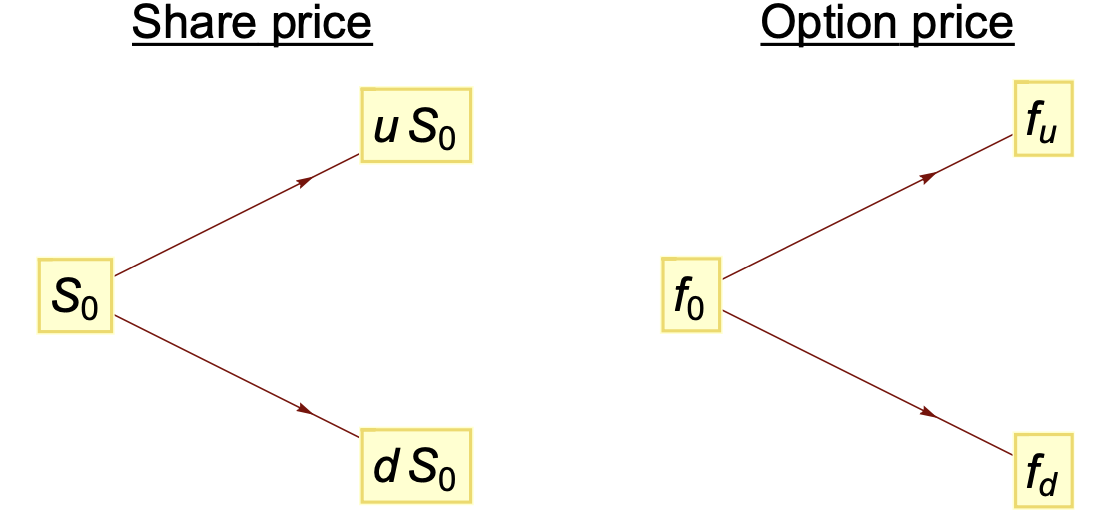
\includegraphics[scale=0.8]{Chapter4/Chapter4_1.png}
			\caption{Sum function}
		\end{figure}
	\end{example}
	
	\begin{example}
		Now let $R(Q)$ denote the revenue obtained by selling $Q$ units. Then, the profit $\pi(Q)$ is given by $\pi(Q) = R(Q) - C(Q)$.
		\\
		In the case of the firm getting a fixed price $p$ per unit, so that the graph of $R(Q)$ is a straight line through the origin. The graph of $C(Q)$ must be subtracted from that of $R(Q)$. The production level that maximises profit is $Q^*$.
		\\
		Similar to the sum function, subtracting the two graphs gives the difference graph as shown in Figure 4.4.
		\begin{figure}[ht]
			\centering
			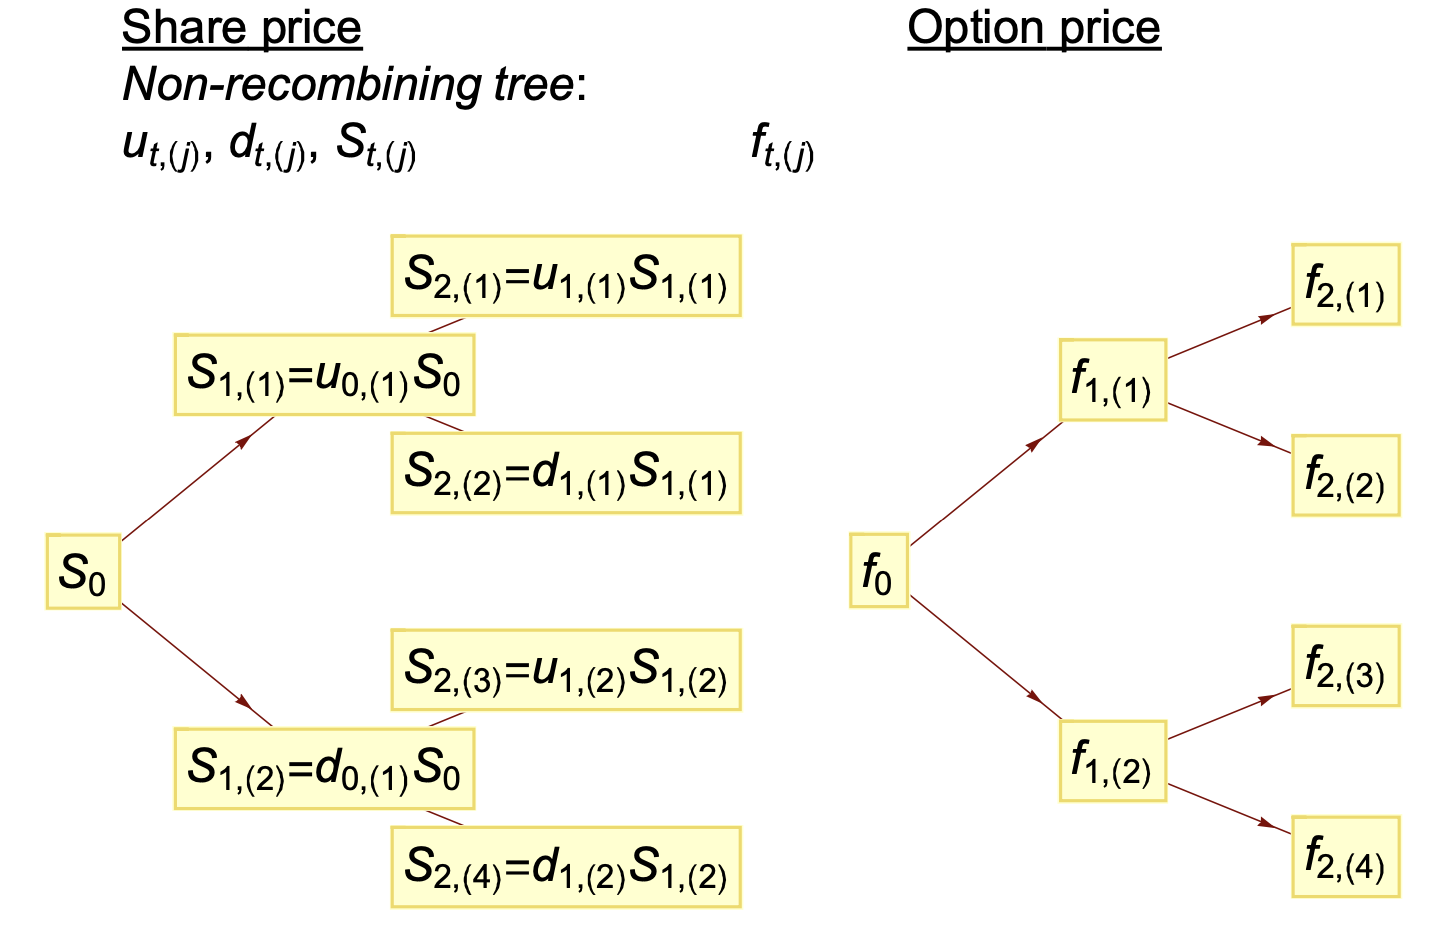
\includegraphics[scale=0.6]{Chapter4/Chapter4_2.png}
			\caption{Difference function}
		\end{figure}
	\end{example}
	
	\subsection{Products and quotients}
	If $f$ and $g$ are defined in a set $A$, the function $F$ defined by $F(x) = f(x) \cdot g(x)$ is called the \textbf{product} of $f$ and $g$, and we put $F=f \cdot g$ (or $fg$).
	\\
	The function $F$ defined where $g(x) \neq 0$ by $F(x) = f(x)/g(x) $ is called the \textbf{quotient} of $f$ and $g$, and we write $F = f/g$.
	
	\subsection{Composite functions}
	Suppose the demand for a commodity is a function $x$ of its price $p$. Suppose that price $p$ is not constant, but depends on time $t$. Then it is natural to regard $x$ as a function of $t$.
	\\
	In general, if $y$ is a function of $u$, and $u$ is a function of $x$, then $y$ can be regarded as a function of $x$. We call $y$ a \textbf{composite function} of $x$. If we denote the two functions involved by $f$ and $g$, with $y=f(u)$ and $u=g(x)$, then we can replace $u$ by $g(x)$ and so write $y$ in the form:
	$$y = f(g(x))$$
	\\
	When computing $y$, we first apply $g$ to $x$ to obtain $g(x)$, and then we apply $f$ to $g(x)$. Here $g(x)$ is called the \textbf{kernel}, or \textbf{interior function}, while $f$ is called the \textbf{exterior function}.
	\\
	The function that maps $x$ to $f(g(x))$ is often denoted by $f \circ g$. This is read as “f of g” or “f after g”, and is called the \textbf{composition} of $f$ with $g$. Correspondingly, $g \circ f$ denotes the function that maps $x$ to $g(f(x))$. Thus, we have:
	$$(f \circ g)(x) = f(g(x)) \,\,\,\,and\,\,\,\, (g \circ f)(x) = g(f(x))$$
	\\
	Note that $f \circ g$ and $g \circ f$ are usually quite different functions. For instance, if $g(x) = 2 - x^2$ and $f(u)=u^3$, then $(f \circ g)(x)=(2-x^2)^3$, whereas $(g \circ f)(x)=2-(x^3)^2 =2-x^6$; the two resulting polynomials are not the same.
	
	\begin{example}
		Write the followings as composite functions:
		\begin{enumerate}[label=(\alph*)]
			\item $y=(x^3+x^2)^{50}$
			\item $y=e^{-(x-\mu)^2}$
		\end{enumerate}
		\textbf{Solution}:
		\begin{enumerate}[label=(\alph*)]
			\item Given a value of $x$, first compute $x^3 + x^2$, which gives the interior function, $g(x) = x^3 + x^2$. Then take the 50th power of the result, so the exterior function is $f(u) = u^{50}$. Hence,
			$$f(g(x)) = f(x^3 + x^2) = (x^3 + x^2)^{50}$$
			\item We can choose the interior function as $g(x) = -(x - \mu)^2$ and the exterior function as $f(u) = e^{u}$. Alternatively, we could choose $g(x)=(x-\mu)^2$ and $f(u)=e^{-u}$.
		\end{enumerate}
	\end{example}
	
	\subsection{Symmetry}
	The function $f(x) = x^2$ satisfies $f(-x) = f(x)$, as indeed does any even power $x^2n$ , with $n$ an integer, positive or negative. So if $f (-x) = f (x)$ for all $x$ in the domain of $f$ , then $f$ is called an \textbf{even function}. This condition implies that the graph of $f$ is \textbf{symmetric} about the y-axis as shown in Fig. 4.5.
	\begin{figure}[ht]
		\centering
		\begin{tikzpicture}
			\begin{axis}[no marks, axis lines=middle,xticklabels={},yticklabels={}, xlabel=$x$, ylabel=$y$, height=0.5\textwidth]
				\addplot[samples=50] {cos(deg(x))};
			\end{axis}
		\end{tikzpicture}
		\caption{Even function}
	\end{figure}
	\\
	On the other hand, any odd power $x^{2n+1}$ such as $f (x) = ^3$ satisfies $f (-x) = -f (x)$. So if $f (-x) = -f (x)$ for all $x$ in the domain of $f$, implying that the graph of $f$ is symmetric about the origin, as shown in Fig. 4.6, then $f$ is called an \textbf{odd function}.
	\begin{figure}[ht]
		\centering
		\begin{tikzpicture}
			\begin{axis}[no marks, axis lines=middle,xticklabels={},yticklabels={}, xlabel=$x$, ylabel=$y$, height=0.5\textwidth]
				\addplot[samples=50] {sin(deg(x))};
			\end{axis}
		\end{tikzpicture}
		\caption{Odd function}
	\end{figure}
	\\
	Finally, $f$ is symmetric about $a$ if $f(a+x)=f(a-x)$ for all $x$.The graph of $f$ is then symmetric about the line $x = a$. For example, the quadratic function $f (x) = a x^2 + bx + c$ is symmetric about $x = -b/2a$. The function $y = e^{-(x-\mu})^2$ is symmetric about $x = \mu$.
	
	\begin{ex}
		Assuming $x > 0$, show graphically how to find the graph of $y = \frac{1}{4} x^2 + \frac{1}{x}$, by adding the graph of 1/x to the graph of $y = \frac{1}{4} x^2$ .
	\end{ex}
	
	\begin{ex}
		Sketch the graphs of the following functions:
		\begin{enumerate}[label=(\alph*)]
			\item $y=\sqrt{x}-x$
			\item $y=e^{x}+e^{-x}$
			\item $y=e^{-x^2}+x$
		\end{enumerate}
	\end{ex}
	
	\begin{ex}
		If $f(x)=3x-x^3$ and $g(x)=x^3$, compute:$(f+g)(x)$, $(f - g)(x)$, $(fg)(x)$, $(f/g)(x)$, $f(g(1))$, and $g(f(1))$.
	\end{ex}
	
	\begin{ex}
		Let $f(x) = 3x + 7$. Compute $f(f(x))$, and find the value $x^*$ when $f(f(x^*)) = 100$.
	\end{ex}
	
	\section{Inverse functions}
	Suppose that the demand quantity $D$ for a commodity depends on the price per unit $P$ according to $D = 30/P^{1/3}$. This formula means that the demand $D$ is corresponding to a given price $P$. 
	\\
	If we look at the matter from a producer’s point of view, however, it may be more natural to treat the output as something it can choose and consider the resulting price. This functional relationship is obtained by solving $D = 30/P^{1/3}$ for $P$.
	\\
	The two variables $D$ and $P$ in this example are related in a way that allows each to be regarded as a function of the other. In fact, the two functions:
	$$f (P) = 30p^{-1/3} \,\,\,\,and\,\,\,\, g(D) = 27000D^{-3}$$
	are \textbf{inverses} of each other.
	\\
	In general, Let $f$ be a function with domain $A$ and range $B$. If and only if $f$ is one-to-one, it has an inverse function $g$ with domain $B$ and range $A$. The function $g$ is given by the following rule: For each $y$ in $B$, the value $g(y)$ is the unique number $x$ in $A$ such that $f (x) = y$. Then
	$$g(y)=x\Leftrightarrow y=f(x)(x\in A, y\in B)$$
	
	\begin{example}
		Solve the following equations for x and find the corresponding inverse functions:
		\begin{enumerate}[label=(\alph*)]
			\item $y=4x-3$
			\item $y=\sqrt[5]{x+1}$
			\item $y=\frac{3x-1}{x+4}$
		\end{enumerate}
		\textbf{Solution}:
		\begin{enumerate}[label=(\alph*)]
			\item Solving the equation for $x$, we have the following equivalences: 
			$$y = 4 x - 3 \Leftrightarrow 4 x = y + 3 \Leftrightarrow x = \frac{1}{4} y + \frac{3}{4}$$
			for all $x$ and $y$. We conclude that $y = 4 x - 3$ and $g(y)=\frac{1}{4} y + \frac{3}{4}$ are inverses of each other.
			\item We begin by raising each side to the fifth power and so obtain the equivalences 
			$$y=\sqrt[5]{x+1} \Leftrightarrow y^5 =x+1 \Leftrightarrow x=y^5 -1$$
			These are valid for all $x$ and all $y$. Hence, we have shown that $f(x) = \sqrt[5]{x+1}$ and $g(y) = y^5 - 1$ are inverses of each other.
			\item Here we begin by multiplying both sides of the equation by the denominator and rearranging. Then we will obtain
			$$x = \frac{4y+1}{3-y}$$
			We conclude that $f(x) = (3x - 1)/(x + 4)$ and $g(y) = (4y + 1)/(3 - y)$ are inverses of each other. Observe that $f$ is only defined for $x \neq -4$, and $g$ is only defined for $y \neq 3$.
		\end{enumerate}
	\end{example}
	
	Graphically, suppose two functions $f$ and $g$ are inverses of each other. Provided that the scales of the coordinate axes are the same, the graphs of $y = f (x)$ and $y = g(x)$ are symmetric about the line $y = x$.
	
	\begin{example}
		Consider the functions $f(x)=4x-3$ and $g(x)=\frac{1}{4}x+\frac{3}{4}$ that are inverses of each other.
		\begin{figure}[ht]
			\centering
			\begin{tikzpicture}
				\begin{axis}[
					axis lines = middle,
					xmin=-4, xmax=6,
					ymin=-4, ymax=8
					]
					%first plot
					\addplot [black]{x/4+3/4};
					\node at (axis cs:5,2.5) {$y=\frac{1}{4}x+\frac{3}{4}$};
					%second plot
					\addplot [black]{4*x-3};
					\node at (axis cs:2,7) {$y=4x-3$};
					%third plot
					\addplot [black,dotted]{x};
					\node at (axis cs:4.5,5.5) {$y=x$};
				\end{axis}
			\end{tikzpicture}
			\caption{Geometric characterisation of inverse functions}
		\end{figure}
	\end{example}
	
	\begin{ex}
		Demand $D$ as a function of price P is given by $D=\frac{32}{5}- \frac{3}{10}P$. Solve the equation for $P$ and find the inverse function.
	\end{ex}
	
	\begin{ex}
		Find the domains, ranges, and inverses of the functions given by the following formulas: 
		\begin{enumerate}[label=(\alph*)]
			\item $y=-3x$
			\item $y=1/x$
			\item $y=x^3$
			\item $y=\sqrt{\sqrt{x}-2}$
		\end{enumerate}
	\end{ex}
	
	\begin{ex}
		Why does $f (x) = x^2$ , for $x$ in $(-\infty, \infty)$, have no inverse function? Show that $f$ restricted to $[0, \infty)$ has an inverse, and find that inverse.
	\end{ex}
	
	\begin{ex}
		Find inverses of the following functions, where x is the independent variable:
		\begin{enumerate}[label=(\alph*)]
			\item $f(x)=(x^3 -1)^{1/3}$
			\item $y=\frac{x+1}{x-2}$
			\item $f(x)=(1-x^3)^{1/5} +2$
		\end{enumerate}
	\end{ex}
	
	\begin{ex}
		The functions defined by the following formulas are strictly increasing in their domains. Find the domain of each inverse function, and a formula for the corresponding inverse.
		\begin{enumerate}[label=(\alph*)]
			\item $y=e^{x+4}$
			\item $y=\ln\,x-4$, $x>0$
			\item $y=\ln(2+e^{x-3}$
		\end{enumerate}
	\end{ex}
	
	\begin{ex}
		Find the inverse of $f (x) = \frac{1}{2} (e^{x} - e^{-x} )$. (Hint: Solve a quadratic equation in $z = e^{x}$.)
	\end{ex}
	
	\section{Graphs of equations}
	The equations $x\sqrt{y} = 2,\,x^2 + y^2 = 16,\,and\,y^3 + 3x^2y = 13$ are three examples of equations in two variables $x$ and $y$. A solution of such an equation is an ordered pair (a, b) such that the equation is satisfied when we replace $x$ by $a$ and $y$ by $b$. The solution set of the equation is the set of all solutions. Representing all pairs in the solution set in a Cartesian coordinate system gives a set called the graph of the equation.
	
	\begin{example}
		Find some solutions of the first two of the equations, and try to sketch their graphs.
		\\
		From $x\sqrt{y} = 2$ we obtain $y = 4/x^2$. Hence it is easy to find corresponding values for $x$ and $y$ as given in Table 4.1:
		\begin{table}[H]
			\centering
			\begin{tabular}{|c|c|c|c|c|}
				x & 1 & 2 & 4   & 6   \\
				\hline
				y & 4 & 1 & 1/4 & 1/9 
			\end{tabular}
			\caption{Solutions of $x\sqrt{y} = 2$}
		\end{table}
		
		For $x^2 + y^2 =16$, if $y=0$, $x^2=16$, so $x=\pm4$. Thus (4,0) and (-4,0) are two solutions. Table 4.2 combines these with some other solutions.
		\begin{table}[H]
			\centering
			\begin{tabular}{|c|c|c|c|c|c|c|c|}
				x & -4 & -3             & -1              & 0      & 1               & 3              & 4 \\
				\hline
				y & 0  & $\pm \sqrt{7}$ & $\pm \sqrt{15}$ & $\pm4$ & $\pm \sqrt{15}$ & $\pm \sqrt{7}$ & 0 
			\end{tabular}
			\caption{Solutions of $x^2 + y^2 =16$}
		\end{table}
	\end{example}
	
	\begin{tikzpicture}
		\begin{groupplot}[group style={group size= 2 by 1}, width=0.6\textwidth,axis lines = middle,yticklabels={}]
			\nextgroupplot[]
			\addplot[black, domain=0:6, samples = 100] {4/(x^2)};
			\node at (axis cs:2,30) {$x\sqrt{y} = 2$};
			\coordinate (top) at (rel axis cs:0,1);% coordinate at top of the first plot
			\nextgroupplot[]
			\addplot[black, domain=-4:4, samples=100] {sqrt(16-x^2)};
			\addplot[black, domain=-4:4, samples=100] {-sqrt(16-x^2)};
			\node at (axis cs:0,2) {$x^2 + y^2 =16$};
			\coordinate (bot) at (rel axis cs:1,0);% coordinate at bottom of the last plot
		\end{groupplot}
	\end{tikzpicture}
	
	\subsection{Vertical line test}
	By definition, a function assigns to each point $x$ in the domain only one $y$-value. The graph of a function, therefore, has the property that a vertical line through any point on the $x$-axis has at most one point of intersection with the graph.
	
	\begin{tikzpicture}
		\begin{groupplot}[group style={group size= 2 by 1}, width=0.6\textwidth,axis lines = middle]
			\nextgroupplot[title style={at={(0.5,0)},anchor=north,yshift=-10},
			title = A function ]
			\addplot[black, domain=0:6] {sin(deg(x)-3)};
			\addplot +[mark=none,red] coordinates {(2, -1) (2, 3)};
			\node at (axis cs:2,30) {$x\sqrt{y} = 2$};
			\coordinate (top) at (rel axis cs:0,1);% coordinate at top of the first plot
			\nextgroupplot[title style={at={(0.5,0)},anchor=north,yshift=-10},
			title = Not a function]
			\addplot[black, domain=0:4, samples=100] {sqrt(x)};
			\addplot[black, domain=0:4, samples=100] {-sqrt(x)};
			\addplot +[mark=none,red] coordinates {(2, -2) (2, 3)};
			\node at (axis cs:2,2) {$x^2 + y^2 =16$};
			\coordinate (bot) at (rel axis cs:1,0);% coordinate at bottom of the last plot
		\end{groupplot}
	\end{tikzpicture}
	\pagebreak
	
	\subsection{Compound functions}
	A function may be defined in several pieces, by giving a separate formula for each of a number of disjoint parts of the domain. Two examples of such compound functions are presented.
	
	\begin{example}
		Draw the graph of the function f defined by
		$$
		f(x)=
		\begin{cases}
			-x \,\, for \,\, x \leq 0      \\
			x^2 \,\, for \,\, 0 < x \leq 1 \\
			1.5 \,\, for \,\, x>1          
		\end{cases}
		$$
		\begin{figure}[ht]
			\centering
			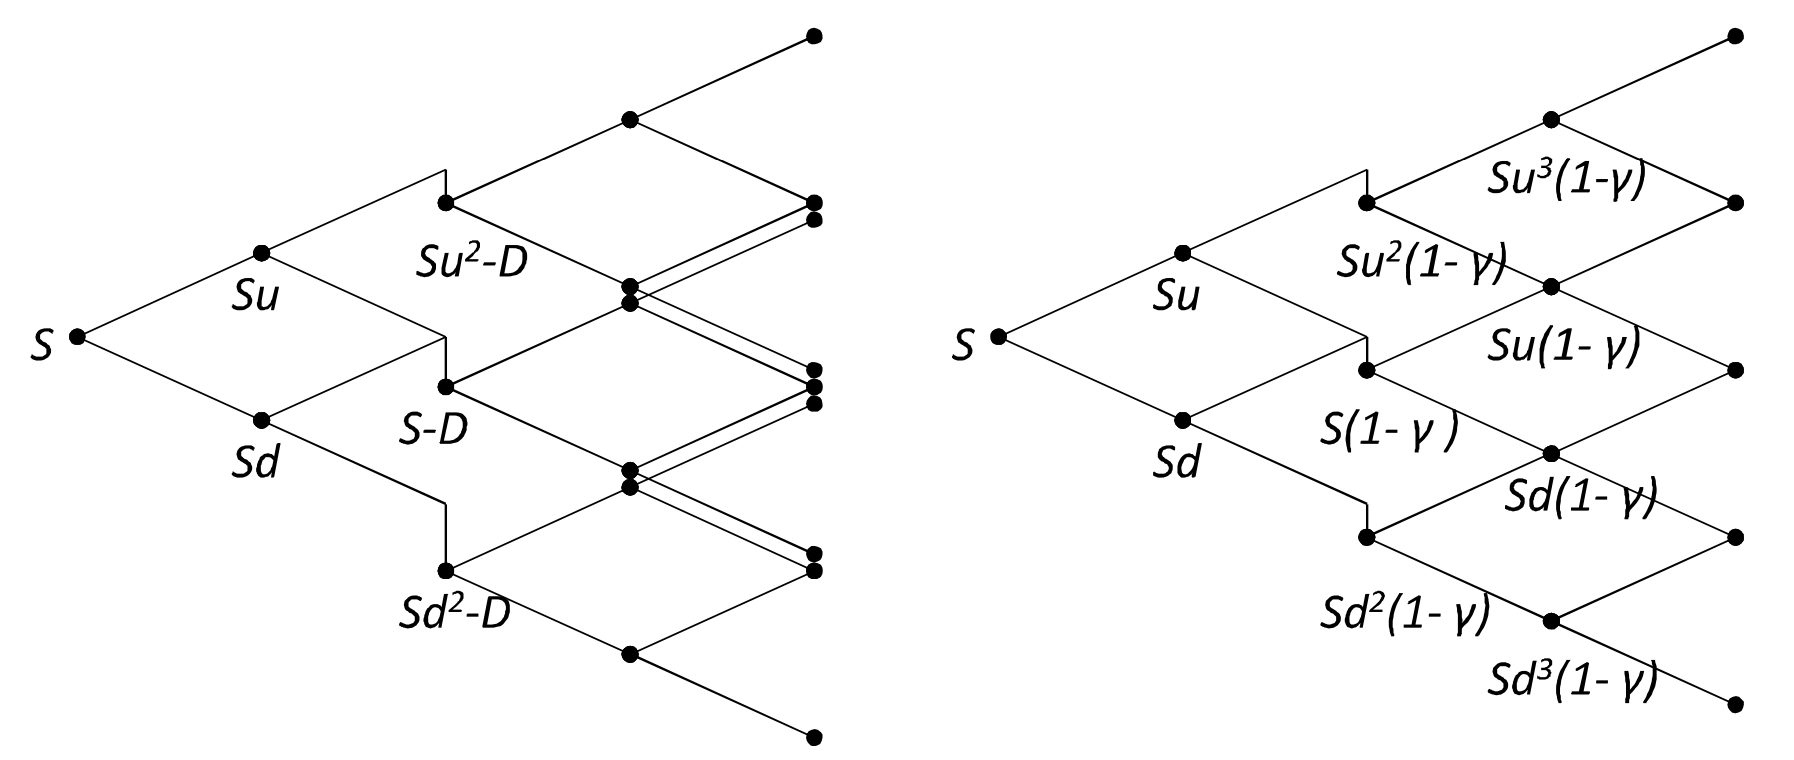
\includegraphics[scale=0.7]{Chapter4/Chapter4_3.png}
			\caption{Example of compound function}
		\end{figure}
	\end{example}
	
	\begin{ex}
		Find some particular solutions of the following two equations, then sketch their graphs:
		\begin{align*}
			& (a) \ x^2+2y^2=6 & (b) \,\,\,y^2-x^2=1 
		\end{align*}
	\end{ex}
	
	\begin{ex}
		The function $F$ is defined for all $r \geq 0$ by the following formulas:
		$$
		F(r)=
		\begin{cases}
			0 \,\,\,\,\,\,\,\,\,\,\,\,\,\,\,\,\,\,\,\,\,\,\,\,\,\,\,\,\,\,\,\,\,\,\,\,\,\,\,\,\,\,\,\,\,\,\,\,\,\,\,\,\,\,\, for \,\, r \leq7500 \\
			0.044(r-7500) \,\,\,\,\,\,\,\,\,\,\,\,\,\,\,\, for \,\, r>7500                                                                       
		\end{cases}
		$$
		Compute $F(100000)$, and sketch the graph of $F$.
	\end{ex}
	\pagebreak
	
	\section{Distance in the plane}
	Let $P_1 = (x_1, y_1)$ and $P_2 = (x_2, y_2)$ be two points in the $xy$-plane. Then by Pythagoras’s theorem, the distance $d$ between $P_1$ and $P_2$ satisfies the equation $d^2 = (x_2 - x_1)^2 + (y_2 - y_1)^2$.
	\\
	In other words, the distance between the points $(x_1, y_1)$ and $(x_2, y_2)$ is
	$$ d = \sqrt{(x_2 - x_1)^2 + (y_2 - y_1)^2} $$
	
	\begin{example}
		Find the distance $d$ between $P_1 = (-4,3)$ and $P_2 = (5,-1)$.
		\textbf{Solution}:
		$$d=\sqrt{(5-(-4))^2 + (-1-3)^2}=\sqrt{9^2+(-4)^2}=\sqrt{97}$$
	\end{example}
	
	\subsection{Circles}
	The equation of a circle with centre at $(a, b)$ and radius $r$ is $(x-a)^2 +(y-b)^2 = r^2$.
	
	\begin{example}
		Find the equation of the circle with centre at $(-4, 1)$ and radius 3.
		\textbf{Solution}: the equation of the circle is:
		$$ (x+4)^2 +(y-1)^2 = 9 $$
		\begin{figure}[ht]
			\centering
			\includegraphics[scale=0.7]{Chapter4/Chapter4_4.png}
			\caption{Circle with centre at $(-4, 1)$ and radius 3}
		\end{figure}
	\end{example}
	
	\subsection{Ellipses and hyperbolas}
	The simplest type of \textbf{ellipse} has the equation:
	$$\frac{(x-x_0)^2}{a^2}+\frac{(y-y_0)^2}{b^2}=1$$
	
	\begin{figure}[H]
		\centering
		\includegraphics[scale=0.8]{Chapter4/Chapter4_5.png}
		\caption{Example of Ellipse}
	\end{figure}
	
	Figure 4.11 shows the graphs of two \textbf{hyperbolas}:
	\begin{align*}
		& (a) \ \frac{(x-x_0)^2}{a^2}-\frac{(y-y_0)^2}{b^2}=1 & (b) \,\,\,\frac{(x-x_0)^2}{a^2}-\frac{(y-y_0)^2}{b^2}=-1 
	\end{align*}
	
	\begin{figure}[H]
		\centering
		\begin{subfigure}{0.5\textwidth}
			\centering
			\includegraphics[width=\linewidth]{Chapter4/Chapter4_6.png}
		\end{subfigure}%
		\begin{subfigure}{0.5\textwidth}
			\centering
			\includegraphics[width=\linewidth]{Chapter4/Chapter4_7.png}
		\end{subfigure}
		\caption{Examples of Hyperbola}
	\end{figure}
	
	These have \textbf{asymptotes} which are like tangents at infinity, represented by the same two dashed lines in both figures. Their equations are $y - y_0 = \pm(b/a)(x - x_0)$.
	
	Finally, consider the graph of the general quadratic equation
	$$Ax^2+Bxy+Cy^2+Dx+Ey+F=0$$
	where $A$, $B$, and $C$ are not all 0. This will have one of the following shapes:
	\begin{enumerate}[label=(\roman*)]
		\item If $4AC > B^2$, either an ellipse (possibly a circle), or a single point, or empty.
		\item If $4AC = B^2$, either a parabola, or one line or two parallel lines, or empty.
		\item If $4AC < B^2$, either a hyperbola, or two intersecting lines.
	\end{enumerate}
	
	\begin{ex}
		Determine the distances between the following pairs of points:
		\begin{align*}
			& (a) (1,3) \,\,and\,\, (2,4)     
			& (b) (-1,2) \,\,and\,\, (-3,3)   \\
			& (c) (3/2,-2) \,\,and\,\, (-5,1) 
			& (d) (x,y) \,\,and\,\, (2x,y+3)  \\
			& (e) (a,b) \,\,and\,\, (-a,b)    
			& (f) (a,3) \,\,and\,\, (2+a,5)   \\
		\end{align*}
	\end{ex}
	
	\begin{ex}
		The distance between (2, 4) and (5, $y$) is $\sqrt{13}$. Find $y$, and explain geometrically why there must be two values of $y$.
	\end{ex}
	
	\begin{ex}
		Find the equations of: 
		\begin{enumerate}[label=(\alph*)]
			\item The circle with centre at (2, 3) and radius 4.
			\item The circle with centre at (2, 5) and one point at (-1, 3).
		\end{enumerate}
	\end{ex}
	
	\begin{ex}
		Find the centre and the radius of the two circles with equations:
		\begin{enumerate}[label=(\alph*)]
			\item $x^2+y^2+10x-6y+30=0$
			\item $3x^2+3y^2+18x-24y=-39$
		\end{enumerate}
	\end{ex}
	
	\section{General functions}
	So far we have studied functions of one variable. Yet a realistic description of many economic phenomena requires considering a large number of variables simultaneously.
	\\
	An extensive discussion of functions of several variables begins in Chapter 9. This section introduces an even more general type of function.
	\\
	The general definition of a \textbf{function} is a rule which to each element in a set $A$ associates one, and only one, element in a set $B$.
	
	\begin{figure}
		\centering
		\includegraphics[scale=0.7]{Chapter4/Chapter4_8.png}
		\caption{A function from A to B}
	\end{figure}
	
	The particular value $f (x)$ is often called the \textbf{image} of the element $x$ by the function $f$. If each element of $B$ is the image of at most one element in $A$, the function $f$ is called \textbf{one-to-one}. Otherwise, if one or more elements of $B$ are the images of more than one element in $A$, the function $f$ is \textbf{many-to-one}.
	
	\begin{ex}
		Which of the following rules define functions?
		\begin{enumerate}[label=(\alph*)]
			\item The rule that assigns to each person in a classroom his or her height.
			\item The rule that assigns to each mother her youngest child alive today.
			\item The rule that assigns the perimeter of a rectangle to its area.
			\item The rule that assigns the surface area of a spherical ball to its volume.
			\item The rule that assigns the pair of numbers (x + 3, y) to the pair of numbers (x, y).
		\end{enumerate}
	\end{ex}
	
	\section{Review Exercises}
	\begin{ex}
		Use the graph of $y=|x|$ and the rules for shifting graphs to sketch the graphs of the following functions:
		\begin{enumerate}[label=(\alph*)]
			\item $y=|x|+1$
			\item $y=|x+3|$
			\item $y=3-|x+1|$
		\end{enumerate}
	\end{ex}
	
	\begin{ex}
		If $f (x) = x^3 - 2$ and $g(x) = (1 - x)x^2$, compute the six functions:
		$(f + g)(x)$; $\,\,(f - g)(x)$; $\,\,(fg)(x)$; $\,\,(f/g)(x)$; $\,\,f(g(1))$; and $\,\,g(f(1))$.
	\end{ex}
	
	\begin{ex}
		Consider the demand and supply curves $D=150- 12P$ and $S=20+2P$.
		\begin{enumerate}[label=(\alph*)]
			\item Find the equilibrium price $P^*$, and the corresponding quantity $Q^*$.
			\item Suppose a tax of \$2 per unit is imposed on the producer’s output. How will this influence the equilibrium price?
			\item Compute the total revenue obtained by the producer before the tax is imposed$(R^*)$ and after$(\hat{R})$.
		\end{enumerate}
	\end{ex}
	
	\begin{ex}
		The following functions are strictly increasing in their domains. Find the domains of their inverses and formulas for the inverses, using $x$ as the free variable.
		\begin{enumerate}[label=(\alph*)]
			\item $f(x)=3+\ln(e^x -2)$, for $x>\ln2$
			\item $f(x) = \frac{a}{e^{-\lambda x}+a}$, where $a$ and $\lambda$ are positive, for $x \in (-\infty, \infty)$
		\end{enumerate}
	\end{ex}
	
	\begin{ex}
		Determine the distances between the following pairs of points:
		\begin{align*}
			& (a) (-4,4) \,\,and\,\, (3,8)     
			& (b) (2a,3b) \,\,and\,\, (2-a,3b) 
		\end{align*}
	\end{ex}
	
	\begin{ex}
		Find the equations of the circles with:
		\begin{enumerate}[label=(\alph*)]
			\item centre at (2,-3) and radius 5
			\item centre at (-2,2) and passing through(-10,1)
		\end{enumerate}
	\end{ex}
	
	\begin{ex}
		A point $P$ moves in the plane so that it is always equidistant between the two points A = (3, 2) and B = (5, -4). Find a simple equation that the coordinates ($x$, $y$) of $P$ must satisfy. (Hint: Compute the square of the distance from $P$ to the points $A$ and $B$, respectively.)
	\end{ex}
	
	
	%============ CHAPTER 6 ===========%
	\chapter{Differentiation}
	
	\section{Slopes of curves}
	
	When we study the graph of a function, we would like to have a precise measure of its steepness at a point. We know for linear functions in the form of $y=px+q$, its slope is denoted by $p$.
	\\
	However, for an arbitrary function, we define the \textbf{slope} of a curve \textit{at a particular point} as the slope of the tangent to the point.
	\\
	As shown in the graph below, the same curve will have different slopes at different points. Suppose point $P$ has coordinates $(a,f(a)$. The slope of the curve at point $P$ is called the \textbf{derivative} of $f(x)$ at $x=a$, denoted by $f'(a)$.
	
	\begin{figure}
		\centering
		\includegraphics[scale=0.7]{Chapter5/Chapter5_1.png}
		\caption{Example of slopes at different points}
	\end{figure}
	
	\section{Tangents and derivatives}
	
	Consider a point $P$ on a curve in the $xy$-plane. Take another point $Q$ on the curve. The entire straight line through $P$ and $Q$ is called a \textbf{secant}. If we keep $P$ fixed, but let $Q$ move along the curve toward $P$, then the secant will rotate around $P$. The limiting straight line $PT$ toward which the secant tends is called the \textbf{tangent} to the curve at $P$. 
	
	\begin{figure}
		\centering
		\includegraphics[scale=0.7]{Chapter5/Chapter5_2.png}
		\caption{Secants and the tangent}
	\end{figure}
	
	Now suppose the $x$-coordinate of point $Q$ is $a+h$, where $h$ is a small number different from zero. The slope of the secant $PQ$ is therefore:
	$$\frac{f(a+h)-f(a)}{h}$$
	
	This fraction is called a \textbf{Newton quotient} of $f$. When $h$ tends to zero, the secant $PQ$ tends to the tangent. This suggests that we can define the slope of the tangent at $P$ as the number that the slope of the secant approaches as $h$ tends to 0. Formally:
	
	The derivative of function $f$ at point $a$, denoted by $f'(a)$, is 
	$$f'(a) = \lim_{h \rightarrow 0} \frac{f(a+h)-f(a)}{h}$$
	
	The equation for the tangent to the graph of $y = f (x)$ at the point $(a, f (a))$ is
	$$y - f (a) = f '(a)(x - a)$$
	
	
	\begin{example}
		Use the definition of slope to compute $f'(x)$ when $f(x)=x^2$. Find in particular $f '(1/2)$ and $f '(-1)$. Give geometric interpretations, and find the equation for the tangent at each of the points $(1/2, 1/4)$ and $(-1, 1)$.
		\\
		\textbf{Solution}:
		\\
		For $f(x)=x^2$, we have $f(x+h)=(x+h)^2 =x^2 +2xh+h^2$, so
		$$f(x+h) - f(x) = (x^2+2xh+h^2)-x^2 = 2xh + h^2$$
		For all $h \neq 0$, the Newton quotient is:
		$$\frac{f(x+h)-f(x)}{h} = \frac{2xh+h^2}{h} = 2x + h$$
		Therefore we can obtain
		$$f'(x) = \lim_{h \rightarrow 0} \frac{f(x+h)-f(x)}{h} = \lim_{h \rightarrow 0} (2x+h) = 2x$$
		When $x = 1/2$, we obtain $f '(1/2) = 2 \times 1/2 = 1$. Similarly, $f '(-1) = 2 \times (-1) = -2$.
		
		\begin{figure}
			\centering
			\includegraphics[scale=0.7]{Chapter5/Chapter5_3.png}
			\caption{Geometric interpretation}
		\end{figure}
		
		At $(1/2,1/4)$, the equation of the tangent is $y-1/4 = 1 \times (x-1/2)$ or $y = x - 1/4$. Similarly, the equation of the tangent at point $(-1,1)$ is $y=-2x-1$.
	\end{example}
	
	A commonly used form of notation for derivatives is the \textbf{differential notation} due to Leibniz. If $y=f(x)$, then in place of $f'(x)$, we write $\frac{dy}{dx}$, $\frac{df(x)}{dx}$ or $\frac{d}{dx}f(x)$.
	\\
	We can think of the symbol "d/dx" as an instruction to differentiate what follows with respect to $x$. Differentiation occurs so often in mathematics that it has become standard to use w.r.t. as an abbreviation for with respect to.
	
	When we use letters other than $f$ , $x$, and $y$, the notation for the derivative changes accordingly. For example:
	$P(t)=t^2 \Rightarrow P'(t)=2t$; $Y =K^3 \Rightarrow Y' =3K^2$; and $A=r^2 \Rightarrow dA =2r$.
	
	\begin{ex}
		Let $f(x)=3x^2 +2x-1$.
		\begin{enumerate}[label=(\alph*)]
			\item Show that $f(x+h)-f(x) =6x+2+3h$ for $h \neq 0$, and use this result to find $f'(x)$.
			\item Find in particular $f'(0)$, $f'(-2)$, and $f'(3)$. Find also the equation of the tangent to the graph at the point $(0, -1)$.
		\end{enumerate}
	\end{ex}
	
	\begin{ex}
		The demand function for a commodity with price $P$ is given by the formula $D(P) = a - bP$ and the cost of producing $x$ units of a commodity is given by the formula $C(x) = p + qx^2$. Use the rule of differentiation to find $dD(P)/dP$ and $C'(x)$.
	\end{ex}
	
	\begin{ex}
		Show that $[f(x + h) - f(x)]/h = -1/x(x + h)$, and use this to show that
		$$f(x)= \frac{1}{x} =x^{-1} \Rightarrow f'(x)=\frac{-1}{x^2} = -x^{-2}$$
	\end{ex}
	
	\begin{ex}
		In each case below, find the slope of the tangent to the graph of $f$ at the specified point:
		\begin{align*}
			& (a) f(x)=3x+2 \,\, at \,\,(0,2)    
			& (b) f(x)=x^2-1 \,\, at \,\,(1,0)   \\
			& (c) f(x)=2+3/x \,\, at \,\,(3,3)   
			& (d) f(x)=x^3-2x \,\, at \,\,(0,0)  \\
			& (e) f(x)=x+1/x \,\, at \,\,(-1,-2) 
			& (f) f(x)=x^4 \,\, at \,\,(1,1)     \\
		\end{align*}
	\end{ex}
	
	\begin{ex}
		Figure 5.4 shows the graph of a function $f$. Determine the sign of the derivative $f'(x)$ at each of the four points $a$, $b$, $c$, and $d$.
		\begin{figure}[ht]
			\centering
			\includegraphics[scale=0.7]{Chapter5/Chapter5_4.png}
			\caption{Exercise 5.5}
		\end{figure}
	\end{ex}
	
	\begin{ex}
		Let $f(x)=\sqrt{x}$.
		\begin{enumerate}[label=(\alph*)]
			\item Show that $(\sqrt{x+h}-\sqrt{x})(\sqrt{x+h}+\sqrt{x})=h$
			\item Use the result in part (a) to show that the Newton quotient of $f(x)$ is $1/(\sqrt{x+h}+\sqrt{x})$.
			\item Use the result in part (b) to show that for $x>0$, $f'(x) = \frac{1}{2\sqrt{x}}=\frac{1}{2}x^{-1/2}$
		\end{enumerate}
	\end{ex}
	
	\begin{ex}
		Apply the results of Ex 5.5 to prove first that
		$$[(x+h)^{1/3} - x^{1/3}][(x+h)^{2/3} +(x+h)^{1/3}x^{1/3} +x^{2/3}]=h
		$$
		Then follow the argument used to solve Ex 5.5 to show that $f (x) = x^{1/3} \Rightarrow  f' (x) = \frac{1}{3}x^{-2/3} $.
	\end{ex}
	
	\section{Increasing and decreasing functions}
	Assume that $f$ is defined in an interval $I$ and that $x_1$ and $x_2$ are numbers from that interval.
	\begin{enumerate}[label=(\roman*)]
		\item If $f (x_2) \geq f (x_1)$ whenever $x_2 > x_1$, then $f$ is \textit{increasing} in $I$.
		\item If $f (x_2) > f (x_1)$ whenever $x_2 > x_1$, then $f$ is \textit{strictly increasing} in $I$.
		\item If $f (x_2) \leq f (x_1)$ whenever $x_2 > x_1$, then $f$ is \textit{decreasing} in $I$.
		\item If $f (x_2) < f (x_1)$ whenever $x_2 > x_1$, then $f$ is \textit{strictly decreasing} in $I$.
	\end{enumerate}
	
	We can also test whether a function is increasing or decreasing by checking the sign of its derivative:
	\begin{align*}
		f'(x) \geq 0 \text{ for all } x \text{ in the interval } I & \Leftrightarrow f \text{ is increasing in } I \\
		f'(x) \leq 0 \text{ for all } x \text{ in the interval } I & \Leftrightarrow f \text{ is decreasing in } I \\
		f'(x) = 0 \text{ for all } x \text{ in the interval } I    & \Leftrightarrow f \text{ is constant in } I   
	\end{align*}
	
	\begin{example}
		Find the derivative of $f(x)= \frac{1}{2}x^2 -2$.Then examine whether $f$ is increasing or decreasing.
		\\
		\textbf{Solution}:
		\\
		We find that $f'(x) = x$, which is non-negative for $x \geq 0$, and non-positive if $x \leq 0$, and thus $f'(0) = 0$. We conclude that $f$ is increasing in $[0, \infty)$ and decreasing in $(-\infty, 0]$.
	\end{example}
	
	\begin{ex}
		Examine whether $f (x) = x^2 - 4x + 3$ is increasing or decreasing.
	\end{ex}
	
	\begin{ex}
		Examine whether $f (x) = -x^3 + 4x^2 - x - 6$ is increasing or decreasing.
	\end{ex}
	
	\begin{ex}
		Show algebraically that $f (x) = x^3$ is strictly increasing by studying the sign of
		$$x_2^3 - x_1^3 =(x_2 - x_1)(x_1^2 +x_1x_2 +x_2)=(x_2 - x_1) \left[ \left(x_1 + 2x_2)^2 \right) + \frac{3}{4}x_2^2 \right]$$
	\end{ex}
	
	\section{Rates of change}
	The derivative can be interpreted in many ways, one of which is the \textbf{rate of change}. The Newton quotient can be interpreted as the \textit{average rate of change of f over the interval from a to a+h}.
	\\
	Taking the limit as $h$ tends to 0 gives the derivative of $f$ at $a$, which we interpret as the \textbf{instantaneous rate of change}.
	\\
	Sometimes we are interested in studying the proportion $f'(a)/f(a)$. This proportion can be interpreted as the \textbf{relative rate of change}.
	
	\begin{example}
		Consider a firm producing some commodity in a given period, and let $C(x)$ denote its cost of producing $x$ units. The derivative $C'(x)$ at $x$ is called the \textbf{marginal cost} at $x$. According to the definition, it is equal to
		$$C'(x) = \lim_{h \rightarrow 0} \frac{C(x + h) - C(x)}{h}$$
		When $h$ is small in absolute value, we obtain the approximation $$C'(x) \approx \frac{ C(x + h) - C(x)}{h}$$
		The difference $C(x + h) - C(x)$ is called the \textbf{incremental cost} of producing $h$ units of extra output. For $h$ small, a linear approximation to this incremental cost is $hC'(x)$, the product of the marginal cost and the change in output. This is true even when $h < 0$, signifying a decrease in output and, provided that $C'(x) > 0$, a lower cost.
		\\
		Note that putting $h = 1$ makes marginal cost approximately equal to
		$$C'x) \approx C(x + 1) - C(x)$$
		Marginal cost is then approximately equal to the incremental cost $C(x + 1) - C(x)$, that is, the additional cost of producing one more unit than $x$.
	\end{example}
	
	\begin{example}
		Let $C(x)$ denote the cost in millions of dollars for removing $x$\% of the pollution in a lake. Give an economic interpretation of the equality $C'(50) = 3$.
		\\
		\textbf{Solution}:
		\\
		Because of the linear approximation $C(50 + h) - C(50) \approx h C'(50)$, the precise interpretation of $C'(50) = 3$ is that, starting at 50\%, for each extra 1\% of pollution that is removed, the extra cost is about 3 million dollars. Much less precisely, $C'(50) = 3$ means that it costs about 3 million dollars extra to remove 51\% instead of 50\% of the pollution.
	\end{example}
	
	\begin{ex}
		Let $C(x) = x^2 + 3x + 100$ be the cost function of a firm. Show that when $x$ is changed from 100 to 100 + $h$, where $h \neq 0$, the average rate of change per unit of output is
		$$\frac{C(100+h)-C(100)}{h} = 203+h$$
		What is the marginal cost $C'(100)$? Use the definition of derivatives to find $C'(x)$ and in particular $C'(100)$.
	\end{ex}
	
	\begin{ex}
		If the cost function of a firm is $C(x) = \Bar{C} + cx$, give economic interpretations of the parameters $c$ and $\Bar{C}$.
	\end{ex}
	
	\begin{ex}
		If the total saving of a country is a function $S(Y)$ of the national product $Y$, then $S'(Y)$ is called the \textbf{marginal propensity to save}, or MPS. Find the MPS for the following functions:
		\begin{align*}
			& (a) S(Y)= \Bar{S} + sY      
			& (b) S(Y)=100+0.1Y+0.0002Y^2 
		\end{align*}
	\end{ex}
	
	\section{Limits}
	
	Suppose, in general, that a function $f$ is defined for all $x$ near $a$, but not necessarily at $x = a$. Then we say that the number $A$ is the limit of $f (x)$ as $x$ tends to $a$ if $f (x)$ tends to $A$ as $x$ tends to (but is not equal to) $a$. We write:
	$$\lim_{x \rightarrow a} f(x)=A, \,\,\,\,\,or \,\,f(x)\rightarrow A \,\,as\,\,x \rightarrow a$$
	
	Consider the function
	$$F(x) = \frac{e^x-1}{x}$$
	The function is not defined for $x=0$ but we can still find the values of $F(x)$ when $x$ is close to zero.
	
	\begin{table}[ht]
		\centering
		\begin{tabular}{|c|c|c|c|c|c|c|c|c|c|}
			\hline
			x      & -1    & -0.1  & -0.001 & -0.0001 & 0           & 0.0001 & 0.001 & 0.1   & 1     \\
			\hline
			$F(x)$ & 0.632 & 0.956 & 0.999  & 1.000   & Not defined & 1.000  & 1.001 & 1.052 & 1.718 \\
			\hline
		\end{tabular}
		\caption{Values of $F(x)$ when $x$ is close to 0}
	\end{table}
	
	So we can write:
	$$\lim_{x \rightarrow 0} \frac{e^x-1}{x}=1 \,\, or \,\, \frac{e^x-1}{x} \rightarrow 1 \,\, as \,\, x \rightarrow 0 $$.
	
	General rules for limits:
	
	If $\lim_{x \rightarrow a} f(x) = A$ and $\lim_{x \rightarrow a} g(x) = B$, then:
	\begin{align*}
		\lim_{x \rightarrow a} [f(x) \pm g(x)]   & = A \pm B                                                                  \\
		\lim_{x \rightarrow a} [f(x) \cdot g(x)] & = A \cdot B                                                                \\
		\lim_{x \rightarrow a} \frac{f(x)}{g(x)} & = \frac{A}{B} \text{,  if } B \neq 0                                       \\
		\lim_{x \rightarrow a} [f(x)]^r          & = A^r \text{,  if } A^r \text{ is defined and } r \text{ is a real number} 
	\end{align*}
	
	\begin{example}
		Use the rules for limits to compute the following limits:
		\begin{equation*}
			(a) \lim_{x \rightarrow -2}(x^2+5x) \quad
			(b) \lim_{x \rightarrow 4} \frac{2x^{3/2}-\sqrt{x}}{x^2-15} \qquad
			(c) \lim_{x \rightarrow a} Ax^n
		\end{equation*}
		
		\textbf{Solution}:
		\begin{enumerate}[label=(\alph*)]
			\item The limit can be expressed as:
			$$\lim_{x \rightarrow -2}x \cdot \lim_{x \rightarrow -2}x + \lim_{x \rightarrow -2}5 \cdot \lim_{x \rightarrow -2}x$$
			So
			$$\lim_{x \rightarrow -2}(x^2+5x) = (-2)(-2)+5(-2) = -6$$
			\item Similar to (a), the limit can be expressed as:
			$$\lim_{x \rightarrow 4}\frac{2x^{3/2}-\sqrt{x}}{x^2-15}=\frac{2 \lim_{x \rightarrow 4} x^{3/2} - \lim_{x \rightarrow 4}\sqrt{x}}{\lim_{x \rightarrow 4} x^2 - 15} = \frac{2 \cdot 4^{3/2}-\sqrt{4}}{4^2-15}=14$$
			\item Finally,
			$$\lim_{x \rightarrow a}Ax^n = \lim_{x \rightarrow a}A \cdot \lim_{x \rightarrow a}x^n = A \cdot (\lim_{x \rightarrow a}x)^n = A \cdot a^n$$
			where $n$ is a natural number.
		\end{enumerate}
	\end{example}
	
	\begin{ex}
		Determine the following by using the rules for limits:
		\begin{equation*}
			(a) \lim_{x \rightarrow 0}(3+2x^2) \qquad
			(b) \lim_{x \rightarrow -1} \frac{3+2x}{x-1} \qquad
			(c) \lim_{x \rightarrow 2} (2x^2+5)^3
		\end{equation*}
		\begin{equation*}
			(d) \lim_{t \rightarrow 8}(5t+t^2-\frac{1}{8}t^3) \qquad
			(e) \lim_{y \rightarrow 0} \frac{(y+1)^5-y^5}{y+1} \qquad
			(f) \lim_{z \rightarrow -2} \frac{1/z+2}{z}
		\end{equation*}
	\end{ex}
	
	\begin{ex}
		If $f(x) = x^2+2x$, compute the following limits:
		\begin{equation*}
			(a) \lim_{x \rightarrow 1}\frac{f(x)-f(1)}{x-1} \qquad
			(b) \lim_{h \rightarrow 0} \frac{f(2+h)-f(2)}{h} \qquad
			(c) \lim_{h \rightarrow 0} \frac{f(a+h)-f(a-h)}{h}
		\end{equation*}
	\end{ex}
	
	\begin{ex}
		Compute the following limits, where in part (c) $n$ denotes any natural number:
		\begin{equation*}
			(a) \lim_{x \rightarrow 2}\frac{x^2-2x}{x^3-8} \qquad
			(b) \lim_{h \rightarrow 0} \frac{\sqrt[3]{27+h}-3}{h} \qquad
			(c) \lim_{x \rightarrow 1} \frac{x^n-1}{x-1}
		\end{equation*}
	\end{ex}
	
	\section{Simple rules for differentiation}
	
	If $f$ is a constant function, then its derivative is 0:
	$$f(x) = A \Rightarrow f'(x) = 0$$
	
	When taking derivatives, additive constants disappear while multiplicative constants are preserved:
	\begin{align*}
		y = A + f(x) & \Rightarrow y' = f'(x)  \\
		y = Af(x)    & \Rightarrow y' = Af'(x) 
	\end{align*}
	
	The \textbf{power rule} is that given any constant $a$,
	$$f(x) = x^a \Rightarrow f'(x) = ax^{a-1}$$
	
	\begin{example}
		Use the power rule to compute:
		\begin{equation*}
			(a) \frac{d}{dx} (\frac{x^{100}}{100}) \qquad
			(b) \frac{d}{dx} (x^{-0.33}) \qquad
			(c) \frac{d}{dr} (-5r^{-3}) \qquad
		\end{equation*}
		\begin{equation*}
			(d) \frac{d}{dp} (Ap^{\alpha}+B) \qquad
			(e) \frac{d}{dx} (\frac{A}{\sqrt{x}})
		\end{equation*}
		\\
		\textbf{Solution}:
		\begin{enumerate}[label=(\alph*)]
			\item $\frac{d}{dx} (\frac{x^{100}}{100}) = \frac{1}{100} 100x^{100-1} = x^{99}$
			\item $\frac{d}{dx} (x^{-0.33}) = -0.33x^{-0.33-1} = -0.33x^{-1.33}$
			\item $\frac{d}{dr} (-5r^{-3}) = (-5)(-3)r^{-3-1} = 15r^{-4}$
			\item $\frac{d}{dp} (Ap^{\alpha}+B) = A\alpha p^{\alpha-1}$
			\item $\frac{d}{dx} (\frac{A}{\sqrt{x}}) = \frac{d}{dx} (Ax^{-1/2}) = A(-\frac{1}{2})x^{-1/2-1} = -\frac{1}{2}Ax^{-3/2}$
		\end{enumerate}
	\end{example}
	
	\begin{ex}
		Compute the following:
		\begin{equation*}
			(a) \frac{d}{dr}(4\pi r^2) \qquad
			(b) \frac{d}{dy} (Ay^{b+1}) \qquad
			(c) \frac{d}{dA} \left( \frac{1}{A^2 \sqrt{A}} \right)
		\end{equation*}
	\end{ex}
	
	\section{Sums, Products, and Quotients}
	
	\subsection{Sums and Differences}
	Suppose $f$ and $g$ are both defined on a set $A$ of real numbers. If both $f$ and $g$ are differentiable at $x$, then the sum $f + g$ and the difference $f - g$ are both differentiable at $x$, with
	$$F(x) = f(x) \pm g(x) \Rightarrow F'(x) = f'(x) \pm g'(x)$$
	
	\begin{example}
		Compute $\frac{d}{dx} (3x^8+x^{100}/100)$.
		\\
		\textbf{Solution}:
		
		$$\frac{d}{dx} (3x^8+x^{100}/100) = \frac{d}{dx} (3x^8) + \frac{d}{dx}(x^{100}/100) = 24x^7 + x^{99}$$
	\end{example}
	
	\subsection{Products}
	
	If both $f$ and $g$ are differentiable at the point $x$, then so is $F = f \cdot g$, and
	$$F(x) = f(x) \cdot g(x) \Rightarrow  F'(x) = f'(x) \cdot g(x) + f(x) \cdot g'(x)$$
	
	\begin{example}
		Find $h'(x)$ when $h(x)=(x^3 -x)·(5x^4 +x^2)$. Confirm the answer by expanding $h(x)$ as a single polynomial, then differentiating the result.
		
		\textbf{Solution}:
		
		We see that $h(x)=f(x) \cdot g(x)$ with $f(x)=x^3 -x$ and $g(x)=5x^4 +x^2$. Here $f'(x) = 3x^2 - 1$ and $g'(x) = 20x^3 + 2x$. Thus from the products rule:
		$$h'(x) = (3x^2-1) \cdot (5x^4+x^2) + (x^3-x) \cdot (20x^3+2x) = 35x^6 - 20x^4 - 3x^2$$
		
		Alternatively, expanding $h(x)$ as a polynomial gives $h(x) = 5x^7 - 4x^5 - x^3$, which gives the same derivative.
	\end{example}
	
	\subsection{Quotients}
	If $f$ and $g$ are differentiable at $x$ and $g(x)  \neq 0$, then $F = f /g$ is differentiable at $x$, and
	$$F(x) = \frac{f(x)}{g(x)} \Rightarrow F'(x) = \frac{f'(x) \cdot g(x) - f(x) \cdot g'(x)}{(g(x))^2}$$
	
	\begin{example}
		Compute $F'(x)$ and $F'(4)$ when
		$$F(x) = \frac{3x-5}{x-2}$$
		
		\textbf{Solution}:
		
		We apply the quotient rule with $f(x) = 3x-5$ and $g(x) = x-2$. Then $f'(x) = 3$ and $g'(x) = 1$. So we obtain, for $x \neq 2$:
		$$F'(x) = \frac{3 \cdot (x-1) - (3x-5) \cdot 1}{(x-2)^2} = \frac{-1}{(x-2)^2}$$ 
		
		To find $F'(4)$, we put $x=4$ in the formula and obtain $F'(4) = -1/4$.
	\end{example}
	
	\begin{ex}
		Differentiate w.r.t $x$ the following functions:
		\begin{equation*}
			(a) \frac{3}{5}x^2-2x^7+\frac{1}{8}-\sqrt{x} \qquad
			(b) (2x^2-1)(x^4-1) \qquad
			(c) \left( x^5+\frac{1}{x} \right) (x^5+1)
		\end{equation*}
	\end{ex}
	
	\begin{ex}
		Differentiate w.r.t $x$ the following functions:
		\begin{equation*}
			(a) \frac{\sqrt{x}-2}{\sqrt{x}+1} \qquad
			(b) \frac{x^2-1}{x^2+1} \qquad
			(c) \frac{x^2+x+1}{x^2-x+1}
		\end{equation*}
	\end{ex}
	
	\begin{ex}
		For each of the following functions, determine the intervals where it is increasing.
		\begin{equation*}
			(a) y=3x^2-12x+13 \qquad
			(b) y=\frac{1}{4}(x^4-6x^2) \qquad
			(c) y=\frac{x^2-x^3}{2(x+1)}
		\end{equation*}
	\end{ex}
	
	\begin{ex}
		Find the equations for the tangents to the graphs of the following functions at the specified points:
		\begin{align*}
			& (a) y=3-x-x^2 \,\,at\,\, x=1                                 
			& (b) y=\frac{x^2-1}{x^2+1} \,\,at\,\,x=1                      \\
			& (c) y= \left ( \frac{1}{x^2}+1 \right) (x^2-1) \,\,at\,\,x=2 
			& (d) y=\frac{x^4+1}{(x^2+1)(x+3)} \,\,at\,\,x=0               \\
		\end{align*}
	\end{ex}
	
	\section{Chain rule}
	
	The \textbf{chain rule} states that if $y$ is a differentiable function of $u$, and $u$ is a differentiable function of $x$, then $y$ is a differentiable function of $x$, and
	$$\frac{dy}{dx}= \frac{dy}{du} \cdot \frac{du}{dx}$$
	
	The generalised power rule is that if $y=u^a$ and $u$ is a differentiable function of $x$, then
	$$y' = au^{a-1}u'$$
	
	\begin{example}
		Find dy/dx when:
		\begin{enumerate}[label=(\alph*)]
			\item $y=u^5$ and $u=(1-x^3)$
			\item $y=\frac{10}{(x^2+4x+5)^7}$
		\end{enumerate}
		\textbf{Solution:}
		
		\begin{enumerate}[label=(\alph*)]
			\item Here we apply the chain rule directly. Since $dy/du = 5u^4$ and $du/dx= -3x^2$, we have
			$$\frac{dy}{dx} = \frac{dy}{du}\cdot \frac{du}{dx} = 5u^4(-3x^2) = -15x^2 u^4 = -15x^2 (1-x^3)^4$$
			\item If we write $u = x^2 + 4x + 5$, then $y = 10u^{-7}$. By the generalised power rule, one has
			$$\frac{dy}{dx} = 10(-7)u^{-8}u' = 5u^4(-3x^2) = -70u^{-8}(2x+4) = \frac{-140(x+2)}{(x^2+4x+5)^8}$$
		\end{enumerate}
	\end{example}
	
	\subsection{Alternative formulation of the chain rule}
	
	Consider a composite function $y=f(g(x))$. If $g$ is differentiable at $x_0$ and $f$ is differentiable at $u_0 = g(x_0)$, then the composite function $F(x) = f (g(x))$ is differentiable at $x_0$, and
	$$F'(x_0) = f'(u_0)g'(x_0) = f'(g(x_0))g'(x_0)$$
	
	\begin{example}
		Find the derivative of the compound function $F(x) = f (g(x))$ at $x_0 = -3$ in case $f(u)=u^3$ and $g(x) = 2-x^2$.
		
		\textbf{Solution}:
		
		In this case we have $f'(u) = 3u^2$ and $g'(x) = -2x$. So according to the alternative formulation of the chain rule, one has $F'(-3)=f'(g(-3))g'(-3)$. Now $g(-3)=2-(-3)^2 =2-9=-7$; $g'(-3)=6$; and $f'(g(-3)) = f'(-7) = 3(-7)^2 = 3 \cdot 49 = 147$. So $F'(-3) = f'(g(-3))g'(-3) = 147 \cdot 6 = 882$.
	\end{example}
	
	\begin{ex}
		Find the derivatives of the following functions:
		\begin{equation*}
			(a) y=\frac{1}{(x^2+x+1)^5} \qquad
			(b) y=\sqrt{x+\sqrt{x+\sqrt{x}}} \qquad
		\end{equation*}
	\end{ex}
	
	\begin{ex}
		Suppose that $C=20q-40q(25-\frac{1}{2}x)^{\frac{1}{2}}$, where $q$ is a constant and $x<50$. Find d$C$/d$x$.
	\end{ex}
	
	\section{Higher-order derivatives}
	The derivative $f'$ of a function $f$ is often called the first derivative of $f$. If $f'$ is also differentiable, then we can differentiate $f'$ in turn. The result $(f')'$ is called the second derivative, written more concisely as $f''$.
	\\
	Similarly, a function $f(x)$ may have third, forth derivatives and so on. In general, the n-th derivative of $f$ at x is expressed as:
	$$y^{(n)} = f^{(n)}(x) \,\, or \,\, \frac{d^ny}{dx^n}$$
	The number $n$ is the \textbf{order} of the derivative.
	
	A different form of notation is:
	$$f''(x) = \frac{d^2f(x)}{dx^2} \,\,or\,\, y''=\frac{d^2y}{dx^2} $$
	
	\begin{example}
		Find $f'(x)$ and $f''(x)$ when $f(x) = 2x^5-3x^3+2x$
		
		\textbf{Solution}:
		
		The rules for differentiating polynomials imply that $f'(x) = 10x^4 - 9x^2 + 2$. Then we differentiate each side of this equality to get $f''(x) = 40x^3 - 18x$.
	\end{example}
	
	Recall that the sign of the first derivative determines whether a function is increasing or decreasing on an interval $I$. Then the second derivative implies:
	\begin{align*}
		f''(x) \geq 0 \text{ on } I & \Leftrightarrow f' \text{ is increasing in } I \\
		f''(x) \leq 0 \text{ on } I & \Leftrightarrow f' \text{ is decreasing in } I \\
	\end{align*}
	
	Graphical visualisations are:
	\begin{figure}[H]
		\centering
		\includegraphics[scale=0.7]{Chapter5/Chapter5_5.png}
		\caption{The slope of the tangent line increases as x increases}
	\end{figure}
	
	\begin{figure}[H]
		\centering
		\includegraphics[scale=0.7]{Chapter5/Chapter5_6.png}
		\caption{The slope of the tangent line decreases as x increases}
	\end{figure}
	
	Suppose that $f$ is continuous in the interval $I$ and twice differentiable in the interior of $I$. Then we can introduce the following definitions:
	\begin{align*}
		f \text{ is \textit{convex} on } I  & \Leftrightarrow f'' \geq 0 \text{ for all $x$ in } I \\
		f \text{ is \textit{concave} on } I & \Leftrightarrow f'' \leq 0 \text{ for all $x$ in } I \\
	\end{align*}
	
	\begin{example}
		Check the convexity/concavity of the following functions:
		\begin{equation*}
			(a) f(x)=x^2-2x+2 \qquad
			(b) f(x)=ax^2+bx+c \qquad
		\end{equation*}
		
		\textbf{Solution}:
		\begin{enumerate}[label=(\alph*)]
			\item Here $f'(x) = 2x - 2$ so $f''(x) = 2$. Because $f''(x) > 0$ for all $x$, the function $f$ is convex.
			\item Here $f'(x) = 2ax + b$, so $f''(x) = 2a$. If $a = 0$, then $f$ is linear, so it is both concave and convex. If $a>0$,then $f''(x)>0$, so $f$ is convex. If $a<0$,then $f''(x)<0$, so $f$ is concave.
		\end{enumerate}
	\end{example}
	
	\begin{ex}
		Compute the second derivative of:
		\begin{enumerate}[label=(\alph*)]
			\item $y=x^5-3x^4+2$
			\item $y=\sqrt{x}$
			\item $y=(1+x^2)^{\frac{1}{2}}$
		\end{enumerate}
	\end{ex}
	
	\begin{ex}
		Find $g''(2)$ when $g(t) = \frac{t^2}{t-1}$
	\end{ex}
	
	\section{Exponential functions}
	
	Derivative of the natural exponential function:
	$$f(x) = e^x \,\, \Rightarrow \,\, f'(x) = e^x$$
	
	\begin{example}
		Find the first and second derivatives of:
		\begin{equation*}
			(a) y=x^3+e^x \qquad
			(b) y=x^5e^x \qquad
			(c) y=e^x/x
		\end{equation*}
		
		\textbf{Solution}:
		\begin{enumerate}[label=(\alph*)]
			\item We can easily find that $y'=3x+e^x$ and $y''=6x+e^x$.
			\item By the product rule, $y'=5x^4 e^x + x^5 e^x$. To find the second derivative, differentiate $y'$ once more to obtain $y''=20x^3e^x+5x^4e^x+5x^4e^x+x^5e^x = 20x^3e^x+10x^4e^x+x^5e^x$.
			\item The quotient rule yields:
			$$y'=\frac{e^xx-e^x \cdot 1}{x^2}=\frac{e^x(x-1)}{x^2}$$
			Differentiating again gives:
			$$y''=\frac{(e^xx+e^x-e^x)x^2-(e^xx-e^x)2x}{(x^2)^2}=\frac{e^x(x^2-2x+2)}{x^3}$$.
		\end{enumerate}
	\end{example}
	
	\begin{example}
		For each of the following functions, find the intervals where they are increasing:
		\begin{equation*}
			(a)y=\frac{e^x}{x} \qquad
			(b)y=x^4e^{-2x} \qquad
			(c)y=xe^{-\sqrt{x}}
		\end{equation*}
		
		\textbf{Solution}:
		\begin{enumerate}[label=(\alph*)]
			\item As shown in the previous example, $y'=e^x(x-1)/x^2$, so $y'\geq 0$ if and only if $x \geq 1$. Thus $y$ is increasing in $[1,\infty)$.
			\item We can easily obtain $y'=x^3e^{-2x}(4-2x)$. A sign diagram reveals that $y$ is increasing in [0,2].
			\item The function is only defined for $x \geq 0$. Using the chain rule and product rule, the derivative of $y$ is:
			$$y'=1\cdot e^{-\sqrt{x}}-\frac{xe^{-\sqrt{x}}}{2\sqrt{x}}=e^{-\sqrt{x}}\left( 1-\frac{1}{2}\sqrt{x} \right)$$.
			It follows that $y$ is increasing when $x > 0$ and $1-\frac{1}{2}\sqrt{x} \geq 0$. Therefore $y$ is increasing in [0,4].
		\end{enumerate}
	\end{example}
	
	Now consider in general the power function where the base is no longer the constant $e$. We have the following rule for differentiation:
	$$y=a^x =e^{(\ln\,a)x} \Rightarrow y' = \ln\,a e^{(\ln\,a)x} = a^x \ln\,a $$
	
	\begin{example}
		Find the derivatives of: (a) $f(x) = 10^{-x}$; and (b) $g(x) = x2^{3x}$.
		
		\textbf{Solution}:
		\begin{enumerate}[label=(\alph*)]
			\item Using the rule above we obtain $f'(x)=-10^{-x} \ln10$.
			\item Rewrite $y = 2^{3x} = 2^u$, where $u = 3x$. By the chain rule:
			$$y'=(2^u\ln2)u' =(2^{3x}\ln2)\cdot3=3\cdot2^{3x}\ln2$$
			Finally, using the product rule we obtain
			$$g'(x) = 1 \cdot 2^{3x} + x \cdot 3 \cdot 2^{3x} \ln 2 = 2^{3x}(1 + 3x \ln 2)$$
		\end{enumerate}
	\end{example}
	
	\begin{ex}
		Find the first and second derivatives of:
		\begin{align*}
			& (a) y=e^{-3x}      
			& (b) y=2e^{x^3}     \\
			& (c) y=e^{1/x}      
			& (d) 5e^{2x^2-3x+1} \\
		\end{align*}
	\end{ex}
	
	\begin{ex}
		Find the intervals where the following functions are increasing:
		\begin{equation*}
			(a) y=x^3+e^{2x} \qquad
			(b) y=5x^2e^{-4x} \qquad
			(c) y=x^2e^{-x^2}
		\end{equation*}
	\end{ex}
	
	\begin{ex}
		Find:
		\begin{align*}
			& (a) \frac{d}{dx}\left( e^{e^x} \right)              
			& (b) \frac{d}{dt}\left( e^{t/2}+e^{-t/2} \right)     \\
			& (c) \frac{d}{dt}\left( \frac{1}{e^t+e^{-t}} \right) 
			& (d) \frac{d}{dz}\left( (e^{z^3}-1)^{1/3} \right)    \\
		\end{align*}
	\end{ex}
	
	\section{Logarithmic Functions}
	
	Derivative of the natural logarithmic function:
	$$ g(x) = \ln\,x \,\, \Rightarrow g'(x) = \frac{1}{x}$$
	
	\begin{example}
		Compute $y'$ and $y''$ when:
		\begin{equation*}
			(a) y=x^3+\ln x \qquad
			(b) y=x^2 \ln x \qquad
			(c) y=\ln x/x
		\end{equation*}
		
		\textbf{Solution}:
		\begin{enumerate}[label=(\alph*)]
			\item We find easily that $y' = 3x^2 + 1/x$. Furthermore, $y'' = 6x - 1/x^2$.
			\item The product rule gives $y' = 2x \ln x + x^2(1/x) = 2x \ln x + x$. Then $y'' =2\ln x+2x(1/x)+1=2\ln x+3$.
			\item Here we use the quotient rule:
			$$y'=\frac{(1/x)x- \ln x \cdot 1}{x^2} = \frac{1-\ln x}{x^2}$$
			Differentiating again gives:
			$$y''=\frac{-(1/x)x^2-(1-\ln x)2x}{(x^2)^2}=\frac{2\ln x-3}{x^3}$$
		\end{enumerate}
	\end{example}
	
	In general, suppose that $y = \ln h(x)$, where $h(x)$ is differentiable and positive. Then:
	$$y=\ln h(x) \,\, \Rightarrow y'=\frac{h'(x)}{h(x)}$$
	
	\begin{example}
		Find the domains of the following functions and compute their derivatives:
		\begin{equation*}
			(a) y=\ln(1-x) \qquad
			(b) y=\ln\left(\frac{x-1}{x+1} \right)-\frac{1}{4}x
		\end{equation*}
		
		\textbf{Solution}:
		\begin{enumerate}[label=(\alph*)]
			\item $\ln(1-x)$ is defined if $1-x>0$, that is if $x<1$. To find its derivative, we use the rule earlier, with $h(x) = 1 - x$. Then $h'(x) = -1$, and
			$$y'=\frac{-1}{1-x}=\frac{1}{x-1}$$
			\item We can write $y=\ln u - \frac{1}{4}x$,where $u=(x-1)/(x+1)$. For the function to be defined, we require that $u > 0$. A sign diagram shows that this is satisfied if $x < -1$ or $x > 1$. Then we obtain:
			$$y'=\frac{u'}{u}-\frac{1}{4}$$
			where
			$$u'=\frac{1\cdot (x+1)- 1\cdot(x-1)}{(x+1)^2}=\frac{2}{(x+1)^2}$$
			So
			$$y'=\frac{2(x+1)}{(x+1)^2(x-1)}-\frac{1}{4}=\frac{9-x^2}{4(x^2-1)}=\frac{(3-x)(3+x)}{4(x-1)(x+1)}$$
		\end{enumerate}
	\end{example}
	
	Similar to power functions, when the base of the logarithmic function is not $e$, differentiating gives:
	$$y=log_a x \,\, \Rightarrow y'=\frac{1}{\ln a}\frac{1}{x}$$
	
	\subsection{Approximating the number $e$}
	
	If $g(x) = \ln x$, then $g'(x) = 1/x$, and, in particular, $g'(1) = 1$. We use in turn: (i) the definition of $g'(1)$; (ii) the fact that $\ln1 = 0$; (iii) the rule $\ln x^p = p\ln x$. The result is
	$$1=g'(1)=\lim_{h\rightarrow0}\frac{\ln(1+h)-\ln1}{h}=\lim_{h\rightarrow0}\frac{1}{h}\ln(1+h)=\lim_{h\rightarrow0}\ln(1+h)^{1/h}$$
	Taking exponential of both sides gives:
	$$e=\lim_{h\rightarrow0}(1+h)^{1/h}$$
	
	\begin{ex}
		Find the derivatives of:
		\begin{align*}
			& (a) y=x^3(\ln x)^2      
			& (b) y=\frac{x^2}{\ln x} \\
			& (c) y=(\ln x)^{10}      
			& (d) y=(\ln x+3x)^2      \\
		\end{align*}
	\end{ex}
	
	\begin{ex}
		Determine the domains of the functions defined by:
		\begin{equation*}
			(a) y=\ln(x^2-1) \qquad
			(b) y=\ln(\ln x) \qquad
			(c) y=\frac{1}{\ln(\ln x)-1}
		\end{equation*}
	\end{ex}
	
	\begin{ex}
		Prove that if $u$ and $v$ are differentiable functions of $x$, and $u > 0$, then
		$$y=u^v \Rightarrow y'=u^v \left(v'\ln u+\frac{vu'}{u} \right)$$
	\end{ex}
	
	\section{Review Exercises}
	
	\begin{ex}
		Let $f(x)=x^2-x+2$. Show that $[f(x+h)-f(x)]/h=2x-1+h$, and use this result to find $f'(x)$.
	\end{ex}
	
	\begin{ex}
		Let $C(Q)$ denote the cost of producing $Q$ units per month of a commodity. What is the interpretation of $C'(1000) = 25$? Suppose the price obtained per unit is fixed at 30 and that the current output per month is 1000. Is it profitable to increase production?
	\end{ex}
	
	\begin{ex}
		For each of the following functions, find the equation for the tangent to the graph at the specified point:
		\begin{equation*}
			(a) y=\sqrt{x}-x^2 \,\,at\,\,x=4 \qquad
			(b) y=\frac{x^2-x^3}{x+3} \,\,at\,\,x=1
		\end{equation*}
	\end{ex}
	
	\begin{ex}
		If $R = S^{\alpha}$, $S = 1 + \beta K^{\gamma}$ , and $K = At^p + B$, find an expression for dR/dt.
	\end{ex}
	
	\begin{ex}
		Find the intervals where the following functions are increasing:
		\begin{equation*}
			(a) y=\ln(x)^2-4 \qquad
			(b) y=\ln(e^x+e^{-x}) \qquad
			(c) y=x-\frac{3}{2}\ln(x^2+2)
		\end{equation*}
	\end{ex}
	
	\begin{ex}
		\begin{enumerate}[label=(\alph*)]
			\item Suppose $\pi(Q) = QP(Q) - c Q$, where $P$ is a differentiable function and $c$ is a constant. Find an expression for d$\pi$/dQ.
			\item Suppose $\pi(L) = PF(L) - wL$, where $F$ is a differentiable function and $P$ and w are constants. Find an expression for d$\pi$/dL.
		\end{enumerate}
	\end{ex}
	
	%============ CHAPTER 7 ===========%
	\chapter{Derivatives in Use}
	
	\section{Implicit differentiation}
	
	In the last chapter we learned how to differentiate functions given by explicit formulas like $y = f (x)$. Now we consider how to differentiate functions defined implicitly by an equation such as $g(x, y) = c$, where $c$ is a constant. 
	
	\begin{example}
		Find the slope of $y^3+3x^2y=13$ at the point (2,1).
		
		\textbf{Solution}:
		
		Using the product rule, differentiating gives:
		$$3y^2y'+6xy+3x^2y'=0$$
		Solving the equation for $y'$ yields
		$$y'=\frac{-6xy}{3x^2+3y^2}=\frac{-2xy}{x^2+y^2}$$
		For $x=2$ and $y=1$, $y'=-4/5$.
	\end{example}
	
	To find $y'$ when an equation relates two variables $x$ and $y$:
	\begin{enumerate}[label=(\roman*)]
		\item Differentiate each side of the equation w.r.t. $x$, considering $y$ as a function of $x$.
		\item Solve the resulting equation for $y'$.
	\end{enumerate}
	
	\begin{example}
		The equation $x^2y^3 + (y + 1)e^{-x} = x + 2$ defines $y$ as a differentiable function of $x$ in a neighbourhood of $(x, y) = (0, 1)$. Compute $y'$ at this point.
		
		\textbf{Solution}:
		
		Implicit differentiation w.r.t. $x$ gives
		$$2xy^3 + x^23y^2y' + y'e^{-x} + (y + 1)(-e^{-x}) = 1 $$
		Inserting $x=0$ and $y=1$ yields $y' +2(-1)=1$, implying that $y' =3$.
	\end{example}
	
	\begin{ex}
		Find $dy/dx$ and $d^2y/dx^2$ by implicit differentiation when: 
		\begin{equation*}
			(a) x - y + 3xy = 2 \qquad
			(b) y^5=x^6
		\end{equation*}
	\end{ex}
	
	\begin{ex}
		Suppose that $y$ is a differentiable function of $x$ that satisfies the equation $2x^2 + 6xy + y^2 = 18$.
		Find $y'$ and $y''$ at the point (x, y) = (1, 2).
	\end{ex}
	
	\begin{ex}
		The elegant curve shown below is known as a lemniscate. In the late 1600s, the Swiss mathematician Johann Bernoulli (1667–1748) discovered that it is the graph of the equation
		\begin{figure}[H]
			\centering
			\includegraphics[scale=0.6]{Chapter6/Chapter6_1.png}
			\caption{A Lemniscate}
		\end{figure}
		$$(x^2 + y^2)^2 = a^2(x^2 - y^2)$$
		where $a$ is a positive constant.
		\begin{enumerate}[label=(\alph*)]
			\item Find the slope of the tangent to this curve at any point (x, y) where $y \neq 0$.
			\item Determine those points on the curve where the tangent is parallel to the x-axis.
		\end{enumerate}
	\end{ex}
	
	\section{Economic examples}
	
	\begin{example}
		A general version of the standard macroeconomic model for determining national income is that: (i) $Y = C + \bar{I}$; and (ii) $C = f (Y)$.
		Assume that $f'(Y)$, the \textbf{marginal propensity to consume}, exists and lies between 0 and 1.
		\begin{enumerate}[label=(\alph*)]
			\item Suppose first that $C = f (Y) = 95.05 + 0.712Y$ , use
			equations (i) and (ii) to find $Y$ in terms of $\bar{I}$.
			\item Inserting the expression for $C$ from (ii) into (i) gives $Y = f (Y ) + \bar{I}$. Suppose that this equation defines $Y$ as a differentiable function of $I$. Find an expression for dY/d$\bar{I}$.
			\item Assuming that $f''(Y)$ also exists, find $Y''=d^2Y/d\bar{I}^2$
		\end{enumerate}
		
		\textbf{Solution}:
		\begin{enumerate}[label=(\alph*)]
			\item In this case, we find that $Y = 95.05 + 0.712Y + \bar{I}$. Solving for $Y$ yields
			$$Y = (95.05 + \bar{I})/(1 - 0.712) \approx 3.47\bar{I} + 330.03$$
			In particular, $dY/dI \approx 3.47$, so if $I$ is increased by \$1 billion, then the corresponding increase in GDP is approximately \$3.47 billion.
			\item Differentiating $Y = f (Y ) + \bar{I}$ w.r.t. $\bar{I}$, and using the chain rule, we have
			$$\frac{dY}{d\bar{I}}=f'(Y)\frac{dY}{d\bar{I}}+1 \,\,or\,\, \frac{dY}{d\bar{I}}[1-f'(Y)]=1$$
			Solving for $\frac{dY}{d\bar{I}}$ yields
			$$\frac{dY}{d\bar{I}}=\frac{1}{1-f'(Y)}$$
			In this model, a \$1 billion increase in investment will always lead to a more than \$1 billion increase in GDP. Also, the greater is $f'(Y)$, the marginal propensity to consume, the smaller is $1 - f'(Y)$, and so the greater is dY/d$\bar{I}$.
			\item Differentiate the first equation implicitly w.r.t. $\bar{I}$:
			$$\frac{d}{d\bar{I}}\left( f'(Y)\frac{dY}{d\bar{I}} \right) = f''(Y)\frac{dY}{d\bar{I}}\frac{dY}{d\bar{I}}+f'(Y)\frac{d^2Y}{d\bar{I}^2}$$
			Hence,
			$$\frac{d^2Y}{d\bar{I}^2}=f''(Y) \left( \frac{dY}{d\bar{I}} \right)^2 + f'(Y) \frac{d^2Y}{d\bar{I}^2}$$
			Since $\frac{dY}{d\bar{I}}=1/(1-f'(Y))$, simple algebra yields
			$$\frac{d^2Y}{d\bar{I}^2}=\frac{f''(Y)}{[1-f'(Y)]^3}$$
		\end{enumerate}
	\end{example}
	
	\begin{example}
		In the linear supply and demand model, suppose that consumers
		are required to pay a tax of $\tau$ per unit, thus the price they face is $P + \tau$ . Then
		\begin{equation*}
			D=a-b(P+\tau), \qquad
			S=\alpha+\beta P
		\end{equation*}
		Here $a$, $b$, $\alpha$, and $\beta$ are positive constants. The equilibrium price is determined by equating supply and demand, so that
		$$a-b(P+\tau)=\alpha+\beta P$$
		\begin{enumerate}[label=(\alph*)]
			\item The equilibrium equation implicitly defines the price $P$ as a function of the unit tax $\tau$ . Compute dP/d$\tau$ by implicit differentiation. What is its sign? What is the sign of (d/d$\tau$)$(P + \tau )$? Check the result by first solving the equation for $P$ and then finding dP/d$\tau$ explicitly.
			\item Compute tax revenue $T$ as a function of $\tau$ . For what value of $\tau$ does the quadratic function $T$ reach its maximum?
			\item Generalise the foregoing model by assuming that $D = f (P + \tau )$ and $S = g(P)$, where $f$ and $g$ are differentiable functions with $f' < 0$ and $g' > 0$. The equilibrium condition $f (P + \tau ) = g(P)$ defines $P$ implicitly as a differentiable function of $\tau$ . Find an expression for dP/d$\tau$ by implicit differentiation. Illustrate geometrically.
		\end{enumerate}
		
		\textbf{Solution}:
		\begin{enumerate}[label=(\alph*)]
			\item Differentiating w.r.t. $\tau$ yields $-b \left( \dfrac{dP}{d\tau}+1 \right) = \beta \frac{dP}{d\tau}$. Solving for $\frac{dP}{d\tau}$ gives
			$$\frac{dP}{d\tau} = \frac{-b}{b+\beta}$$
			We see that dP/d$\tau$ is negative. Because $P$ is the price received by the producer, this price will go down if the tax rate $\tau$ increases. But $P + \tau$ is the price paid by the consumer.
			Because
			$$\frac{d}{d\tau}(P+\tau) = \frac{dP}{d\tau}+1 = \frac{-b}{b+\beta} + 1 = \frac{\beta}{b+\beta}$$
			we see that $0 < d(P + \tau)/d\tau < 1$. Thus, the consumer price $P+\tau$ increases, but by less than the increase in the tax.
			
			If we solve the equilibrium for $P$, we obtain
			$$P = \frac{a-\alpha}{b+\beta} - \frac{b}{b+\beta}\tau$$
			This equation shows that the equilibrium producer price $P$ is a linear function of $\tau$ , the tax per unit, with slope $-b/(b + \beta)$.
			\item The total tax revenue is $T = S\tau = (\alpha + \beta P)\tau$, where $P$ is the equilibrium price. Thus,
			$$T=\left[ \alpha + \beta \left(\frac{a-\alpha}{b+\beta} - \frac{b}{b+\beta}\tau \right) \right] \tau = \frac{-b\beta}{b+\beta}\tau^2+\frac{\alpha b+\beta a}{b+\beta}\tau$$
			This quadratic function has its maximum at $\tau = (\alpha b + \beta a)/2b\beta$.
			\item Differentiating the equation $f (P + \tau ) = g(P)$ w.r.t. $\tau$ yields
			$$f'(P+\tau)\left(\frac{dP}{d\tau}+1 \right)=g'(P)\frac{dP}{d\tau}$$
			Solving for $\frac{dP}{d\tau}$ gives
			$$\frac{dP}{d\tau}=\frac{f'(P+\tau)}{g'(P)-f'(P+\tau)}$$
			Because $f'< 0$ and $g'> 0$, we see that dP/d$\tau$ is negative in this case as well. Moreover,
			$$\frac{d}{d\tau}(P+\tau) = \frac{dP}{d\tau}+1=\frac{f'(P+\tau)}{g'(P)-f'(P+\tau)}+1=\frac{g'(P)}{g'(P)-f'(P+\tau)}$$
			Again, because $f'<0$ and $g'>0$, this implies that 0<d(P+$\tau$)/d$\tau$ <1.
			\begin{figure}[H]
				\centering
				\includegraphics[scale=0.7]{Chapter6/Chapter6_2.png}
				\caption{Shift in Demand curve}
			\end{figure}
			Figure 6.2 has a graph which illustrates this answer. As usual in economics, we have quantity on the horizontal axis, and price on the vertical axis. The demand curve with the tax is represented by the curve $Q = f (P + \tau )$. Its graph is obtained by shifting the graph of $Q = f (P)$, or equivalently, the graph of the inverse demand curve $P = f^{-1} (Q)$, down by $\tau$ units, so it becomes $P = f^{-1} (Q) - \tau$ , or $Q = f (P + \tau )$. The figure confirms that, when $\tau$ increases, the new equilibrium $E'$ corresponds to a decreased price $P$. Nevertheless, $P + \tau$ increases because the decrease in $P$ is smaller than the increase in $\tau$.
		\end{enumerate}
	\end{example}
	
	\begin{ex}
		Consider a profit-maximising firm producing a single commodity. If the firm gets a fixed price $P$ per unit sold, its profit from selling $Q$ units is $\pi(Q) = PQ - C(Q)$, where $C(Q)$ is the cost function. Assume that $C'(Q) > 0$ and $C''(Q) > 0$. It can be shown that $Q = Q^* > 0$ maximises profits w.r.t. $Q$ provided that
		$$P=C'(Q^*)$$
		Thus, at the optimum, marginal cost must equal the price per unit.
		\begin{enumerate}[label=(\alph*)]
			\item By implicitly differentiating the equation above w.r.t. $P$, find an expression for d$Q^*$/dP.
			\item Comment on the sign of d$Q^*$/dP.
		\end{enumerate}
	\end{ex}
	
	\begin{ex}
		Extending the standard macroeconomic model for an economy open to international trade gives:
		\begin{equation*}
			(i) Y=C+\bar{I}+X-M; \qquad
			(ii) C = f(Y) \text{, with } 0<f'(Y)<1; \qquad
			(iii) M=g(Y)
		\end{equation*}
		Here $X$ is an exogenous constant that denotes exports, whereas $M$ denotes the volume of imports.
		The function $g$ is called an \textbf{import function}, which is assumed to satisfy $0 < g'(Y) < f'(Y)$.
		\begin{enumerate}[label=(\alph*)]
			\item By inserting (ii) and (iii) into (i), obtain an equation that defines $Y$ as a function of exogenous investment $\bar{I}$.
			\item Find an expression for dY/d$\bar{I}$ by implicit differentiation. Discuss the sign of dY/d$\bar{I}$.
			\item Find an expression for $d^2Y/d\bar{I}^2$
		\end{enumerate}
	\end{ex}
	
	\section{Differentiating the inverse}
	
	If $f$ is differentiable and strictly increasing (strictly decreasing) in an interval $I$, then $f$ has an inverse function $g$, which is strictly increasing (strictly decreasing) in the interval $f(I)$. If $x_0$ is an interior point of $I$ and $f'(x_0) \neq 0$, then $g$ is differentiable at $y_0 = f(x_0)$, and
	$$g'(y_0)=\frac{1}{f'(x_0)}$$
	
	It is common to present the theorem in the deceptively simple way:
	$$\frac{dx}{dy}=\frac{1}{dy/dx}$$
	
	\begin{example}
		Suppose the function $f$ is defined for all real $x$ by the following formula: $f (x) = x^5 + 3x^3 + 6x - 3$. Show that $f$ has an inverse function $g$, and then, given that $f(1) = 7$, find $g'(7)$.
		
		\textbf{Solution}:
		
		Differentiating $f (x)$ yields $f'(x) = 5x^4 + 9x^2 + 6$. Clearly, $f' (x) > 0$ for all $x$, so $f$ is strictly increasing and consequently it is one-to-one. It therefore has an inverse function $g$. To find $g'(7)$, we use theorem with $x_0 = 1$ and $y_0 = 7$. Since $f'(1) = 20$, we obtain $g'(7) = 1/f'(1) = 1/20$.
	\end{example}
	
	\begin{ex}
		The function $f$ is defined,for $-2 \leq x \leq 2$, by the formula $f(x)= \frac{1}{3}x^3\sqrt{4-x^2}$.
		\begin{enumerate}[label=(\alph*)]
			\item Find the intervals where $f$ increases, and the intervals where $f$ decreases, then sketch its graph.
			\item Explain why $f$ has an inverse $g$ on $[0, \sqrt{3}]$, and find $g'(\frac{1}{3}\sqrt{3})$. (Hint: $f(1) = \frac{1}{3}\sqrt{3}$.)
		\end{enumerate}
	\end{ex}
	
	\begin{ex}
		Let $f$ be defined by $f(x) = \ln(2 + e^{x-3})$, for all $x$.
		\begin{enumerate}[label=(\alph*)]
			\item Show that $f$ is strictly increasing and find the range of $f$.
			\item Find an expression for the inverse function, $g$, of $f$ . Where is $g$ defined?
			\item Verify that $f'(3)=1/g'(f(3))$.
		\end{enumerate}
	\end{ex}
	
	\begin{ex}
		Find dx/dy when:
		\begin{equation*}
			(a) y=e^{-x-5} \qquad
			(b) y=\ln(e^{-x}+3) \qquad
			(c) xy^3-x^3y=2x
		\end{equation*}
	\end{ex}
	
	\section{Linear approximations}
	
	Consider a function $f(x)$ that is differentiable at $x = a$. Suppose we approximate the graph of $f$ by its tangent line at $(a, f(a))$, as shown in Fig. 6.3. This tangent line is the graph of the function $y = p(x) = f (a) + f'(a)(x - a)$.
	\begin{figure}[H]
		\centering
		\includegraphics[scale=0.7]{Chapter6/Chapter6_3.png}
		\caption{Approximation of a function by its tangent}
	\end{figure}
	For $x$ close to $a$,
	$$f(x) \approx f(a) + f'(a)(x-a)$$
	
	\begin{example}
		Find the linear approximation to $f(x) = \sqrt[3]{x}$ about $x = 1$.
		
		\textbf{Solution}:
		
		We have $f(x) = \sqrt[3]{x} = x^{1/3}$, so $f(1) = 1$, and $f'(x) = \frac{1}{3}x^{-2/3}$, implying that $f'(1) = \frac{1}{3}$. Inserting these values into the linear approximation formula when $a=1$ yields
		$$\sqrt[3]{x} \approx f(1) + f'(1)(x-1) = 1+\frac{1}{3}(x-1)$$
		For example, $\sqrt[3]{1.03} \approx 1+\frac{1}{3}(1.03-1) = 1.01$.The correct value to four decimals is 1.0099.
	\end{example}
	
	Consider a differentiable function $f(x)$, and let $dx$ denote an arbitrary change in the variable $x$. In this notation, $dx$ is a single symbol representing the change in the value of $x$. The expression $f'(x)dx$ is called the \textbf{differential} of $y = f(x)$, and it is denoted by d$y$ (or d$f$), so that
	$$dy = f'(x) dx$$
	Now, if $x$ changes by $dx$, then the corresponding change in $y = f(x)$ is
	$$\Delta y = f(x+dx)-f(x)$$
	In the linear approximation, suppose we replace $x$ by $x + dx$ and $a$ by $x$. The result is $f(x+dx)\approx f(x)+f'(x)dx$. Using the definitions of $dy$ and $\Delta y$ above, we get $\Delta y \approx dy = f'(x)dx$.
	
	The notation (d/dx)(·) calls for the expression in parentheses to be differentiated with respect to $x$. For example, (d/dx)($x^3$) = $3x^2$. In the same way, we let d(·) denote the differential of whatever is inside the parentheses.
	
	\begin{example}
		\begin{enumerate}[label=(\alph*)]
			\item $d(Ax^a + B)$, where $A$, $B$, and $a$ are constants
			\item $d(f(K))$, where $f$ is a differentiable function of $K$
		\end{enumerate}
		\textbf{Solution}:
		\begin{enumerate}[label=(\alph*)]
			\item Putting $f(x) = Ax^a + B$, we get $f'(x) = Aax^{a-1}$, so $d(Ax^a + B) = Aax^{a-1}dx$.
			\item $d(f(K)) = f'(K)dK$.
		\end{enumerate}
	\end{example}
	
	Let $f$ and $g$ be differentiable functions of $x$, and let $a$ and $b$ be constants. Then the following rules hold:
	$$d(af + bg) = a df + b dg$$
	$$d( fg) = g\,df + f\,dg$$
	and, if $g \neq 0$,
	$$d \left(\frac{f}{g}\right) = \frac{g\,df-f \, dg }{g^2}$$
	
	\begin{example}
		Consider again the model in Example 6.3. Find the differential dY , expressed in terms of d$\bar{I}$. If employment is also a function $N = g(Y)$ of $Y$, find the differential dN expressed in terms of d$\bar{I}$.
		
		\textbf{Solution}:
		
		Taking the differential of (i) in Example 6.3, we obtain $dY = dC + d\bar{I}$. Doing the same for (ii) gives $dC = f'(Y)dY$. Substituting dC from the latter into the former, and solving for dY yields
		$$dY = \frac{1}{1-f'(Y)}d\bar{I}$$
		which is the same formula found previously. From $N = g(Y)$ we get $dN = g'(Y)dY$, so
		$$dN = \frac{g'(Y)}{1-f'(Y)}d\bar{I}$$
		Economists usually claim that employment increases as GDP increases ($g'(Y) > 0$), and that the marginal propensity to consume, $f'(Y)$, is between 0 and 1. From the above formula for dN, these claims imply that if investment increases, then employment increases as well.
	\end{example}
	
	\begin{ex}
		Find the linear approximations to the following functions about $x = 0$:
		\begin{equation*}
			(a) f(x) = (1+x)^{-1} \qquad
			(b) f(x) = (1+x)^5 \qquad
			(c) f(x) = (1-x)^{1/4}
		\end{equation*}
	\end{ex}
	
	\begin{ex}
		Find the following differentials:
		\begin{align*}
			& (a) \ d(10x^3)          
			& (b) \ d(5x^3-5x^2+5x+5) \\
			& (c) \ d(1/x^3)          
			& (d) \ d(\ln x)          \\
		\end{align*}
	\end{ex}
	
	\begin{ex}
		The equation $3xe^{xy^2} - 2y = 3x^2 + y^2$ defines $y$ as a differentiable function of $x$ about the point $(x, y) = (1, 0)$.
		\begin{enumerate}[label=(\alph*)]
			\item Find the slope of the graph at this point by implicit differentiation.
			\item What is the linear approximation to y about $x = 1$?
		\end{enumerate}
	\end{ex}
	
	\begin{ex}
		If an amount $K$ is charged to a credit card on which interest is $p$\% per year, then unless some payments are made beforehand, after $t$ years the balance will have grown to $K_t =K(1+p/100)^t$ (even without any penalty charges). Using the approximation $\ln(1 + p/100) \approx p/100$, prove that $\ln K_t \approx \ln K + pt/100$. Find the percentage interest rate $p$ at which the balance doubles after $t$ years.
	\end{ex}
	
	\section{Polynomial approximations}
	
	Quadratic approximation to $f(x)$ about $x=a$:
	
	For $x$ close to $a$,
	$$f(x) \approx f(a) + f'(a)(x-a) + \frac{1}{2}f''(a)(x-a)^2$$
	
	\begin{example}
		Find the quadratic approximation to $y = y(x)$ about $x = 0$ when $y$ is defined implicitly as a function of $x$ near $(x,y)=(0,1)$ by $xy^3 +1=y$.
		
		\textbf{Solution}:
		
		Implicit differentiation w.r.t. $x$ yields
		$$y^3+3xy^2y'=y'$$
		Substituting $x = 0$ and $y = 1$ gives $y' = 1$. Differentiating again w.r.t $x$ now yields
		$$3y^2y'+(3y^2+6xyy')y'+3xy^2y'' = y''$$
		Substituting $x = 0$, $y = 1$, and $y' = 1$, we obtain $y'' = 6$. Hence,
		$$y(x) \approx y(0)+y'(0)x+ \frac{1}{2}y''(0)x^2 =1+x+3x^2$$
	\end{example}
	
	In general, suppose we want to approximate a function $f(x)$ over an interval centred at $x = a$ (\textbf{Taylor Approximation}):
	$$f(x) \approx f(a) + \frac{f'(a)}{1!}(x-a) + \frac{f''(a)}{2!}(x-a)^2 + \dots + \frac{f^{n}(a)}{n!}(x-a)^n$$
	
	\begin{example}
		Find the third-order Taylor approximation to $f(x)=\sqrt{1+x}$ about $x=0$.
		
		\textbf{Solution}:
		
		We write $f(x)=\sqrt{1+x}=(1+x)^{1/2}$. Then
		\begin{align*}
			f'(x)   & = \frac{1}{2}(1+x)^{-1/2}                                                         \\
			f''(x)  & = \frac{1}{2} \left( -\frac{1}{2} \right) (1+x)^{-3/2}                            \\
			f'''(x) & = \frac{1}{2} \left( -\frac{1}{2} \right) \left( -\frac{3}{2} \right)(1+x)^{-5/2} 
		\end{align*}
		Putting $x=0$ gives $f(0)=1$, $f'(0)=1/2$, $f''(0)=(1/2)(-1/2)=-1/4$, and finally $f'''(0) = (1/2)(-1/2)(-3/2) = 3/8$. Hence, by Taylor Approximation for the case $n = 3$, we have
		$$f(x) \approx 1+ \frac{1}{1!}\frac{1}{2}x + \frac{1}{2!}\left(-\frac{1}{4}\right)x^2 + \frac{1}{3!}\frac{3}{8}x^3 = 1+\frac{1}{2}x-\frac{1}{8}x^2 + \frac{1}{16}x^3$$
	\end{example}
	
	\begin{example}
		For any natural number $n$, write the $n$th order Taylor approximation to $f (x) = e^x$ about $x = 0$.
		
		\textbf{Solution}:
		
		All derivatives of $f$ are equal to $e^x$, and thus $f^{(k)}(0) = 1$ for all $k = 1, 2, \dots , n$. Hence,
		$$e^x \approx 1 + \frac{x}{1!} + \frac{x^2}{2!} + \dots + \frac{x^n}{n!}$$.
	\end{example}
	
	\begin{ex}
		Find the fifth-order Taylor approximation to $f (x) = \ln(1 + x)$ about $x = 0$.
	\end{ex}
	
	\begin{ex}
		Establish the approximation $e^{\sigma \sqrt{t/n}} \approx 1+\sigma \sqrt{t/n} + \sigma^2 t/2n$.
	\end{ex}
	
	\section{Taylor's formula}
	
	Consider the Taylor approximation about $x = 0$:
	$$f(x) \approx f(0) + \frac{f'(0)}{1!}x + \frac{f''(0)}{2!}x^2 + \dots + \frac{f^{n}(0)}{n!}x^n$$
	Now we denote the \textbf{remainder} after $n$ terms by $R_{n+1}(x)$, then
	$$f(x) = f(0) + \frac{f'(0)}{1!}x + \frac{f''(0)}{2!}x^2 + \dots + \frac{f^{n}(0)}{n!}x^n + R_{n+1}(x)$$
	The following theorem gives an important explicit formula for the remainder. Its proof is deferred to Chapter 7.
	
	\textbf{Lagrange's form of the remainder}:
	
	Suppose $f$ is differentiable $n + 1$ times in an interval that includes 0 and $x$. Then the remainder $R^{n+1}(x)$ can be written as
	$$R^{n+1}(x) = \frac{1}{(n+1)!}f^{(n+1)}(z)x^{n+1}$$
	for some number $z$ between 0 and $x$.
	
	Using this theorem, we obtain
	
	\textbf{Taylor's Formula}:
	
	Suppose $f$ is differentiable $n + 1$ times in an interval that includes 0 and $x$. Then
	$$f(x) = f(0) + \frac{f'(0)}{1!}x + \frac{f''(0)}{2!}x^2 + \dots + \frac{f^{n}(0)}{n!}x^n + \frac{1}{(n+1)!}f^{(n+1)}(z)x^{n+1}$$
	for some number $z$ between 0 and $x$.
	
	\begin{example}
		Use first order Taylor's Formula to approximate the function
		$$f(x) = \sqrt{25+x} = (25+x)^{1/2}$$
		Use the result to estimate $\sqrt{25.01}$, with a bound on the absolute value of the remainder.
		
		\textbf{Solution}:
		
		If we put $n=1$ in the Taylor's Formula, we obtain that, for some $z$ between 0 and $x$,
		$$f(x) = f(0) + f'(0)x + \frac{1}{2} f''(z)x^2$$
		Differentiate $f(x)$ to obtain
		$$f'(x) = \frac{1}{2}(25+x)^{-1/2} \,\,and\,\, f''(x)=\frac{1}{2}\left(-\frac{1}{2}\right)(25+x)^{-3/2}$$
		Then $f(0) = 5$, whereas $f'(0) = 1/2 \cdot 1/5 = 1/10$ and $f''(z) = -(1/4)(25 + z)^{-3/2}$. So there exists $z$ between 0 and $x$ such that
		$$\sqrt{25+x}= 5 + \frac{1}{10}x + \frac{1}{2}\left(-\frac{1}{4}\right)(25+z)^{-3/2}x^2 = 5 + \frac{1}{10}x - \frac{1}{8}(25+z)^{-3/2}x^2$$
		In order to estimate 25.01, we set $x = 0.01$. Then $z$ lies between 0 and 0.01, so $25 + z > 25$. Then $(25 + z)^{-3/2} < (25)^{-3/2} = 1/125$, so the absolute value of the remainder is
		$$|R_2(0.01)| = \left| -\frac{1}{8}(25+z)^{-3/2}\left(\frac{1}{100}\right)^2 \right| < \frac{1}{80000} \cdot \frac{1}{125} = 10^{-7}$$
		We conclude that $\sqrt{25.01} \approx 5 + 1/10 \cdot 1/100 = 5.001$, with an error less than $10^{-7}$. 
	\end{example}
	
	\begin{ex}
		Write Taylor’s formula with $n = 2$ for $f (x) = \ln(1 + x)$.
	\end{ex}
	
	\begin{ex}
		Use the approximation $(1+x)^m \approx 1+mx+\frac{1}{2}m(m-1)x^2$ and the fact that $\sqrt[3]{25}=3(1-2/27)^{1/3}$ in order to find values of: (a) $\sqrt[3]{25}$; and (b) $\sqrt[5]{33}$. Then check these approximations by using a calculator.
	\end{ex}
	
	\begin{ex}
		Let $g(x)=\sqrt[3]{1+x}$.
		\begin{enumerate}[label=(\alph*)]
			\item Find the Taylor polynomial of $g(x)$ of order 2 about the origin.
			\item For $x \geq 0$ show that $|R_3(x)| \leq 5x^3/81$.
			\item Find $\sqrt[3]{1003}$ to seven decimal places.
		\end{enumerate}
	\end{ex}
	
	\section{Elasticity}
	
	\textbf{Price Elasticity of Demand}
	
	The elasticity of the demand function $D(p)$ (with respect to the price $p$) is
	$$\frac{p}{D(p)}\frac{d D(p)}{dp}$$
	
	Usually, we get a good approximation to the elasticity by letting $\Delta p/p = 1/100 = 1\%$ and computing $p\Delta x/(x\Delta p)$.
	
	\textbf{The General Definition of Elasticity}
	
	If $f$ is differentiable at $x$ and $f (x) \neq 0$, the elasticity of $f$ w.r.t. $x$ is
	$$El_x f(x) = \frac{x}{f(x)}f'(x)$$
	
	\begin{example}
		Find the elasticity of $f(x) = Ax^b$, where $A$ and $b$ are constants, with $A \neq 0$.
		
		\textbf{Solution}:
		
		In this case, $f'(x) = Abx^{b-1}$. Hence, $El_x(Ax^b) = (x/Ax^b)Abx^{b-1} = b$, so
		$$f(x) = Ax^b \Rightarrow El_x f(x) = b$$
		This function has constant elasticity. 
	\end{example}
	
	\begin{example}
		Assume that the quantity demanded of a particular commodity is given by $D(p) = 8000p^{-1.5}$. Compute the elasticity of $D(p)$ and find the exact percentage change in quantity demanded when the price increases by 1\% from $p = 4$.
		
		\textbf{Solution}:
		
		Using the result from the previous example, we find that $El_p D(p) = -1.5$, so that an increase in the price of 1\% causes the quantity demanded to decrease by about 1.5\%. In this case, we can also compute the decrease in demand exactly. When the price is 4, the quantity demanded is $D(4) = 8000 \cdot 4^{-1.5} = 1000$. If the price $p = 4$ is increased by 1\%, the new price will be $4 + 4/100 = 4.04$, so that the change in demand is    
		$$\Delta D = D(4.04) - D(4) = 8000 \cdot 4.04^{-1.5} - 1000 = -14.81$$
		The percentage change in demand from $D(4)$ is $-(14.81/1000) \cdot 100 = -1.481\%$.
	\end{example}
	
	\begin{example}
		Let $D(P)$ denote the demand function for a product. By selling $D(P)$ units at price $P$, the producer earns revenue $R(P) = P \cdot D(P$). The elasticity of $R(P)$ w.r.t. $P$ is
		$$El_P R(P) = \frac{P}{R(P)}\frac{d}{dP}[P \cdot D(P) = \frac{1}{D(P)}[D(P) + P \cdot D'(P)] = 1 + El_PD(P)$$
		Economists sometimes use the following terminology:
		\begin{enumerate}
			\item If $|El_x f (x)| > 1$, then $f$ is elastic at $x$.
			\item If $|El_x f (x)| = 1$, then $f$ is unit elastic at $x$.
			\item If $|El_x f (x)| < 1$, then $f$ is inelastic at $x$.
			\item If $|El_x f (x)| = 0$, then $f$ is perfectly inelastic at $x$.
			\item If $|El_x f (x)| = \infty$, then $f$ is perfectly elastic at $x$.
		\end{enumerate}
		If $y = f (x)$ has an inverse function x = g(y), then the Inverse Function Theorem implies that
		$$El_y(g(y)) = \frac{y}{g(y)}g'(y) = \frac{f(x)}{x}\frac{1}{f'(x)} = \frac{1}{El_xf(x)}$$
		So it follows:
		$$El_yx = \frac{1}{El_xy}$$
	\end{example}
	
	Sometimes it is useful to take natural logarithm of each side of the equation. It can be proved using chain rule that:
	$$El_x y = \frac{x}{y}\frac{dy}{dx} = \frac{d(\ln y)}{d(\ln x)}$$
	
	\begin{ex}
		A study of transport economics uses the relation $T = 0.4K^{1.06}$, where $K$ is expenditure on building roads, and $T$ is a measure of traffic volume. Find the elasticity of $T$ w.r.t. $K$. In this model, if expenditure increases by 1\%, by what percentage (approximately) does traffic volume increase?
	\end{ex}
	
	\begin{ex}
		Use the definition of elasticity to find $El_x y$ for the following functions, where $a$ and $p$ are constants:
		\begin{align*}
			& (a) \ y=e^{ax}     
			& (b) \ y=\ln x      \\
			& (c) \ y=x^p e^{ax} 
			& (d) \ y=x^p \ln x  \\
		\end{align*}
	\end{ex}
	
	\begin{ex}
		Prove that if $f$ and $g$ are positive-valued differentiable functions of $x$ and $A$ is a constant, then the following rules hold. Here we write, for instance, $El_x f$ instead of $El_x f (x)$.
		\begin{align*}
			& (a) \ El_xA=0                                      
			& (b) \ El_x(fg) = El_xf + El_xg                     \\
			& (c) \ El_x(f/g) = El_xf - El_xg                    
			& (d) \ El_x(f+g) = \frac{f El_xf+g El_xg}{f+g}      \\
			& (e) \ El_x(f-g) = \frac{f El_xf-g El_xg}{f-g}      
			& (f) \ El_x(f(g(x))) = El_uf(u) El_x g \,\,(u=g(x)) 
		\end{align*}
	\end{ex}
	
	\begin{ex}
		Use the rules of Exercise 6.20 to evaluate the following:
		\begin{align*}
			& (a) \ El_x(-10x^{-5})=0       
			& (b) \ El_x(x+x^2)             \\
			& (c) \ El_x(x^3+1)^{10}        
			& (d) \ El_x(El_x 5x^2)         \\
			& (e) \ El_x(1+x^2)             
			& (f) \ El_x(\frac{x-1}{x^5+1}) \\
		\end{align*}
	\end{ex}
	
	\section{Continuity}
	
	Roughly speaking, a function $y = f (x)$ is continuous if small changes in the independent variable $x$ lead to small changes in the function value $y$. Geometrically, a function is continuous on an interval if its graph is connected.
	
	\begin{figure}[H]
		\centering
		\includegraphics[scale=0.7]{Chapter6/Chapter6_4.png}
		\caption{A continuous function}
	\end{figure}
	
	\begin{figure}[H]
		\centering
		\includegraphics[scale=0.7]{Chapter6/Chapter6_5.png}
		\caption{A discontinuous function}
	\end{figure}
	
	Formally, the function $f$ is \textbf{continuous} at $x = a$ iff
	$$\lim_{x \to a} f(x) = f(a)$$
	
	Hence, we see that in order for $f$ to be continuous at $x = a$, the following three conditions must all be fulfilled:
	\begin{enumerate}[label=(\roman*)]
		\item The function $f$ must be defined at $x = a$.
		\item The limit of $f (x)$ as $x$ tends to $a$ must exist.
		\item This limit must be equal to $f (a)$.
	\end{enumerate}
	
	Unless all three of these conditions are satisfied, we say that $f$ is \textbf{discontinuous} at $a$.
	
	\textbf{Properties of continuous functions}
	
	If $f$ and $g$ are continuous at $a$, then:
	\begin{enumerate}[label=(\alph*)]
		\item $f +g$ and $f-g$ are continuous at $a$.
		\item $fg$ and, in case $g(a) \neq 0$, the quotient $f /g$ are continuous at $a$.
		\item $[f(x)]^r$ is continuous at $a$, if $[f(a)]^r$ is defined, where $r$ is a real number.
		\item If $f$ has an inverse on the interval $I$, then its inverse $f^{-1}$ is continuous on $f(I)$.
	\end{enumerate}
	
	\begin{example}
		Determine for which values of $x$ the functions $f$ and $g$ are continuous:
		\begin{equation*}
			(a) f(x) = \frac{x^4+3x^2-1}{(x-1)(x+2)} \qquad
			(b) g(x) = (x^2+2)\left(x^3+\frac{1}{x}\right)^4 + \frac{1}{\sqrt{x+1}}
		\end{equation*}
		
		\textbf{Solution}:
		\begin{enumerate}[label=(\alph*)]
			\item This is a rational function that is continuous at all $x$, except where the denominator $(x -1)(x + 2)$ vanishes. Hence, $f$ is continuous at all $x$ different from 1 and -2.
			\item This function is defined when $x \neq 0$ and $x + 1 > 0$. By properties (a), (b), and (c), it follows that $g$ is continuous in the domain $(-1, 0) \cup (0, \infty)$.
		\end{enumerate}
	\end{example}
	
	\begin{ex}
		Let $f$ and $g$ be defined for all $x$ by
		$$f(x) = \begin{cases}
			x^2-1 \text{, for } x \geq 0 \\
			-x^2 \text{, for } x > 0
		\end{cases}$$
		Draw a graph of each function. Is $f$ continuous at $x = 0$? Is $g$ continuous at $x = 2$?
	\end{ex}
	
	\begin{ex}
		For what value of $a$ is the following function continuous for all $x$?
		$$f(x) = \begin{cases}
			ax-1 \text{  for } x\leq 1 \\
			3x^2+1 \text{  for } x>1
		\end{cases}$$
	\end{ex}
	
	\section{Limits}
	
	\begin{example}
		Examine $\lim_{x\rightarrow -2}\frac{1}{(x+2)^2}$ using a calculator.
		
		\textbf{Solution}:
		
		At $x=-2$, the fraction is not defined. As $x$ gets closer and closer to -2, we see that the value of the fraction becomes larger and larger. For example at $x=-1.9999$ and $x=-2.0001$, the value becomes 100 million.
		
		Figure 6.6 shows the graph of $f(x) = 1/(x+2)^2$. The line $x=-2$ is called an \textbf{asymptote} for the graph of $f$.
	\end{example}
	
	\begin{figure}[H]
		\centering
		\includegraphics[scale=0.8]{Chapter6/Chapter6_6.png}
		\caption{$f(x) \rightarrow \infty$ as $x \rightarrow -2$}
	\end{figure}
	
	\subsection{One sided limits}
	The function whose graph is shown in Fig. 6.7 also fails to have a limit as $x$ tends to $a$. However, it seems from the figure that if $x$ tends to a with values less than $a$, then $f (x)$ tends to the number $B$. We say, therefore, that the limit of $f (x)$ as $x$ tends to $a$ from below is $B$, and we write
	$$\lim_{x \rightarrow a^{-}} f(x) = B \,\,or\,\, f(x) \rightarrow B \text{ as } x \rightarrow a^{-}$$
	Analogously, we say that the limit of $f (x)$ as $x$ tends to $a$ from
	above is $A$, and we write
	$$\lim_{x \rightarrow a^{+}} f(x) = A \,\,or\,\, f(x) \rightarrow A \text{ as } x \rightarrow a^{+}$$
	We call these \textbf{one-sided limits}, the first from below and the second from above. They can also be called the left limit and right limit, respectively.
	\begin{figure}[H]
		\centering
		\includegraphics[scale=0.7]{Chapter6/Chapter6_7.png}
		\caption{Limit does not exist}
	\end{figure}
	
	A necessary and sufficient condition for the limit to exist is that the two one-sided limits of $f$ at $a$ exist and are equal:
	$$\lim_{x \rightarrow a} f(x) = A \Longleftrightarrow \left[ \lim_{x \rightarrow a^{-}}f(x) = A \,\,and\,\, \lim_{x \rightarrow a^{+} f(x) = A} \right]$$
	
	\begin{example}
		Figure 6.8 shows the graph of a function $f$ defined on [0, 9]. Use the figure to check that the following limits seem correct:
		\begin{equation*}
			\lim_{x\rightarrow 2}f(x) = 3 \qquad
			\lim_{x\rightarrow 4^{-}}f(x) = 1/2 \qquad
			\lim_{x\rightarrow 4^{+}}f(x) = 3
		\end{equation*}
		$$\lim_{x\rightarrow 6^{-}}f(x) = \lim_{x\rightarrow 6^{-}}f(x) = -\infty$$
	\end{example}
	\begin{figure}[H]
		\centering
		\includegraphics[scale=0.7]{Chapter6/Chapter6_8.png}
		\caption{Example}
	\end{figure}
	
	\subsection{One sided continuity}
	
	The introduction of one-sided limits allows us to define one-sided continuity. Suppose $f$ is defined on the half-open interval $(c, a]$. If $f (x)$ tends to $f (a)$ as $x$ tends to $a^{-}$ , we say that $f$ is left continuous at $a$. Similarly, if $f$ is defined on $[a, d)$, we say that $f$ is right continuous at $a$ if $f(x)$ tends to $f(a)$ as $x$ tends to $a^{+}$. Therefore, a function $f$ is continuous at $a$ if and only if $f$ is both left and right continuous at $a$.
	
	\subsection{Limits at infinity}
	
	Let $f$ be defined for arbitrarily large positive numbers $x$. We say that $f (x)$ has the limit $A$ as $x$ tends to infinity if $f (x)$ can be made arbitrarily close to $A$ by making $x$ sufficiently large. We write
	$$\lim_{x \rightarrow \infty} f(x) = A \,\,or\,\, f(x) \rightarrow A \,\,as\,\, x \rightarrow \infty$$
	Similarly, 
	$$\lim_{x \rightarrow -\infty} f(x) = B \,\,or\,\, f(x) \rightarrow B \,\,as\,\, x \rightarrow -\infty$$
	The horizontal line $y = A$ is a horizontal asymptote for the graph of $f$ as $x$ tends to $\infty$, whereas $y = B$ is a horizontal asymptote for the graph as $x$ tends to $-\infty$.
	\begin{figure}[H]
		\centering
		\includegraphics[scale=0.7]{Chapter6/Chapter6_9.png}
		\caption{Horizontal asymptotes}
	\end{figure}
	
	\begin{example}
		Examine the following functions as $x \rightarrow \infty$ and as $x \rightarrow -\infty$:
	\end{example}
	
	\begin{example}
		Let $f(x)=1/x^2$ and $g(x)=1/x^4$.As $x\rightarrow 0$, so $f(x)\rightarrow \infty$ and $g(x)\rightarrow \infty$. Examine the limits as $x \rightarrow 0$ of the following expressions:
		$$f(x)-g(x), \,\,g(x)-f(x), \,\, \frac{f(x)}{g(x)}, \,\,and\,\,\frac{g(x)}{f(x)}$$
		
		\textbf{Solution}:
		
		$f(x) - g(x) = (x^2 - 1)/x^4$. As $x \rightarrow 0$, the numerator tends to -1 and the denominator to 0, so the fraction tends to $-\infty$. For the other three limits we have:
		$$g(x)-f(x) = \frac{1-x^2}{x^4} \rightarrow \infty , \,\, \frac{f(x)}{g(x)}=x^2 \rightarrow 0, \,\, and \,\,\frac{g(x)}{f(x)} = \frac{1}{x^2} \rightarrow \infty$$
	\end{example}
	
	\subsection{Continuity and differentiability}
	
	Consider the function $f$ graphed in Fig. 6.10. At point $(a, f (a))$ the graph does not have a unique tangent. Thus $f$ has no derivative at $x = a$, but $f$ is continuous at $x = a$. So a function can be continuous at a point without being differentiable at that point. On the other hand, differentiability implies continuity:
	\begin{figure}[H]
		\centering
		\includegraphics[scale=0.7]{Chapter6/Chapter6_10.png}
		\caption{Continuous but not differentiable function}
	\end{figure}
	
	If function $f$ is differentiable at $x = a$, then it is continuous at $x = a$.
	
	\subsection{Rigorous definition of limits}
	
	We say that $f(x)$ has limit $A$ as $x$ tends to $a$ if, for each number $\epsilon > 0$, there exists a number $\delta > 0$ such that $|f (x) - A| < \epsilon$ for every $x$ with $0 < |x - a| < \delta$.
	When this holds, we write
	$$\lim_{x\rightarrow a}f(x) = A$$
	and also say that $f(x)$ tends to $A$ as $x$ tends to $a$.
	
	\begin{figure}[H]
		\centering
		\includegraphics[scale=0.7]{Chapter6/Chapter6_11.png}
		\caption{Definition of limit}
	\end{figure}
	
	This definition is the basis of all mathematically rigorous work on limits. It is illustrated in Fig. 6.11. The definition implies that the graph of $f$ must remain within the rectangular box $PQRS$, for all $x \neq a$ in $(a - \delta, a + \delta)$.
	
	\begin{ex}
		Evaluate the following limits:
		\begin{align*}
			& (a) \ \lim_{x \rightarrow 0^{+}}(x^2+3x-4)          
			& (b) \ \lim_{x \rightarrow 0^{-}}\frac{x+|x|}{x}     \\
			& (c) \ \lim_{x \rightarrow 0^{+}}\frac{x+|x|}{x}     
			& (d) \ \lim_{x \rightarrow 0^{+}}\frac{-1}{\sqrt{x}} \\
			& (e) \ \lim_{x \rightarrow 3^{+}}\frac{x}{x-3}       
			& (f) \ \lim_{x \rightarrow 3^{-}}\frac{x}{x-3}       \\
		\end{align*}
	\end{ex}
	
	\begin{ex}
		Evaluate
		\begin{equation*}
			(a) \lim_{x\rightarrow \infty} \frac{x-3}{x^2+1} \qquad
			(b) \lim_{x \rightarrow -\infty} \sqrt{\frac{2+3x}{x-1}} \qquad
			(c) \lim_{x \rightarrow \infty} \frac{(ax-b)^2}{(a-x)(b-x)}
		\end{equation*}
	\end{ex}
	
	\begin{ex}
		Find asymptotes for the graph of each of the following functions of $x$:
		\begin{align*}
			& (a) \frac{x^2}{x+1}              
			& (b) \frac{2x^3-3x^2+3x-6}{x^2+1} \\
			& (c) \frac{3x^2+2x}{x-1}          
			& (d) \frac{5x^4-3x^2+1}{x^3-1}    \\
		\end{align*}
	\end{ex}
	
	\begin{ex}
		Consider the function $f$ defined by the formula
		$$f(x) = \frac{3x}{-x^2+4x-1}$$
		Compute $f'(x)$ and use a sign diagram to determine where the function increases. (The function is not defined for $x=2\pm \sqrt{3}$.)
	\end{ex}
	
	\section{The Intermediate Value Theorem and Newton’s Method}
	
	\subsection{Intermediate Value Theorem}
	
	Let $f$ be a function which is continuous in the interval $[a, b]$.
	\begin{enumerate}[label=(\roman*)]
		\item If $f (a)$ and $f (b)$ have different signs, then there is at least one $c$ in $(a, b)$ such that $f (c)$ = 0.
		\item If $f (a) \neq f (b)$, then for every intermediate value $y$ in the open interval between $f(a)$ and $f(b)$ there is at least one $c$ in $(a,b)$ such that $f(c) = y$.
	\end{enumerate}
	
	This theorem is important in assuring the existence of solutions to some equations that cannot be solved explicitly.
	
	\begin{example}
		Prove that the equation
		$$2x - 5e^{-x}(1+x^2)=0$$
		has a unique solution, which lies in the interval (0, 2).
		
		\textbf{Solution}:
		
		Define $g(x) = 2x - 5e^{-x}(1 + x^2)$. Then $g(0) = -5$ and $g(2) = 4 - 25/e^2$. In fact $g(2) > 0$ because $e > 5/2$. According to the intermediate value theorem, therefore, the continuous function $g$ must have at least one zero in $(0, 2)$. Moreover, note that $g'(x) = 2 + 5e^{-x}(1+x^2)-10xe^{-x} =2+5e^{-x}(1-2x+x^2)=2+5e^{-x}(x-1)^2$.But then $g'(x)>0$ for all $x$, so $g$ is strictly increasing. It follows that $g$ can have only one zero.
	\end{example}
	
	\subsection{Newton's method}
	
	The intermediate value theorem can often be used to show that an equation $f (x) = 0$ has a solution in a given interval, but it says nothing more about where to find this zero. In this subsection we shall explain an effective method for finding a good approximate solution. The method was first suggested by Isaac Newton. It has an easy geometric explanation.
	
	Consider the graph of the function $y = f (x)$ shown in Fig. 6.12. It has a zero at $x = a$, but this zero is not known. To find it, start with $x_0$ as an initial estimate of $a$. It is usually better to start with $x_0$ not too far from $a$, if possible.
	\begin{figure}[H]
		\centering
		\includegraphics[scale=0.7]{Chapter6/Chapter6_12.png}
		\caption{Newton's method}
	\end{figure}
	Usually $x_1$ is a significantly better estimate of a than $x_0$ was. After having found $x_1$ , repeat the procedure by constructing the tangent line to the curve at the point $(x_1, f(x_1))$. Denote by $x_2$ the point where this new tangent line crosses the x-axis. Repeating this procedure, we obtain a sequence of points which usually converges very quickly to $a$.
	
	The slope of the tangent at $x_0$ is $f'(x_0)$. According to the point–slope formula, the equation for the tangent line through the point $(x_0, f(x_0))$ with slope $f'(x_0)$ is given by
	$$y - f(x_0) = f'(x_0)(x - x_0)$$
	At the point where this tangent line crosses the x-axis, we have $y = 0$ and $x = x_1$. Hence
	$$-f(x_0) = f'(x_0)(x_1 - x_0)$$ 
	Solving this equation for $x_1$, we get the first new approximation
	$$x_1 = x_0 - \frac{f(x_0)}{f'(x_0)}$$
	Similarly, given $x_1$, the formula for the second approximation is
	$$x_2 = x_1 - \frac{f(x_1)}{f'(x_1)}$$
	In general, one has the following formula for the $(n + 1)$-th approximation $x_{n+1}$, expressed in terms of the n-th approximation $x_n$:
	$$x_{n+1} = x_n - \frac{f(x_n)}{f'(x_n)} \text{,   }f'(x_n) \neq 0 \text{ and } n=0,1,\dots$$
	
	\begin{example}
		Consider the function
		$$f(x) = x^6 +3x^2-2x-1$$
		Use Newton’s method once to find an approximate value for the zero of $f$ in the interval [0, 1].
		
		\textbf{Solution}:
		
		Choose $x_0 = 1$. Then $f(x_0) = f(1) = 1$. Because $f'(x) = 6x^5 + 6x - 2$, we have $f'(1) = 10$. Hence, using Newton's method for $n = 0$ yields
		$$x_1 = 1 - \frac{f(1)}{f'(1)}= 1 - \frac{1}{10} = 0.9$$
	\end{example}
	
	In most cases, Newton’s method is very efficient, but it can happen that the sequence {$x_n$} does not converge. Figure 6.13 shows an example where $x_1$ is a much worse approximation to $a$ than $x_0$ was. Usually, Newton’s method fails only if the absolute value of $f'(x_n)$ becomes too small, for some $n$.
	\begin{figure}[H]
		\centering
		\includegraphics[scale=0.7]{Chapter6/Chapter6_13.png}
		\caption{Newton's method}
	\end{figure}
	
	\begin{ex}
		Show that each of the following equations has at least one root in the given interval.
		\begin{align*}
			& (a) x^7-5x^5+x^3-1=0 \text{, in }(-1,1) 
			& (b) x^3+3x-8=0 \text{, in }(1,3)        \\
			& (c) \sqrt{x^2+1}=3x \text{, in }(0,1)   
			& (d) e^{x-1}=2x \text{, in }(0,1)        \\
		\end{align*}
	\end{ex}
	
	\begin{ex}
		Find a better approximation to $\sqrt[3]{17}\approx 2.5$ by using Newton’s method once.
	\end{ex}
	
	\begin{ex}
		The equation $x^4 + 3x^3 - 3x^2 - 8x + 3 = 0$ has an integer root. Find it. The three additional roots are close to -1.9, 0.4, and 1.5. Find better approximations by using Newton’s method once for each root that is not an integer.
	\end{ex}
	
	\section{L'Hôpital’s Rule}
	
	We often need to examine the limit as $x$ tends to $a$ of a quotient in which both numerator and denominator tend to 0:
	$$\lim_{x \rightarrow a}\frac{f(x)}{g(x)}="0/0"$$
	We call such a limit an \textbf{indeterminate form} of type 0/0.
	
	We start with the simple case of an indeterminate form $f (x)/g(x)$, where $f$ and $g$ are differentiable and $f (a) = g(a) = 0$. When $x \neq a$ and $g(x) \neq g(a)$, then some routine algebra allows us to write
	$$\frac{f(x)}{g(x)}=\frac{[f(x)-f(a)]/(x-a)}{[g(x)-g(a)]/(x-a)}$$
	The right-hand side is the ratio of two Newton quotients. Taking the limit as $x \rightarrow a$, we see that provided $g'(a) \neq 0$, this ratio tends to $f'(a)/g'(a)$. This gives the following result:
	
	If $f(a) = g(a) = 0$ and $g'(a) \neq 0$, then
	$$\lim_{x \rightarrow a}\frac{f(x)}{g(x)} =\frac{f'(a)}{g'(a)}$$
	
	\begin{example}
		Assuming that $x>0$ and $y>0$, compute
		$$\lim_{\lambda \rightarrow 0} \frac{x^{\lambda}- y^{\lambda}}{\lambda}$$
		
		\textbf{Solution}:
		
		Define $f (\lambda) = x^{\lambda} - y^{\lambda}$ and $g(\lambda) = \lambda$. Then $f(0)=g(0)=0$.Using the rule $(d/dx)a^x =a^x\ln a$, we obtain $f'(\lambda)=x^{\lambda}\ln x - y^{\lambda}\ln y$, so that $f '(0) = \ln x - \ln y$. Moreover, $g'(\lambda) = 1$, so $g'(0) = 1$. Using l’Hôpital’s rule,
		$$\lim_{\lambda \rightarrow 0} \frac{x^{\lambda}- y^{\lambda}}{\lambda}=\frac{\ln x- \ln y}{1} = \ln \frac{x}{y}$$
		In particular, if $y=1$, then
		$$\lim_{\lambda \rightarrow 0}\frac{x^{\lambda}-1}{\lambda}=\ln x$$
	\end{example}
	
	\begin{example}
		Consider the “constant elasticity of substitution”, or CES, function
		$$F(K,L)=A(aK^{-\rho}+(1-a)L^{-\rho})^{-1/\rho}$$
		where $A > 0$, $K > 0$, $L > 0$, $a \in (0, 1)$, and $\rho \neq 0$. Keeping $A$, $K$, $L$, and $a$ fixed, apply l’Hôpital’s rule to $\ln[ F(K, L)/A]$ as $\rho \rightarrow 0$ in order to show that $F(K, L)$ converges to the Cobb–Douglas function $AK^aL^{1-a}$.
		
		\textbf{Solution}:
		
		We take natural log of both sides:
		$$\ln F = \ln (aK^{-\rho}+(1-a)L^{-\rho})^{-1/\rho} = -\ln (aK^{-\rho} + (1-a)L^{-\rho})/ \rho \rightarrow 0/0 \,\,as\,\,\rho \rightarrow 0$$
		Because $(d/d\rho) K^{-\rho}=-K^{-\rho}\ln K$ and $(d/d\rho) L^{-\rho}=-L^{-\rho}\ln L$, applying l'Hôpital's rule gives
		\begin{align*}
			\lim_{\rho} \ln F & = \lim_{\rho \rightarrow 0} \left[ \frac{aK^{-\rho}\ln K + (1-a)L^{-\rho}\ln L}{aK^{-\rho}+(1-a)L^{-\rho}}\right ] \div 1 \\
			& = a \ln K + (1-a)\ln L                                                                                                    \\
			& = \ln K^a L^{1-a}                                                                                                         
		\end{align*}
		Hence $e^{\ln F} \rightarrow K^aL^{1-a}$. Therefore it follows that $F(K, L) \rightarrow AK^aL^{1-a}$ as $\rho \rightarrow 0$.
	\end{example}
	
	In general, given $a > 1$, for any fixed positive number $p$,
	$$\lim_{x \rightarrow \infty} \frac{x^p}{a^x} = 0$$
	
	\begin{ex}
		Use l'Hôpital's rule to find the following limits:
		\begin{align*}
			& (a) \lim_{x \rightarrow 1}\frac{x-1}{x^2-1}                                 
			& (b) \lim_{x \rightarrow -2}\frac{x^3+3x^2-4}{x^3+5x^2+8x+4}                 \\
			& (c) \lim_{x \rightarrow 2}\frac{x^4-4x^3+6x^2-8x+8}{x^3-3x^2+4}             
			& (d) \lim_{x \rightarrow 1}\frac{\ln x - x +1}{(x-1)^2}                      \\
			& (e) \lim_{x \rightarrow 1}\frac{1}{x-1}\ln \left( \frac{7x+1}{4x+4} \right) 
			& (f) \lim_{x \rightarrow 1}\frac{x^x-x}{1-x+\ln x}                           \\
		\end{align*}
	\end{ex}
	
	\begin{ex}
		The family of CES utility functions is given by
		$$u(c) = \begin{cases}
			\frac{c^{1-\rho}-1}{1-\rho} \text{,    if } \rho \neq 1 \\
			\ln c \text{,   if } \rho = 1
		\end{cases}$$
		for all $c>0$. Use l’Hôpital’s rule to show that $\lim_{\rho \rightarrow 1} \frac{c^{1-\rho}-1}{1-\rho} = \ln c$. 
		
		In this sense, the family is “continuous in $\rho$”.
	\end{ex}
	
	\section{Review exercises}
	
	\begin{ex}
		The graph of the equation $x^3 + y^3 = 3xy$ passes through the point (3/2, 3/2). Find the slope of the tangent line to the curve at this point. This equation has a nice graph, called Descartes’s folium, which appears in Fig. 6.14.
		
		\begin{figure}[H]
			\centering
			\includegraphics[scale=0.7]{Chapter6/Chapter6_14.png}
			\caption{Descartes’s folium}
		\end{figure}
	\end{ex}
	
	\begin{ex}
		If $K^{1/3}L^{1/3} = 24,$ compute dL/dK by implicit differentiation.
	\end{ex}
	
	\begin{ex}
		Consider the following macroeconomic model:
		\begin{equation*}
			(i) Y = C + I \qquad
			(ii) C = f (Y - T ) \qquad
			(iii) T = \alpha + \beta Y
		\end{equation*}
		where $Y$ is GDP, $C$ is consumption, $T$ denotes taxes, and $\alpha$ and $\beta$ are constants. Assume that $f' \in (0,1)$ and $\beta \in (0,1)$.
		\begin{enumerate}[label=(\alph*)]
			\item From equations (i)–(iii) derive the equation $Y = f ((1 - \beta)Y - \alpha) + I$.
			\item Differentiate the equation in (a) implicitly w.r.t. $I$ and find an expression for dy/dI.
			\item Examine the sign of dy/dI.
		\end{enumerate}
	\end{ex}
	
	\begin{ex}
		\begin{enumerate}[label=(\alph*)]
			\item Find $y'$ when $y$ is given implicitly by the equation
			$$x^2-xy+2y^2=7$$
			\item Find the points where the graph has horizontal tangent and the points where it has vertical tangent. Do your results accord with Fig. 6.15, which shows the graph of the equation?
		\end{enumerate}
		\begin{figure}[H]
			\centering
			\includegraphics[scale=0.7]{Chapter6/Chapter6_15.png}
			\caption{Exercise 6.36}
		\end{figure}
	\end{ex}
	
	\begin{ex}
		The graph of the equation $x^2 y - 3y^3 = 2x$ passes through the point $(x, y) = (-1, 1)$.
		\begin{enumerate}[label=(\alph*)]
			\item Find the slope of the graph at this point.
			\item Find the points at which the curve has vertical tangent. Show that no point on the curve has a horizontal tangent. Do your results accord with Fig. 6.16, which shows the graph of the equation?
		\end{enumerate}
		\begin{figure}[H]
			\centering
			\includegraphics[scale=0.7]{Chapter6/Chapter6_16.png}
			\caption{Exercise 6.37}
		\end{figure}
	\end{ex}
	
	\begin{ex}
		Let $f(x)$ be defined for all $x>0$ by $f(x)=(\ln x)^3 -2(\ln x)^2 +\ln x$.
		\begin{enumerate}[label=(\alph*)]
			\item Compute $f(e^2)$ and find the zeros of $f(x)$.
			\item Prove that $f(x)$ defined on $[e,\infty)$ has an inverse function $h$, then determine $h'(2)$.
		\end{enumerate}
	\end{ex}
	
	\begin{ex}
		The demands for margarine (marg) and for meals away from home (mah) in the UK during the period 1920–1937, as functions of personal income $r$, were estimated to be $D_{marg} = Ar^{-0.165}$ and $D_{mah} = Br^{2.39}$, respectively, for suitable constants $A$ and $B$. Find and interpret the (Engel) elasticities of $D_{marg}$ and $D_{mah}$ w.r.t. $r$.
	\end{ex}
	
	\begin{ex}
		Prove that $f (x) = e^{\sqrt{x}} - 3$ has a unique zero in the interval (1, 4). Find an approximate value for this zero by using Newton’s method once, with $x_0 = 1$.
	\end{ex}
	
	\begin{ex}
		Evaluate the limits:
		\begin{figure}[H]
			\centering
			\includegraphics[scale=0.6]{Chapter6/Chapter6_17.png}
		\end{figure}
	\end{ex}
	
	
	%============ CHAPTER 8 ===========%
	\chapter{Single-Variable Optimization}
	
	\section{Extreme points}
	
	If $f (x)$ has domain $D$, then
	$$c \in D \text{ is a \textbf{maximum point} for } f \,\,\Leftrightarrow\,\,f(x) \leq f(c) \text{ for all } x \in D$$
	$$d \in D \text{ is a \textbf{minimum point} for } f \,\,\Leftrightarrow\,\,f(x) \geq f(d) \text{ for all } x \in D$$
	
	\subsection{First-order condition}
	
	Suppose that a function $f$ is differentiable in an interval $I$ and that $c$ is an interior point of $I$. For $x = c$ to be a maximum or minimum point for $f$ in $I$, a necessary condition is that it is a critical point for $f$ —i.e., $x = c$ is a solution of
	$$f'(x)=0$$
	
	\subsection{Second-order condition}
	
	Let $f$ be a twice differentiable function in an interval $I$, and let $c$ be an interior point of $I$.
	\begin{enumerate}[label=(\alph*)]
		\item If $f'(c) = 0$ and $f''(c) < 0$, then $x = c$ is a strict local maximum point.
		\item If $f'(c) = 0$ and $f''(c) > 0$, then $x = c$ is a strict local minimum point.
		\item If $f'(c) = 0$ and $f''(c) = 0$, then the character of $x = c$ remains undetermined.
	\end{enumerate}
	
	\section{Test for extreme points}
	
	Suppose that $f$ is a function defined in an interval $I$ and that $c$ is a critical point for $f$ in the interior of $I$.
	\begin{enumerate}[label=(\alph*)]
		\item If $f$ is concave, then $c$ is a maximum point for $f$ in $I$.
		\item If $f$ is convex, then $c$ is a minimum point for $f$ in $I$.
	\end{enumerate}
	
	\begin{example}
		Consider the function $f$ defined for all $x$ by $f(x) = e^{x-1} - x$. Show that $f$ is convex and find its minimum point. Sketch the graph.
		
		\textbf{Solution}:
		
		$f'(x) = e^{x-1} - 1$ and $f''(x) = e^{x-1} > 0$, so $f$ is convex. Note that $f'(x) = e^{x-1}-1=0$ for $x=1$. It follows that $x=1$ minimises $f$. See Fig. 7.1 for the graph of $f$, which confirms the result.
		\begin{figure}[H]
			\centering
			\includegraphics[scale=0.7]{Chapter7/Chapter7_1.png}
			\caption{Example 7.1}
		\end{figure}
	\end{example}
	
	\begin{ex}
		Find the extreme points of the function $h$, defined for all $x$ by the formula $h(x) = 8x/(3x^2+4)$.
	\end{ex}
	
	\begin{ex}
		Find the values of $x$ that maximises/minimises the functions given by the following formulas and confirm they are maxima/minima.
		\begin{equation*}
			(a) y = e^x + e^{-2x} \qquad
			(b) y = \ln x - 5x
		\end{equation*}
	\end{ex}
	
	\section{Mean value theorem}
	
	If $f$ is continuous in the closed and bounded interval [a, b], and differentiable in the open interval (a, b), then there exists at least one point $x^{*}$ in (a, b) such that
	$$f'(x^{*}) = \frac{f(b)-f(a)}{b-a}$$
	
	\begin{example}
		Test the mean value theorem on the function $f(x)=x^3-x$, defined over [0,2].
		
		\textbf{Solution}:
		
		We find that $[f(2) - f(0)]/(2 - 0) = 3$ and $f'(x) = 3x^2 - 1$. The equation
		$f'(x) = 3$ has two solutions, $x = \pm2\sqrt{3}/3$. The positive root $x^{*} = 2\sqrt{3}/3 \in (0, 2)$, and
		$$f'(x^{*}) = \frac{f(2)-f(0)}{2-0}$$
		This confirms the mean value theorem in this case.
	\end{example}
	
	\begin{ex}
		For the following functions determine all numbers $x^{*}$ in the specified intervals such that $f'(x^{*}) = \frac{f(b)-f(a)}{b-a}$:
		\begin{align*}
			& (a) f(x) = x^2 \text{, in [1,2]}          
			& (b) f(x) = \sqrt{1-x^2} \text{, in [0,1]} \\
			& (c) f(x) = 2/x \text{, in [2,6]}          
			& (d) f(x) = \sqrt{9+x^2} \text{, in [0,4]} \\
		\end{align*}
	\end{ex}
	
	\section{Inflection points}
	
	If the function $f$ is twice differentiable, the point $c$ is called an \textbf{inflection point} for $f$ if there exists an interval (a, b) about $c$ such that:
	\begin{enumerate}[label=(\alph*)]
		\item $f''(x) \geq 0$ in (a,c) and $f''(x) \leq 0$ in (c,b); or
		\item $f''(x) \leq 0$ in (a,c) and $f''(x) \geq 0$ in (c,b).
	\end{enumerate}
	
	\begin{figure}[H]
		\centering
		\includegraphics[scale=0.7]{Chapter7/Chapter7_2.png}
		\caption{Example of inflection point}
	\end{figure}
	
	Let $f$ be a function with a continuous second derivative in an interval $I$, and let $c$ be an interior point of $I$.
	\begin{enumerate}[label=(\alph*)]
		\item If $c$ is an inflection point for $f$, then $f''(c) = 0$.
		\item If $f''(c) = 0$ and $f''$ changes sign at $c$, then $c$ is an inflection point for $f$.
	\end{enumerate}
	
	\subsection{Alternative definition of concave and convex functions}
	
	A function $f$ is called concave if the line segment joining any two points on the graph is below the graph, or on it. It is called convex if any such line segment lies above, or on the graph.
	
	\begin{figure}[H]
		\centering
		\includegraphics[scale=0.7]{Chapter7/Chapter7_3.png}
		\caption{$f$ is concave}
	\end{figure}
	
	\begin{figure}[H]
		\centering
		\includegraphics[scale=0.7]{Chapter7/Chapter7_4.png}
		\caption{$f$ is convex}
	\end{figure}
	
	\section{Review exercises}
	
	\begin{ex}
		A firm’s production function is $Q(L) = 12L^2 - \frac{1}{20} L^3$, where $L$ denotes the number of workers, with $L \in [0, 200]$.
		\begin{enumerate}[label=(\alph*)]
			\item What size of the work force maximises output $Q(L)$?
			\item What size of the work force maximises output per worker, $Q(L)/L$? Letting $L^{*}$ denote such size, note that $Q'(L^{*}) = Q(L^{*})/L^{*}$. Is this a coincidence?
		\end{enumerate}
	\end{ex}
	
	\begin{ex}
		By producing and selling $Q$ units of some commodity a firm earns a total revenue $R(Q) = -0.0016Q^2 + 44Q$ and incurs a cost of $C(Q) = 0.0004Q^2 + 8Q + 64 000$.
		\begin{enumerate}[label=(\alph*)]
			\item What production level maximises profits?
			\item The elasticity $El_Q C(Q) \approx 0.12$ for $Q = 1000$. Interpret this result.
		\end{enumerate}
	\end{ex}
	
	\begin{ex}
		Let $g(x)=x-2\ln (x+1)$.
		\begin{enumerate}[label=(\alph*)]
			\item Where is $g$ defined?
			\item Find $g'(x)$ and $g''(x)$.
			\item Find possible extreme points and inflection points, and sketch the graph.
		\end{enumerate}
	\end{ex}
	
	\begin{ex}
		Let $f(x)=\ln (x+1)-x+\frac{1}{2}x^2-\frac{1}{6}x^3$.
		\begin{enumerate}[label=(\alph*)]
			\item Find the domain of the function and prove that, for $x$ in the domain:
			$$f'(x) = \frac{x^2-x^3}{2(x+1)}$$
			\item Find possible extreme points and inflection points.
			\item Check $f(x)$ as $x \rightarrow (-1)^{+}$, and sketch the graph on the interval (-1,2].
		\end{enumerate}
	\end{ex}
	
	\begin{ex}
		Consider the function defined, for all $x$, by $h(x) = e^x/(2 + e^{2x})$.
		\begin{enumerate}[label=(\alph*)]
			\item Where is $h$ increasing/decreasing? Find possible maximum and minimum points for $h$.
			\item If one restricts the domain of $h$ to $(-\infty, 0]$, it has an inverse. Why? Find an expression for the inverse function.
		\end{enumerate}
	\end{ex}
	
	\begin{ex}
		Let $f(x)=(e^{2x}+4e^{-x})^2$.
		\begin{enumerate}[label=(\alph*)]
			\item Find $f'(x)$ and $f''(x)$.
			\item Determine where $f$ is increasing/decreasing, and show that $f$ is convex.
			\item Find possible global extreme points for $f$ .
		\end{enumerate}
	\end{ex}
	
	\begin{ex}
		Letting $a > 0$, consider the function
		$$f(x) = \frac{x}{\sqrt[3]{x^2-a}}$$
		\begin{enumerate}[label=(\alph*)]
			\item Find the domain $D_f$ of $f$ and the intervals where $f (x)$ is positive. Show that the graph of $f$ is symmetric about the origin.
			\item Where is $f$ increasing and where is it decreasing? Find possible local extreme points.
			\item Find possible inflection points for $f$ .
		\end{enumerate}
	\end{ex}
	
	
	%============ CHAPTER 9 ===========%
	\chapter{Integration}
	\section{Indefinite integrals}
	
	Suppose we do not know the function $F$, but we do know that its derivative is $F'(x)$. What is $F$?
	
	We pass from $F$ to $F'$ by taking the derivative, so the reverse process of passing from $F'$ to $F$ could appropriately be called taking the \textbf{antiderivative} or \textbf{integration}. Following usual mathematical practice, we call $F$ an \textbf{indefinite integral} of $F'$ over the interval $I$, and denote it by $\int f(x)dx$. Two functions having the same derivative throughout an interval must differ by a constant, so:
	
	If $F'(x) = f(x)$, then 
	$$\int f(x) dx = F(x) + C$$
	where $C$ is an arbitrary constant.
	
	The symbol $\int$ is the \textbf{integral sign}, and the function $f (x)$ is the \textbf{integrand}. Then we write $dx$ to indicate that $x$ is the \textbf{variable of integration}. Finally, $C$ is a \textbf{constant of integration}. 
	
	Integration and differentiation cancel each other out:
	$$\frac{d}{dx}\int f(x) dx = f(x)$$
	
	\subsection{Some important integrals}
	
	If $a \neq -1$, then
	$$\int x^a dx = \frac{1}{a+1}x^{a+1} + C$$
	
	$$\int \frac{1}{x}dx = \ln |x| + C$$
	
	If $a \neq 0$, then
	$$\int e^{ax} dx = \frac{1}{a}e^{ax} + C$$
	
	When $a>0$ and $a \neq 1$,
	$$\int a^x dx = \frac{1}{\ln a}a^x + C$$
	
	\subsection{General rules}
	$$\int af(x) dx = a \int f(x) dx \text{, where $a\neq x$ is a constant} $$
	$$\int [f(x)+g(x)] dx = \int f(x) dx + \int g(x) dx$$
	
	\begin{example}
		Evaluate:
		\begin{enumerate}[label=(\alph*)]
			\item $\int (3x^4+5x^2+2)dx$
			\item $\int (\frac{3}{x}-8e^{-4x}) dx$
		\end{enumerate}
		
		\textbf{Solution}:
		\begin{enumerate}[label=(\alph*)]
			\item $$\int (3x^4+5x^2+2)dx = \frac{3}{5}x^5+\frac{5}{3}x^3+2x+C$$
			\item $$\int \left(\frac{3}{x}-8e^{-4x}\right) dx = 3\ln |x|+2e^{-4x}+C$$
		\end{enumerate}
	\end{example}
	
	\begin{ex}
		In the manufacture of a product, the marginal cost of producing $x$ units is $C'(x)$ and fixed costs are $C(0)$. Find the total cost function $C(x)$ when:
		$$C'(x) = 3x+4 \,\,and\,\, C(0)=40$$
	\end{ex}
	
	\begin{ex}
		Find the following integrals:
		\begin{enumerate}[label=(\alph*)]
			\item $$\int \frac{(y-2)^2}{\sqrt{y}}dy$$
			\item $$\int \frac{x^3}{x+1}$$
			\item $$\int x(1+x^2)^{15}$$
		\end{enumerate}
	\end{ex}
	
	\begin{ex}
		Show that
		\begin{enumerate}[label=(\alph*)]
			\item $$\int x^2\ln x dx = \frac{1}{3}x^3\ln x - \frac{1}{9}x^3 + C$$
			\item $$\int \sqrt{x^2 +1}dx = \frac{1}{2}x \sqrt{x^2+1}+\frac{1}{2}\ln \left( x+ \sqrt{x^2+1} \right) + C$$
		\end{enumerate}
	\end{ex}
	
	\begin{ex}
		Suppose that $f''(x) = x^{-2}+x^3+2$ for $x>0$, and $f(1)=0$, $f'(1)=1/4$. Find $f(x)$.
	\end{ex}
	
	\section{Area and definite integrals}
	
	The problem to be considered and solved in this section is illustrated in Fig. 8.1: How do we compute the area $A$ under the graph of a continuous and nonnegative function $f$ over the interval $[a, b]$?
	
	\begin{figure}[H]
		\centering
		\includegraphics[scale=0.7]{Chapter8/Chapter8_1.png}
		\caption{Area A under the graph}
	\end{figure}
	
	Let $t$ be an arbitrary point in $[a, b]$, and let $A(t)$ denote the area under the curve $y = f (x)$ over the interval $[a, t]$, as shown in Fig. 8.2. It cannot be larger than the area of the rectangle with base $\Delta t$ and height $f (t + \Delta t)$, nor smaller than the area of the rectangle with base $\Delta t$ and height $f (t)$. Hence, for all $\Delta t > 0$, one has
	\begin{figure}[H]
		\centering
		\includegraphics[scale=0.7]{Chapter8/Chapter8_2.png}
		\caption{Approximating $\Delta A$}
	\end{figure}
	$$f(t)\Delta t \leq A(t+\Delta t) - A(t) \leq f(t+\Delta t)\Delta t$$
	Because $\Delta t > 0$, this implies
	$$f(t) \leq \frac{A(t+\Delta t)-A(t)}{\Delta t} \leq f(t+\Delta t) $$
	As $\Delta t \rightarrow 0$, we have
	$$A'(t) = f(t) \text{,   for all $t$ in (a,b)} $$
	Therefore the area under the curve is the \textbf{definite integral}:
	$$ A(t) = \int_a^b f(x) dx = F(b) - F(a) \text{, where $F(x)$ is the integral of $f(x)$}$$
	
	\begin{example}
		Evaluate the definite integrals:
		\begin{enumerate}[label=(\alph*)]
			\item $$\int_2^5 e^{2x}dx $$
			\item $$\int_{-2}^2 (x-x^3-x^5)dx $$
		\end{enumerate}
		\textbf{Solution}:
		\begin{enumerate}[label=(\alph*)]
			\item $$\int_2^5 e^{2x} dx = \bigg |_2^5 \frac{1}{2}e^{2x} = \frac{1}{2}e^{10} - \frac{1}{2}e^4 $$
			\item $$\int_{-2}^2 (x-x^3-x^5)dx = \bigg |_{-2}^2 (\frac{1}{2}x^2-\frac{1}{4}x^4-\frac{1}{6}x^6) = (2-4-\frac{64}{6}) - (2-4-\frac{64}{6})=0$$
		\end{enumerate}
	\end{example}
	
	In the example we see that the second integral is zero. This is because the graph is symmetric about the origin. The area below the x-axis is negative, which offsets the positive area above.
	\begin{figure}
		\centering
		\includegraphics[scale=0.7]{Chapter8/Chapter8_3}
		\caption{A function that takes positive and negative values}
	\end{figure}
	Suppose the function $f$ is defined and continuous in $[a, b]$, and that it is positive in some subintervals, negative in others, as shown in Fig. 8.3. Let $c_1$, $c_2$, $c_3$ denote three roots of the equation $f (x) = 0$ - that is, three points where the graph crosses the x-axis. The definite integral $\int_b^a f (x) dx$ is the sum of the shaded areas above the x-axis, minus the sum of the shaded areas below the x-axis. The total area bounded by the graph of $f$, the x-axis, and the lines $x = a$ and $x = b$, on the other hand, is calculated by computing the positive areas in each subinterval $[a, c_1]$, $[c_1, c_2]$, $[c_2, c_3]$, and $[c_3, b]$ in turn according to the previous definitions, and then adding these areas. Specifically, the total shaded area is
	$$-\int_a^{c_1} f(x) dx + \int_{c_1}^{c_2} f(x) dx - \int_{c_2}^{c_3} f(x)dx + \int_{c_3}^b f(x) dx$$
	This illustrates a general result: the area between the graph of a function $f$ and the x-axis is given by the definite integral $\int |f (x)| dx$ of the absolute value of the integrand $f (x)$, which equals the area under the graph of the nonnegative-valued function $|f (x)|$.
	
	\begin{ex}
		Compute the area bounded by the graph of $f(x) = 1/x^3$, the x-axis, and the two lines $x = -2$ and $x = -1$. Make a drawing. (Hint: $f (x) < 0$ in $[-2, -1]$.)
	\end{ex}
	
	\begin{ex}
		Let $f(x)=x(x-1)(x-2)$.
		\begin{enumerate}[label=(\alph*)]
			\item Calculate $f'(x)$. Where is $f(x)$ increasing?
			\item Sketch the graph and calculate $\int_0^1 f(x)dx$.
		\end{enumerate}
	\end{ex}
	
	\begin{ex}
		The profit of a firm as a function of its output $x>0$ is given by
		$$f(x) = 4000 - x - \frac{3000000}{x} $$
		\begin{enumerate}[label=(\alph*)]
			\item Find the level of output that maximises profit. Sketch the graph of $f$.
			\item The actual output varies between 1000 and 3000 units. Compute the average profit
			$$I = \frac{1}{2000} \int_{1000}^{3000} f(x) dx$$
		\end{enumerate}
	\end{ex}
	
	If $f$ is a continuous function in an interval that contains the points $a$, $b$, and $c$, then
	$$\int_a^b f(x) dx = -\int_b^a f(x) dx$$
	$$\int_a^a f(x) dx = 0$$
	$$\int_a^b \alpha f(x) dx = \alpha \int_a^b f(x) dx \text{, where $\alpha$ is an arbitrary number}$$
	$$\int_b^a f(x)dx = \int_a^cf(x)dx + \int_c^b f(x) dx$$
	
	Suppose that $F'(x) = f (x)$ for all $x$ in an open interval (a, b). Suppose that $a < t < b$. It follows that $\int_a^t f (x) dx = |_a^t F(x) = F(t) - F(a)$, so
	$$\frac{d}{dt}\int_a^t f(x)dx = F'(t) = f(t) $$
	In general, if $a(t)$ and $b(t)$ are differentiable and $f (x)$ is continuous, then
	$$\frac{d}{dt} \int_{a(t)}^{b(t)} f(x)dx = f(b(t)) b'(t)  - f(a(t))a'(t) $$
	
	\begin{ex}
		Evaluate the following integrals
		\begin{enumerate}[label=(\alph*)]
			\item $$\int_0^3 \left(\frac{1}{3}e^{3t-2}+(t+2)^{-1} \right) dt $$
			\item $$\int_0^1 (x^2+2)^2 dx$$
			\item $$\int_0^1 \frac{x^2+x+\sqrt{x+1}}{x+1}dx$$
		\end{enumerate}
	\end{ex}
	
	\begin{ex}
		Find the area between the two parabolas defined by the equations $y + 1 = (x - 1)^2$ and $3x = y^2$. (Hint: The points of intersection have integer coordinates.)
	\end{ex}
	
	\begin{ex}
		Consider the function $f$ defined, for $x > 0$, by $f (x) = 4 \ln (\sqrt{x + 4} - 2)$.
		\begin{enumerate}[label=(\alph*)]
			\item Show that $f$ has an inverse function $g$, and find a formula for $g$.
			\item Draw the graphs of $f$ and $g$ in the same coordinate system.
			\item Give a geometric interpretation of $A = \int_5^{10}4\ln (\sqrt{x+4} -2)dx$, and explain why
			$$A = 10a - \int_0^a(e^{x/2}+4e^{x/4})dx$$
			where $a = f(10)$. Use this equality to express $A$ in terms of $a$.
		\end{enumerate}
	\end{ex}
	
	\section{Integration by parts}
	
	The rule for differentiating a product allows us to derive an important and useful rule for integrating products. The product rule for differentiation states that
	$$ (f(x)g(x))' = f'(x)g(x) + f(x)g'(x)$$
	Now take the indefinite integral of each side, and then use the rule for integrating a sum. The result is
	$$f(x)g(x) = \int f'(x)g(x) dx + \int f(x)g'(x)dx $$
	Rearranging this last equation yields the following formula:
	$$f(x)g'(x) = f(x)g(x) - \int f'(x)g(x) dx $$
	
	\begin{example}
		Use integration by parts to evaluate $\int xe^x dx$.
		
		\textbf{Solution}:
		
		Let $f(x) = x$ and $g'(x) = e^x$, implying that $g(x) = e^x$. Then $f(x)g'(x) = xe^x$, so
		$$ \int xe^x dx = xe^x - \int 1\cdot e^x dx = xe^x - \int e^x dx = xe^x - e^x + C $$
	\end{example}
	
	In the example, if we interchange $f$ and $g$, then it will be difficult to evaluate. In general, there is an order for choosing $f$:
	\begin{enumerate}
		\item Inverse functions (e.g. $arcsinx$)
		\item Logarithmic functions (e.g. $\ln x$)
		\item Power functions (e.g. $x^a$)
		\item Trigonometric functions (e.g. $\sin x$)
		\item Exponential functions (e.g. $e^x$)
	\end{enumerate}
	
	\begin{example}
		Evaluate the following: 
		\begin{enumerate}[label=(\alph*)]
			\item $$I = \int (1/x)\ln x dx$$
			\item $$J = \int x^3 e^{2x} dx$$
		\end{enumerate}
		\textbf{Solution}:
		\begin{enumerate}[label=(\alph*)]
			\item Choosing $f(x) = \ln x$ and $g(x) = 1/x$.
			$$I = \ln x \cdot \ln x - \int \frac{1}{x} \cdot \ln x dx$$
			The last integral is equivalent to $I$. Therefore we have
			$$I = \frac{1}{2} (\ln x)^2 + C $$
			\item We choose $f(x) = x^3$ and $g(x) = e^{2x}$. Integrating by parts once we obtain
			$$J = \int x^3 e^{2x} dx = x^3 \left(\frac{1}{2}e^{2x} \right) - \int (3x^2) \left(\frac{1}{2}e^{2x} \right) dx = \frac{1}{2}x^3e^{2x} - \frac{3}{2}\int x^2 e^{2x}dx$$
			Doing the same process two more times yields
			$$J = \frac{1}{2}x^3 e^{2x} - \frac{3}{4}x^2 e^{2x} +\frac{3}{4}x e^{2x} - \frac{3}{8}e^{2x}+C$$
		\end{enumerate}
	\end{example}
	
	For definite integrals, the rule is very similar:
	$$\int_a^b f(x)g'(x) dx = \bigg |_a^bf(x)g(x) - \int_a^b f'(x)g(x) dx $$
	
	\begin{example}
		Evaluate $\int_0^{10}(1+0.4t)e^{-0.05t} dt$.
		
		\textbf{Solution}:
		
		Choosing $f(t) = 1+0.4$ and $g'(t) = e^{-0.05t}$, we obtain
		\begin{align*}
			\int_0^{10}(1+0.4t)e^{-0.05t} dt & = \bigg |_0^{10}(1+0.4t)(-20)e^{-0.05t} - \int_0^{10}(0.4)(-20)e^{-0.05t}dt \\
			& = -100e^{-0.5} + 20 + 8\int_0^{10}e^{-0.05t}dt                              \\
			& = -100e^{-0.5} + 20 - 160(e^{-0.5}-1) \approx 22.3                          
		\end{align*}
	\end{example}
	
	\begin{ex}
		Use integration by parts to evaluate the following:
		\begin{equation*}
			(a) \int xe^{-x} dx \qquad
			(b) \int 3x e^{4x}dx
		\end{equation*}
		\begin{equation*}
			(c) \int (1+x^2)e^{-x}dx \qquad
			(d) \int x \ln x dx
		\end{equation*}
	\end{ex}
	
	\begin{ex}
		Use integration by parts to evaluate the following:
		\begin{equation*}
			(a) \int_{-1}^1 x\ln (x+2) dx \qquad
			(b) \int_0^2 x 2^x dx
		\end{equation*}
		\begin{equation*}
			(c) \int_0^1 x^2 e^x dx \qquad
			(d) \int_0^3 x \sqrt{1+x} dx
		\end{equation*}
		In part (d) you should graph the integrand and decide if your answer is reasonable.
	\end{ex}
	
	\section{Integration by substitution}
	
	In the previous section, we reversed the product rule. In this section, we try to reverse the chain rule.
	
	\begin{example}
		Evaluate the integrals:
		\begin{enumerate}[label=(\alph*)]
			\item $$\int(x^2+10)^{50} 2x dx$$
			\item $$\int_0^a xe^{-cx^2} dx \text{, where } c\neq 0$$
		\end{enumerate}
		\textbf{Solution}:
		\begin{enumerate}[label=(\alph*)]
			\item Let $u=x^2 +10$. Differentiation yields $du = 2x dx$. Inserting these into the integral yields $\int u^{50} du = \frac{1}{51}u^{51} + C$. Therefore
			$$\int (x^2+10)^{50} 2x dx = \frac{1}{51} (x^2+10)^{51} + C $$
			\item Let $u = -cx^2$. Then $du = -2cx\,dx \Rightarrow xdx=-du/2x$. Therefore
			$$\int xe^{-cx^2} dx = \int -\frac{1}{2c}e^u du = -\frac{1}{2c}e^u + C = - \frac{1}{2c}e^{-cx^2} + C$$
			The definite integral is
			$$\int_0^a xe^{-cx^2} = -\frac{1}{2c} \times \bigg |_0^a e^{-cx^2}  = \frac{1}{2c}(1-e^{-ca^2} $$
		\end{enumerate}
	\end{example}
	
	In general we have the following rule:
	
	Suppose that $g$ is continuously differentiable, and $f(u)$ is continuous at all points $u$ belonging to the relevant range of $g$. Then,
	$$ \int f(g(x))g'(x) dx = \int f(u) du $$
	where $u=g(x)$.
	
	\begin{example}
		Consider a more complicated integral $\int \frac{x-\sqrt{x}}{x+\sqrt{x}}dx$, $x>0$.
		
		\textbf{Solution}:
		
		Use the substitution $u=\sqrt{x}$. Then $x = u^2$ and $dx = 2u\,du$. So
		\begin{align*}
			\int \frac{x-\sqrt{x}}{x+\sqrt{x}}dx & = \int \frac{u^2-u}{u^2+u} 2u du = 2\int \left( u-2+\frac{2}{u+1} \right) du \\
			& = u^2 - 4u + 4\ln |u+1| + C                                                  \\
			& = x - 4\sqrt{x} + 4\ln(\sqrt{x}+1) + C                                       
		\end{align*}
	\end{example}
	
	We can summarise the method of substitution as:
	
	In order to find $\int G(x) dx$
	\begin{enumerate}
		\item Pick out a “part” of $G(x)$ and introduce this “part” as a new variable,
		$u = g(x)$.
		\item Compute $du = g'(x)dx$.
		\item Using the substitution $u = g(x)$, $du = g'(x) dx$, transform, if possible, $\int G(x)dx$ to an integral of the form $\int f(u)du$.
		\item Find, if possible, $\int f(u)du = F(u)+C$.
		\item Replace $u$ by $g(x)$.
		
		Then the final answer is $\int G(x) dx = F(g(x)) + C$.
	\end{enumerate}
	
	\subsection{Integrating rational functions and partial fractions}
	
	\begin{example}
		Calculate the integral $\int \frac{x^4+3x^2-4}{x^2+2x}dx$.
		
		\textbf{Solution}:
		
		We apply polynomial division to the integrand, which yields
		$$ \frac{x^4+3x^2-4}{x^2+2x} = x^2-2x+7 -\frac{14x+4}{x^2+2x}$$
		The last term can be expressed as the sum of two \textbf{partial fractions}:
		$$ \frac{14x+4}{x^2+2x} = \frac{A}{x} + \frac{B}{x+2}$$
		Solving for simultaneous equations we obtain $A=2$ and $B=12$. Therefore the integral becomes
		\begin{align*}
			\int \frac{x^4+3x^2-4}{x^2+2x} & = \int x^2-2x+7 -\frac{2}{x} + \frac{12}{x+2} dx      \\
			& = \frac{1}{3}x^3-x^2+7x - 2\ln |x| - 12 \ln |x+2| + C 
		\end{align*}
	\end{example}
	
	\begin{ex}
		Find the following integrals:
		\begin{equation*}
			(a) \int_0^1 x\sqrt{1+x^2} dx \qquad
			(b) \int_1^e \frac{\ln y}{y} dy
		\end{equation*}
		\begin{equation*}
			(c) \int_1^3 \frac{1}{x^2}e^{2/x}dx \qquad
			(d) \int_5^8 \frac{x}{x-4} dx
		\end{equation*}
		Hint: In (d), use both integration by substitution and expansion of partial fractions, as alternative methods to find the integral.
	\end{ex}
	
	\begin{ex}
		Calculate the following integrals:
		\begin{enumerate}[label=(\alph*)]
			\item $$\int_0^1 (x^4-x^9)(x^5-1)^{12}dx$$
			\item $$\int (\ln x/\sqrt{x})dx$$
			\item $$\int_0^4 \frac{1}{\sqrt{1+\sqrt{x}}}$$
		\end{enumerate}
	\end{ex}
	
	\begin{ex}
		Calculate the following integrals:
		\begin{enumerate}[label=(\alph*)]
			\item $$\int_1^4 \frac{e^{\sqrt{x}}}{\sqrt{x}(1+e^{\sqrt{x}}}dx$$
			\item $$\int_0^{1/3} \frac{1}{e^x+1} dx$$
			\item $$\int_{8.5}^{41} \frac{1}{\sqrt{2x-1}-\sqrt[4]{2x-1}}dx$$
		\end{enumerate}
	\end{ex}
	
	\begin{ex}
		Use the method of partial fractions to find the integrals:
		\begin{equation*}
			(a) \int \frac{x}{(x+1)(x+2)}dx \qquad
			(b) \int \frac{1-2x}{x^2-2x-15}dx
		\end{equation*}
	\end{ex}
	
	\section{Infinite intervals of integration}
	
	In general, suppose $f$ is a function that is continuous for all $x \geq a$. Then $\int_a^b f(x)dx$ is defined for each $b \geq a$. If the limit of this integral as $b \rightarrow \infty$ exists (and is finite), then we say that $f$ is integrable over $[a, \infty)$, and define
	$$\int_a^{\infty} f(x) dx = \lim_{b \rightarrow \infty} \int_a^b f(x) dx$$
	The improper integral $\int_a^{\infty} f(x)dx$ is then said to converge. If the limit does not exist, then it is said to diverge.
	
	\begin{example}
		The exponential distribution in statistics is defined by the density function $f (x) = \lambda e^{-\lambda x}$ , where $x \geq 0$ and $\lambda$ is a positive constant. Show that the area below the graph of $f$ over $[0, \infty)$ is equal to 1.
		
		For $b > 0$, the area below the graph of $f$ over $[0, b]$ is equal to
		$$\int_0^b \lambda e^{-\lambda x}dx = \bigg |_0^b (-e^{-\lambda x}) = e^{-\lambda b} + 1$$
		As $b \rightarrow \infty$, so $e^{-\lambda b}+1$ approaches 1. Therefore
		$$\int_0^{\infty} \lambda e^{-\lambda x} dx = \lim_{b \rightarrow \infty} \int_0^b \lambda e^{-\lambda x}dx = \lim_{b \rightarrow \infty} (-e^{-\lambda b} + 1) = 1$$
	\end{example}
	
	\subsection{Test for convergence}
	
	Suppose that for all $x \geq a$, $f$ and $g$ are continuous, and $|f (x)| \leq g(x)$. If $\int_a^{\infty} g(x)dx$ converges, then $\int_a^{\infty} f (x) dx$ also converges, and
	$$\left| \int_a^{\infty}f(x) dx \right| \leq \int_a^{\infty} g(x) dx$$
	
	\begin{example}
		The function $f(x) = e^{-x^2}$ is extremely important in statistics. When multiplied by a suitable constant, $1/\sqrt{\pi}$, it is the density function associated with a \textbf{Gaussian}, or \textbf{normal}, distribution. We want to show the integral
		$$\int_{-\infty}^{\infty} e^{-x^2} dx$$
		converges. Because $f(x)$ is symmetric about the y-axis, one has $\int_{-\infty}^{\infty} e^{-x^2} dx = 2\int_0^{\infty} e^{-x^2}dx$, so it suffices to prove that $\int_0^{\infty} e^{-x^2}dx$ converges. To show this, subdivide the interval of integration so that
		$$\int_0^{\infty} e^{-x^2}dx = \int_0^1 e^{-x^2}dx + \int_1^{\infty} e^{-x^2}dx$$
		$\int_0^1 e^{-x^2} dx$ presents no problem because it is the integral of a continuous function over a bounded interval. For $x \geq 1$, one has $x^2 \geq x$ and so $0 \leq e^{-x^2} \leq e^{-x}$. Now $\int_1^{\infty} e^{-x} dx$ converges (to 1/e), so according to the test for convergence, the integral $\int_1^{\infty} e^{-x^2} dx$ must also converge.
		
		In fact, one can use polar substitution to show that
		$$\int_{-\infty}^{\infty} e^{-x^2} dx = \sqrt{\pi}$$
	\end{example}
	
	\begin{ex}
		In connection with Example 8.9, find the following:
		\begin{enumerate}[label=(\alph*)]
			\item $$\int_0^{\infty} x\lambda e^{-\lambda x}dx$$
			\item $$\int_0^{\infty} (x-1/\lambda)^2 \lambda e^{-\lambda x} dx$$
			\item $$\int_0^{\infty} (x-1/\lambda)^3 \lambda e^{-\lambda x} dx$$
		\end{enumerate}
		The three numbers you obtain are called respectively the \textbf{expectation}, the \textbf{variance}, and the \textbf{third central moment} of the exponential distribution.
	\end{ex}
	
	\begin{ex}
		The function $f$ is defined for $x > 0$ by $f(x) = (\ln x)/x^3$.
		\begin{enumerate}[label=(\alph*)]
			\item Find the maximum and minimum points of $f$, if any.
			\item Examine the convergence of $\int_0^1 f(x) dx$ and $\int_1^{\infty} f(x) dx$.
		\end{enumerate}
	\end{ex}
	
	\begin{ex}
		Show that
		$$\int_{-2}^3 \left( \frac{1}{\sqrt{x+2}} + \frac{1}{\sqrt{3-x}} \right) dx = 4\sqrt{5}$$
	\end{ex}
	
	\begin{ex}
		In statistics, the normal, or Gaussian, density function with mean $\mu$ and variance $\sigma^2$ is defined by
		$$f(x) = \frac{1}{\sigma \sqrt{2\pi}} exp[-(x-\mu)^2/2\sigma^2]$$
		in the interval $(-\infty,\infty)$. Prove that
		\begin{enumerate}[label=(\alph*)]
			\item $$\int_{-\infty}^{\infty} f(x)dx = 1$$
			\item $$\int_{-\infty}^{\infty} xf(x)dx = \mu$$
			\item $$\int_{-\infty}^{\infty} (x-\mu)^2f(x)dx = \sigma^2$$
		\end{enumerate}
	\end{ex}
	
	\section{Separate and linear differentiation equations}
	
	\subsection{Separate equations}
	
	A differential equation of the type
	$$\dot{x} = f(t) g(x)$$
	is called \textbf{separable}. 
	
	The following general method for solving separable equations is as follows:
	\begin{enumerate}[label=(\roman*)]
		\item Write the differential equation as
		$$\frac{dx}{dt} = f(t)g(x)$$
		\item Separate the variables
		$$\frac{1}{g(x)}dx = f(t)dt$$
		\item Integrate each side
		$$\int \frac{1}{g(x)}dx = \int f(t)dt$$
		\item Evaluate the two integrals.
	\end{enumerate}
	
	\begin{example}
		Solve the differential equation
		$$\frac{dx}{dt} = e^t x^2$$
		and find the solution curve, which is also called the \textbf{integral curve}, that passes through the point $(t, x) = (0, 1)$.
		
		\textbf{Solution}:
		
		We observe first that $x(t) \equiv 0$ is one (trivial) solution. To find the other solutions, we follow the last three parts of the recipe:
		
		Separate: $(1/x^2)dx = e^t dt$;
		
		Integrate: $\int (1/x^2)dx = \int e^t dt$;
		
		Evaluate: $-1/x = e^t + C$.
		
		It follows that
		$$ x = \frac{-1}{e^t + C}$$
		To find the integral curve through (0, 1), we must determine the correct value of $C$. Because we require $x = 1$ for $t = 0$, it follows that $1 = -1/(1 + C)$, so $C = -2$. Thus, the integral curve passing through (0, 1) is $x = 1/(2 - e^t )$.
	\end{example}
	
	\begin{example}
		(\textbf{Economic growth}) Let $X = X(t)$ denote the national product, $K = K(t)$ the capital stock, and $L = L(t)$ the number of labour in a country at time $t$. Suppose that, for all $t \geq 0$,
		\begin{equation*}
			(a) X = \sqrt{K}\sqrt{L} \qquad
			(b) \dot{K} = 0.4X \qquad
			(c) L = e^{0.04t}
		\end{equation*}
		Derive from these equations a single differential equation for $K = K(t)$, and find the solution of that equation when $K(0) = 10 000$.
		
		\textbf{Solution}:
		
		From equations (a)–(c), we derive the single differential equation
		$$\dot{K} = \frac{dK}{dt} = 0.4\sqrt{K}\sqrt{L} = 0.4e^{0.02t}\sqrt{K}$$
		Solve the separable equation
		$$2\sqrt{K} = 20e^{0.02t} + C$$
		If $K = 10000$ for $t = 0$, then $2\sqrt{10000} = 20+C$, so $C = 180$. Then $\sqrt{K} = 10e^{0.02t} +90$, and so the required solution is
		$$K(t) = (10e^{0.02t} + 90)^2 = 100(e^{0.02t} + 9)^2$$
		The capital–labour ratio has a somewhat bizarre limiting value in this model: as $t \rightarrow \infty$, so
		$$\frac{K(t)}{L(t)} = 100 \times \frac{(e^{0.02t}+9)^2}{e^{0.04t}} = 100 \left[ \frac{e^{0.02t + 9}}{e^{0.02t}} \right]^2 = 100(1+9e^{-0.02t})^2 \rightarrow 100$$
	\end{example}
	
	\subsection{First order differential equations}
	
	A first-order linear differential equation is one that can be written in the form
	$$\dot{x} + a(t)x = b(t) $$
	where $a(t)$ and $b(t)$ denote known continuous functions of $t$ in a certain interval, and $x = x(t)$ is the unknown function.
	
	To find the solution, we multiply both sides by an \textbf{integrating factor} $e^{\int a(t)dt}$. This gives
	$$\dot{x}e^{\int a(t)dt} + a(t)e^{\int a(t)dt} = b(t)e^{\int a(t)dt}$$
	Then the LHS happens to be the exact derivative of the product $xe^{at}$. Thus
	$$\frac{d}{dt}(xe^{\int a(t)dt}) = b(t) e^{\int a(t)dt}$$
	Hence the solution is
	$$x=Ce^{-\int a(t)dt} + e^{-\int a(t)dt} \int e^{\int a(t)dt}b(t) dt$$
	
	\begin{example}
		(\textbf{Economic growth}) Consider the following model of economic growth:
		\begin{equation*}
			(a) X(t) = 0.2K(t) \qquad
			(b) \dot{K}(t) = 0.1X(t) + H(t) \qquad
			(c) N(t) = 50 e^{0.03t}
		\end{equation*}
		$X(t)$ is annual GDP, $K(t)$ is capital stock, $H(t)$ is the net inflow of foreign investment per year, and $N(t)$ is the size of the population, all measured at time $t$.
		
		Assume that $H(t) = 10e^{0.04t}$ and derive from these equations a differential equation for $K(t)$. Find its solution given that $K(0) = 200$. Find also an expression for $x(t) = X(t)/N(t)$, which is domestic product per capita.
		
		\textbf{Solution}:
		
		From (a) and (b), it follows that $K(t)$ must satisfy the linear equation
		$$\dot{K}(t) - 0.02K(t) = 10 e^{0.04t}$$
		Solve the first order differential equation
		\begin{align*}
			K(t) & = Ce^{0.02t} + e^{0.02t} \int e^{-0.02t} 10 e^{0.04t} dt = Ce^{0.02t} + 10e^{0.02t} \int e^{0.02t} dt \\
			& = Ce^{0.02t} + (10/0.02)e^{0.04t} = Ce^{0.02t} + 500 e^{0.04t}                                        
		\end{align*}
		For $t = 0$, $K(0) = 200 = C + 500$, so $C = -300$. Thus, the solution is
		$$K(t) = 500 e^{0.04t} - 300e^{0.02t}$$
		Per capita production is $x(t) = X(t)/N(t) = 0.2K(t)/50e^{0.03t} = 2e^{0.01t} - 1.2e^{-0.01t}$.
	\end{example}
	
	\begin{ex}
		Solve the following differential equations:
		\begin{equation*}
			(a) \dot{x} = e^{2t}/x^2 \qquad
			(b) \dot{x} = e^{-t+x} \qquad
			(c) \dot{x}-3x =18
		\end{equation*}
		\begin{equation*}
			(a) \dot{x} = (1+t)^6/x^6 \qquad
			(b) \dot{x}-2x = -t \qquad
			(c) \dot{x}+3x = te^{t^2-3t}
		\end{equation*}
	\end{ex}
	
	\begin{ex}
		Suppose $Y = Y(t)$ is GDP, $C(t)$ is consumption, and $I$ is investment, which is constant. Suppose $\dot{Y} = \alpha (C + \bar{I} - Y)$ and $C = aY + b$, where $a$, $b$, and $\alpha$ are positive constants with $a < 1$.
		\begin{enumerate}[label=(\alph*)]
			\item Derive a differential equation for $Y$.
			\item Find its solution when $Y(0) = Y_0$ is given. What happens to $Y(t)$ as $t \rightarrow \infty$?
		\end{enumerate}
	\end{ex}
	
	\section{Review exercises}
	
	\begin{ex}
		Find the following integrals:
		\begin{equation*}
			(a) \int_1^{\infty} \frac{5}{x^5}dx \qquad
			(b) \int_0^1 x^3(1+x^4)^4dx \qquad
			(c) \int_0^{\infty} \frac{-5t}{e^t}dt \qquad
			(d) \int_1^e (\ln x)^2 dx
		\end{equation*}
		\begin{equation*}
			(e) \int_0^2 x^2\sqrt{x^3+1}dx \qquad
			(f) \int_{-\infty}^0 \frac{e^{3z}}{e^{3z}+5}dz \qquad
			(g) \int_{1/2}^{e/2} x^3 \ln (2x) dx \qquad
			(h) \int_1^{\infty} \frac{e^{-\sqrt{x}}}{\sqrt{x}} dx
		\end{equation*}
	\end{ex}
	
	\begin{ex}
		Find the following integrals:
		\begin{equation*}
			(a) \int_0^{25} \frac{1}{9+\sqrt{x}}dx \qquad
			(b) \int_2^7 t\sqrt{t+2} dt \qquad
			(c) \int_0^1 57x^2\sqrt[3]{19x^3+8}dx
		\end{equation*}
	\end{ex}
	
	\begin{ex}
		For the following two cases, find the equilibrium price and quantity and calculate the consumer and producer surplus when the inverse demand curve is $f (Q)$ and the inverse supply curve is $g(Q)$:
		\begin{enumerate}[label=(\alph*)]
			\item $f(Q)=100-0.05Q$ and $g(Q)=10+0.1Q$.
			\item $f(Q)=\frac{50}{Q+5}$ and $g(Q)=4.5+0.1Q$.
		\end{enumerate}
	\end{ex}
	
	\begin{ex}
		Define $f$ for $t>0$ by $f(t)=4(\ln t)^2/t$.
		\begin{enumerate}[label=(\alph*)]
			\item Find $f'(t)$ and $f''(t)$.
			\item Find possible local extreme points, and sketch the graph of $f$.
			\item Calculate the area below the graph of $f$ over the interval $[1,e^2]$.
		\end{enumerate}
	\end{ex}
	
	\begin{ex}
		Solve the following differential equations:
		\begin{equation*}
			(a) \dot{x} = tx^2 \qquad
			(b) 2\dot{x} +3x= -15 \qquad
			(c) \dot{x}-3x =30
		\end{equation*}
		\begin{equation*}
			(a) \dot{x} +5x= 10t \qquad
			(b) \dot{x}+\frac{1}{2} x = e^t \qquad
			(c) \dot{x}+3x = t^2
		\end{equation*}
	\end{ex}
	
	\begin{ex}
		Let $V(x)$ denote the number of litres of fuel left in an aircraft’s fuel tank if it has flown $x$ km. Suppose that $V(x)$ satisfies the following differential equation: $V'(x) = -aV(x) - b$. Here, the fuel consumption per km is a constant $b > 0$. The term $-aV(x)$, with $a > 0$, is due to the weight of the fuel.
		\begin{enumerate}[label=(\alph*)]
			\item Find the solution of the equation with $V(0) = V_0$.
			\item How many km, $x^{*}$, can the plane fly if it takes off with $V_0$ litres in its tank?
			\item What is the minimum number of litres, $V_m$, needed at the outset if the plane is to fly $\hat{x}$ km?
			\item Let $b=8$, $a=0.001$, $V_0 =12000$, and $\hat{x} =1200$. Find $x^{*}$ and $V_m$ in this case.
		\end{enumerate}
	\end{ex}
	
		\chapter{Matrix Algebra}
	This chapter reviews some basic concepts and operations concerning matrix algebra. For quick online calculations of determinant, ranks, etc. you can visit \href{https://matrix.reshish.com/}{https://matrix.reshish.com/}.
	
	\section{Matrices and Matrix Operations}
	A matrix is simply a rectangular array of numbers considered as one mathematical object, denoted by a bold letter. In general, an $m \times n$ matrix is
	\begin{align*}
		A = 
		\begin{pmatrix}
			a_{11} & a_{12} & \dots  & a_{1n} \\
			a_{21} & a_{22} & \dots  & a_{2n} \\
			\vdots & \vdots & \ddots & \vdots \\
			a_{m1} & a_{m2} & \dots  & a_{mn} 
		\end{pmatrix}
	\end{align*}
	
	Some special matrices note mentioning (all of them are square matrices of order-n, aka, $n\times n$ matrices).
	\begin{align*}
		\I = 
		\begin{pmatrix}
			1      & 0      & \dots  & 0      \\
			0      & 1      & \dots  & 0      \\
			\vdots & \vdots & \ddots & \vdots \\
			0      & 0      & \dots  & 1      
		\end{pmatrix} \ \ (\textbf{identity matrix})
	\end{align*}
	For any square matrix $\A$ of order-n 
	\begin{align*}
		& \I \times \A = \A \times \I = \A \\
		& \A \times \A^{-1} = \I.          
	\end{align*}
	
	
	\begin{align*}
		\O = 
		\begin{pmatrix}
			0      & 0      & \dots  & 0      \\
			0      & 0      & \dots  & 0      \\
			\vdots & \vdots & \ddots & \vdots \\
			0      & 0      & \dots  & 0      
		\end{pmatrix} \ \ (\textbf{zero matrix})
	\end{align*}
	
	\begin{align*}
		\L = 
		\begin{pmatrix}
			x      & 0      & \dots  & 0      \\
			x      & x      & \dots  & 0      \\
			\vdots & \vdots & \ddots & \vdots \\
			x      & x      & \dots  & x      
		\end{pmatrix} \ \ (\textbf{Lower triangle matrix})
	\end{align*}
	
	\begin{align*}
		\U = 
		\begin{pmatrix}
			x      & x      & \dots  & x      \\
			0      & x      & \dots  & x      \\
			\vdots & \vdots & \ddots & \vdots \\
			0      & 0      & \dots  & x      
		\end{pmatrix} \ \ (\textbf{Upper triangle matrix})
	\end{align*}
	
	\begin{fdefinition}[Rules of Addition and Scalar Multiplication]
		
		Let $\A, \B, \C$ be $m\times n$ matrices, $\alpha, \beta$ be real numbers. Then:
		\begin{align*}
			& (\A + \B) + \C = \A + (\B + \C)            \\
			& \A+ \B = \B + \A                           \\
			& \A+ \O = \A                                \\
			& \A + (-\A) = \O                            \\
			& (\alpha + \beta) \A = \alpha \A + \beta \A \\
			& \alpha (\A+ \B) = \alpha \A + \alpha \B    
		\end{align*}
	\end{fdefinition}
	
	\begin{ex}
		Evaluate $\A+\B, \A - \B, 5\A - 3\B$ where
		\begin{align*}
			&\A= \begin{pmatrix}
				0 & 1  & -1 \\
				2 & 3  & 7  
			\end{pmatrix}, &
			\B = \begin{pmatrix}
				1 & -1 & 5  \\
				0 & 1  & 9  
			\end{pmatrix}
		\end{align*}
	\end{ex}
	
	\section{Matrix Multiplication}
	
	\begin{fdefinition}
		Let $\A = (a_{ij})_{m\times n}, \B = (b_{ij})_{n\times p}$, then the product of $\A \B$ is a matrix $\C = (c_{ij})_{m \times p}$ where 
		\begin{align*}
			\underbrace{\A}_{(m\times n)} \times \underbrace{\B}_{(n\times p)} = \underbrace{\C}_{(m \times p)} 
		\end{align*}
		such that
		\begin{align*}
			c_{ij} = \sum_{r=1}^{n} a_{ir} b_{jr} 
		\end{align*}
		of the $i^{th}$ row of $\A$ and the $j^{th}$ column of $\B$.
	\end{fdefinition}
	
	\begin{example}
		\begin{align*}
			&\A= \begin{pmatrix}
				0 & 1  & 2 \\
				2 & 3  & 1 \\
				4 & -1 & 6 
			\end{pmatrix}, &
			\B = \begin{pmatrix}
				3 & 2  \\
				1 & 0 \\
				-1 & 1
			\end{pmatrix}
		\end{align*}
		\begin{enumerate}
			\item Compute $\A \B$. Result:
			\begin{align*}
				\C = \begin{pmatrix}
					-1 & 2  \\
					8  & 5  \\
					5  & 14 
				\end{pmatrix}
			\end{align*}
			\item The product $\B \A$ is undefined because of the mismatch in rows -- columns.
		\end{enumerate}
	\end{example}
	
	\begin{ex}
		Compute the multiplication of these  matrices
		\begin{align*}
			&(a) \begin{pmatrix}
				0 & -2 \\
				3 & 1 \\
			\end{pmatrix}  & \begin{pmatrix}
				-1 & 4 \\
				1 & 5
			\end{pmatrix} \\
			&(b) \begin{pmatrix}
				8 & 3  & -2 \\
				1 & 0  & 4  
			\end{pmatrix} & \begin{pmatrix}
				2 & -2 \\
				4 & 3 \\
				1 & -5
			\end{pmatrix} \\
			&(c) \begin{pmatrix}
				-1 & 0 \\
				2 & 4
			\end{pmatrix} & \begin{pmatrix}
				3 & 1 \\
				-1 & 1 \\
				0 & 2
			\end{pmatrix} \\
			&(d) \begin{pmatrix}
				0 \\
				-2 \\
				4
			\end{pmatrix} & \begin{pmatrix}
				0 & -2 & 3  
			\end{pmatrix}
		\end{align*}
	\end{ex}
	
	\begin{ex}
		Compute $\A + \B$, $\A \B$, $\B \A$, $\A ( \B \C)$, $(\A \B) \C$, given that
		\begin{align*}
			\A = \begin{pmatrix}
				1 & 2  & -3 \\
				5 & 0  & 2  \\
				1 & -1 & 1  
			\end{pmatrix}, & 
			\B = \begin{pmatrix}
				3 & -1 & 2  \\
				4 & 2  & 5  \\
				2 & 0  & 3  
			\end{pmatrix}, &
			\C = \begin{pmatrix}
				4 & 1  & 2  \\
				0 & 3  & 2  \\
				1 & -2 & 3  
			\end{pmatrix},  
		\end{align*}
	\end{ex}
	
	\begin{ex}
		Compute $\A + \B$, $\A-\B$, $\A \B$, $\B \A$, $\A ( \B \C)$, $(\A \B) \C$, given that
		\begin{align*}
			\A = \begin{pmatrix}
				0  & 1  & -2 \\
				3  & 4  & 5  \\
				-6 & 7  & 15 
			\end{pmatrix}, & 
			\B = \begin{pmatrix}
				0  & -5 & 3  \\
				5  & 2  & -1 \\
				-4 & 2  & 0  
			\end{pmatrix}, &
			\C = \begin{pmatrix}
				6  & -2 & -3 \\
				2  & 0  & 1  \\
				0  & 5  & 7  
			\end{pmatrix} 
		\end{align*}
	\end{ex}
	
	\begin{fdefinition}[Rules for Matrix Multiplication]
	Let $\A,\B,\C$ be appropriate matrices, $\alpha$ as a scalar, then
		\begin{align*}
			(\A \B) \C = \A (\B \C) \\
			\A (\B + \C) = \A \B + \A \C \\
			(\A + \B)\C = \A \C + \B \C \\
			(\alpha \A)\B = \A (\alpha \B) = \alpha (\A \B)
		\end{align*}
	\end{fdefinition}
	
	\section{Transpose}
	A transpose $\A^T$ of a $k \times n$ matrix is the $n\times k$ matrix obtained by interchanging rows and columns of $\A$. Notation: $\A^T$ or $\A'$.
	
	\begin{ex}
		If
		\begin{align*}
			\A = \begin{pmatrix}
				-1 & 0  \\
				2  & 3  \\
				5  & -1 
			\end{pmatrix}
		\end{align*}
		Its transpose is
		\begin{align*}
			\A = \begin{pmatrix}
				-1 & 2 & 5  \\
				0  & 3 & -1 
			\end{pmatrix}
		\end{align*}
	\end{ex}
	
	\begin{fdefinition}[Rules for Transposition]
		\begin{align*}
			(\A+\B)^T = \A^T + \B^T,    \\
			(\A-\B)^T = \A^T - \B^T,    \\
			(\A^T)^T = \A,              \\
			(r\A)^T = r\A^T,            \\
			\red{(\A\B)^T = \B^T \A^T}. 
		\end{align*}
		A matrix is \textbf{symmetric} iff $\A = \A'$
	\end{fdefinition}
	
	\begin{ex}
		Which of these 2 matrices are symmetric?
		\begin{align*}
			A = \begin{pmatrix}
				3 & 2  & -3 \\
				2 & -1 & 1  \\
				3 & 1  & 0  
			\end{pmatrix}, 
			B = \begin{pmatrix}
				0 & 4  & 8  \\
				4 & 0  & 13 \\
				8 & 13 & 0  
			\end{pmatrix}
		\end{align*}
	\end{ex}
	
	\begin{ex}
		Determine the values of $a$ so that the following matrix is symmetric
		\begin{align}
			\begin{pmatrix}
				a   & a^2 -1 & -3      \\
				a+1 & 2      & a^2 + 4 \\
				-3  & 4a     & -1      
			\end{pmatrix}
		\end{align}
	\end{ex}
	
	\begin{ex}
		Find $a,b,x$ such that
		\begin{align*}
			\begin{pmatrix}
				a & b \\ x & 0
			\end{pmatrix}
			\begin{pmatrix}
				2 & 1 \\ 1 & 1
			\end{pmatrix}
			-
			\begin{pmatrix}
				1 & 0 \\ 2 & 1
			\end{pmatrix}
			\begin{pmatrix}
				a & b \\ x & 0
			\end{pmatrix}
			=
			\begin{pmatrix}
				2 & 1 \\ 4 & 4
			\end{pmatrix}
		\end{align*}
	\end{ex}
	
	\begin{ex}
		We have
		\begin{align*}
			\A = \begin{pmatrix}
				2 & 0 \\ -1 & 1
			\end{pmatrix}, 
			\B = \begin{pmatrix}
				-1 & 2 \\ 1 & -1
			\end{pmatrix}, 
			\C = \begin{pmatrix}
				2 & 3 \\ 1 & 4
			\end{pmatrix}, 
			\D = \begin{pmatrix}
				1 & 1 & 1 \\ 1 & 3 & 4
			\end{pmatrix}
		\end{align*}
		Compute
		\begin{align*}
			& (a) \ (\A - \B)'    \\
			& (b) \ (\C' \A') \B' \\
			& (c) \ \C' (\A' \B') \\
			& (d) \ \D' \D        
		\end{align*}
	\end{ex}
	
	\section{Determinants}
	\subsection{Determinants of order 2}
	We have the matrix
	\begin{align*}
		\A = \begin{pmatrix}
			a & b \\
			c & d 
		\end{pmatrix}
	\end{align*}
	then its determinant is a number such that
	\begin{align*}
		|\A| = \begin{vmatrix}
			a & b \\ c & d
		\end{vmatrix} = ad - cb
	\end{align*}
	Geometrically, the determinant of a matrix shows the factor by which areas are scaled by this matrix (during some linear transformations). The signs of the determinant show the direction. If it's negative, it means the space reversed its orientation. If a matrix has a determinant of 0, it's non-invertible. A matrix being non-invertible means that the transformation the matrix represents cannot be undone or reverted. If we only know how determinants are computed and nothing about their geometric meaning, justifying this fact is tough. In contrast, using our freshly established intuition about determinants explaining why this is true becomes not that hard:
	
	Let’s say we have a matrix with determinant 0. This means that the matrix scales all areas by a factor of 0, which in turn means that all areas become 0 after the transformation. This can only happen if the matrix squishes the whole space into a lower dimension. For example, the two-dimensional space would be squished into a single line or point and such a transformation cannot be undone.
	
	\begin{figure}[ht]
		\centering
		\begin{subfigure}[b]{0.4\linewidth}
			\includegraphics[width=\linewidth]{det1.png}
			%\caption{Coffee.}
		\end{subfigure}
		\begin{subfigure}[b]{0.4\linewidth}
			\includegraphics[width=\linewidth]{det2.png}
			%\caption{More coffee.}
		\end{subfigure}
		\caption{Positive and negative determinant}
		\label{fig:determinant}
	\end{figure}
	
	\begin{ex}
		Evaluate the determinants of
		\begin{align*}
			&(a) \begin{vmatrix}
				5       & - 2 \\ 3 & -2
			\end{vmatrix}
			&(b) \begin{vmatrix}
				1       & a   \\ a & 1
			\end{vmatrix} \ \ \ \ 
			&(c) \begin{vmatrix}
				(a+b)^2 & a-b \\ (a-b)^2 & a+b
			\end{vmatrix}
			&(d) \begin{vmatrix}
				1-c     & 2   \\ 2 & 4-c
			\end{vmatrix}
		\end{align*}
	\end{ex}
	
	If a matrix $\A$ has its determinant $|\A| \neq 0$, then $\A$ is called a nonsingular matrix, there is row (column) independence in matrix $\A$.
	
	\subsection{Determinant of higher order}
	The formula for the determinant of order -3
	\begin{align*}
		|\A| = a_{11} \begin{vmatrix}
			a_{22} & a_{23} \\
			a_{32} & a_{33} 
		\end{vmatrix} 
		- a_{12}  \begin{vmatrix}
			a_{21} & a_{23} \\
			a_{31} & a_{33} 
		\end{vmatrix} 
		+ a_{13} \begin{vmatrix}
			a_{21} & a_{22} \\
			a_{31} & a_{32} 
		\end{vmatrix} 
	\end{align*}
	
	To evaluate the determinant of a matrix of order-n, we have to study the \textbf{Laplace-expansion} process. In a sense, the Laplace expansion enables us to evaluate determinants of higher order by reducing the problem into evaluating lower-order determinants.
	
	\begin{fdefinition}[\textbf{Minor and Cofactor}]
		Let $\A$ be a $n\times n$ matrix. 
		
		Consider an element of row $i$ and column $j$ denoted by $a_{ij}$. Let $M_{ij}$ be the $(n-1) \times (n-1)$ submatrix obtained by deleting row $i$ and column $j$ from $\A$. Then, we obtain the \textbf{minor of element $a_{ij}$} as a matrix $M_{ij}$ and
		\begin{equation*}
			\det(M_{ij}) = |M_{ij}|
		\end{equation*}
		is the determinant of $M_{ij}$. Furthermore, a Cofactor, denoted by $|C_{ij}|$, is a minor with a signed attached to it as follows
		\begin{equation*}
			|C_{ij}| = (-1)^{i+j} \ |M_{ij}|
		\end{equation*}
		is called the $(i,j)^{th}$ \textbf{cofactor} of A. A cofactor is just a \textbf{signed minor}.  [$\ast$] Note that $M_{ij} = C_{ij}$ if $(i+j)$ is even and $M_{ij} = -C_{ij}$ if $(i+j)$ is odd.
		
		Then, the determinant of $\A$ can be obtained by Laplace expansion of ANY row or ANY column as follows
		\begin{align*}
			|\A| & = a_{11} |C_{11}| + a_{12} |C_{12}| + \dots + a_{1n} |C_{1n}|            \\
			& = a_{11} |M_{11}| - a_{12} |M_{12}| + \dots + (-1)^{n+1} a_{1n} |M_{1n}|. 
		\end{align*}
		or in short
		\begin{align*}
			|\A| &= \sum^n_{i=1} a_{ij} |C_{ij}| & \text{expansion by the $i^{th}$ row}\\
				 &= \sum^n_{j=1} a_{ij} |C_{ij}| & \text{expansion by the $j^{th}$ column}
		\end{align*} 
	\end{fdefinition}
	
	As a result, we can apply to a $3 \times 3$ matrix:
	\begin{fdefinition}
		The determinant of a $3\times 3$ matrix is given by:
		\begin{align*}
			|A| &= \det \begin{pmatrix}
				a_{11} & a_{12} & a_{13} \\
				a_{21} & a_{22} & a_{23} \\
				a_{31} & a_{32} & a_{33} 
			\end{pmatrix} \\
			&= a_{11} |C_{11}| + a_{12} |C_{12}| + a_{13} |C_{13}| \\
			&= a_{11} |M_{11}| - a_{12} |M_{12}| + a_{13} |M_{13}| \\
			&= a_{11} [a_{22}a_{33} - a_{32}a_{23}] - a_{12}[a_{21}a_{33} - a_{31}a_{23}] + a_{13}[a_{21}a_{32} - a_{31}a_{22}]
		\end{align*}
	\end{fdefinition}
	
	\begin{ftheorem}
		The determinant of a lower-triangular, upper-triangular, or diagonal matrix is simply \textbf{the product of its diagonal entries}.
	\end{ftheorem}
	
	Thus, if we reduce a matrix to its row echelon form, then applying the above theorem helps us calculate the $\det$ of a matrix more easily.
	
		
	\begin{example}
		Evaluate the determinant of 
		\begin{align*}
			\B = \begin{pmatrix}
				9 & 8 & 7 \\
				6 & 5 & 4 \\
				3 & 2 & 2
			\end{pmatrix}
		\end{align*}
		Solution steps:
		\begin{enumerate}
			\item \textbf{Find the minors}: We apply the Laplace expansion of row 1.
			There are 3 minors associated with row 1.
			\begin{align*}
				&(a_{11} = 9) : M_{11} = \begin{pmatrix}
					5 & 4 \\ 2 & 2
				\end{pmatrix}, & &
				&(a_{12} = 8) : M_{12} = \begin{pmatrix}
					6 & 4 \\ 3 & 2
				\end{pmatrix}, & &
				&(a_{13 }= 7) : M_{13} = \begin{pmatrix}
					6 & 5 \\ 3 & 2
				\end{pmatrix} 
			\end{align*}
			\item \textbf{Find the Cofactors} The cofactors are the determinant of minors with signs so the 3 Cofactors are
			\begin{align*}
				&(a_{11} = 9) : |C_{11}| = (-1)^{1+1} |M_{11}| = 1\times \begin{vmatrix}
					5 & 4 \\ 2 & 2
				\end{vmatrix} =  2, \\
				&(a_{12} = 8) : |C_{12}| = (-1)^{1+2} |M_{12}| = (-1) \times \begin{vmatrix}
					6 & 4 \\ 3 & 2
				\end{vmatrix} = 0, \\
				&(a_{13 } = 7) : |C_{13}| = (-1)^{1+3} |M_{13}| = 1\times \begin{vmatrix}
					6 & 5 \\ 3 & 2
				\end{vmatrix} = - 3
			\end{align*}
			\item \textbf{The Determinant} Use the formula
			\begin{align*}
				|\B| &= \sum^3_{i=1} a_{ij} |C_{ij}| \\
				&= a_{11} |C_{11}| + a_{12} |C_{12}| + a_{13} |C_{13}| \\
				&= 9 \times (-3) + 8\times 0 + 7 \times (-3) = -3.
			\end{align*}
		\end{enumerate}
		
		We can test again by elimination and convert the matrix $\B$ into a \textbf{row echelon form} such as an upper-triangular matrix
		\begin{align*}
			&\B = \begin{pmatrix}
				9 & 8 & 7 \\
				6 & 5 & 4 \\
				3 & 2 & 2
			\end{pmatrix} \\
			&= \begin{pmatrix}
				9 & 8 & 7 \\
				\red{0} & -1/3 & -2/3 \\
				\red{0} & -2/3 & -1/3
			\end{pmatrix} \ \text{(eliminate the 1st column under the 1st element)} \\
			&= \begin{pmatrix}
				9 & 8 & 7 \\
				\red{0} & -1/3 & -2/3 \\
				\red{0} & \red{0} & 1
			\end{pmatrix} \ \text{(eliminate the 2nd column under the 2nd element)}
		\end{align*}
		Multiplying the main diagonal elements should yield the determinant
		\begin{align*}
			|\B| = 9 \times (-1/3) \times 1 = -3.
		\end{align*}
	\end{example}
	
	
	\begin{ex}
		Evaluate the determinants of
		\begin{align*}
			&(a) \ \begin{vmatrix}
				8 & 1  & 3  \\
				4 & 0  & 1  \\
				6 & 0  & 3  
			\end{vmatrix}, 
			&(b) \ \begin{vmatrix}
				4 & 0  & 2  \\
				6 & 0  & 3  \\
				8 & 2  & 3  
			\end{vmatrix}
			&(c) \ \begin{vmatrix}
				a & b  & c  \\
				b & c  & a  \\
				c & a  & b  
			\end{vmatrix}
			&(d) \ \begin{vmatrix}
				1 & 2  & 3  \\
				4 & 7  & 5  \\
				3 & 6  & 9  
			\end{vmatrix}
			&(e) \ \begin{vmatrix}
				1 & 1  & 4  \\
				8 & 11 & -2 \\
				0 & 4  & 7  
			\end{vmatrix}
			&(f) \ \begin{vmatrix}
				x & 5  & 0  \\
				3 & y  & 2  \\
				9 & -1 & 8  
			\end{vmatrix}
		\end{align*}
	\end{ex}

	
	\section{System of Linear Equations}
	
	For example, given the following system:
	\begin{align*}
		x_1 - 0.4 x_2 - 0.3 x_3 = 130       \\
		-0.2 x_1 + 0.88 x_2 - 0.14 x_3 = 74 \\
		-0.5 x_1 - 0.2 x_2 + 0.95 x_3 = 95, 
	\end{align*}
	Normally, you would solve this system of linear equations by successive substitution. However, we can solve it by using matrix operations. 
	\begin{align*}
		x_1 & - & 0.4 x_2 & - & 0.3 x_3 & = 130  \\
		&   & 0.8 x_2 & - & 0.2 x_3 & = 100  \\
		&   &         &   & 0.7 x_3 & = 210. 
	\end{align*}
	The next step is to apply Gauss-Jordan elimination. After reaching the upper triangle system, multiply each equation by a scalar so that \textbf{the first nonzero coefficient is 1}:
	\begin{align*}
		x_1 & - & 0.4 x_2 & - & 0.3 x_3  & = 130  \\
		&   & x_2     & - & 0.25 x_3 & = 125  \\
		&   &         &   & x_3      & = 300. 
	\end{align*}
	Finally, use Gaussian elimination from the bottom to the top. For example, adding $0.25\times300$ to both sides of equation (c) can eliminate $x_3$ from the system, leaving $x_2$ exposed. In equation (a), to eliminate $x_2$ and $x_3$, add $0.4\times x_2 + 0.3\times x_3$ to both sides. The system should look like this:
	\begin{align*}
		x_1 &   &     &   &     & = 300  \\
		&   & x_2 &   &     & = 200  \\
		&   &     &   & x_3 & = 100. 
	\end{align*}
	
	The augmented matrix simplifies the notation. To the system in the example, one can reach:
	\begin{align*}
		\begin{pmatrix}
			1       & -0.4    & -0.3 & | \ 130  \\
			\red{0} & 0.8     & -0.2 & | \  100 \\
			\red{0} & \red{0} & 0.7  & | \ 210  \\
		\end{pmatrix},
	\end{align*}
	Each row \red{begins with more zeros} than the previous row does. Such a matrix is said to be in \textbf{row echelon form.}
	
	Some examples:
	
	Row echelon matrices:
	$\begin{pmatrix}
		1 & 2 & 3 \\
		0 & 0 & 4 \\
		0 & 0 & 0 \\
		0 & 0 & 0 
	\end{pmatrix},
	\begin{pmatrix}
		1 & 3 & 4 \\
		0 & 1 & 6 
	\end{pmatrix},
	and \begin{pmatrix}
		2 & 3 \\
		0 & 6 \\
		0 & 0
	\end{pmatrix}$
	
	Not row echelon matrices:
	$\begin{pmatrix}
		1 & 5 & 2 \\
		2 & 0 & 1 
	\end{pmatrix},
	\begin{pmatrix}
		0 & 7 \\
		9 & 0 \\
		0 & 2 
	\end{pmatrix}.$
	
	For the system above, if we can reduce it to:
	\begin{align*}
		\begin{pmatrix}
			1       & -0.4    & -0.3  & | \ 130  \\
			\red{0} & 0.8     & -0.2  & | \  100 \\
			\red{0} & \red{0} & 0.7   & | \ 210  \\
		\end{pmatrix} \\
		\text{multiply row 3 with $1/0.7$, row 2 with $1/0.8$} \rightarrow 
		\begin{pmatrix}
			1       & -0.4    & -0.3  & | \ 130  \\
			\red{0} & 1       & -0.25 & | \  125 \\
			\red{0} & \red{0} & 1     & | \ 300  \\
		\end{pmatrix} \\
		\text{add $0.25\times$ row 3 to row 2, add $0.3\times$ row 3 to row 1} \rightarrow 
		\begin{pmatrix}
			1       & -0.4    & 0     & | \ 220  \\
			\red{0} & 1       & 0     & | \  200 \\
			\red{0} & \red{0} & 1     & | \ 300  \\
		\end{pmatrix} \\
		\text{add $0.4\times$ row 2 to row 1} \rightarrow 
		\begin{pmatrix}
			1       & 0       & 0     & | \ 300  \\
			\red{0} & 1       & 0     & | \  200 \\
			\red{0} & \red{0} & 1     & | \ 300  \\
		\end{pmatrix}
	\end{align*}
	This system is called a \textbf{reduced row echelon form}.
	
	\begin{example}
		Find the values of $a,b,c$ for the following system has solutions
		\begin{align*}
			&x_1 - 2x_2 + x_3 + 2x_4 = a \\
			&x_1 + x_2 - x_3 + x_4 = b \\
			&x_1 + 7 x_2 - 5 x_3 - x_4 = c
		\end{align*}
		Use Gauss elimination to reduce the original system to
		\begin{align*}
			\begin{pmatrix}
				1 & -2 & 1 & 2 & | & a \\
				0 & 3 & -2 & -1 & | & b-a \\
				0 & 0 & 0 & 0 & | & 2a - 3b + c
			\end{pmatrix}
		\end{align*}
		The last row implies that
		\begin{align*}
			0 \cdot x_1 + 0 \cdot x_2 + 0 \cdot x_3 + 0\cdot x_4 = 2a - 3b + c
		\end{align*}
		Thus, the system has solutions only if $2a - 3b +c = 0$ (i.e., the last equation is defined). We continue the journey to make the system a reduced row echelon form. Assuming that $2a - 3b +c = 0$, then
		\begin{align*}
			\begin{pmatrix}
				1 & 0 & -1/3 & 4/3 & | & \frac{1}{3} (a+2b) \\
				0 & 1 & -2/3 & -1/3 & | & \frac{1}{3}(b-a) \\
				0 & 0 & 0 & 0 & | & 0
			\end{pmatrix}
		\end{align*}
		Then, we can write
		\begin{align*}
			&x_1   - \frac{1}{3} x_3 + \frac{4}{3} x_4 = \frac{1}{3} (a+2b) \\
			&   x_2 - \frac{2}{3} x_3 - \frac{1}{3} x_4 = \frac{1}{3} (b-a) 
		\end{align*}
		Here, $x_3$ and $x_4$ can be freely chosen, and based on that, we can find uniquely defined values for $x_1, x_2$. Let $(x_3, x_4) = (u, v)$ be arbitrary numbers in $\R^2$, given $2a - 3b +c = 0$, then
		\begin{align*}
			&x_3 = u, \\
			&x_4 = v, \\
			&x_1 = \frac{1}{3}(a+2b) + \frac{1}{3}u - \frac{4}{3}v, \\
			&x_2 = \frac{1}{3}(b-a) + \frac{2}{3}u + \frac{1}{3}v
		\end{align*}
	\end{example}
	
	\begin{ex} \label{ex:gaussian}
		Use Gaussian Elimination on the following systems
		\begin{align*}
			(a) \  \begin{matrix}
				x  & + 2y & +z & = 4 \\
				x  & - y  & +z & =5  \\
				2x & +3y  & -z & =1  
			\end{matrix}  \ & \
			(b) \ \begin{matrix}
				2x & + 2y & -z & =2  \\
				x  & -3y  & +z & =0  \\
				3x & +4y  & -z & =1  
			\end{matrix} 
		\end{align*}
	\end{ex}
	
	\begin{ex}
		Find all solutions to the following system
		\begin{align*}
			\frac{3}{4} x + y + \frac{7}{4} z = b_1 \\
			x + 2y + z = b_2                        \\
			3x + 4y + 7z = b_3                      
		\end{align*}
	\end{ex}
	
	\begin{ex}
		Find $c$ so that the following system has a solution
		\begin{align*}
			2x + y + 4z + 3t = 1  \\
			x + 3y + 2z - t = 3c  \\
			x + y + 2z + t = c^2  \\
		\end{align*}
	\end{ex}
	
	\section{Rank and Linear Independence}
	The rank of a matrix is the number of NONZERO rows in its row echelon form. For example, given a matrix $\A$
	\begin{align*}
		\A = \begin{pmatrix}
			1 & 2 & 3 \\
			0 & 10 & 4 \\
			0 & 0 & 6
		\end{pmatrix}
	\end{align*}
	then the rank of $\A$ is
	\begin{align*}
		rank(\A) = 3
	\end{align*}
	Note that
	\begin{enumerate}
		\item $rank(\A) \leq $ number of rows of $\A$ 
		\item $rank(\A) \leq $ number of columns of $\A$
	\end{enumerate}
	If there is a matrix $\B (3\times 2)$ such as
	\begin{align*}
		\B = \begin{pmatrix}
			1 & 3 \\ 2 & 2 \\ 3 & 1
		\end{pmatrix} \rightarrow \begin{pmatrix}
		1 & 3 \\ 0 & -4 \\ 0 & -8 
	\end{pmatrix} \rightarrow \begin{pmatrix}
	1 & 3 \\ 0 & -4 \\ 0 & 0
\end{pmatrix}
	\end{align*}
	then its rank is 2.
	
	A matrix is linearly independent if its determinant is NONZERO.
	
	\newpage
	
	\section{Inverse Matrix}
	Summary from \citet{chiang1984fundamental}. Given a matrix $\A$, we say $\X$ is an inverse of $\A$ if there exists a matrix $\X$ such that
	\begin{align*}
		\A \X = \X \A = \I. 
	\end{align*}
	Then $\A$ is said to be invertible. Because $\X\A = \A \X = \I$, the matrix $\A$ is also an inverse of $\X$—that is, $\A$ and $\X$ are inverses of each other. Note that the two matrix products $\A \X$ and $\X \A$ are defined and equal only if $\A$ and $\X$ are square matrices of the same order. Thus, only square matrices can have inverses. But not even all square matrices have inverses.
	
	\subsection{Find the Inverse}
	As we know how to calculate the determinant, it's time to apply it to find the inverse of a matrix. Steps:
	\begin{enumerate}
		\item Find det $|A|$ of $A$
		\item Build the co-factor matrix $\C$, then transpose it to get $\C^T$, which is the adjoint matrix of $A$ called $adj A$
		\item Calculate: 
		\begin{align} 
			A^{-1} = \frac{1}{|A|} \times adj A. 
		\end{align}
	\end{enumerate}
	
	
	\textbf{Step 1}: Determinant $|A|$ (Reprise from \citet{chiang1984fundamental})
	
	For a $2 \times 2 $ matrix, $\det(A)$ is a scalar such that:
	\begin{align*}
		A = \begin{bmatrix}
			a_{11} & a_{12} \\
			a_{21} & a_{22} 
		\end{bmatrix} 
		\Rightarrow \det(A) =
		\begin{vmatrix}
			a_{11} & a_{12} \\
			a_{21} & a_{22} 
		\end{vmatrix}
		= a_{11}a_{22} - a_{12}a_{21}
	\end{align*}
	
	\begin{itemize}
		\item If $\det(A) \neq 0$, then $A$ is nonsingular and thus is invertible.
		\item If $\det(A) = 0$, then $A$ is singular and thus is not invertible.
	\end{itemize}
	
	For a $3 \times 3 $ matrix, $\det(A)$ is a scalar such that:
	\begin{align*}
		A = \begin{vmatrix}
			a_{11} & a_{12} & a_{13} \\
			a_{21} & a_{22} & a_{23} \\
			a_{31} & a_{32} & a_{33} 
		\end{vmatrix}
		\Rightarrow \det(A) = a_{11}
		\begin{vmatrix}
			a_{22} & a_{23} \\
			a_{32} & a_{33}
		\end{vmatrix}
		- a_{12}
		\begin{vmatrix}
			a_{21} & a_{23} \\
			a_{31} & a_{33}
		\end{vmatrix}
		+ a_{13}
		\begin{vmatrix}
			a_{21} & a_{22} \\
			a_{31} & a_{32}
		\end{vmatrix}
	\end{align*}
	
	
	For n-order det, we must use the Laplace expansion of the determinant.
	
	For the 3-order det:
	\begin{align}
		A = \begin{vmatrix}
			a_{11} & a_{12} & a_{13} \\
			a_{21} & a_{22} & a_{23} \\
			a_{31} & a_{32} & a_{33} 
		\end{vmatrix}
	\end{align}
	$ |M_{ij}| $ is the minor of the element $a_{ij}$, obtained by deleting the $i-th$ row and $j$-th column of a given $\det$.
	
	So:
	\begin{align*}
		& |M_{11}| = 
		\begin{vmatrix}
			a_{22} & a_{23}     \\
			a_{32} & a_{33}     
		\end{vmatrix} \\
		&            \\
		& |M_{12}| = 
		\begin{vmatrix}
			a_{21} & a_{23}     \\
			a_{31} & a_{33}     
		\end{vmatrix} \\
		&            \\
		& |M_{13}| = 
		\begin{vmatrix}
			a_{21} & a_{22}     \\
			a_{31} & a_{32}     
		\end{vmatrix}
	\end{align*}
	
	The cofactor of a minor is a minor with a prescribed algebraic sign attached to it.
	\begin{align}
		|C_{ij}| = (-1)^{i+j} |M_{ij}| 
	\end{align}
	In general, the value of a determinant $|A|$ of order n can be found by the Laplace expansion of ANY ROW or ANY COLUMN. In other words, starting row/column doesn't matter.
	\begin{align*}
		|A| & = \sum_{j=1}^{n} a_{ij} |C_{ij}| = \sum_{i=1}^{n} a_{ij} (-1)^{i+j}|M_{ij}| \ \ \ \text{expansion by the i-th row}    \\
		& = \sum_{i=1}^{n} a_{ij} |C_{ij}| = \sum_{i=1}^{n} a_{ij} (-1)^{i+j}|M_{ij}| \ \ \ \text{expansion by the j-th column} 
	\end{align*}
	
	\textbf{Step 2: Adjoint of A}
	
	The adjoint of a matrix $A$ is the transpose of the cofactor matrix of $A$.
	
	Consider a $ n \times n $ matrix $A$ as follows.
	\begin{align*}
		A = \begin{bmatrix}
			a_{11} & a_{12} & \dots  & a_{1n} \\
			a_{21} & a_{22} & \dots  & a_{2n} \\
			\vdots & \vdots & \ddots & \vdots \\
			a_{n1} & a_{n2} & \dots  & a_{nn} 
		\end{bmatrix}
	\end{align*}
	
	Each element of $ A $ has a corresponding cofactor	 matrix, which can be used to create a cofactor matrix $\C = [ |C_{ij}| ] $. Specifically:
	\begin{align*}
		\C = \begin{bmatrix}
			|C_{11}| & |C_{12}| & \dots  & |C_{1n}| \\
			|C_{21}| & |C_{22}| & \dots  & |C_{2n}| \\
			\vdots   & \vdots   & \ddots & \vdots   \\
			|C_{n1}| & |C_{n2}| & \dots  & |C_{nn}| 
		\end{bmatrix}
	\end{align*}
	
	Transpose this matrix to get the adjoint $ adj A \ \ (n\times n)$
	\begin{align*}
		adj A = \C' = \begin{bmatrix}
			|C_{11}| & |C_{21}| & \dots  & |C_{n1}| \\
			|C_{12}| & |C_{22}| & \dots  & |C_{n2}| \\
			\vdots   & \vdots   & \ddots & \vdots   \\
			|C_{1n}| & |C_{2n}| & \dots  & |C_{nn}| 
		\end{bmatrix}
	\end{align*}
	
	\textbf{Step 3: The Inverse formula}
	
	To understand how the formula is obtained, premultiply the adjoint with the original matrix.
	
	\begin{align}
		A \C' &= \begin{bmatrix}
			\sum_{j=1}^{n} a_{1j}|C_{1j}| & \sum_{j=1}^{n} a_{1j}|C_{2j}| & \dots & \sum_{j=1}^{n}a_{1j}|C_{nj}| \\
			\sum_{j=1}^{n} a_{2j}|C_{1j}| & \sum_{j=1}^{n} a_{2j}|C_{2j}| & \dots & \sum_{j=1}^{n}a_{2j}|C_{nj}| \\
			\vdots & \vdots & \ddots & \vdots \\
			\sum_{j=1}^{n} a_{nj}|C_{1j}| & \sum_{j=1}^{n} a_{nj}|C_{2j}| & \dots & \sum_{j=1}^{n}a_{nj}|C_{nj}|
		\end{bmatrix} \nonumber \\
		& = \begin{bmatrix}
			|A| & 0   & 0 & \dots & 0 \\
			0   & |A| & 0 & \dots & 0 \\
			\vdots & \vdots & \ddots & \vdots \\
			0 & 0 & \dots & |A|
		\end{bmatrix} \nonumber \\
		&= |A| I_n \label{eq:inverse_formula}
	\end{align}
	
	
	
	The reason why the non-diagonal elements in $ AC' $ result in 0 is that they are the "alien cofactor", namely the cofactor of a wrong row or column.
	
	Consider a $3 \times 3$ matrix.
	
	\begin{align*}
		A = \begin{bmatrix}
			a_{11} & a_{12} & a_{13} \\
			a_{21} & a_{22} & a_{23} \\
			a_{31} & a_{32} & a_{33} 
		\end{bmatrix}
	\end{align*}
	
	The cofactor of $ a_{11} $ is: 
	\begin{align*}
		|C_{11}| = \begin{vmatrix} a_{22} & a_{23} \\ a_{32} & a_{33} \end{vmatrix}
	\end{align*}
	
	Other cofactors such as
	\begin{align*}
		& |C_{12}| = \begin{vmatrix} a_{21} & a_{23} \\ a_{31} & a_{33} \end{vmatrix}, \\
		& |C_{13}| = \begin{vmatrix} a_{21} & a_{22} \\ a_{31} & a_{32} \end{vmatrix}
	\end{align*}
	are the "alien cofactors" and their determinants are zero. Observe that:
	\begin{align*}
		&\sum_{j=1}^{3} a_{1j}|C_{2j}| = a_{11} |C_{21}| + a_{12} |C_{22}| + a_{13}|C_{23}| \\
		& =
		- a_{11} \begin{vmatrix} a_{12} & a_{13} \\ a_{32} & a_{33} \end{vmatrix} + a_{12} \begin{vmatrix} a_{11} & a_{13} \\ a_{31} & a_{33} \end{vmatrix} - a_{13} \begin{vmatrix} a_{11} & a_{12} \\ a_{31} & a_{32} \end{vmatrix} \\
		& = - a_{11} a_{12} a_{33} + a_{11} a_{13} a_{32} + a_{12} a_{11} a_{33} - a_{12} a_{13} a_{31} - a_{13} a_{11} a_{32} + a_{13} a_{12} a_{31} \\
		& = 0.
	\end{align*}
	In general
	\begin{align*}
		& \sum_{j=1}^{n} a_{ij}|C_{i'j}| = 0 \ \ (i \neq i') \\
		& \sum_{i=1}^{n} a_{ij}|C_{ij'}| = 0 \ \ (j \neq j') \\
	\end{align*}
	Back to the result at \ref{eq:inverse_formula}. Since $ |A| \neq 0 $, we divide both sides to $ |A| $ to get:
	\begin{align*}
		\frac{AC'}{|A|} = I. 
	\end{align*}
	Then premultiply both sides with $ A^{-1} $ to get:
	\begin{equation*}
		\frac{C'}{|A|} = A^{-1}
	\end{equation*}
	or equivalently:
	\begin{equation*}
		A^{-1} = \frac{1}{|A|} adj A
	\end{equation*}
	
	\subsection{Cramer's Rule}
	Given the system $A\x = \b$, let $\blue{x^*}$ be the solution and can be written as:
	\begin{equation*}
		\blue{x^*} = A^{-1}\b = \frac{1}{|A|} adj A \b.
	\end{equation*}
	Assume A is nonsingular. Using the adjoint formula, we obtain:
	\begin{align*}
		\blue{x^*} = \begin{bmatrix}
			\blue{x^*}_1 \\
			\blue{x^*}_2 \\
			\vdots \\
			\blue{x^*}_n
		\end{bmatrix}
		&= \frac{1}{|A|} 
		\begin{bmatrix}
			|C_{11}| & |C_{21}| & \dots  & |C_{n1}| \\
			|C_{12}| & |C_{22}| & \dots  & |C_{n2}| \\
			\vdots   & \vdots   & \ddots & \vdots   \\
			|C_{1n}| & |C_{2n}| & \dots  & |C_{nn}| 
		\end{bmatrix} 
		\begin{bmatrix}
			b_1 \\
			b_2 \\
			\vdots  \\
			b_n
		\end{bmatrix} \\
		&=\frac{1}{|A|}
		\begin{bmatrix}
			b_1|C_{11}| + b_2|C_{21}| + \dots + b_n|C_{n1}| \\
			b_1|C_{12}| + b_2|C_{22}| + \dots + b_n|C_{n2}| \\
			\dots  \\
			b_1|C_{1n}| + b_2|C_{2n}| + \dots + b_n|C_{nn}|
		\end{bmatrix} \\
		&= \frac{1}{|A|}
		\begin{bmatrix}
			\sum^n_{i=1} b_i |C_{i\red{1}}| \\
			\sum^n_{i=1} b_i |C_{i\red{2}}| \\
			\vdots 
			\sum^n_{i=1} b_i |C_{i\red{n}}|
		\end{bmatrix},
	\end{align*}
	so that, for instance, the first and second components of $\x$ can be expressed as:
	\begin{align*}
		\blue{x^*}_1 = \frac{1}{|A|}\sum^n_{i=1} b_i |C_{i1}|  \\
		\blue{x^*}_2 = \frac{1}{|A|}\sum^n_{i=1} b_i |C_{i2}|, 
	\end{align*}
	Therefore:
	\begin{equation*}
		\blue{x^*}_1 = \frac{1}{|A|}|A_1|
	\end{equation*}
	where $|A_1|$ is the Laplace expansion but the first column has been replaced by $b$. In other words, we are replacing the first column of A with the column vector $\b$ but keeping all other columns intact. In a more general form:
	\begin{equation*}
		\blue{x^*}_{\red{j}} = \frac{|A_{\red{j}}|}{|A|} = \frac{1}{|A|}
		\underbrace{\begin{vmatrix}
				a_{11} & a_{12} & \dots & \red{b_1} & \dots a_{1n} \\
				a_{21} & a_{22} & \dots & \red{b_2} & \dots a_{2n} \\
				\vdots & \vdots & \ddots & \vdots & \vdots \\
				a_{n1} & a_{n2} & \dots & \red{b_n} & \dots a_{nn}  
		\end{vmatrix}}_{\red{j}^{th} \text{column replaced by $\b$}}
	\end{equation*}
	Note that the matrix inversion method yields the solution values of \textbf{all} the endogenous variables at one ($\blue{x^*}$ as a vector), while the Cramer's Rule can give us the solution value of \textbf{only a single} endogenous variable at a time ($\blue{x^*}_j$ is a scalar).
	
	\begin{ftheorem}
		Let A be a nonsingular matrix. Then,
		\begin{enumerate}[label=\alph*)]
			\item Its \textbf{inverse} is:
			\begin{align*}
				A^{-1} = \frac{1}{\det A} adj A 
			\end{align*}
			where
			\begin{equation*}
				adj A = \C' \ , \ \C = [ \ |C_{ij}| \ ]
			\end{equation*}
			\item (\textbf{Cramer's Rule}) The unique solution $\x = (x_1, \dots, x_n)$ of the $n\times n$ system $A\x=\b$ is:
			\begin{equation*}
				x_i = \frac{\det B_i}{\det A}, \ \ \text{ for }\ i = 1, \dots, n,
			\end{equation*}
			where $B_i$ is the matrix A with the right hand side $\b$ replacing the $i^{th}$ column of A.
		\end{enumerate}
	\end{ftheorem}
	
	\subsection{The $2\times 2$ matrix}
	\subsubsection{Inverse Formula}
	\begin{align*}
		\A = \begin{bmatrix}
			a & b \\ c & d
		\end{bmatrix}
	\end{align*}
	Its inverse is
	\begin{align*}
		\A^{-1} = \frac{1}
		{\underbrace{ad-bc}_{|A|}} \begin{bmatrix}
			d & -b \\ -c & a
		\end{bmatrix}
	\end{align*}
	\subsubsection{Cramer's Rule}
	Given a system of 2 linear equations and 2 variables
	\begin{align*}
		a_1 x + b_1 y = c_1 \\
		a_2 x + b_2 y = c_2
	\end{align*}
	The solution is given as
	\begin{align*}
		x = \frac{D_x}{D} = \frac{
			\begin{vmatrix}
				c_1 & b_1 \\ c_2 & b_2
		\end{vmatrix}}{
		\begin{vmatrix}
			a_1 & b_1 \\ a_2 & b_2
		\end{vmatrix}
	}, &&
	y = \frac{D_y}{D} = \frac{
		\begin{vmatrix}
			a_1 & c_1 \\ a_2 & c_2
	\end{vmatrix}}{
		\begin{vmatrix}
			a_1 & b_1 \\ a_2 & b_2
		\end{vmatrix}
	}
	\end{align*}
	under the condition that $D \neq 0$.
	
	\subsection{The $3\times 3$ matrix}
	\subsubsection{Inverse Formula}
	Given the matrix
	\begin{align*}
		A = 
		\begin{bmatrix}
			a_{11} & a_{12} & a_{13} \\
			a_{21} & a_{22} & a_{23} \\
			a_{31} & a_{23} & a_{33}
		\end{bmatrix}
	\end{align*}
	The inverse matrix is
	\begin{align*}
		A^{-1} = \frac{1}{|A|} 
		\begin{bmatrix}
			\begin{vmatrix}
				a_{22} & a_{23} \\ a_{32} & a_{33}
			\end{vmatrix} &
			\begin{vmatrix}
				a_{13} & a_{12} \\ a_{33} & a_{32}
			\end{vmatrix} &
			\begin{vmatrix}
				a_{12} & a_{13} \\ a_{22} & a_{23}
			\end{vmatrix} \\
			& & & \\
			\begin{vmatrix}
				a_{23} & a_{21} \\ a_{33} & a_{31} 
			\end{vmatrix} & 
			\begin{vmatrix}
				a_{11} & a_{13} \\ a_{31} & a_{33}
			\end{vmatrix} &
			\begin{vmatrix}
				a_{13} & a_{11} \\ a_{23} & a_{21}
			\end{vmatrix} \\
			& & & \\
			\begin{vmatrix}
				a_{21} & a_{22} \\ a_{31} & a_{32}
			\end{vmatrix} &
			\begin{vmatrix}
				a_{12} & a_{11} \\ a_{32} & a_{31}
			\end{vmatrix} &
			\begin{vmatrix}
				a_{11} & a_{12} \\ a_{21} & a_{22}
			\end{vmatrix}
		\end{bmatrix}
	\end{align*}
	
	\subsubsection{Cramer's Rule}
	\begin{align*}
		a_1  x + b_1 y + c_1 z = \blue{d_1} \\
		a_2  x + b_2 y + c_2 z = \blue{d_2} \\
		a_3  x + b_3 y + c_3 z = \blue{d_3}
	\end{align*}
	Then
	\begin{align*}
		x = D_x/ D, \\
		y = D_y / D, \\
		z = D_z/ D
	\end{align*}
	where 
	\begin{align*}
		D_x = 
		\begin{vmatrix}
			\blue{d_1} & b_1 & c_1 \\
			\blue{d_2} & b_2 & c_2 \\
			\blue{d_3} & b_3 & c_3
		\end{vmatrix} &&
		D_y = 
		\begin{vmatrix}
			a_1 & \blue{d_1} & c_1 \\
			a_2 & \blue{d_2} & c_2 \\
			a_3 & \blue{d_3} & c_3
		\end{vmatrix}	&&
		D_z = \begin{vmatrix}
			a_1 & b_1 & \blue{d_1} \\
			a_2 & b_2 & \blue{d_2} \\
			a_3 & b_3 & \blue{d_3} 
		\end{vmatrix}, &&
		D = \begin{vmatrix}
			a_1 & b_1 & c_1 \\
			a_2 & b_2 & c_2 \\
			a_3 & b_3 & c_3
		\end{vmatrix} \neq 0.
	\end{align*}
	
	\chapter{Functions of Many Variables}
	\section{Functions of 2 Variables}
	One prime example is the Cobb-Douglas production function
	\begin{equation}
		z = F(x,y) = A x^a y^b, \label{eq:cobbdouglas}
	\end{equation}
	where $A, a, b$ are constants, $x,y > 0$.
	
	\begin{ex}
		For \eqref{eq:cobbdouglas}, verify that
		\begin{align*}
			& F(2x,2y) = 2^{a+b} F(x,y)                 \\
			& F(tx,ty) = t^{a+b} F(x,y)                 \\
			& F(x+h,y) - F(x,y) = A y^b [(x+h)^a - x^a] 
		\end{align*}
		and give economic interpretations.
	\end{ex}
	
	\begin{ex}
		Compute $F(2x, 2y), F(tx, ty)$ for an arbitrary $t>0$, and $F(x+h,y) - F(x,y)$ for each of the following functions
		\begin{align*}
			& (a) \ F(x,y) = x + 2y             
			& (b) \ F(x,y) = xy^2               \\
			& (c) \ F(x,y) = 10 x^{1/2} y^{1/3} 
			& (d) \ F(x,y) = \sqrt{x^2 + y^2}   
		\end{align*}
	\end{ex} 
	
	The \textbf{Domain} of a function of 2 variables $F(x,y)$ is the set of values of $x,y$ in which the function is defined.
	
	\begin{ex}
		Find the domain of the following functions
		\begin{align*}
			& (a) \ f(x,y) = \sqrt{x-1} + \sqrt{y}                            
			& (b) \ f(x,y) = \frac{2}{(x^2+y^2-4)^{1/2}} + \sqrt{9-(x^2+y^2)} \\
			& (c) \ f(x,y) = \frac{1}{e^{x+y} - 3}                            
			& (d) \ f(x,y) = \ln(x-a)^2 + \ln(y-b)^2                          \\
			& (e) \ f(x,y) = 2\ln(x-a) + 2\ln(y-b)                            
			& (f) \ f(x,y) = \sqrt{1-xy}                                      \\
			& (g) \ f(x,y) = \ln(2-(x^2+y^2))                                 
			& (h) \ f(x,y) = \sqrt{y-x^2} - \sqrt{\sqrt{x}-y}                 
		\end{align*}
		[*] Draw the domain in the xy-plane.
	\end{ex}
	
	\section{Partial Derivatives}
	\begin{fdefinition}
		If $z=f(x,y)$, then
		\begin{enumerate}
			\item $\partial f/\partial x$ denotes the derivative of $f(x,y)$ wrt $x$ when $y$ is held constant.
			\item $\partial f/\partial y$ denotes the derivative of $f(x,y)$ wrt $y$ when $y$ is held constant.
		\end{enumerate}
		Formal definition
		\begin{align*}
			\frac{\partial f}{\partial x} = \lim_{h \to 0} \frac{f(x+h,y) - f(x,y)}{h} 
		\end{align*}
	\end{fdefinition}
	
	By taking the partial derivative of $x$, we know the rate of change of the function wrt to a change in $x$.
	
	\begin{notation}
		The partial derivative of $f$ wrt $x$ can be written as
		\begin{align*}
			\frac{\partial f}{\partial x} = f'_x (x,y) 
		\end{align*}
		This is known as \textbf{first-order derivatives}.
	\end{notation}
	
	\begin{example}
		The production function
		\begin{align}
			F(K,L) = K^{\alpha} L^{\beta} \ \ \ (\alpha,\beta > 0) \label{eq:prod_func} 
		\end{align}
		The partial derivative of $F$ wrt to $K$
		\begin{align*}
			\frac{\partial F}{\partial K} = \alpha K^{\alpha-1} L^\beta 
		\end{align*}
		The partial derivative of $F$ wrt to $L$
		\begin{align*}
			\frac{\partial F}{\partial L} = \alpha K^\alpha L^{\beta-1} 
		\end{align*}
		Since $F'_K, F'_L$ are positive, an increase in $K$ or $L$ leads to an increase in $F$. Consider an economy currently at $F(1,1)$ and $\alpha=0.3,\beta=0.7$, holding $L$ fixed at $1$, $F$ will increase by $\alpha K^{\alpha-1} L^\beta = 0.3$ units per unit increase in $K$.
	\end{example}
	
	\textbf{Second-order Derivatives}
	The derivative of the derivative is called the second-order derivative.
	\begin{fnotation}
		The second-order partial derivative of $f$ wrt $x$ is
		\begin{align*}
			\frac{\partial}{\partial x} \left(\frac{\partial f}{\partial x}\right) = \frac{\partial^2 f}{\partial x^2} = f''_{xx} 
		\end{align*}
		Other partials
		\begin{align*} 
			& \frac{\partial}{\partial y} \left(\frac{\partial f}{\partial x}\right) = \frac{\partial^2 f}{\partial y \partial x} = f''_{xy}, \ 
			& \frac{\partial}{\partial x} \left(\frac{\partial f}{\partial y}\right) = \frac{\partial^2 f}{\partial x \partial y} = f''_{yx}, \ 
			& \frac{\partial}{\partial y} \left(\frac{\partial f}{\partial y}\right) = \frac{\partial^2 f}{\partial^2 y} = f''_{yy} \           
		\end{align*}
	\end{fnotation}
	
	\begin{ex}
		Find the first and second-order partial derivatives of
		\begin{align*}
			& (a) \ z = x^3 y^2            
			& (b) \ z = x^5 - 3x^2 y + y^6 \\
			& (c) \ z = \frac{x-y}{x+y}    
			& (d) \ z = \sqrt{x^2 + y^2}   
		\end{align*}
	\end{ex}
	
	The exercises and example above confirm a useful theorem called Young's Theorem concerning the second-order partials.
	\begin{ftheorem}[Young's Theorem]
		Let $f(x,y)$ be a $C^2$ function in $\R^2$, then
		\begin{align*}
			\frac{\partial }{\partial x} \left(\frac{\partial f}{\partial y}\right) = \frac{\partial }{\partial y} \left(\frac{\partial f}{\partial x}\right) ,
		\end{align*}
		implying that the order of differentiation does not matter, $f''_{xy} = f''_{yx}$
	\end{ftheorem}
	
	\subsection{Economic Interpretation}
	\subsubsection{Marginal Products}
	Let $Q = F(K, L)$ be a production function. Assume that the firm currently employs $K^*$ units of capital and $L^*$ units of labor. The rate at which output changes with respect to capital $K$, keeping $L$ fixed is:
	\begin{equation*}
		\triangle Q \approx \frac{\partial F}{\partial K}(K^*, L^*) \cdot \triangle K.
	\end{equation*}
	This is known as the marginal product of capital.
	
	\subsubsection{Elasticity}
	If $Q_1 = Q_1(P_1, P_2, I)$ represents the demand for good 1 in terms of the prices of goods 1 and 2 and income, then $\partial Q_1 /\partial P_1$ is the rate of change of demand wrt own price. For a small $\triangle P_1$, the demand for good 1 will change by:
	\begin{equation*}
		\triangle Q_1 \approx \frac{\partial Q_1}{\partial P_1} \triangle P_1.
	\end{equation*}
	In percentage terms:
	\begin{equation*}
		\varepsilon_1 = \frac{\% \text{change in demand}}{\% \text{change in own price}} = \frac{\triangle Q_1/Q_1}{\triangle P_1/P_1} = \frac{P_1}{Q_1} \cdot \frac{\triangle Q_1}{\triangle P_1}.
	\end{equation*}
	Since:
	\begin{equation*}
		\frac{\triangle Q_1}{\triangle P_1} = \frac{Q_1 (P_1 + \triangle P_1) - Q_1 (P_1)}{P_1 + \triangle P_1} \approx \frac{\partial Q_1}{\partial P_1},
	\end{equation*}
	For small $\triangle P_1$ ($\triangle P_1 \to 0$), the elasticity can be expressed as:
	\begin{equation*}
		\varepsilon_1 = P_1^* \frac{\frac{\partial Q_1}{\partial P_1} (P_1^*, P_2^*, I^*)}{Q_1 (P_1^*, P_2^*, I^*)}.
	\end{equation*}
	It's usually negative so $\varepsilon \in (-\infty, 0]$. If $0 \leq |\varepsilon_1| < 1$, the good is inelastic. If $|\varepsilon_1| > 1$, it is elastic. A small percentage change in price results in a larger percentage change in quantity demanded.
	
	\textbf{What happens to the demand for good 1 when the price of good 2 changes?}
	
	To study such sensitivity, we use cross-price elasticity of demand.
	\begin{equation*}
		\varepsilon_{Q_1, P_2} = \frac{\triangle Q_1/Q_1}{\triangle P_2/P_2}.
	\end{equation*}
	In calculus terms:
	\begin{equation*}
		\varepsilon_{Q_1,P_2} = \frac{P_2^* \frac{\partial Q_1}{\partial P_2}(P_1^*, P_2^*, I^*)}{Q_1(P_1^*, P_2^*, I^*)}
	\end{equation*}
	The signs are ambiguous. If $\varepsilon_{Q_1,P_2}$ and $\varepsilon_{Q_2,P_1}$ are both \textbf{positive}, they are \textbf{substitutes}. The price of good 1 increases making consumers demand more of good 2. If they are both \textbf{negative}, the goods are \textbf{complements}. 
	
	Finally, the sensitivity of demand to changes in income is:
	\begin{equation*}
		\varepsilon_{Q_1, I} = \frac{\triangle Q_1/Q_1}{\triangle I/I}.
	\end{equation*}
	In calculus:
	\begin{equation*}
		\varepsilon_{Q_1, I} = \frac{I}{Q_1} \frac{\partial Q_1}{\partial I},
	\end{equation*}
	evaluated at $(P_1^*, P_2^*, I^*)$.
	
	
	\section{Geometric Representation}
	\subsection{The Graph of a Function of 2 Variables}
	Suppose $z=f(x,y)$. For instance, let's consider the function
	\begin{align*}
		x^2 + y^2 = z 
	\end{align*}
	Then its graph can be represented by a 3d surface.
	
	\begin{figure}[h!]
		\centering
		\begin{tikzpicture}[scale=0.5]
			\begin{axis}[axis lines = left, smooth, grid=both, minor tick num=1,
				xlabel=$x$,ylabel=$y$,zlabel=$z$]
				\addplot3 [
				domain=-5:5,
				domain y = -5:5,
				samples = 20,
				samples y = 20,
				surf,
				shader = flat] {x^2 + y^2};
			\end{axis}
		\end{tikzpicture}
	\end{figure}
	
	Another more convenient representation is to use the level curves. The idea is to use a plane and cut the surface into different altitudes. The $(x,y)$ points belonging to the same altitude should produce the same $z$, hence the name \textit{level curves} since the $(x,y)$ points on this curve produce the same level of $z$.
	\begin{figure}[ht]
		\centering
		\includegraphics[scale=0.3]{Level_curves_3d.png}
	\end{figure}
	
	Applying to $z=x^2+y^2$
	\begin{figure}[h!]
		\centering
		\begin{subfigure}[b]{0.5\linewidth}
			\includegraphics[width=\linewidth]{3d_contour.png}
			\caption{in 3D}
		\end{subfigure}
		\begin{subfigure}[b]{0.4\linewidth}
			\includegraphics[width=\linewidth]{2d_levelcurves.png}
			\caption{in 2D}
		\end{subfigure}
		\caption{$x^2+y^2=c$}
		\label{fig:coffee}
	\end{figure}
	
	\begin{ex}
		Suppose a Cobb-Douglas production function has the following form
		\begin{equation*}
			F(K,L) = A K^\alpha L^\beta = c
		\end{equation*}
		Assuming that $\alpha=0.3, \beta=0.7, A = 0.4$, we can generate a geometric representation of this production function. The curve is called an isoquant (``equal quantity").
		
		\begin{figure}[h!]
			\centering
			\begin{subfigure}[b]{0.5\linewidth}
				\includegraphics[width=\linewidth]{3d_cobbdouglas.png}
				\caption{in 3D}
			\end{subfigure}
			\begin{subfigure}[b]{0.4\linewidth}
				\includegraphics[width=\linewidth]{2d_cobbdouglas.png}
				\caption{in 2D}
			\end{subfigure}
			\caption{$Y=F(K,L)$}
			\label{fig:coffee}
		\end{figure}
	\end{ex}
	
	\subsection{Geometric Representation of Partial Derivatives}
	
	A function $z=f(x,y)$ can be geometrically represented by drawing its graph in $\R^3$ or its level curves in $\R^2$. 
	
	\begin{figure}[h!]
		\centering
		\begin{subfigure}[b]{0.4\linewidth}
			\includegraphics[width=\linewidth]{fig14-1.png}
		\end{subfigure}
		\begin{subfigure}[b]{0.4\linewidth}
			\includegraphics[width=\linewidth]{fig14-2.png}
		\end{subfigure}
		\caption{The mapping of $x\mapsto f(x,b)$ (left) and $y\mapsto f(a,y)$ (right)}
		\label{fig:partial}
	\end{figure}
	
	When we study $\frac{\partial f}{\partial x} (a,b)$, we are holding $y$ constant at $b$ and looking at variations of $x$ around $x=a$. That means, we slice $f$ by a two-dimensional slice $\{y=b\}$ in $\R^3$ and see how $f$ moves when $x$ changes (left)
	
	
	On this slide, the graph of $f$ is a curve -- the graph of the function of \textbf{one variable} $x\mapsto f(x,b)$. The partial derivative $\partial f / \partial x (a,b)$ is the slope of the tangent line $\ell$ to this graph on this slice. By keeping $x$ fixed and letting $y$ vary only, we are measuring the rate of change of $f$ in the vertical direction. 
	
	Similarly, if we hold $x$ constant at $x=a$ and let $y$ change, we have the graph \ref{fig:14-3}. Let us now focus on the study of the level curves $z=f(x,y)$. Then, $\partial f / \partial x (a,b)$ is the (infinitesimal) variation of $f$ restricted to the vertical line ${x=a}$. Some variations are depicted in the below picture. The closer the level curves are to each other, the more $f$ changes as $y$ increases by one unit, and the larger is $(\partial f/\partial y)$. 
	
	\begin{figure}[h!]
		\centering
		\includegraphics[scale=0.5]{fig14-3.png}
		\caption{Level curve at $\{x=a\}$}
		\label{fig:14-3}
	\end{figure}
	
	\section{Functions of More than 2 Variables}
	
	We can extend the concept of partial derivative to functions of more than two variables
	\begin{fdefinition}
		If $z=f(x) = f(x_1, x_2, \dots, x_n)$, then $\partial f/\partial x_i$ for $i=1,2,\dots,n$ means the partial derivatives of $f$ wrt $x_i$, when all other variables $x_{j \neq i}$ are held constant.
	\end{fdefinition}
	
	\begin{ex}
		In a study of milk production, Hjelm and Sandquist found that
		\begin{align*}
			y = 2.9 x_1^{0.015} x_2^{0.25} x_3^{0.35} x_4^{0.408} x_5^{0.03} 
		\end{align*}
		where $y$ is the output of milk, and $x_1, \dots, x_5$ are the quantities of 4 different kinds of inputs, such as workers' effort, grass consumption, etc. If all factors of production were doubled, what would happen to $y$? Write the relation in log-linear form (by taking logs of both sides).
	\end{ex}
	
	\begin{ex}
		Consider a Cobb-Douglas production function that consists of 3 input factors: $K, L, T$, which stand for capital, labor, and land.
		\begin{align}
			Y = A K^\alpha L^\beta T^\theta \ \ \ (A, \alpha,\beta,\theta >0) 
		\end{align}
		\begin{enumerate}
			\item Find the marginal products of each factor.
			\item Find the direct second-order partials $F''_{KK}, F''_{LL}, F''_{TT}$
			\item Find the cross second-order partials $F''_{KL}, F''_{KT}, F''_{LT}, F''_{LK}, F''_{TK}, F''_{TL}$.
			\item Find the elasticity of $Y$ wrt to each factors. \footnote{The formula for elasticity of $y$ wrt $x$ is 
				\begin{align*}
					\varepsilon_x y = \frac{\partial y / y}{\partial x/ x}, \ \ \text{ or equivalently } \ \ = \frac{\partial \ln y}{\partial \ln x} 
				\end{align*}
			}
		\end{enumerate}
	\end{ex}
	
	\begin{ex}
		For which pairs of $(x,y)$ that the following functions are defined?
		\begin{align*}
			& (a) \ 3 xy^3 - 45 x^4 - 3y, &(b) \ln(2-(x^2+y^2)), &                                        \\
			& (c)\ \sqrt{1-xy}, &(d) \ \frac{1}{\sqrt{x+y-1}}, &                                        \\
			& (e)\ \sqrt{x^2-y^2} + \sqrt{x^2+y^2-1}, &(f) \sqrt{y-x^2} - \sqrt{\sqrt{x} - y} &                                        
		\end{align*}
	\end{ex}
	
	\begin{ex}
		Find the first-order partial derivatives and second-order partial derivatives of
		\begin{align*}
			& (a) \ F(K, L) = (K^{1/2} + L^{1/2})^2,                 
			& (b) \ g(t,w) = \frac{3t}{dw} + w t^2,                  \\
			& (c) \ g(x_1, x_2, x_3) = (x_1^2 + x_2^2 + x_3^2)^{1/2} 
			& (d) \ f(x,y,z) = 2 x^2 yz - y^3 + x^2 z^2              
		\end{align*}
	\end{ex}
	
	\subsection{Directional Derivatives and Gradients}
	We want to compute the rate of change of a function $F(x_1, \dots, x_n)$ at a given point $\x^*$ in any given direction $\v = (v_1, \dots, v_n)$. First, we parameterize the direction $\v$ from the point $\x^*$ by writing a parameterized equation of the line through $\x^*$ in the direction $\v$:
	\begin{equation*}
		\x = \x^* + t\v.
	\end{equation*}
	To see how $F$ changes along that line, first evaluate $F$ along this line
	\begin{equation*}
		g(t) \equiv F(\x^* + t\v) = F(x^*_1 + tv_1, \dots, x^*_n + t v_n)
	\end{equation*}
	and then use the Chain Rule to take the derivative of $g$ at $t=0$:
	\begin{equation*}
		g'(0) = \frac{\partial F}{\partial x_1} (\x^*) v_1  + \dots + \frac{\partial F}{\partial x_n} (\x^*) v_n
	\end{equation*}
	or in matrix notation,
	\begin{equation}
		\label{eq:dF_at_x_in_direction_v}
		\begin{pmatrix}
			\frac{\partial F}{\partial x_1}(\x^*) & \dots & \frac{\partial F}{\partial x_n}(\x^*) 
		\end{pmatrix}
		\begin{pmatrix}
			v_1    \\
			\vdots \\
			v_n    
		\end{pmatrix}
		= DF_{\x^*} \cdot \v.
	\end{equation}
	Expression \ref{eq:dF_at_x_in_direction_v} is called \textbf{the derivative of $F$ at $x^*$ in the direction $\v$}. Some other notation for this directional derivative:
	\begin{equation*}
		\frac{\partial F}{\partial \v}(\x^*), \textbf{ or } \ D_{\v} F(\x^*).
	\end{equation*} 
	If we want to know how $F$ changes at $\x^*$ in the direction $\e_1=(1,0,\dots,0)$ parallel to the $x_1$ axis, we compute
	\begin{equation*}
		DF_{\x^*} (\e_1) = 
		\begin{pmatrix}
			\frac{\partial F}{\partial x_1}(\x^*) & \frac{\partial F}{\partial x_2}(\x^*) & \dots & \frac{\partial F}{\partial x_n}(\x^*) 
		\end{pmatrix}
		\cdot
		\begin{pmatrix}
			1      \\
			0      \\
			\vdots \\ 
			0      
		\end{pmatrix}
		= \frac{\partial F}{\partial x_1}(\x^*).
	\end{equation*}
	
	\begin{example}
		Consider the production function:
		\begin{equation*}
			Q = F(K,L) = 4 K^{3/4} L^{1/4}
		\end{equation*}
		at $(K_0,L_0)= (5,3)$. 
		The derivative of $F$ at $(5,3)$ in the direction $(1,1)$ is
		\begin{equation*}
			\frac{\partial F}{\partial K} (K_0, L_0) \times 1 + \frac{\partial F}{\partial L} (K_0, L_0)\times 1 = 3K_0^{-1/4}L_0^{1/4} \times 1 + K_0^{3/4}L_0^{-3/4}\times 1 = 2.64 + 1.47 = 4.11
		\end{equation*}
	\end{example}
	
	\subsection{Gradient Vector}
	So far, the derivative of $y=F(x_1,\dots,x_n)$ at a point $\x^*$ has been written in row matrix:
	\begin{equation*}
		DF_{\x^*} = \begin{pmatrix}
			\frac{\partial F}{\partial x_1}(\x^*)  & \dots & \frac{\partial F}{\partial x_n}(\x^*)
		\end{pmatrix}
	\end{equation*}
	Let's write it in a column matrix form:
	\begin{equation*}
		\begin{pmatrix}
			\frac{\partial F}{\partial x_1}(\x^*) \\ \vdots \\ \frac{\partial F}{\partial x_n}(\x^*)
		\end{pmatrix}
	\end{equation*}
	We think of this column matrix as a \textbf{vector in $\R^n$} with tail at $\x^*$. We write it as $\nabla F(\x^*)$. This is the \textbf{gradient} or \textbf{gradient vector} of $F$ at $\x^*$. 
	
	The important characteristics of a vector are \red{its length and direction}. 
	\begin{align*}
		\nabla F(\x^*) \cdot \v =                                  
		\begin{pmatrix}                                            
			\frac{\partial F}{\partial x_1} (\x^*)                     \\
			\vdots                                                     \\
			\frac{\partial F}{\partial x_n} (\x^*)                     
		\end{pmatrix}                                              
		\cdot                                                      
		\begin{pmatrix}                                            
			v_1                                                        \\
			\vdots                                                     \\
			v_n                                                        
		\end{pmatrix}                                              
		= \sum^n_{i=1} \frac{\partial F}{\partial x_i} (\x^*) v_i. 
	\end{align*}
	
	Let's ignore the length of $\v$ ($||\v||$) and focus on the direction of $\v$. To do so, let's assume $\v$ has length 1. Then, the $\nabla F(\x^*)\cdot \v$ measures the rate at which $F$ rises or falls as one moves it out from $\x^*$ in the direction $\v$. By the usual property of dot product, it should be:
	\begin{equation}
		\label{eq:dot_prod_nabla_v}
		\nabla F(\x^*)\cdot \v = || \nabla F(\x^*) || \ ||\v|| \cos\theta = ||\nabla F(\x^*) || \cos \theta,
	\end{equation}
	because $||\v||=1$, and $\theta$ is the angle between vectors $\nabla F(\x^*)$ and $\v$ at the base point $\x^*$, as depicted in Fig. \ref{fig:gradient} (a) below.
	
	\begin{figure}[ht]
		\centering
		\begin{subfigure}[b]{0.35\linewidth}
			\includegraphics[width=\linewidth]{fig14-9.png}
			\caption{dot prod: $\nabla F(\x^*)$ and $\v$.}
		\end{subfigure}
		\begin{subfigure}[b]{0.5\linewidth}
			\includegraphics[width=\linewidth]{fig14-10.png}
			\caption{Production Function}
		\end{subfigure}
		\caption{Gradient Vector $\nabla F(\x^*)\cdot \v$.}
		\label{fig:gradient}
	\end{figure}
	
	
	At this point, we can ask \textbf{in what direction does $F$ increase most rapidly?}. Since $\cos\theta$ varies between -1 and 1, Eq.\eqref{eq:dot_prod_nabla_v} implies that $\nabla F(\x^*)\cdot \v$ will be largest among vectors $v$ of unit length when $\cos \theta=1$, which means, when $\theta=0^o$. Therefore, $\nabla F(\x^*)\cdot \v$ is largest as $\v$ varies among vectors of unit length, when $\v$ points in THE SAME DIRECTION as $\nabla F(\x^*)$. 
	
	\begin{theorem}
		Let $F: \R^n \mapsto R^1$ be a $C^1$ function. At any point $\x$ in the domain of $F$ at which $\nabla F(\x)\neq 0$, the gradient vector $\nabla F(\x)$ points at $\x$ into the direction in which $F$ increases most rapidly.
	\end{theorem}
	
	To sum up, \red{the Gradient $\nabla$ tells us the direction that the curve increases the most, and its magnitude $|\nabla |$ is the rate of change in that direction.} It is also a vector representation the Jacobian matrix containing the first-order derivatives.
	
	\begin{example}
		Going back to the production function:
		\begin{equation*}
			Q = F(K,L) = 4 K^{3/4} L^{1/4}
		\end{equation*}
		at $(K_0,L_0)= (5,3)$. If we want to know in what proportions to add $K$ and $L$ to $(5,3)$ to increase production most rapidly, we compute the gradient vector
		\begin{equation*}
			\nabla F(5,3) = \begin{pmatrix} 3K^{-1/4} L^{1/4} \\ K^{3/4}L^{-3/4} \end{pmatrix} |_{(5,3)} = \begin{pmatrix}
				2.64 \\
				1.47
			\end{pmatrix}
		\end{equation*}
		which implies that, by adding $K$ and $L$ at the ratio $2.64 / 1.47$, we get the proportion necessary to increase production most rapidly, as seen in Fig \ref{fig:gradient} (b).
	\end{example}
	
	One interesting question arises is that, \textbf{what happens to the function if its gradient is zero?}
	
	The gradient of a function measures the rate and direction of change of the function. It is a vector that points in the direction of the steepest ascent or descent of the function at a particular point. When the gradient of a function is zero, it means that the function is not changing in any direction at that point.
	
	Intuitively, if the gradient of a function is zero at a particular point, it means that the function has reached a critical point, which can be a minimum, maximum, or saddle point. At a minimum or maximum, the function has stopped increasing or decreasing in any direction, while at a saddle point, the function changes in different directions.
	
	For example, if we consider the function representing the height of a hill, the gradient of the function at a particular point gives the direction of the steepest ascent or descent. At the top of the hill, the gradient is zero because the hill has reached its highest point and there is no direction in which the height increases. Similarly, at the bottom of a valley, the gradient is zero because there is no direction in which the height decreases.
	
	To determine the nature of a critical point, we need to analyze the Hessian matrix, which is a matrix of second partial derivatives of the function with respect to its input variables. The Hessian matrix provides information about the curvature of the function at a critical point, and it can be used to classify the critical point as a minimum, maximum, or saddle point.
	
	If the Hessian matrix is positive-definite at a critical point, then the critical point is a local minimum. If it is negative-definite, then the critical point is a local maximum. If it has both positive and negative eigenvalues, then the critical point is a saddle point.
	
	If the Hessian matrix is indefinite or has zero eigenvalues, then the nature of the critical point is more complex, and additional analysis is needed.	
	
	\section{Linear Approximation}
	Linear approximation is an important technique to find values for an arbitrary point near a fixed point along a nonlinear curve. In some cases, it is difficult to compute the number of a function (e.g. $\sqrt[3]{5}$).
	
	\begin{fdefinition}
		[2-variable] The linear approximation of $f(x,y)$ about the point $(x_0, y_0)$ is
		\begin{align*}
			f(x,y) \approx f(x_0,y_0) + f'_x (x_0,y_0) (x - x_0) + f'_y (x_0, y_0) (y-y_0) 
		\end{align*}
		[multivariable] The linear approximation of $f(\x) = f(x_1, \dots, x_n)$ about $(\x^0) = (x^0_1, \dots, x^0_n)$ is 
		\begin{align*}
			f(\x) \approx f(\x) + \sum^n_{i=1} f'_{i} (\x^0) (x_i - x^0_i) 
		\end{align*}
	\end{fdefinition}
	
	\begin{figure}[h!]
		\centering
		\begin{subfigure}[b]{0.45\linewidth}
			\includegraphics[width=\linewidth]{linear_approx.png}
			\caption{Linear Approx. for 1 variable}
		\end{subfigure}
		\begin{subfigure}[b]{0.45\linewidth}
			\includegraphics[width=\linewidth]{linear_approx_3d.png}
			\caption{Linear Approx. for 2 variables}
		\end{subfigure}
		\caption{Linear Approximation in the case of 1 variable vs 2 variables}
		\label{fig:linapprox}
	\end{figure}
	
	\begin{example}
		Find the linear approximation to $f(x,y) = e^{x+y} (xy-1)$ about the point $(0,0)$.
		
		Observe that $f(0,0) = -1$. The partial derivatives are:
		\begin{align*}
			f'_x = e^{x+y}(xy-1) + e^{x+y} y, \\
			f'_y = e^{x+y}(xy-1) + e^{x+y} x. 
		\end{align*}
		At the point $(0,0)$, we have $f'_x (0,0) = -1$ and $f'_y (0,0) = -1$. Hence, the linear approximation near $(0,0)$ is
		\begin{align*}
			L(x,y)  \approx -1 + (-1)(x-0) + (-1)(y-0) = -1 - x -y 
		\end{align*}
		
	\end{example}
	
	\begin{ex}
		Find the linear approximation about $(0,0)$ for the following
		\begin{align*}
			(a) \ f(x,y) = (x + 1)^5 (y + 1)^6, \\
			(b) \ f(x,y) = \sqrt{1 + x + y},    \\
			(c) \ f(x,y) = e^x \ln (1+y)        
		\end{align*}
	\end{ex}
	
	\begin{ex}
		Suppose 
		\begin{align*}
			g(\mu,\varepsilon) = \left[(1+\mu)(1+\varepsilon)^\alpha \right]^{\frac{1}{1-\beta}} 
		\end{align*}
		with $\alpha, \beta$ as constants. Show that if $\mu, \varepsilon$ are close to 0, then
		\begin{align*}
			g(\mu,\varepsilon) \approx 1 + \frac{\mu+\alpha\varepsilon}{1-\beta} 
		\end{align*}
	\end{ex}
	
	\begin{ex}
		Let 
		\begin{align*}
			f(x,y) = 3 x^2 y + 2 y^3. 
		\end{align*}
		Given the point $(1,-1)$ where $f(1,-1) = -5$, find the estimated value of $f(0.98, -1,01)$. How large is the error (as a percentage of the true value, which can be calculated by a calculator) ? 
	\end{ex}
	
	\section{Implicit Function Theorem}
	Some functions, such as $y=x^2, \ y=x_1^2 x_2^2$ are the functions that define $y$ as an explicit function of $x$. On the other hand, some functions, such as $4x + 2y - 5 = 0, \ y^5 - 5xy + 4x^2=0$, define $y$ implicitly as a function of $x$. Sometimes, an implicitly defined function can be rewritten in an explicit form, but sometimes it cannot. 
	\begin{ex}
		Verify that the function $y=f(x)$ in (a) and (b) can be written in an explicit form while (c) cannot.
		\begin{align*}
			&(a) \ G(x,y) = 4x + 2y - 10 = 0, \\
			&(b) \ G(x,y) = x y^2 - 3y - e^x = 0, \\
			&(c) \ G(x,y) = y^5 - 5xy + 4x^2=0
		\end{align*}
	\end{ex}
	
	\subsection{Implicit Function Theorem on 2 Variables}
	Functions where exogenous variables $x$ can be separated from endogenous variables $y$ are \textbf{explicit functions}.
	\begin{equation*}
		y = F(x_1, \dots, x_n)
	\end{equation*}
	However, functions where exogenous and endogenous variables are mixed together, are more difficult to solve, and are called \textbf{implicit functions}
	\begin{equation*}
		G(x_1, x_2, \dots, x_n, \blue{y}) = 0.
	\end{equation*}
	Still, we want to know \textbf{how a small change in one of the exogenous variables affects the value of the endogenous variable}.
	
	\begin{example}
		Consider a profit-maximizing firm:
		\begin{equation*}
			\Pi(x) = p f(x) - wx.
		\end{equation*}
		The choice of $x$ is the solution to:
		\begin{equation*}
			p f'(x) - w = 0.
		\end{equation*}
		We can think of $p$ and $w$ as exogenous variables. Under some class of model, $f'(x)$ can be explicitly defined as a function of $p,w$. However, it can be defined as an implicit function as well. 
		
		Yet, we still want to know how the optimal choice of input $x$ changes as $p$ or $w$ increases. If there are multiple solutions of $x$ given $p,w$, we can choose among the candidates by using second-order conditions for a maximum or looking for the global maximizer.
	\end{example}
	If a function is explicit, finding the derivatives is easy. What if a function is implicit? Suppose that
	\begin{align*}
		& F(x,y) = c \\
		& y = f(x)   
	\end{align*}
	If $f$ is differentiable, what is the derivative of $y=f(x)$? If the graph of $f$ looks like the figure below, the problem is to find the slope of the graph at an arbitrary point on the curve like $P$
	\begin{figure}[ht]
		\centering
		\includegraphics[scale=0.8]{implicit.png}
	\end{figure}
	
	Let function $u$ be defined for all $x$ in $I$ such that
	\begin{align*}
		u(x) = F(x, f(x)) 
	\end{align*}
	Then, applying the chain rules yields
	\begin{align*}
		u'(x) = F'_x (x, f(x)) \cdot 1 + F'_y (x, f(x)) \cdot f'(x) 
	\end{align*}
	Since $u(x) = c$ (constant) for all $x$ in $I$, its derivative is equal to zero and we have
	\begin{align*}
		0 = F'_x (x, f(x)) + F'_y (x, f(x)) \cdot  f'(x) 
	\end{align*}
	Rearranging yields
	\begin{align*}
		y' = f'(x) = - \frac{F'_x (x,y)}{F'_y(x,y)} 
	\end{align*}
	A condition is that $F'_y \neq 0$.
	
	This is known as the Implicit Function Theorem and is a very important one.
	
	\begin{ftheorem}
		\label{theo:implicit_func}(Implicit Function Theorem for 2 Variables)
		
		Let $G(x,y)$ be a $C^1$ function on a ball around $(x_0,y_0) \in \R^2$. Suppose that $G(x,y) = c$ and consider the expression
		\begin{equation*}
			G(x,y) = c.
		\end{equation*}
		If $(\partial G/\partial y)(x_0,y_0) \neq 0$, then there exists a $C^1$ function $y=y(x)$ defined on an interval $I$ about the point $x_0$ such that:
		\begin{enumerate}
			\item $G(x, y(x)) \equiv c$ for all $x$ in $I$.
			\item $y(x_0) = y_0$,
			\item and $y'(x_0) = - \dfrac{\dfrac{\partial G}{\partial x} (x_0,y_0)}{\dfrac{\partial G}{\partial y} (x_0, y_0)}$
		\end{enumerate}
	\end{ftheorem}
	
	\begin{example}
		Find $y'(x)$ when $xy=5$.
		
		
		Let $F(x,y) = xy$. Then $F'_x = y, F'_y = x$. For $x\neq 0$, the IFT says that
		\begin{align*}
			y' = - \frac{F'_x}{F'_y} = - \frac{y}{x} 
		\end{align*}
	\end{example}
	
	We can use this theorem for comparative statics, to see the relations between 2 variables that are implicitly defined, and also to find the second derivative.
	
	\begin{ex}
		Suppose
		\begin{align*}
			e^{t y^2} - 2x - 4y = c 
		\end{align*}
		implicitly defines $y$ as a differentiable function of $x$, $y=f(x)$. Find a value of $c$ such that $f(0)=1$, and find $y'$ at $(x,y) = (0,1)$.
	\end{ex}
	
	\subsection{Finding the Second Derivatives}
	
	Suppose we have an implicit function $y$ of $x$, $y=f(x)$ such that
	\begin{align*}
		F(x,y) = c 
	\end{align*}
	Say we want to know the concavity of $f$, just one needs to verify $f'$ and $f''$. By the IFT, we obtain
	\begin{align}
		y' = - \frac{F'_x}{F'_y} \equiv - \frac{g(x,y)}{h(x,y)}  \label{eq:first_derv} 
	\end{align}
	To find the second-order derivatives, we use the quotient rule to obtain
	\begin{align}
		y'' = - \frac{g'(x,y) h(x,y) - g(x,y) h'(x,y)}{h^2(x,y)} \label{eq:second_derv} 
	\end{align}
	Note that $g, h$ are composite functions, using the total differentiation and the chain rule implies
	\begin{align*}
		g'(x,y) = \frac{\partial g}{\partial x} =  F''_{xx} + F''_{xy} y', \\
		h'(x,y) = \frac{\partial h}{\partial x} = F''_{yx} + F''_{yy} y',  
	\end{align*}
	plugging back to \eqref{eq:second_derv} yields
	\begin{align*}
		y'' = - \frac{ (F''_{xx} + F''_{xy} y') F'_y - (F''_{yx} + F''_{yy} y') F'_x  }{F'^2_y} \\
	\end{align*}
	
	\begin{ex}
		Substituting \eqref{eq:first_derv}, show that
		\begin{align*}
			y'' = - \frac{1}{F'^3_y} \left( F''_{xx} F'^2_y - 2 F''_{xy} F'_x F'_y + F''_{yy} F'^2_x \right) 
		\end{align*}
		where we apply Young's theorem for $f(x,y)$.
	\end{ex}
	
	
	\begin{ex}
		Using the IFT, find $y'$, $y''$ of
		\begin{align*}
			& (a) \ x^2 y = 1,     & (b) \ x-y+3xy = 2            \\
			& (c) \ y^5 - x^6 = 0, & (d) x^3 + y^3 + z^3 - 3z = 0 
		\end{align*}
		For (d), find $z'_x, z'_y, z''_{xx}, z''_{xy}, z''_{yy}$.
	\end{ex}
	
	\subsection{Implicit Function Theorem for Several Variables}
	
		\begin{ftheorem}
		\label{theo:implicit_func_several}(Implicit Function Theorem for Several Variables)
		
		Let $G(x_1, \dots, x_n ,y)$ be a $C^{1}$ function on a ball around $(x^*_1,\dots, x^*_n, y^*) \in \R^{n+1}$. Suppose that $G(x^*_1, \dots, x^*_n,y^*) = c$ and consider the expression
		\begin{equation*}
			G(x_1,\dots,x_n,y) = c.
		\end{equation*}
		If $(\partial G/\partial y)(x^*_1, \dots, x^*_n,y^*) \neq 0$, then there exists a $C^1$ function $y=y(x)$ defined on an interval $I$ about the point $(x^*_1, \dots, x^*_n)$ such that:
		\begin{enumerate}
			\item $G(x, y(x)) \equiv c$ for all $x$ in $I$.
			\item $y(x^*_1, \dots, x^*_n) = y^*$,
			\item and $y'(x_i) = \dfrac{\partial y}{\partial x_i} = - \dfrac{\dfrac{\partial G}{\partial x_i} (x^*_1, \dots, x^*_n,y^*)}{\dfrac{\partial G}{\partial y} (x^*_1, \dots, x^*_n,y^*)}$
		\end{enumerate}
	\end{ftheorem}
	
	\begin{example}
		Consider the equation \footnote{Source: \href{https://rmi.tsu.ge/~kade/LecturesT.Kadeishvili/MathEconomics/Term3/ImpliciteLEC.pdf}{https://rmi.tsu.ge/~kade/LecturesT.Kadeishvili/MathEconomics/Term3/ImpliciteLEC.pdf}}
		\begin{align*}
			G(x_1, x_2, y) = x_1^3 + 3 x_2^2 + 4 x_1 y^2 - 3y^2 x_2 - 1 = 0
		\end{align*}
		\begin{enumerate}
			\item Does the function $y = f(x_1, x_2)$ defined near the neighborhood of $(x_1, x_2) = A(1,1)$ or $B (1,0)$ or $C(0.5, 0)$?
			\item Suppose $y = f(x_1, x_2)$ is defined. Find $\dfrac{\partial y}{\partial x_1}$ and $\dfrac{\partial y}{\partial x_2}$.
			\item Consider $y = f(x_1, x_2)$ near the point $C(0.5, 0)$. If $x_1$ increases to 0.6 and $x_2$ decreases to -0.2, estimate the corresponding change in $y$.
		\end{enumerate}
		\textbf{Solutions}
		First, the partial derivative $G'_y$ is
		\begin{align*}
			G'_y (x_1, x_2, y) = 8x_1 y - 6 x_2 y
		\end{align*} 
		\begin{enumerate}
			\item At point A, the equation becomes $3 + z^2 = 0$ which yields no solution. 
			
			At point B, the equation becomes $z^2 = 0$ so the solution is $(x_1, x_2, y) = (1,0,0)$. But we need to check the derivatives around this point for $y=f(x_1,x_2)$ to be defined. Let's do so.
			\begin{align*}
				G'_y (1,0,0) = 0
			\end{align*}
			so the implicit function theorem cannot be applied to B. 
			
			Finally, the point C, we can check that
			\begin{align*}
				G(0.5, 0 ) = 2 z^2 = 1 - 0.5^3  \Rightarrow z = \pm 0.661\dots
			\end{align*}
			Checking the derivatives at this point we also have
			\begin{align*}
				G(0.5, 0, 0.661\dots) \neq 0, \text{ and } G(0.5, 0, -0.661\dots) \neq 0
			\end{align*}
			thus one can apply the IFT to C.
			\item The formula shows
			\begin{align*}
				&\frac{\partial y}{\partial x_1} = - \frac{G'_{x_1}}{G'_{y}} = - \frac{3x^2_1 + 4y^2}{8x_1 y - 6 x_2 y}, \\
				&\frac{\partial y}{\partial x_2} = - \frac{G'_{x_2}}{G'_{y}} = - \frac{6x_2 - 3y^2}{8x_1 y - 6 x_2 y}.
			\end{align*}
			\item At point $C_1 = (0.5,0,0.661\dots)$, we have
			\begin{align*}
				&\frac{\partial y}{\partial x_1} (0.5, 0, 0.661\dots) = 0.94\dots, \\
				&\frac{\partial y}{\partial x_2} (0.5, 0, 0.661\dots) = -0.49\dots.
			\end{align*}
			So he estimated change in $y$ if $x_1$ increases to 0.6 and $x_2$ decreases to -0.2 is
			\begin{align*}
				\triangle y &= \frac{\partial y}{\partial x_1} \triangle x_1 + \frac{\partial y}{\partial x_2} \triangle x_2 \\
				&= 0.94\dots \times (0.6 - 0.5) + (-0.49)\times (0-0.2) = 0.193\dots
			\end{align*}
			A similar procedure can be done for the point $C_2 = (0.5,0,-0.661\dots)$.
		\end{enumerate}
	\end{example}
	
	\subsection{Systems of Implicit Functions}
	The implicit function theorem can be extended to deal with multiple simultaneous equations. Assume that we have a system of $n$ equations $\F$ of $n$ endogenous variables $\y$ with $m$ exogenous variables $\x$ defined as follows
	\begin{align} 
		 \F = \label{eq:sys_impli2}
		 \begin{cases}  &F_1 ( y_1, \dots, y_n, x_1, \dots, x_m) = 0  \\
		&F_2 ( y_1, \dots, y_n, x_1, \dots, x_m) = 0 \\
		&\dots  \\
		&F_n ( y_1, \dots, y_n, x_1, \dots, x_m) = 0 
		\end{cases}  
	\end{align}
	If
	\begin{itemize}
		\item The functions $F_1, \dots, F_n$ all have continuous partial derivatives with respect to all the $\y$ and $\x$ variables, and 
		\item If at a point $( y^*_1, \dots, y^*_n, x^*_1, \dots, x^*_m)$ satisfying the system \eqref{eq:sys_impli2}, the following Jacobian determinant is NONZERO
	\end{itemize}
	\begin{align*}
		|J| &= \left| \frac{\partial (F_1, \dots, F_n)}{\partial (y_1, \dots, y_n)} \right| \\
		&= \left| \begin{matrix}
			\dfrac{\partial F_1}{\partial y_1} & \dfrac{\partial F_1}{\partial y_2} & \dots & \dfrac{\partial F_1}{\partial y_n} \\ 
			\dfrac{\partial F_2}{\partial y_1} & \dfrac{\partial F_2}{\partial y_2} & \dots & \dfrac{\partial F_2}{\partial y_n} \\
			\vdots & \vdots & \ddots & \vdots \\
			\dfrac{\partial F_n}{\partial y_1} & \dfrac{\partial F_n}{\partial y_2} & \dots & \dfrac{\partial F_n}{\partial y_n}
		\end{matrix} \right| \neq 0
	\end{align*}
	then there exists $m$-dimensional in the neighborhood about $(x^*_1,\dots,x^*_n)$ in which the following implicit functions are defined
	\begin{align*}
		&y_1 = f_1 (x_1, \dots, x_m) \\
		&y_2 = f_2 (x_1, \dots, x_m) \\
		&\dots \\
		&y_n = f_n (x_1, \dots, x_m) \\
	\end{align*}
	To find the implicit derivatives, we do the following. First, taking the total differentiation of the system \eqref{eq:sys_impli2}, we have
	\begin{align*}
		&\dfrac{\partial F_1}{\partial y_1} dy_1 + \dfrac{\partial F_1}{\partial y_2} dy_2 + \dots + \dfrac{\partial F_1}{\partial y_n} dy_n + \dfrac{\partial F_1}{\partial x_1} dx_1 + \dots + \dfrac{\partial F_1}{\partial x_m} dx_m = 0 \\
		&\dfrac{\partial F_2}{\partial y_1} dy_1 + \dfrac{\partial F_2}{\partial y_2} dy_2 + \dots + \dfrac{\partial F_2}{\partial y_n} dy_n + \dfrac{\partial F_2}{\partial x_1} dx_1 + \dots + \dfrac{\partial F_2}{\partial x_m} dx_m = 0 \\
		&\dots \\
		&\dfrac{\partial F_n}{\partial y_1} dy_1 + \dfrac{\partial F_n}{\partial y_2} dy_2 + \dots + \dfrac{\partial F_n}{\partial y_n} dy_n + \dfrac{\partial F_n}{\partial x_1} dx_1 + \dots + \dfrac{\partial F_n}{\partial x_m} dx_m = 0
	\end{align*}
	Moving all the $\x$ terms to the right
	\begin{align*}
		&\dfrac{\partial F_1}{\partial y_1} dy_1 + \dfrac{\partial F_1}{\partial y_2} dy_2 + \dots + \dfrac{\partial F_1}{\partial y_n} dy_n &= - \left( \dfrac{\partial F_1}{\partial x_1} dx_1 + \dots + \dfrac{\partial F_1}{\partial x_m} dx_m \right) \\
		&\dfrac{\partial F_2}{\partial y_1} dy_1 + \dfrac{\partial F_2}{\partial y_2} dy_2 + \dots + \dfrac{\partial F_2}{\partial y_n} dy_n &= - \left( \dfrac{\partial F_2}{\partial x_1} dx_1 + \dots + \dfrac{\partial F_2}{\partial x_m} dx_m \right) \\
		&\dots \\
		&\dfrac{\partial F_n}{\partial y_1} dy_1 + \dfrac{\partial F_n}{\partial y_2} dy_2 + \dots + \dfrac{\partial F_n}{\partial y_n} dy_n &= - \left( \dfrac{\partial F_n}{\partial x_1} dx_1 + \dots + \dfrac{\partial F_n}{\partial x_m} dx_m \right)
	\end{align*}
	Now, suppose that we let all the differentials $dx_i$ be zero except for $dx_1$ (that is, only $x_1$ is allowed to vary), then all the terms from $dx_2, \dots, dx_m$ will drop out of the system. Applying the Chain Rule for each $dy$ term wrt to $x_1$ yields
	\begin{align*}
		&\dfrac{\partial F_1}{\partial y_1} \left( \frac{\partial y_1}{\partial x_1} \right) + \dfrac{\partial F_1}{\partial y_2} \left( \frac{\partial y_2}{\partial x_1} \right) + \dots + \dfrac{\partial F_1}{\partial y_n} \left( \frac{\partial y_n}{\partial x_1} \right) &= -  \dfrac{\partial F_1}{\partial x_1}  \\
		&\dfrac{\partial F_2}{\partial y_1} \left( \frac{\partial y_1}{\partial x_1} \right) + \dfrac{\partial F_2}{\partial y_2} \left( \frac{\partial y_2}{\partial x_1} \right) + \dots + \dfrac{\partial F_2}{\partial y_n} \left( \frac{\partial y_n}{\partial x_1} \right) &= -  \dfrac{\partial F_2}{\partial x_1}  \\
		&\dots \\
		&\dfrac{\partial F_n}{\partial y_1} \left( \frac{\partial y_1}{\partial x_1} \right) + \dfrac{\partial F_n}{\partial y_2} \left( \frac{\partial y_2}{\partial x_1} \right) + \dots + \dfrac{\partial F_n}{\partial y_n} \left( \frac{\partial y_n}{\partial x_1} \right) &= -  \dfrac{\partial F_n}{\partial x_1} 
	\end{align*}	
	in matrix notation, this is
	\begin{align*}
		\underbrace{\begin{bmatrix}
			\dfrac{\partial F_1}{\partial y_1} & \dfrac{\partial F_1}{\partial y_2} & \dots & \dfrac{\partial F_1}{\partial y_n} \\ 
			\dfrac{\partial F_2}{\partial y_1} & \dfrac{\partial F_2}{\partial y_2} & \dots & \dfrac{\partial F_2}{\partial y_n} \\
			\vdots & \vdots & \ddots & \vdots \\
			\dfrac{\partial F_n}{\partial y_1} & \dfrac{\partial F_n}{\partial y_2} & \dots & \dfrac{\partial F_n}{\partial y_n} 
		\end{bmatrix}}_{J}
		\begin{bmatrix}
			\left( \dfrac{\partial y_1}{\partial x_1} \right) \\ \left( \dfrac{\partial y_2}{\partial x_1} \right) \\ \vdots \\ \left( \dfrac{\partial y_n}{\partial x_1} \right)
		\end{bmatrix}
		=
		\begin{bmatrix}
			-  \dfrac{\partial F_1}{\partial x_1} \\
			-  \dfrac{\partial F_2}{\partial x_1} \\
			\vdots \\
			-  \dfrac{\partial F_n}{\partial x_1}
		\end{bmatrix}
	\end{align*} 
	Using Cramer's rule (which is introduced in the next chapter), we can find the solution as
	\begin{align*}
		\left( \dfrac{\partial y_i}{\partial x_1} \right) = \frac{|J_i|}{|J|}
	\end{align*}
	for $i = (1,2,\dots,n)$. Since the system is nonhomogenous, the solution is unique.
	
	\begin{example}
		Assume that we have the national income model as follows
		\begin{align*}
			&Y - C - I_0 - G_0 = 0, \\
			&C - \alpha -\beta (Y-T) = 0, \\
			&T - \gamma - \delta Y = 0
		\end{align*}
		One can see the endogenous variables as $(Y,C,T)$ and the exogenous variables plus parameters as $(I_0, G_0, \alpha,\beta,\gamma,\delta)$. What are the effects of $G_0$ on each endogenous variable when $G_0$ changes?
		
		First, rewrite the system as
		\begin{align*}
			&F_1(Y,C,T) & = Y - C - I_0 - G_0 = 0, \\
			&F_2(Y,C,T) & = - \beta Y + C +\beta T -\alpha - \beta = 0, \\
			&F_3(Y,C,T) & = - \delta Y + T - \gamma = 0
		\end{align*}
		The determinant of the Jacobian of only the endogenous variables are
		\begin{align*}
			|J| = \left| \begin{matrix}
				\dfrac{\partial F_1}{\partial Y} & \dfrac{\partial F_1}{\partial C} & \dfrac{\partial F_1}{\partial T} \\
				\dfrac{\partial F_2}{\partial Y} & \dfrac{\partial F_2}{\partial C} & \dfrac{\partial F_2}{\partial T}\\
				\dfrac{\partial F_3}{\partial Y} & \dfrac{\partial F_3}{\partial C} & \dfrac{\partial F_3}{\partial T}
			\end{matrix} \right|
			= \begin{vmatrix}
				1 & -1 & 0 \\
				-\beta & 1 & \beta \\
				-\delta & 0 & 1
			\end{vmatrix} = 1 - \beta + \beta\delta
		\end{align*}
		Assume that $\beta, \delta \in (0,1)$ so that $|J|$ is always nonzero. Note that a point $(I_0, G_0, \alpha,\beta,\gamma,\delta)$ satisfying the original system is actually an equilibrium solution, denoted by $Y^*, C^*, T^*$. The IFT enables us to write
		\begin{align*}
			Y^* = f_1 (I_0, G_0, \alpha,\beta,\gamma,\delta) \\
			C^* = f_2 (I_0, G_0, \alpha,\beta,\gamma,\delta) \\
			T^* = f_3 (I_0, G_0, \alpha,\beta,\gamma,\delta)
		\end{align*}
		To know how a change in $G_0$ affects each variable, we must take derivatives of the system wrt $G_0$
		\begin{align*}
			&\partial F_1/\partial G_0 = \red{-1}, \\
			&\partial F_2/\partial G_0 = \red{0}, \\
			&\partial F_3/\partial G_0 = \red{0}
		\end{align*}
		The IFT says that
		\begin{align*}
			\begin{bmatrix}
				1 & -1 & 0 \\
				-\beta & 1 & \beta \\
				-\delta & 0 & 1
			\end{bmatrix}
			\begin{bmatrix}
				\partial Y^*/\partial G_0 \\
				\partial C^*/\partial G_0 \\
				\partial T^*/\partial G_0
			\end{bmatrix}
			= \begin{bmatrix}
				- \partial F_1/\partial G_0 \\
				- \partial F_2/\partial G_0 \\
				- \partial F_3/\partial G_0
			\end{bmatrix}
			= \begin{bmatrix}
				\red{1} \\
				\red{0}\\
				\red{0}
			\end{bmatrix}
		\end{align*}
		As an example, the effect of a change in $G_0$ on $Y^*$ would be
		\begin{align*}
			\frac{\partial Y^*}{\partial G_0} = \frac{\begin{vmatrix}
				\red{1} & -1 & 0 \\
				\red{0} & 1 & \beta \\
				\red{0} & 0 & 1
			\end{vmatrix}}{|J|} = \frac{1}{1-\beta+\beta\delta}
		\end{align*}
	\end{example}
	
	\begin{ex}
		Finish the rest of the analysis for effects of $G_0$ on $C,T$, as well as the effects of $I_0$.
	\end{ex}
	
	
	\chapter{Unconstrained Optimization}
	
	The problem is to find the point to maximize or minimize an objective function.
	\begin{figure}[ht]
		\centering
		\includegraphics[scale=0.45]{maxmin.jpg}
		\caption{Find the min (left) or max (right)}
	\end{figure}
	
	\section{Two Choice Variables: Necessary Conditions}
	
	\begin{ftheorem}[First-order necessary conditions]
		A differentiable function $z=f(x,y)$ can have a max or min at an interior point $(x_0, y_0)$ of its domain only if it is a critical point -- that is, if the point $(x_0, y_0)$ satisfies the two equations
		\begin{align*}
			& f'_x (x,y) = 0, \ &f'_y(x,y) = 0. &                
		\end{align*}
		These are known as first-order conditions (FOCs).
	\end{ftheorem}
	
	\begin{example}[Profit-Maximization]
		
		Suppose the production function $F$ is twice differentiable
		\begin{align*}
			Q = F(K,L), 
		\end{align*}
		where $K, L$ are capital and labor. The input price is $p$, the capital rental cost is $r$, and the wage rate is $w$ such that $p,r,w > 0$. The firm chooses the optimal input factors $(K, L)$ to maximize the following profit
		\begin{align*}
			\max_{K,L} \pi = p F(K,L) - rK - wL 
		\end{align*}
		The FOCs are:
		\begin{align*}
			\pi'_K = p F'_K - r = 0, \\
			\pi'_L = p F'_L - w = 0. 
		\end{align*}
		which implies the optimal choices of $K^*, L^*$ as
		\begin{align*}
			F'_K (K^*, L^*) = r/p, \\
			F'_L (K^*, L^*) = w/p. 
		\end{align*}
		This is a system of 2 equations of 2 unknowns, so there exists a unique solution for $K^*, L^*$.
	\end{example}
	
	\begin{ex}[Profit Maximizing Firm] 
		Solve the profit maximization problem for a firm with the following production function
		\begin{align*}
			Q = F(K,L) = 12 K^{1/2} L^{1/4} 
		\end{align*}
		with $p=1, w = 0.6, r = 1.2$. \label{ex:necessary}
		
		[Answers: $K=L=625$.]
	\end{ex}
	
	\begin{ex}[Discriminating Monopolist]
		A monopolist producing a SINGLE output has 2 types of customers. It produces $Q_1$ for customers of type 1, who are willing to pay with the price of $p_1 = 50 - 5Q_1$. The monopolist produces $Q_2$ for customers of type 2 under the price $p_2 = 100 - 10 Q_2$. The cost of manufacturing is $90+20Q$. How should the monopolist produce for each market?
	\end{ex}
	
	\section{Two Choice Variables: Sufficient Conditions}
	
	The sufficient condition ensures that the optimal values found are indeed the maximizers or minimizers. In 1-variable calculus, you need to test the second-order derivatives. If $f''(x)\leq 0$, then the function is concave and your critical point is a MAX. For a 2-variable function, we need to rely on the Hessian matrix to test its concavity. The premise is still the same, the solution is indeed a MAX if the function is concave down, and MIN if the function is concave up.
	
	%A $C^2$ function of $n$ variables has $n^2$ second-order partial derivatives at each point in its domain. We combine them into a $n\times n$ matrix called the \textbf{Hessian} of $F$ where $\x^*$ is the critical point.
	%\begin{equation*}
	%	D^2 F(\x^*) = 
	%	\begin{pmatrix}
		%		\dfrac{\partial^2 F}{\partial x_1^2} (\x^*) & \dots & \dfrac{\partial^2 F}{\partial x_n \partial x_1} (\x^*) \\
		%		\vdots & \ddots & \vdots \\
		%		\dfrac{\partial^2 F}{\partial x_1 \partial x_n} (\x^*) & \dots & \dfrac{\partial^2 F}{\partial x_n^2} (\x^*)
		%	\end{pmatrix}
	%\end{equation*}
	%IF the Hessian at a given critical point has all \textbf{positive eigenvalues}, it is said to be \textbf{positive-definite}, which means the function is "concave up" and the critical point is indeed the \textbf{MIN}. 
	%
	%On the other hand, if the Hessian at that point has \textbf{all negative eigenvalues}, it's said to be \textbf{negative-definite}, which means the function is "concave down" and the critical point is INDEED a \textbf{MAX}. 
	%
	%If the eigenvalues are \textbf{mixed} (one positive, one negative), then we have a \textbf{saddle point}, positive at some region and negative at the other. 
	%
	%If it's 0, then it's conclusive (we need more information) in order to determine.
	
	\begin{ftheorem}
		Let $f$ be a $C^2$ function defined in a convex set $S$ in $\R^2$. Suppose $(x^*, y^*)$ is an interior critical point, then the Hessian matrix of $f$ at this critical point is
		\begin{equation*}
			D^2 F(x^*, y^*) = 
			\begin{pmatrix}
				\dfrac{\partial^2 F}{\partial x^2} (x^*, y^*)         & \dfrac{\partial^2 F}{\partial x \partial y} (x^*,y^*) \\
				\dfrac{\partial^2 F}{\partial y \partial x} (x^*,y^*) & \dfrac{\partial^2 F}{\partial y^2} (x^*,y^*)          
			\end{pmatrix}
		\end{equation*}
		shorthand
		\begin{equation*}
			D^2 F(x^*, y^*) = 
			\begin{pmatrix}
				f''_{xx} & f''_{yx} \\
				f''_{xy} & f''_{yy} 
			\end{pmatrix}
		\end{equation*}	
		\begin{itemize}
			\item If the leading principal minors alternate in sign such that
			\begin{align*}
				& |f''_{xx}| = f''_{xx}  \leq 0, \\
				& \begin{vmatrix}                                                      
					f''_{xx} & f''_{yx}                                                             \\
					f''_{xy} & f''_{yy}                                                             
				\end{vmatrix} = f''_{xx} f''_{yy} - f''_{yx} f''_{xy} \geq 0
			\end{align*}
			at the point $(x^*, y^*)$, 
			then the Hessian is negative definite, and $(x^*, y^*)$ is a MAXIMUM point of $f$ in $S$.
			\item If the leading principal minors are all positive such that
			\begin{align*}
				& |f''_{xx}| = f''_{xx}  \geq 0,  \\
				& \begin{vmatrix}                                                        
					f''_{xx} & f''_{yx}                                                               \\
					f''_{xy} & f''_{yy}                                                               
				\end{vmatrix} = f''_{xx} f''_{yy} - f''_{yx} f''_{xy} \geq 0
			\end{align*}
			at the point $(x^*, y^*)$, 
			then the Hessian is negative definite, and $(x^*, y^*)$ is a MINIMUM point of $f$ in $S$.
		\end{itemize}
		
	\end{ftheorem}
	
	\begin{example}
		Show that we have indeed found a maximum in Ex.\ref{ex:necessary}.
		
		For $K,L > 0$, We find that
		\begin{align*}
			& \pi''_{KK} < 0, \ 
			& \det(D^2 \pi) > 0 
		\end{align*}
		So the critical point is indeed the maximizer.
	\end{example}
	
	\begin{ex}
		A firm producing 3 items $x,y,z$ has the following cost function:
		\begin{align*}
			& C_1 (x) = 200 + \frac{1}{100} x^2,     \\
			& C_2 (y) = 200 + y + \frac{1}{300} y^3, \\
			& C_3 (z) = 200 + 10z,                   \\
			& x + y + z = 2000.                      
		\end{align*}
		\begin{enumerate}
			\item Find the optimal values of $x,y,z$ to minimize cost
			\begin{align*}
				\min_{x,y,z} C(x,y,z) = C_1 (x) + C_2 (y) + C_3 (z) 
			\end{align*}
			\item Show that the values are indeed optimal.
		\end{enumerate}
	\end{ex}
	
	\begin{ex}
		A firm producing 2 items, $x$ units of $A$ and $y$ units of $B$ has the following cost function:
		\begin{align*}
			C(x,y) = 2x^2 - 4xy + 4y^2 - 40 x - 20 y + 514 
		\end{align*}
		The unit price of A is \$24 and B is \$12.
		\begin{enumerate}
			\item Find the optimal values of $x,y$ to maximize profit.
			\item The firm is required to produce exactly 54 units of the combined products. What is the optimal production now?
		\end{enumerate}
	\end{ex}
	
	\begin{ex}
		Profit function
		\begin{align*}
			\pi (x,y) = px + qy - \alpha x^2 - \beta y^2 
		\end{align*}
		Find $x^*,y^*$ to maximize profits. Verify using the second-order conditions.
	\end{ex}
	
	\section{General Case}
	Say we want to find the solutions of $n$ choice variables ($\x = (x_1, \dots, x_n)$ )
	\begin{align*}
		\max_{\x} F(\x) 
	\end{align*}
	
	\subsection{Necessary Conditions}
	This condition requires that the solution $\x^*$ must be a critical point of $f$, that is $f'(\x^*)=0$. $\x^*$ will not be the endpoint of the interval under consideration, which means it lies in the INTERIOR of the domain of $f$. 
	
	\begin{ftheorem}
		Let $F: U \mapsto \R^1$ be a $C^1$ function defined on a subset $U$ of $\R^n$. If $\x^*$ is a local max or min of $F$ in $U$, and if $\x^*$ is an interior point of $U$, then
		\begin{equation*}
			\frac{\partial F}{\partial x_i} (\x^*) = 0 \ \text{for $i = 1, \dots, n$ }
		\end{equation*}
	\end{ftheorem}
	Basically, the FOCs to every choice variable must be 0. We can write the condition in the form of Jacobian
	\begin{equation*}
		D F(\x^*) = 
		\begin{pmatrix}
			\dfrac{\partial F}{\partial x_1} (\x^*)            & \dots  & \dfrac{\partial F}{ \partial x_n} (\x^*) 
		\end{pmatrix} = \0
	\end{equation*}
	
	\subsection{Sufficient Conditions}
	We need to use a condition on the second derivatives of $F$ to determine whether the critical point is a max or a min. A $C^2$ function of $n$ variables has $n^2$ second-order partial derivatives at each point in its domain. We combine them into a $n\times n$ matrix called the \textbf{Hessian} of $F$
	\begin{equation*}
		D^2 F(\x^*) = 
		\begin{pmatrix}
			\dfrac{\partial^2 F}{\partial x_1^2} (\x^*)            & \dots  & \dfrac{\partial^2 F}{\partial x_1 \partial x_n} (\x^*) \\
			\vdots                                                 & \ddots & \vdots                                                 \\
			\dfrac{\partial^2 F}{\partial x_n \partial x_1} (\x^*) & \dots  & \dfrac{\partial^2 F}{\partial x_n^2} (\x^*)            
		\end{pmatrix}
	\end{equation*}
	The Hessian is always a symmetric matrix. Due to Young's theorem and the symmetry of the Hessian, you can also write the Hessian alternatively as
	\begin{equation*}
		D^2 F(\x^*) = 
		\begin{pmatrix}
			\dfrac{\partial^2 F}{\partial x_1^2} (\x^*)            & \dots  & \dfrac{\partial^2 F}{\partial x_n \partial x_1} (\x^*) \\
			\vdots                                                 & \ddots & \vdots                                                 \\
			\dfrac{\partial^2 F}{\partial x_1 \partial x_n} (\x^*) & \dots  & \dfrac{\partial^2 F}{\partial x_n^2} (\x^*)            
		\end{pmatrix}
	\end{equation*}
	We follow the convention as demonstrated in the former. Whether the critical point is a min or max or neither depends on the definiteness of the Hessian matrix at that point.
	
	\begin{ftheorem}
		Let $F: U \mapsto \R^1$ be a $C^2$ function whose domain is an open set $U$ in $\R^n$. Suppose that $\x^*$ is a critical point of $F$, then
		\begin{enumerate}
			\item If the Hessian $D^2 F(\x^*)$ is a NEGATIVE DEFINITE symmetric matrix, then $\x^*$ is a strict LOCAL MAX of $F$,
			\item If the Hessian $D^2 F(\x^*)$ is a POSITIVE DEFINITE symmetric matrix, then $\x^*$ is a strict LOCAL MIN of $F$,
			\item If the Hessian $D^2 F(\x^*)$ is INDEFINITE, then $\x^*$ is neither a local max nor a local min of $F$.
		\end{enumerate}
	\end{ftheorem}
	
	\textbf{How to test for definiteness of the Hessian?}
	
	Now, to determine the definiteness of the Hessian matrix, we rely on the following theorems.
	
	\begin{ftheorem}[Sufficient Conditions for a MAX]
		Let $F: U \mapsto \R^1$ be a $C^2$ function whose domain is an open set $U$ in $\R^1$. Suppose that
		\begin{equation*}
			\frac{\partial F}{\partial x_i} (\x^*) = 0 \ \text{for $i = 1, \dots, n$ }
		\end{equation*}
		and that the $n$ leading principal minors of $D^2 F(\x^*)$ \underline{alternate in sign}
		\begin{align*}
			|F''_{x_1 \ x_1}| < 0, 
			\begin{vmatrix}
				F''_{x_1 \ x_1} & F''_{x_2 \ x_1} \\
				F''_{x_1 \ x_2} & F''_{x_2 \ x_2} 
			\end{vmatrix} > 0,
			\begin{vmatrix}
				F_{x_1 \ x_1} & F_{x_2 \ x_1} & F_{x_3 \ x_1} \\
				F_{x_1 \ x_2} & F_{x_2 \ x_2} & F_{x_3 \ x_2} \\
				F_{x_1 \ x_3} & F_{x_2 \ x_3} & F_{x_3 \ x_3} 
			\end{vmatrix} < 0, \dots
		\end{align*}
		at $\x^*$. Then $\x^*$ is a strict local max of $F$.
	\end{ftheorem}
	
	\begin{ftheorem}[Sufficient Conditions for a MIN]
		Let $F: U \mapsto \R^1$ be a $C^2$ function whose domain is an open set $U$ in $\R^1$. Suppose that
		\begin{equation*}
			\frac{\partial F}{\partial x_i} (\x^*) = 0 \ \text{for $i = 1, \dots, n$ }
		\end{equation*}
		and that the $n$ leading principal minors of $D^2 F(\x^*)$ \underline{all positive}
		\begin{align*}
			|F_{x_1 \ x_1}| > 0, 
			\begin{vmatrix}
				F_{x_1 \ x_1} & F_{x_2 \ x_1} \\
				F_{x_1 \ x_2} & F_{x_2 \ x_2} 
			\end{vmatrix} > 0,
			\begin{vmatrix}
				F_{x_1 \ x_1} & F_{x_2 \ x_1} & F_{x_3 \ x_1} \\
				F_{x_1 \ x_2} & F_{x_2 \ x_2} & F_{x_3 \ x_2} \\
				F_{x_1 \ x_3} & F_{x_2 \ x_3} & F_{x_3 \ x_3} 
			\end{vmatrix} > 0, \dots
		\end{align*}
		at $\x^*$. Then $\x^*$ is a strict local min of $F$.
	\end{ftheorem}
	\begin{figure}[ht]
		\centering
		\includegraphics[scale=0.4]{prinminors.png}
		\caption{Principal Minors}
	\end{figure}
	
	\subsection{Sufficient Conditions: Eigenvalues}
	Another way to test for concavity using the Hessian matrix is to evaluate the Eigenvalues of the Hessian at critical points. 
	
	\begin{ftheorem}[Eigenvalues Test for Sufficient Conditions]
		If the Hessian at a given point has \textbf{all positive eigenvalues}, it is said to be positive-definite, meaning the function is \textbf{concave up (convex)} at that point. If all the \textbf{eigenvalues are negative}, it is said to be a negative-definite, equivalent to \textbf{concave down}.
	\end{ftheorem}
		
	When a random matrix $\A$ acts as a scalar multiplier on a vector $\x$, then that vector is called an eigenvector of $\x$. The value of the multiplier is known as an eigenvalue. For the purpose of analyzing Hessians, the eigenvectors are not important, but the eigenvalues are. Because the Hessian of an equation is a square matrix, its eigenvalues can be found. Because Hessians are also symmetric, they have a special property that their eigenvalues will always be real numbers. 
	
	\textbf{Steps in finding the Eigenvectors and Eigenvalues}
	\begin{align*}
		\A \x = \lambda \x                   \\
		\Rightarrow (\A - \lambda) \x = 0    \\
		\Rightarrow (\A - \lambda \I) \x = 0 \\
		\iff \det (\A - \lambda \I) = 0      
	\end{align*}
	Solving this expression gives us the Eigenvalues $\lambda$ and the eigenvector $\x$.
	
	\textbf{Checks when you found the eigenvalues}
	\begin{enumerate}
		\item (trace) the sum of all the eigenvalues will be the sum of the diagonal of $\A$
		\item (determinants) the product of all the eigenvalues is the determinant
	\end{enumerate}
	
	The eigenvectors tell you the directions that do not change during some linear transformation, while the eigenvalues tell you the scaling vector of these eigenvectors. As learned earlier, the gradient of a multivariable function can be regarded as the first derivative of a function, and the Hessian matrix is the second derivative. 
	
	If the eigenvalues of the Hessian matrix are \textbf{positive} at the critical point we found, it means that the gradient of a function at that point is increasing for any point outside the critical point, so the critical point should be a local MIN. 
	
	Similarly, if the eigenvalues of the Hessian matrix are negative, then the critical point attains a local MAX. 
	
	If the eigenvalues are mixed with 1 positive, and 1 negative, then we have a SADDLE point. The function is concave up in one direction and concave down in the other, about the critical point. 
	
	If the eigenvalues are zero, that means the determinant of the Hessian is zero, and we cannot conclude the nature of the critical point.
	
	\begin{figure}[ht]
		\centering
		\includegraphics[scale=0.8]{hessian.png}
		\caption{The definiteness of the Hessian}
	\end{figure}
	
		\begin{example}
		Suppose $\A$ is a square $2 \times 2$ matrix
		\begin{align*}
			\begin{pmatrix}
				a & b \\ c & d
			\end{pmatrix}
		\end{align*}
		Then finding the eigenvalues is to solve
		\begin{align*}
			\begin{vmatrix}
				\begin{pmatrix}
					a           & b \\ c & d
				\end{pmatrix} - 
				\begin{pmatrix}
					\lambda     & 0 \\ 0 & \lambda
				\end{pmatrix} 
			\end{vmatrix} = 
			\begin{vmatrix}
				a - \lambda & b \\ c & d-\lambda 
			\end{vmatrix} = 0
		\end{align*}
		And the eigenvalues $\lambda$ are the solutions of
		\begin{align*}
			(a-\lambda)(d-\lambda) - bc = 0 
		\end{align*}
		Find the eigenvalues of 
		\begin{align*}
			\begin{pmatrix}
				2 & 3 \\ 5 & 4
			\end{pmatrix}
		\end{align*}
		We need to solve
		\begin{align*}
			\begin{vmatrix}
				2 - \lambda & 3 \\ 5 & 4-\lambda
			\end{vmatrix} = 0
		\end{align*}
		which yields $\lambda = 7$ or -1. These are the eigenvalues. We can do a quick verification.
		\begin{enumerate}
			\item (trace) $\lambda_1 + \lambda_2 = 6$ = 2 + 4 (diagonal of $\A$)
			\item (determinants) $\lambda_1 \times \lambda_2 = -7$ = $\det \A (=2\times 4 - 5\times 3)$.
		\end{enumerate}
	\end{example}
	
	
	\begin{ex}
		Find the eigenvalues of
		\begin{align*}
			(a) \begin{pmatrix}
				3 & 8 \\ 4 & - 1
			\end{pmatrix}, \ \ (b) \begin{pmatrix}
				2 & 6 \\ - 1 & 3
			\end{pmatrix}
		\end{align*}
	\end{ex}
	

	\begin{ex}
		Find the eigenvalues and evaluate them at given points, and determine whether the matrix is negative-definite, positive-definite, or indefinite.
		\begin{align*}
			(a) \begin{pmatrix}
				12 x^2 & -1   \\ -1 & 2
			\end{pmatrix} \ \ \text{at} \ (3,1), \\
			(b) \begin{pmatrix}
				6x     & 0    \\ 0 & 6y
			\end{pmatrix} \ \ \text{at} \ (-1,2), \\
			(c) \begin{pmatrix}
				-2y^2  & -4xy \\ -4xy & -2 x^2,
			\end{pmatrix} \ \ \text{at} \ (1,-1) \ \ \text{and} \ \ (1,0) \\
		\end{align*}
	\end{ex}
	
	\begin{ex}
		Determine the concavity of 
		\begin{align*}
			f(x,y) = x^3 + 2y^3 - xy 
		\end{align*}
		at the following points
		
		$(0,0), \ (3,3), \ (3,-3), \ (-3,3), \ (-3,-3)$.
	\end{ex}
	
	\begin{ex}
		Find the critical points of the following functions, and use the eigenvalues calculations to determine the Hessian to determine whether the point is a min, max, or neither
		\begin{align*}
			& (a) \ f(x,y) = 4x + 2y - x^2 - 3 y^2, \\
			& (b) \ f(x,y) = x^4 + y^2 - xy.        
		\end{align*}
	\end{ex}
	
	\section{Local Extreme Points}
	A (strict) local minimum point is defined in an obvious way, and it should also be clear what we mean by local maximum and minimum values, local extreme points, and local extreme values. Note how these definitions imply that a global extreme point is also a local extreme point; the converse is not true, of course.
	
	These first-order conditions are necessary for a differentiable function to have a local extreme point. However, a critical point does not have to be a local extreme point. A critical point $(x_0, y_0)$ of f which, like point $R$ in Fig. \ref{fig:saddle} is neither a local maximum nor a local minimum point, is called a saddle point of $f$. Hence: A saddle point $(x_0,y_0)$ is a critical point with the property that there exist points $(x, y)$ arbitrarily close to $(x_0, y_0)$ with $f (x, y) < f (x_0, y_0)$, and there also exist such points with $f (x, y) > f (x_0, y_0)$.
	
	\begin{figure}
		\centering
		\includegraphics[scale=0.4]{saddle.png}
		\caption{Saddle Points}
		\label{fig:saddle}
	\end{figure}
	
	The following theorem can be used to determine the nature of the critical points in most cases.
	
	\begin{ftheorem}[Second-order derivatives Test for Local Extrama] \label{theorem:second_test}
		Suppose that $f (x, y)$ is a $C^2$ function in a domain $S$, and let $(x_0, y_0)$ be an interior critical point of $S$, the Hessian is
		\begin{align*}
			H = \begin{pmatrix}
				f''_{xx} & f''_{yx} \\
				f''_{xy} & f''_{yy} 
			\end{pmatrix}
		\end{align*}
		and its determinant is $\det(H) = f''_{xx} f''_{yy} - f''^2_{xy}$, then
		\begin{enumerate}
			\item if $f''_{xx} < 0$, and $\det(H) > 0$, then  $(x_0, y_0)$  is a strict local MAX.
			\item if $f''_{xx} > 0$, and $\det(H) > 0$, then  $(x_0, y_0)$  is a strict local MIN.
			\item if $\det(H) < 0$ , then  $(x_0, y_0)$  is a saddle point.
			\item if $\det(H) = 0$, then  $(x_0, y_0)$  could be a local max, local min, or a saddle point.
		\end{enumerate}
	\end{ftheorem}
	
	\begin{ex}
		A function $f(x,y) = x^2 + 2xy^2 + 2y^2$.
		\begin{enumerate}
			\item Find its partial derivatives of first and second order.
			\item Show that its critical points are $(0,0), (-1,1), (-1,-1)$, classify them.
		\end{enumerate}
	\end{ex}
	
	
	\begin{figure}[ht]
		\centering
		\includegraphics[scale=0.4]{sets.png}
		\caption{Sets' Nature.}
	\end{figure}
	
	The analysis of local extreme points brings about the topic of a true extreme value. While we can show a point is a local MAX, there is no guarantee that it is truly the MAX of a given set $S$. Suppose the set $S$ is bounded and closed, then we also need to evaluate the boundary points of $S$, and compare its value to the critical points to find the maximum/minimum on the set.
	
	\begin{ftheorem}[Extreme Value Theorem]
		Suppose the function $f (x, y)$ is continuous throughout a \textbf{nonempty, closed, and bounded} set $S$ in the plane. Then there exists both a point $(a, b)$ in S where $f$ has a minimum and a point $(c, d)$ in S where it has a maximum—that is,
		\begin{align}
			f(a,b) \leq f(x,y) \leq f(c,d) 
		\end{align}
		for all $(x, y)$ in $S$.
	\end{ftheorem}
	
	This theorem helps prove the existence of an extreme value. Although we don't go so deep to prove the closedness/ boundedness of a set, it is still good to know about the theorem.
	
	\section{Comparative Statics \& Envelope Theorem}
	Optimization problems in economics usually involve maximizing or minimizing functions that depend not only on endogenous variables one can choose but also on one or more exogenous parameters like prices, tax rates, income levels, etc. Although these parameters are held constant during the optimization, they vary according to the economic situation. For example, we may calculate a firm’s profit-maximizing input and output quantities while treating the prices it faces as parameters. But then we may want to know how the optimal quantities respond to changes in those prices, or in whatever other exogenous parameters affect the problem we are considering.
	
	Consider first the following simple problem. A function $f$ depends on a single variable $x$ as well as on a single parameter $r$. We wish to maximize $f (x, r)$ w.r.t. $x$ while keeping $r$ constant
	\begin{align*}
		\max_x f(x,r) 
	\end{align*}
	The value of $x$ that maximizes $f$ will usually depend on $r$, so we denote it by $x^*(r)$. Inserting $x^*(r)$ into $f (x, r)$, we obtain the \textbf{value function}:
	\begin{align*}
		f^*(r) = f (x^*(f), r) 
	\end{align*}
	What happens to the value function as $r$ changes? Assuming that $f^*(r)$ is differentiable, the
	chain rule yields
	\begin{align}
		\frac{d f^*(r)}{d r} = \underbrace{f'_x (x^*) \frac{d x}{d r}}_{=0 \text{ in FOC }}  + f'_r (x^*) 
	\end{align}
	If $f$ achieves a maximum at an interior point $x^*(r)$ in the domain of variation for $x$, then the FOC $f'_x (x^*(r), r) = 0$ is satisfied. It follows that
	\begin{align}
		\frac{d f^*(r)}{d r} =  f'_r (x^*)  \label{eq:compa} 
	\end{align}
	Note that when $r$ is changed, then $f^*(r)$ changes for 2 reasons. First, a change in $r$ changes the value of $f^*$ directly because $r$ is the second variable in $f (x, r)$. Second, a change in $r$ changes the value of the function $x^*(r)$, and hence $f^*(x^*(r), r)$ is changed indirectly. \eqref{eq:compa} shows that the total effect is simply found by computing the partial derivative of $f^*(x^*(r), r)$ w.r.t. $r$, ignoring entirely the indirect effect of the dependence of $x^*$ on $r$. 
	
	On further reflection, however, you may realize that the first-order condition for $x^*(r)$ to maximize $f$ w.r.t. $x$ implies that any small change in $x$, whether or not it is induced by a small change in $r$, must have a negligible effect on the value of $f$. The collection of all the value functions of $f^*(r)$ when $r$ changes constitutes the \textbf{Envelope Theorem}.
	
	\begin{ftheorem}[Envelope Theorem]
		Assume that $f(\x,\r)$ is differentiable. If $f^*(\r) = \max_{\x} f(\x,\r)$ and if $\x^*(\r)$ is the value of $\x$ that maximizes $f(\x, \r)$ then
		\begin{align*}
			\frac{\partial f^*(\r)}{\partial r_j} = \frac{\partial f (\x^*(\r), \r) }{\partial r_j} 
		\end{align*}
		for $j=1,\dots,m$ provided that the partial derivative exists.
	\end{ftheorem}
	
	\begin{figure}[ht]
		\centering
		\includegraphics[scale=0.5]{envelope.png}
		\caption{Envelope shape}
	\end{figure}
	
	In Economics, these results are crucial for a comparative statics analysis of the steady state when we change some parameters. It also provides a shortcut.
	
	\begin{example}
		Consider the maximization problem
		\begin{align*}
			\max \ f(x) = - x^2 + 2ax + 4 a^2 
		\end{align*}
		What is the effect of an increase in $a$ on the maximal value of $f(x,a)$?
		
		First, Find the critical point. Taking FOC yields $x^* = a$
		\begin{enumerate}
			\item (Direct Solution) Inserting to the objective function $f(a) = 5 a^2$ and so the effect of $a$ on $f$ is $df/da = 10a$. \\
			\item (Envelop Theorem) 
			\begin{align*}
				f'(a) = \frac{\partial f}{\partial a} = 2x + 8a 
			\end{align*}
			evaluate at $x=a$ also yields $10a$.
		\end{enumerate}
	\end{example}
	
	\section{Review Exercises}
	
	\begin{ex} \label{exerciseSOC}
		For the following functions, find the critical points (FOC) and determine whether they are the local maximum, local minimum, saddle points, or undetermined using the Second-order conditions. \footnote{Source: \href{http://www.columbia.edu/~md3405/Unconstrained_Optimization_Solutions.pdf}{http://www.columbia.edu/~md3405/Unconstrained\_Optimization\_Solutions.pdf} and \href{https://s3.wp.wsu.edu/uploads/sites/289/2018/09/Problem-set-1-unconstrained-opt-f-2018-ans-key.pdf}{https://s3.wp.wsu.edu/uploads/sites/289/2018/09/Problem-set-1-unconstrained-opt-f-2018-ans-key.pdf}.}
		\begin{align*}
			& (a) \ f(x ,y) = -2x^2 + 2xy - y^2 + 18x - 14y + 4               \\
			& (b) \ f(x,y) = 4x^2 - xy + y^2 - x^3,                           \\
			& (c) \ f(x,y) = 3x^4 + 3x^2 y - y^3,                             \\
			& (d) \ f(x,y) = x^4 + x^2 - 6xy + 3y^2                           \\
			& (e) \ f(x,y) = x^2 - 6xy + 2y^2 + 10x + 2y - 5                  \\
			& (f) \ f(x,y) = xy^2 + x^3y - xy                                 \\
			& (g) \ f(x,y,z) = 2x^2 + y^2 + 4z^2 - x + 2z                     \\		
			& (h) \ f(x,y,z) = x^2 + 6xy + y^2 - 3yz + 4z^2 - 10x - 5y - 21z. 
		\end{align*}
	\end{ex}
	
	\begin{example} \label{ex:soc2}
		Suppose
		\begin{align*}
			f(x,y) = x^4 + y^2 - xy 
		\end{align*}
		The critical point is found by
		\begin{align*}
			& (x): \frac{\partial f}{\partial x} = 4x^3 - y = 0 \iff y  = 4 x^3, \\
			& (y): \frac{\partial f}{\partial y} = 2y - x = 0 \iff y = x/2.      
		\end{align*}
		Solving for $x$ yields the following critical points
		\begin{align*}
			(x^*,y^*) = (0,0), \ (\frac{1}{2\sqrt{2}} , \frac{1}{4\sqrt{2}}  ), \ (-\frac{1}{2\sqrt{2}} , -\frac{1}{4\sqrt{2}}  ) 
		\end{align*}
		To verify the extremum, we evaluate the Hessian matrix at the critical points
		\begin{align*}
			H = \begin{pmatrix}
				12 x^2 & -1 \\
				-1     & 2  
			\end{pmatrix}
		\end{align*}
		The first principal minor is $12x^2$. The second principal minor is $H$ itself where
		\begin{align*}
			| H | = 24 x^2 - 1 
		\end{align*} 
		Applying Theorem \ref{theorem:second_test}, we conclude that $(0,0)$ is a saddle point. The other 2 critical points $(\frac{1}{2\sqrt{2}} , \frac{1}{4\sqrt{2}}  ), \ (-\frac{1}{2\sqrt{2}} , -\frac{1}{4\sqrt{2}}  )$ are minima.
	\end{example}
	
	\begin{figure}[h!]
\centering
\begin{subfigure}[b]{0.4\linewidth}
\includegraphics[width=\linewidth]{illu.png}
\caption{Graph for Example \ref{ex:soc2}}
\end{subfigure}
\begin{subfigure}[b]{0.4\linewidth}
\includegraphics[width=\linewidth]{foctest.png}
\caption{Graph for Ex.\ref{exerciseSOC} using plot3d command}
\end{subfigure}
\caption{Illustrations of using Python}
%\label{fig:coffee}
\end{figure}

%To check if the values you found are correct, you can use Python with library sympy. To see an example of how to do so, check Section \ref{sec:code}.
	

	
	\chapter{Constrained Optimization}
	Let's start with a simple 2 variables optimization problem with 1 equality constraint.
	\begin{align}
		\max_{x_1, x_2}  f(x_1, x_2)    \label{eq:constraint_obj}  \\
		\textbf{s.t. }  h (x_1, x_2) = c. \label{eq:constraint_cons}
	\end{align}
	Eq \eqref{eq:constraint_obj} is called the OBJECTIVE function that we want to maximize or minimize. However, it is now ``constrained" by \eqref{eq:constraint_cons}, which is also called the ADMISSIBLE SET. Thus, when we want to perform optimization, we need to make sure the solutions satisfy the admissible set as well.
	
	\begin{figure}[ht]
		\centering
		\includegraphics[scale=0.5]{constraint.png}
		\caption{ Illustration of a minimization problem with constraint }
	\end{figure}
	As illustrated, the function above is convex, which produces a MIN. Without constraints, the solutions can be the red dot. However, if a constraint is introduced, the optimal now is the blue dot, which is on both the admissible set and the objective function.
	
	\section{Equality Constraints (Lagrangian)}
	\subsection{First-order Necessary Conditions}
	Geometrically, we have the constraint set $C$ in the $x_1 x_2$-plane and the level curves of the objective function $f$. The maximizer is the highest level curve of $f$ to touch (be tangent to) $C$.
	
	
	\begin{figure}[h!]
		\centering
		\begin{subfigure}[b]{0.4\linewidth}
			\includegraphics[width=\linewidth]{fig18-1.png}
			\caption{At the cosntrained max $x^*$, the highest level curve of $f$ is tangent to the constraint set $C$}
		\end{subfigure}
		\begin{subfigure}[b]{0.55\linewidth}
			\includegraphics[width=\linewidth]{cons_vs_uncons.jpg}
			\caption{Constrained vs Unconstrained Maximum}
		\end{subfigure}
		\caption{Visualization of a Constrained Optimum.}
		%\label{fig:coffee}
	\end{figure}
	
	The fact that the level curve of $f$ is tangent to the constraint set $C$ at the constrained maximizer $\x^*$ means that the slope of the level set of $f$ equals the slope of the constraint curve $C$ at $\x^*$.
	
	Using the Implicit Function Theorem, the slope of the level set at $\x^*$ is
	\begin{align*}
		- \frac{\frac{\partial f}{\partial x_1} (\x^*)}{\frac{\partial f}{\partial x_2} (\x^*)}. 
	\end{align*} 
	The slope of the constraint set at $\x^*$ is
	\begin{align*}
		- \frac{\frac{\partial h}{\partial x_1} (\x^*)}{\frac{\partial h}{\partial x_2} (\x^*)}. 
	\end{align*} 
	These two slopes are equal at $\x^*$ implies
	\begin{align*}
		\frac{\frac{\partial f}{\partial x_1} (\x^*)}{\frac{\partial f}{\partial x_2} (\x^*)} = \frac{\frac{\partial h}{\partial x_1} (\x^*)}{\frac{\partial h}{\partial x_2} (\x^*)}. 
	\end{align*}
	Rearranging
	\begin{align}
		\label{eq:18-3} \frac{\frac{\partial f}{\partial x_1} (\x^*)}{\frac{\partial h}{\partial x_1} (\x^*)} = \frac{\frac{\partial f}{\partial x_2} (\x^*)}{\frac{\partial h}{\partial x_2} (\x^*)}. 
	\end{align}
	To avoid working with (possibly) zero denominators, let $\lambda$ denote the common value of the 2 quotients
	\begin{align*}
		\frac{\frac{\partial f}{\partial x_1} (\x^*)}{\frac{\partial h}{\partial x_1} (\x^*)} = \frac{\frac{\partial f}{\partial x_2} (\x^*)}{\frac{\partial h}{\partial x_2} (\x^*)} = \lambda. 
	\end{align*}
	Rewrite the above as the 2 equations
	\begin{align*}
		& \frac{\partial f}{\partial x_1} (\x^*) - \lambda \frac{\partial h}{\partial x_1} (\x^*) = 0, \\
		& \frac{\partial f}{\partial x_2} (\x^*) - \lambda \frac{\partial h}{\partial x_2} (\x^*) = 0. 
	\end{align*}
	To solve for 3 unknowns $(x_1, x_2, \lambda)$ we need 3 equations. Aside from the above 2, the third equation is the budget constraint.
	
	\begin{align*}
		& \frac{\partial f}{\partial x_1} (\x^*) - \lambda \frac{\partial h}{\partial x_1} (\x^*) = 0, \\
		& \frac{\partial f}{\partial x_2} (\x^*) - \lambda \frac{\partial h}{\partial x_2} (\x^*) = 0, \\
		& h(x_1, x_2) - c = 0.                                                                         
	\end{align*}
	The above system can be written in a convenient way -- the \textbf{Lagrangian}
	\begin{align*}
		\mathcal{L} (x_1, x_2, \lambda) = f(x_1, x_2) - \lambda \left[ h(x_1, x_2) - c \right] 
	\end{align*}
	and solve for $\x^*$ by computing $\partial \mathcal{L}/\partial x_1 = \partial \mathcal{L}/\partial x_2 = \partial \mathcal{L}/\partial \lambda = 0$, which gives us exactly the above results.
	
	This technique will not work if both $\partial h/\partial x_1$ and $\partial h/\partial x_2$ were zero at the maximizer $\x^*$ in Eq. \eqref{eq:18-3}. For this reason, we need to assume that $\partial h/\partial x_1$ or $\partial h/\partial x_2$ (or both) is not zero at the constrained maximizer. This is called a \textbf{constraint qualification}. If the constraint is LINEAR, this constraint is automatically satisfied.
	
	\begin{ftheorem}
		Let $f$ and $h$ be $C^1$ functions of 2 variables. Suppose that $\x^* = (x^*_1, x^*_2)$ is a solution of the problem
		\begin{align*}
			& \max f(x_1,x_2)   \\
			s.t. & \ h(x_1, x_2) = c 
		\end{align*}
		Suppose further that $(x^*_1, x^*_2)$ is not a critical point of $h$. Then, there is a real number $\lambda^*$ such that $(x^*_1, x^*_2, \lambda^*)$ is a critical point of the Lagrangian function
		\begin{align*}
			\mathcal{L} (x_1, x_2, \lambda) \equiv f(x_1, x_2) - \lambda [ h(x_1, x_2) - c]. 
		\end{align*}
		In other words, at $(x^*_1, x^*_2, \lambda^*)$ we can obtain the First-order conditions 
		\begin{align*}
			\frac{\partial \mathcal{L}}{\partial x_1} = 
			\frac{\partial \mathcal{L}}{\partial x_2} = 
			\frac{\partial \mathcal{L}}{\partial \lambda} = 0.
		\end{align*}
		or
		\begin{align*}
			\nabla \mathcal{L} (x_1, x_2, \lambda) = 0
		\end{align*}
	\end{ftheorem}
	
	The above theorem provides us with a cookbook method to solve a constrained optimization problem with 2 variables and 1 equality constraint. $\lambda$ is interpreted as the Lagrangian Multiplier.
	
	\begin{example}
		The problem is
		\begin{align*}
			& \max_{x,y} \ f(x,y) = xy \\
			s.t. & \ 2x + y = 100           
		\end{align*}
		
		\textbf{Method 1: Lagrangian Method}
		
		
		The Lagrangian is
		\begin{align*}
			\mathcal{L} = xy - \lambda (2x + y - 100) 
		\end{align*}
		The FOCs:
		\begin{align*}
			& \mathcal{L}'_x = y - 2\lambda = 0,       \\
			& \mathcal{L}'_y = x - \lambda = 0,        \\
			& \mathcal{L}'_\lambda = 2x + y - 100 = 0, 
		\end{align*}
		which yields the solution $(x^*,y^*) = (25,50)$. 
		
		\textbf{Method 2: Substitution Method or ``Naive" Method}
		
		
		We can turn the constrained optimization problem into an unconstrained problem. From the constraint, we have $y = 100 -x$, the problem becomes
		\begin{align*}
			\max_{x} x (100-2x) 
		\end{align*}
		The FOC is
		\begin{align*}
			100 - 4x = 0, 
		\end{align*}
		which also gives $x^*=25, y^* = 50$.
		
	\end{example}
	
	\begin{ex}
		Use the Lagrangian method for these problems \\
		(a) $\max_{x,y} \ \ \  f(x,y) = x^{1/2} y^{1/3}$  \ \ \ s.t.  \ \ \  $2x + 4y = m$ \\
		(b) $\max_{x,y} \ \ \  f(x,y) = \log(x) + \beta \log(y)$   \ \ \ s.t.  \ \ \   $x + y = c$ \\
		(c) $\max_{x,y} \ \ \  f(x,y) =  \log(x) + \gamma \log(1-y) $    \ \ \ s.t.  \ \ \   $(1-\tau) x  + c = yw  $
	\end{ex}
	
	\subsection{Sufficient Conditions}
	The Lagrangian method gives the necessary conditions for the local solution of constrained optimization problems. To confirm that we have found the solution, however, a more careful check is needed. 
	
	\begin{ftheorem}
		Suppose $(x_0,y_0)$ is a critical point for the Lagrangian $\mathcal{L}$
		\begin{itemize}
			\item If the Lagrangian is concave, then $(x_0,y_0)$ is a MAX
			\item If the Lagrangian is convex, then $(x_0,y_0)$ is a MIN
		\end{itemize}
		
		To show concave, show that $\mathcal{L}' > 0, \mathcal{L}'' <0$. To show convex, show that $\mathcal{L}' > 0, \mathcal{L}'' > 0$.
	\end{ftheorem}
	Normally, for a linear constraint, this condition is neatly verified (sometimes, you don't need to even provide the sufficient conditions if the constraint is linear). However, when the constraint is nonlinear, typically the case when there is a product of the choice variables presented, or the constraint is nonlinear, then we may need to rely on the Hessian.
	
	Intuitively, the second-order test for a constrained problem
	\begin{itemize}
		\item should involve the definiteness of some Hessian matrix, BUT
		\item should only concern with the directions along the constraint set,	
	\end{itemize}
	which will involve the notion of a \textbf{bordered Hessian matrix}. This is the most common method but cumbersome to prove and will be presented in a general case. We provide here only the sufficient conditions for a problem of \textbf{2 variables and 1 constraint}, which is the most common.
	
	\begin{ftheorem}
		Let $f,h$ be $C^2$ functions on $\R^2$. Consider the problem
		\begin{align*}
			\max_{x,y} f(x,y) \ \textbf{ s.t. } h(x,y) = c  \ \text{ for } c \in C_h \text{(constraint set)} 
		\end{align*}
		The Lagrangian is
		\begin{align*}
			\mathcal{L}(x,y,\lambda) = f(x,y) - \lambda (h(x,y) - c) 
		\end{align*}
		Suppose that $(x^*, y^*, \lambda^*)$ satisfies the following FOCs
		\begin{align*}
			\mathcal{L}'_x = \mathcal{L}'_y = \mathcal{L}'_\lambda = 0 \ \ \text{ at $(x^*,y^*,\lambda^*)$} 
		\end{align*}
		and the bordered Hessian matrix is
		\begin{align*}
			H = \begin{pmatrix}
				0                             & \frac{\partial h}{\partial x}                        & \frac{\partial h}{\partial y}                        \\
				\frac{\partial h}{\partial x} & \frac{\partial^2 \mathcal{L}}{\partial x^2}          & \frac{\partial^2 \mathcal{L}}{\partial x \partial y} \\
				\frac{\partial h}{\partial y} & \frac{\partial^2 \mathcal{L}}{\partial y \partial x} & \frac{\partial^2 \mathcal{L}}{\partial y^2}          
			\end{pmatrix}
		\end{align*}
		\begin{enumerate}
			\item 		if $\det(H) > 0$ at $(x^*, y^*)$, then $(x^*, y^*)$ is the local MAX of $f$ on $C_h$.
			\item 		if $\det(H) < 0$ at $(x^*, y^*)$, then $(x^*, y^*)$ is the local MIN of $f$ on $C_h$.
		\end{enumerate}
	\end{ftheorem}
	
	\begin{proof}
		The idea is to convey the original problem into a problem of unconstrained one-variable optimization. The assumptions imply that
		\begin{align*}
			\frac{\partial h}{\partial x} (x^*,y^*) \neq 0, \\
			\frac{\partial h}{\partial y} (x^*,y^*) \neq 0
		\end{align*}
		Then, by the IFT, the constraint set $C_h$ can be considered as a graph of a $C^1$ function 
		\begin{equation}
			y = \phi (x) \ \text{ around } (x^*,y^*)
		\end{equation}
		and thus one can write the constraint as
		\begin{align} 
			h(x, \phi(x)) = C \text{ for $x$ near $x^*$} \label{eq:proof_17}
		\end{align}
		Differentiating \eqref{eq:proof_17} wrt $x$ yields
		\begin{align}
			\frac{\partial h}{\partial x} (x, \phi(x)) + \frac{\partial h}{\partial y} (x, \phi(y)) \cdot \phi'(x) = 0 \label{eq:proof_18}
		\end{align}
		rearrange
		\begin{align}
			\phi'(x) = - \dfrac{ \dfrac{\partial h}{\partial x} (x,\phi(x)) }{ \dfrac{\partial h}{\partial y} (x,\phi(x))}
		\end{align}
		Let 
		\begin{align}
			F(x)  \equiv f(x, \phi(x))
		\end{align}
		be $f$ evaluated on $C_h$ a function of 1 unconstrained variable. The problem is simplified to an unconstrained maximization problem of 1 variable. We will test the first and second-order of only this function. 
		
		FOC:
		\begin{align}
			F'(x) = \frac{\partial f}{\partial x} (x,\phi(x)) + \frac{\partial f}{\partial y} (x,\phi(x)) \cdot \phi'(x) \label{eq:proof_21}
		\end{align}
		Since \eqref{eq:proof_18} is zero, we can multiply \eqref{eq:proof_18} by $-\lambda$ and add to \eqref{eq:proof_21} without resulting in any changes, by evaluating both at $x=x^*$, we have
		\begin{align*}
			F'(x^*) &= \left( \frac{\partial f}{\partial x} (x^*,y^*) - \lambda^* \frac{\partial h}{\partial x} (x^*,y^*)  \right) + \phi'(x)  \left( \frac{\partial f}{\partial y} (x^*,y^*) - \lambda^* \frac{\partial h}{\partial y} (x^*,y^*)  \right) \\
			& = \frac{\partial \mathcal{L}}{\partial x} (x^*,y^*)+ \phi'(x^*) \frac{\partial \mathcal{L}}{\partial y} (x^*,y^*) \\
			& = 0 \ \ \text{by the original FOC of this Theorem}
		\end{align*}
		
		Now, we take another derivative of $F(x)$ at $x^*$, setting $y^* = \phi'(x^*)$:
		\begin{align}
			F''(x^*) &= \frac{\partial }{\partial x} \left(\frac{\partial F}{\partial x}\right) \nonumber \\
			&=  \frac{\partial }{\partial x} \left(  \blue{\frac{\partial \mathcal{L}}{\partial x} (x^*,y^*)} + \red{\phi'(x^*) \frac{\partial \mathcal{L}}{\partial y} (x^*,y^*)}  \right) \nonumber \\
			&= \blue{\frac{\partial^2 \mathcal{L}}{\partial x^2} + \frac{\partial^2 \mathcal{L}}{\partial x\partial y} \frac{\partial y}{\partial x}} + \red{\phi'(x) \left[\frac{\partial^2\mathcal{L}}{\partial y\partial x} + \frac{\partial^2\mathcal{L}}{\partial y^2}\frac{\partial y}{\partial x} \right] + \frac{\partial\mathcal{L}}{\partial y} \phi''(x)} \nonumber \\
			&= \frac{\partial^2 \mathcal{L}}{\partial x^2} + 2\frac{\partial^2 \mathcal{L}}{\partial x\partial y} \phi'(x^*) + \frac{\partial^2 \mathcal{L}}{\partial y^2} \phi'(x^*)^2  \ \text{ (since $\frac{\partial \mathcal{L}}{\partial y} = 0$ due to FOC) }\nonumber \\ 
			&= \frac{\partial^2 \mathcal{L}}{\partial x^2} + 2\frac{\partial^2 \mathcal{L}}{\partial x\partial y} \left(- \dfrac{ \dfrac{\partial h}{\partial x} }{ \dfrac{\partial h}{\partial y} }\right) + \frac{\partial^2 \mathcal{L}}{\partial y^2} \left(- \dfrac{ \dfrac{\partial h}{\partial x} }{ \dfrac{\partial h}{\partial y} }\right)^2 \nonumber \\ 
			&=\frac{1}{\left(\frac{\partial h}{\partial y}\right)^2} \left[\frac{\partial^2 \mathcal{L}}{\partial x^2} \left(\frac{\partial h}{\partial y}\right)^2 - 2 \frac{\partial^2\mathcal{L}}{\partial x\partial y} \frac{\partial h}{\partial x} \frac{\partial h}{\partial y} + \frac{\partial^2 \mathcal{L}}{\partial y^2} \left(\frac{\partial h}{\partial x}\right)^2 \right] \nonumber \\ 
			&=\frac{1}{\left(\frac{\partial h}{\partial y}\right)^2} (-|H|)  \label{eq:proof_22}
		\end{align}
		To see why we got \eqref{eq:proof_22}, take the determinant of the bordered Hessian
		\begin{align*}
		|H| &= 	0 \begin{vmatrix}
				\frac{\partial^2 \mathcal{L}}{\partial x^2} & \frac{\partial^2 \mathcal{L}}{\partial x \partial y} \\
				\frac{\partial^2 \mathcal{L}}{\partial y \partial x} & \frac{\partial^2 \mathcal{L}}{\partial y^2}
			\end{vmatrix}
		- \frac{\partial h}{\partial x} \begin{vmatrix}
			\frac{\partial h }{\partial x} & \frac{\partial^2 \mathcal{L}}{\partial x \partial y} \\
			\frac{\partial h }{\partial y } & \frac{\partial^2 \mathcal{L}}{\partial y^2}
		\end{vmatrix}
		+ \frac{\partial h}{\partial y} 	\begin{vmatrix}
			\frac{\partial h }{\partial x} & \frac{\partial^2 \mathcal{L}}{\partial x^2 } \\
			\frac{\partial h }{\partial y } & \frac{\partial^2 \mathcal{L}}{\partial y \partial x}
		\end{vmatrix} \\
		&= - \frac{\partial h}{\partial x} \left(\frac{\partial h}{\partial x} \frac{\partial^2\mathcal{L}}{\partial y^2} - \frac{\partial h}{\partial y} \frac{\partial^2\mathcal{L}}{\partial x\partial y} \right) + \frac{\partial h}{\partial y} \left( \frac{\partial h}{\partial x} \frac{\partial^2 \mathcal{L}}{\partial y \partial x} - \frac{\partial h}{\partial y} \frac{\partial^2\mathcal{L}}{\partial x^2} \right)		\\
		&= - \left(\frac{\partial h}{\partial x}\right)^2 \frac{\partial^2 \mathcal{L}}{\partial y^2} + 2 \frac{\partial^2\mathcal{L}}{\partial x\partial y} \frac{\partial h}{\partial x} \frac{\partial h}{\partial y} - \left(\frac{\partial h}{\partial y}\right)^2 \frac{\partial^2 \mathcal{L}}{\partial x^2},
		\end{align*}
		Thus,
		\begin{enumerate}
			\item If we have $|H| > 0$, then \eqref{eq:proof_22} becomes negative, and we have a MAX.
			\item If we have $|H| < 0$, then \eqref{eq:proof_22} becomes negative, and we have a MAX.
		\end{enumerate}
	\end{proof}
	
	\begin{ex} \label{eq:find_ex_cons}
		Find the maximum and verify with SOC (p.464 of \citet{simon1994mathematics})
		\begin{align*}
			\max_{x,y}  \ f(x,y) = x^2 y, \\
				s.t. \ h(x,y) = 2x^2 + y^2 = 3
		\end{align*}
	\end{ex}
	
	\subsection{General Case of $n$ choice variables and $k$ constraints}
	
	Move on to the general case. Here, we borrow the lecture note from Tornike Kadeishvili \footnote{\href{https://rmi.tsu.ge/~kade/LecturesT.Kadeishvili/MathEconomics/Term4/}{https://rmi.tsu.ge/~kade/LecturesT.Kadeishvili/MathEconomics/Term4/}}. For a detailed exposition, see \cite{simon1994mathematics} (Chapter 19.3)
	
	Let us consider an optimization problem for $n$ variables with $k$ constraints such that
	\begin{align*}
		& \max_{\x} (\min) f \underbrace{(x_1, \dots, x_n)}_{\x} \\
		s.t. &\ h_i (\x) = c_i \ \text{ for } \ i = 1, \dots, k. &                                                        
	\end{align*}
	
	\textbf{NDCQ}
	
	Before we proceed, there is one caveat. For the constraint optimization to work, the constraints have to pass a \textbf{Nondegenrate Constraint Qualification (NDQC)} where
	\begin{align*}
		rank \begin{pmatrix}
			\frac{\partial h_1}{\partial x_1} & \dots & \frac{\partial h_1}{\partial x_n} \\
			\vdots & \vdots & \vdots \\
			\frac{\partial h_k}{\partial x_1} & \dots & \frac{\partial h_k}{\partial x_n}
		\end{pmatrix} = m.
	\end{align*}
	In other words, the gradient vectors $D h_1 (x^*), \dots, D h_m(x^*)$ are linear independent in $\R^n$.
	
	Assume that NDQC is satisfied. There will be $k$ Lagrangian multipliers $\lambda_i$ for  $i = 1, \dots, k$. The Lagrangian is
	\begin{align*}
		\mathcal{L} (\x, \lambda_i) = f(\x) - \sum^k_{i=1} \lambda_i (h_i(\x) - c_i) 
	\end{align*}
	As usual, the FOC is just
	\begin{align*}
		\frac{\partial \mathcal{L}}{\partial x_i} = 0  \ \ \text{ for $i=1,\dots,n$}
	\end{align*}
	For sufficient conditions, we need to use the notion of Bordered Hessian Matrix. The construction of such a matrix is
	\begin{equation*}
		H = \left( \begin{array}{c | c}
			\begin{matrix}
				0      & \dots  & 0      \\
				\vdots & \ddots & \vdots \\
				0      & \dots  & 0      
			\end{matrix} & 
			\begin{matrix}
				B_{11} & \dots  & B_{1n} \\
				\vdots & \ddots & \vdots \\
				B_{m1} & \dots  & B_{mn} 
			\end{matrix} \\
			\hline
			\begin{matrix}
				B_{11} & \dots  & B_{m1} \\
				\vdots & \ddots & \vdots \\
				B_{1n} & \dots  & B_{mn} 
			\end{matrix} & 
			\begin{matrix}
				a_{11} & \dots  & a_{1n} \\
				\vdots & \ddots & \vdots \\
				a_{1n} & \dots  & a_{nn} 
			\end{matrix}
		\end{array} \right)
	\end{equation*}
	in short, it looks like this
	\begin{align*}
		H = \begin{pmatrix}
			0 & \B \\ \B^T & \L
		\end{pmatrix}
	\end{align*}
	where $\B$ is the matrix of derivatives of constraints $h_i$ wrt to $\x$, and $\L$ is the matrix of second-order derivatives of the Lagrangian $\mathcal{L}$ wrt to $\x$. 
	
	In our case, it looks like this
	\begin{equation*}
		H = \left( \begin{array}{c | c}
			\begin{matrix}
				0      & \dots  & 0      \\
				\vdots & \ddots & \vdots \\
				0      & \dots  & 0      
			\end{matrix} & 
			\begin{matrix}
				\frac{\partial h_1}{\partial x_1} & \dots  & \frac{\partial h_1}{\partial x_n} \\
				\vdots                            & \ddots & \vdots                            \\
				\frac{\partial h_k}{\partial x_1} & \dots  & \frac{\partial h_k}{\partial x_n} 
			\end{matrix} \\
			\hline
			\begin{matrix}
				\frac{\partial h_1}{\partial x_1} & \dots & \frac{\partial h_k}{\partial x_1} \\
				\vdots                            & \ddots & \vdots                            \\
				\frac{\partial h_1}{\partial x_n} & \dots  & \frac{\partial h_k}{\partial x_1} 
			\end{matrix} & 
			\begin{matrix}
				\frac{\partial^2 \mathcal{L}}{\partial x_1^2}            & \dots  & \frac{\partial^2 \mathcal{L}}{\partial x_1 \partial x_n} \\
				\vdots                                                   & \ddots & \vdots                                                 \\
				\frac{\partial^2 \mathcal{L}}{\partial x_n \partial x_1} & \dots  & \frac{\partial^2 \mathcal{L}}{\partial x_n^2}          
			\end{matrix}
		\end{array} \right)
	\end{equation*}
	This $(k+n) \times (k+n)$ matrix has $k+n$ leading principal minors (the biggest one is $H$ itself). The first $m$ matrices $H_1, \dots , H_k$ are zero matrices. The next  $k - 1$ matrices $H_{k+1}, \dots , H_{2k-1}$ have zero determinant.
	
	The determinant of the next minor $H_{2k}$ is $\pm \det(H')^2$ where $H'$ is the upper $k \times k $ minor of $H$ after block of zeros, so $\det H_{2k}$ does not contain information about $f$.
	
	And only the determinants of the last $n - k$ leading principal minors 
	\begin{align*}
		H_{2k+1}, H_{2k+2}, \dots , H_{2k+(n - k) = k + n} \equiv H 
	\end{align*}
	carry information about both, the objective function $f$ and the constraints $h_i$. Exactly these minors are essential for the following sufficient condition for constraint optimization.
	
	\begin{ftheorem}[Second-order Conditions]
		
		
		Suppose $\x^*$ satisfies the FOCs.
		\begin{enumerate}
			\item For the bordered Hessian matrix $H$, the last $n-k$ leading principal minors 
			\begin{align*}
				H_{2k+1}, H_{2k+2}, \dots , H_{2k+(n - k) = k + n} \equiv H 
			\end{align*}
			evaluated at the critical point ALTERNATE in signs where the last minor $H_{n+k} \equiv H$ has the sign as $(-1)^n$, then $\x^*$ is a LOCAL MAX.
			\item For the bordered Hessian matrix $H$, the last $n-k$ leading principal minors 
			\begin{align*}
				H_{2k+1}, H_{2k+2}, \dots , H_{2k+(n - k) = k + n} \equiv H 
			\end{align*}
			evaluated at the critical point have the SAME sign where the last minor $H_{n+k} \equiv H$ has the sign as $(-1)^k$, then $\x^*$ is a LOCAL MIN.
		\end{enumerate}
	\end{ftheorem}
	which can be summarized as
	\begin{table}[ht]
		\centering
		\begin{tabular}{c | c | c | c | c | c}
			\hline
			& $H_{2k+1}$   & $H_{2k+2}$   & $\dots$ & $H_{k+n-1}$  & $H_{k+n} \equiv H$ \\
			\hline
			$\max$ & $(-1)^{k+1}$ & $(-1)^{k+2}$ & $\dots$ & $(-1)^{n-1}$ & $(-1)^n$           \\
			$\min$ & $(-1)^k$     & $(-1)^k$     & $\dots$ & $(-1)^k$     & $(-1)^k$           \\
			\hline
		\end{tabular}
	\end{table}
	
	\textbf{The case of 3 choice variables and 1 constraint}
	
	In this case, $n=3, k =1$ so the second-order conditions check is to check the last 2 principal minors. 
	\begin{align*}
		H = \left(
		\begin{array}{c | c }
			0 & \begin{matrix}
				dh/dx         & dh/dy       & dh/dz         
			\end{matrix} \\
			\hline
			\begin{matrix}
				dh/dx \\ dh/dy \\ dh/dz
			\end{matrix} & 
			\begin{matrix}
				d^2 L / dx^2  & d^2 L/ dydx & d^2 L / dz dx \\
				d^2 L / dx dy & d^2 L/ dy^2 & d^2 L / dz dy \\
				d^2 L / dxdz  & d^2 L/ dydz & d^2 L / dz^2  \\
			\end{matrix}
		\end{array}
		\right)
	\end{align*}
	\begin{enumerate}
		\item For the problem to be a max, the sign of $\det H_{4} \equiv \det H$ must be $(-1)^n = (-1)^3 < 0$, and the second-last principal minors $\det H_3$ must $>0$.
		\item For the problem to be a min, the sign of the last 2 principal minors must be negative as $(-1)^1 < 0$.
	\end{enumerate}
	
	
	\begin{example}
		Find extremum of
		\begin{align*}
			& F(x,y) = xy          \\
			s.t. &\ h(x,y) = x+ y = 6. &                      
		\end{align*}
		The Lagrangian is
		\begin{align*}
			L(x,y) = xy - \lambda (x+y-6) 
		\end{align*}
		The FOCs are
		\begin{align*}
			& (x): \frac{\partial L}{\partial x} = y - \lambda = 0,           \\
			& (y): \frac{\partial L}{\partial y} = x - \lambda = 0,           \\
			& (\lambda): \frac{\partial L}{\partial \lambda} = x + y - 6 = 0, 
		\end{align*}
		which gives
		\begin{align*}
			x^* = y^* = 3, \ \lambda = 3 
		\end{align*}
		To tell the nature of its extremum, we test the second-order conditions. The bordered Hessian is
		\begin{align*}
			H = \begin{pmatrix}
				0 & 1 & 1 \\
				1 & 0 & 1 \\
				1 & 1 & 0 
			\end{pmatrix}
		\end{align*}
		We have $n=2, k=1$ so we have to check the $n-k=1$ last leading principal minors, a.k.a, $H$ itself. Calculation shows that $\det H = 2 > 0$ has the same sign with $(-1)^n = (-1)^2 > 0$ so our critical point is a MAX. 
	\end{example}
	
	\begin{example}
		Find extremum of
		\begin{align*}
			& F(x,y,z) = x^2 + y^2 + z^2     \\
			s.t. &\ h_1(x,y,z) = 3x + y + z = 5, &                                \\
			& \  h_2 (x,y,z) = x + y + z = 1 
		\end{align*}
		The Lagrangian is
		\begin{align*}
			L(x,y) = x^2 + y^2 + z^2 - \lambda_1 (3x + y + z - 5) - \lambda_2 (x + y +z - 1) 
		\end{align*}
		The FOCs are
		\begin{align*}
			& (x): \frac{\partial L}{\partial x} = 2x - 3 \lambda_1 - \lambda_2  = 0,  \\
			& (y): \frac{\partial L}{\partial y} = 2y - \lambda_1 - \lambda_2 = 0,     \\
			& (z): \frac{\partial L}{\partial z} = 2z - \lambda_1 - \lambda_2 = 0,     \\
			& (\lambda_1): \frac{\partial L}{\partial \lambda_1} = 3x + y + z - 5 = 0, \\
			& (\lambda_2): \frac{\partial L}{\partial \lambda_2} = x + y +z - 1 = 0    
		\end{align*}
		which gives
		\begin{align*}
			x^* = 2, \ \ y^* = - 1/2, \ \ z^* = -1/2, \ \ \lambda_1 = 5/2, \ \ \lambda_2 = -7/2 
		\end{align*}
		To tell the nature of its extremum, we test the second-order conditions. The bordered Hessian is
		\begin{align*}
			H = \left( \begin{array}{c | c}
				\begin{matrix}
					0 & 0 \\
					0 & 0 
				\end{matrix} & \begin{matrix}
					3 & 1 & 1 \\
					1 & 1 & 1 
				\end{matrix} \\
				\hline
				\begin{matrix}
					3 & 1  \\
					1 & 1  \\
					1 & 1 
				\end{matrix} & \begin{matrix}
					2 & 0 & 0 \\
					0 & 2 & 0 \\
					0 & 0 & 2 
				\end{matrix}
			\end{array} \right)
		\end{align*}
		We have $n=3, k=2$ so we have to check the $n-k=1$ last leading principal minors, a.k.a, $H$ itself. Calculation shows that $\det H = 16 > 0$ has the same sign with $(-1)^k = (-1)^2 > 0$ so our critical point is a MIN. 
	\end{example}
	
	\begin{ex}
		Find the extremum
		\begin{align*}
			f(x,y,z) = x^2 y^2 z^2, \\
			s.t. \ \ x^2 + y^2 + z^2 = 3
		\end{align*}
	\end{ex}
	
	\subsection{Review Exercises}
	\begin{ex}
		Find the extremum of $f$ wrt $h$. Verify whether they are a min or max \citep{chiang1984fundamental}.
		\begin{align*}
			& (a) \ f(x,y) = xy,          & h(x,y) = x + 2y = 2;            \\
			& (b) \ f(x,y) = x(y+4),      & h(x,y) = x + y = 8;             \\
			& (c) \ f(x,y) = x - 3y - xy, & h(x,y) = x + y = 6;             \\
			& (d) \ f(x,y) = 7 - y - x^2, & h(x,y) = x + y =0;            \\
			& (e) \ f(x,y) = 5x - 3y, & h(x,y) = x^2 + y^2 = 136
		\end{align*}
	\end{ex}
	
	\begin{ex}
		Some problems with 3 choice variables and 1 or more constraint. (p. 421 of \citet{simon1994mathematics}).
		\begin{enumerate}[label=(\alph*)]
			
			\item Minimize $x_1^2+x_2^2+x_3^2$ subject to $x_1+x_2+x_3=1$.
			
			\item  Maximize $x_1x_2x_3$ subject to $x_1+x_2+x_3=10$.
						
			\item Maximize $x_1^2+x_2^2+x_3^2$ subject to $x_1+x_2+x_3=5$.
			
			\item Maximize $yz + xz$ subject to $y^2 + z^2 = 1$ and $xz=3$.
			
			\item Maximize $xyz$ subject to $x^2 + y^2 = 1$ and $x + z = 1$
		\end{enumerate}
	\end{ex}
	
	\begin{ex}
		Some problems with utility functions subject to budget constraints.
		\begin{enumerate}[label=(\alph*)]
			\item Maximize $u(x_1,x_2,x_3)=x_1^{0.5}x_2^{0.3}x_3^{0.2}$ subject to $p_1x_1+p_2x_2+p_3x_3=I$ and $p_1x_1+p_2x_2 = 0.8I$.
			
			\item Maximize $u(x_1,x_2,x_3)=\frac{x_1^{0.5}x_2^{0.3}}{x_3^{0.2}}$ subject to $p_1x_1+p_2x_2+p_3x_3=I$ and $p_1x_1+p_3x_3 = 0.9I$.
			
			\item Maximize $u(x_1,x_2,x_3)=\ln(x_1)+2\ln(x_2)+3\ln(x_3)$ subject to $p_1x_1+p_2x_2+p_3x_3=I$ and $p_1x_1+p_2x_2 = 0.8I$.
		\end{enumerate}
	\end{ex}
	
	\section{Inequality Constraints (KKT)}
	
	The inequality constraint problem can be visualized as follows.
	\begin{figure}[H]
		\centering
		\begin{subfigure}[b]{0.4\linewidth}
			\includegraphics[width=\linewidth]{kkt.png}
			\caption{FOC where $\nabla g$ and $\nabla f$ point in the same direction at the max $p$}
		\end{subfigure}
		\begin{subfigure}[b]{0.4\linewidth}
			\includegraphics[width=\linewidth]{kkt3.png}
			\caption{admissible set now includes all points inside the blue circle.}
		\end{subfigure}
		\caption{Inequality Constraint Visualized}
		\label{fig:kkt}
	\end{figure}

	Say we want to
	\begin{align*}
		\max f(x,y) \ s.t. \ g(x,y) \leq b
	\end{align*}
	The constraint may or may not be binding at the optimum.
	\begin{figure}[h!]
		\centering
		\begin{subfigure}[b]{0.4\linewidth}
			\includegraphics[width=\linewidth]{nonbinding.png}
			\caption{Constraint Non-Binding}
		\end{subfigure}
		\begin{subfigure}[b]{0.5\linewidth}
			\includegraphics[width=\linewidth]{binding.png}
			\caption{Constraint Binding}
		\end{subfigure}
		\caption{Optimal point Binding vs Non-binding cases}
		\label{fig:kkt_bind}
	\end{figure}
	
	\subsection{KKT First-order Conditions for MAX}
	In this branch of problems, the constraint has inequality signs.
	\begin{align*}
		\max f(x,y) \ \ s.t. \ \ g(x,y) \leq c. 
	\end{align*}
	
	We solve this problem by employing the cookbook method called KKT conditions (Karush-Kuhn-Tucker).
	
	\begin{ftheorem}[The KKT Conditions for MAX]
		Suppose we have 2 choice variables and 1 inequality constraint.
		\begin{align*}
			\max f(x,y)  \ s.t. \ g(x,y) \leq c 
		\end{align*}
		\begin{enumerate}
			\item Construct the Lagrangian
			\begin{align*}
				\mathcal{L} (x,y) = f(x,y) - \lambda (g(x,y) - c) 
			\end{align*}
			\item FOCs
			\begin{align*}
				& \mathcal{L}'_x = f'_x - \lambda g'_x = 0, \\
				& \mathcal{L}'_y = f'_y - \lambda g'_y = 0, \\
				& \lambda \cdot ( g(x,y) - c) = 0,                \\
				& \blue{\lambda \geq 0},                    \\
				& g(x,y) \leq c                             
			\end{align*}
			\item Complimentary slackness condition
			\begin{align*}
				& \lambda > 0, \text{ the constraint binds so that $g(x,y) =c$}          \\
				& \lambda = 0, \text{ the constraint does not bind so that $g(x,y) < c$}
			\end{align*}
			\item For a minimum problem, the FOCs are the same, except that $\blue{\lambda \leq 0}$.
		\end{enumerate}
	\end{ftheorem}
	
	The two inequalities $\lambda \geq 0$ and $g(x,y) \leq c$ are complementary in the sense that at most one can be “slack” -- that is, at most one can hold with inequality. Equivalently, at least one must be an equality. Failure to observe that it is possible to have both $\lambda=0$ and $g(x,y)=c$ in the complementary slackness condition is the most common error when solving nonlinear programming problems.
	
	\begin{ftheorem}[Sufficient Conditions]
		Suppose $(x_0, y_0)$ satisfies the KKT conditions, then consider the Lagrangian
		\begin{align*}
			\mathcal{L} (x,y) = f(x,y) - \lambda (g(x,y) - c) 
		\end{align*}
		If the Lagrangian is concave, then $(x_0, y_0)$ is the MAX. If the Lagrangian is convex, then $(x_0, y_0)$ is the MIN. 
	\end{ftheorem}
	
	\begin{example}
		Solve the problem
		\begin{align*}
			\max   & f(x,y) = x^2 + y^2 + y - 1, \\
			s.t. &g(x,y) = x^2 + y^2 \leq 1 &                             
		\end{align*}
		The Lagrangian is
		\begin{align*}
			\mathcal{L} = x^2 + y^2 + y - 1 - \lambda (x^2 + y^2 - 1) 
		\end{align*}
		The FOCs are
		\begin{align*}
			& \mathcal{L}'_x = 2x - 2 \lambda x = 0 \iff 2x(1-\lambda) = 0,         \\
			& \mathcal{L}'_y = 2y + 1 - 2\lambda y = 0 \iff 2y (1-\lambda) + 1 = 0, \\
			& \lambda (x^2 + y^2 - 1) = 0,                                          \\
			& \lambda \geq 0 \ \ (*),                                               \\
			& x^2 + y^2 \leq 1 \ \ (**)                                             
		\end{align*}
		The last condition implies that
		\begin{align}
			\begin{cases}                            
				\lambda > 0, x^2 + y^2 = 1 \ \text{ or } \\
				\lambda = 0, x^2 + y^2 < 1               
			\end{cases} \label{KKT_example}          
		\end{align}
		(i) Suppose the \text{constraint binds} such that
		\begin{align*}
			x^2 + y^2 = 1 
		\end{align*}
		From $\mathcal{L}'_x=0$, that means $x=0$, and so $y=\pm 1$. Try $y=1$, then $\mathcal{L}'_y = 0$ implies $\lambda=3/2$, which satisfies \ref{KKT_example}, so $(0,1)$ is a candidate for optimality. Next, try $y=-1$ then $\mathcal{L}'_y = 0$ implies $\lambda=1/2$, which satisfies \ref{KKT_example}, so $(0,-1)$ is another candidate for optimality.
		
		(ii) Suppose the \text{constraint does not bind} (or slacks) such that
		\begin{align*}
			x^2 + y^2 < 1 
		\end{align*}
		Then, $\lambda = 0$, the FOC $\mathcal{L}'_x = 0$ implies that $x=0$, and therefore, $-1<y<1$. Since $\lambda=0$, the FOC $\mathcal{L}'_y = 0$ yields $y=-1/2$. Since these values satisfy \ref{KKT_example}, $(0,-1/2)$ is another candidate.
		
		In summary, the 3 candidates for optimality are
		\begin{align*}
			f(0,1) = 1, \ \ f(0,-1)= -1, \ \ f(0,-1/2) = -5/4. 
		\end{align*}
		Since the function is continuous over a closed, bounded set, by the Extreme Value Theorem, a solution exists. It is easy to see from the value functions that $(x,y) = (0,1)$ is the solution to maximize $f$.
	\end{example}
	
	\begin{ex}
		Use the KKT conditions to find solutions to
		\begin{align*}
			& (a) \ \max \ -x^2 - y^2 \ \ s.t. \ \ x - 3y \leq 10,                           \\
			& (b) \ \max \ x^{1/2} + \sqrt{y} \ \ s.t. \ \ px + qy \leq m,                   \\
			& (c) \ \max \ 4 - \frac{1}{2}x^2 - 4y^2 \ \ s.t. \ \ 6x - 4y \leq a               \\
			& \text{Write $V(a)$ as the value function, verify that $V'(a)=\lambda$.}        \\
			& (d) \ \max \ x^2 + 2y^2 - x \ \ s.t. \ \ x^2 + y^2 \leq 1,                     \\
			& (e) \ \max \ f(x,y) = 2 - (x-1)^2 - e^{y^2} \ \ s.t. \ \ x^2 + y^2 \leq 1/2    \\
			& \text{Let $f^*(a)$ as the value function, verify that $df^*(a)/da = \lambda$.} \\
		\end{align*}
	\end{ex}
	
	\subsection{KKT First-order Conditions for MIN}
	For a minimization problem, you have 3 options
	\begin{enumerate}
		\item \textbf{\red{Flip the sign of the objective function}}, then we will turn a Minimization problem into a Maximization problem and its FOCs follow suit.
		\item Keep the constraints as is (where all constraints are $\leq$), and the FOCs are the same as the MAXIMIZATION problem \textbf{\red{except that $\lambda \leq 0$}}.
		\item Flip the \textbf{\red{signs of the constraints so that they have the form $\geq$}}, then the FOCs are the same as the MAXIMIZATION problem where $\lambda \geq 0$.
	\end{enumerate}
	
	It is easier to follow the last option.
	\begin{example} \label{example:kkt1}
		\begin{align*}
			\min f(x,y) = 2y - x^2  \\
			s.t. \  x^2 + y^2 \leq 1
		\end{align*}
		Rewrite the problem as
		\begin{align*}
			\min f(x,y) = 2y - x^2  \\
			s.t. \  - x^2 - y^2 \geq -1
		\end{align*}
		The Lagrangian is
		\begin{align*}
			L(x,y,\lambda) = 2y - x^2 - \lambda (-x^2 - y^2 + 1)
		\end{align*}
		FOCs:
		\begin{align*}
			&(i) \ \frac{\partial L}{\partial x} = 0 \iff -2x + 2\lambda x = 0 \\
			&(ii) \ \frac{\partial L}{\partial y} = 0 \iff 2 + 2\lambda y = 0 \\
			&(iii) \ \lambda \cdot (- x^2 - y^2  +1) = 0, \\
			&(iv) \ \lambda \geq 0  \text{ (if $\lambda > 0$, constraint binds).}
		\end{align*}
		From $(i), (ii)$, we can derive $\lambda = 1, y = -1$. Since $\lambda > 0$, the constraint binds and we have $x^2 + y^2 = 1$. Since $y=-1$, we have $x=0$, as the optimum.
	\end{example}
	
		
	\subsection{Multiple Inequality Constraints}
	Consider an optimization problem of $n$ choice variables and $m$ inequality constraints
	\begin{align}
		\max &f\underbrace{(x_1, \dots, x_n)}_{\x} \label{eq:kkt_prob} &                                                          \\
		s.t. &g_1 (\x) \leq c_1, \nonumber &                                                          \\
		& \dots, \nonumber                                         \\
		& g_m (\x) \leq c_m \nonumber                              
	\end{align}
	
	\begin{ftheorem}[KKT Formulation]
		Steps in solving the problem \eqref{eq:kkt_prob}
		\begin{enumerate}
			\item Write down the Lagrangian
			\begin{align*}
				\mathcal{L}(\x) = f(\x) - \sum_{j=1}^m \lambda_j (g_j(\x) - c_j) 
			\end{align*} 
			
			\item FOCs:
			\begin{align*}
				\frac{\partial \mathcal{L}}{\partial x_i} = 0, \\
			\end{align*}
			for each $i=1, \dots, n$.
			
			\item Complementary slackness
			\begin{align*}
				\lambda_j \geq 0, g_j(\x) = c_j             
				\textbf{ or } \lambda_j = 0, g_j(\x) < c_j 
			\end{align*}
			for $j=1,\dots,m$. Can also be summarized as
			\begin{align*}
				\lambda_j \cdot g_j(\x) = 0.
			\end{align*}	
			
			\item Find all $\x = (x_1,\dots, x_n)$ associated with their $\lambda_1, \dots, \lambda_m$ that satisfy FOCs and the complementary slackness. These are the solution candidates, and at least 1 of them solves the problem if it has a solution.
		\end{enumerate}
	\end{ftheorem}
	
	\begin{example}
		The problem is
		\begin{align*}
			\max & \ x + 3y - 4 e^{-x-y} \\
			s.t. & \begin{cases}         
				2 - x \geq 2y \\
				x-1 \leq -y
			\end{cases}
		\end{align*}
		Write the problem as
		\begin{align*}
			\max & \ x + 3y - 4 e^{-x-y} \\
			s.t. & \begin{cases}         
				x + 2y \leq 2 \\
				x-1 \leq -y
			\end{cases}
		\end{align*}
		The Lagrangian is
		\begin{align*}
			\mathcal{L}(x,y) = x + 3y - 4 e^{-x-y} - \lambda_1 (x + 2y - 2) - \lambda_2 (x+y-1) 
		\end{align*}
		KKT conditions
		\begin{align*}
			& (i) \ \mathcal{L}'_x = 1 + 4e^{-x-y} - \lambda_1 - \lambda_2 = 0,   \\
			& (ii) \ \mathcal{L}'_y = 3 + 4e^{-x-y} - 2\lambda_1 - \lambda_2 = 0, \\
			&   \lambda_1 \cdot (x+2y-2) = 0, \\
			& \lambda_2 \cdot (x-1+y) = 0, \\
			& (iii) \ \lambda_1 \geq 0 \ (\lambda_1 = 0 \iff x + 2y < 2),         \\
			& (iv) \ \lambda_2 \geq 0 \ (\lambda_2 = 0 \iff x + y < 1)            
		\end{align*}
		Since $\mathcal{L}$ is concave (prove this by evaluating the Hessian matrix), the KKT conditions are both necessary and sufficient for optimality.
		
		From (ii), (i), we get $\lambda_1 = 2 > 0$, thus making (iii) binds such that $x+2y=2$. Suppose $\lambda_2=0$, there is a contradiction. Suppose $\lambda_2 > 0$, from $(iv)$ we deduce $x+y=1$. Using (i) and (ii), we can find $\lambda_2 = e^{-1} (4-e) > 0$. Thus, the solution is
		\begin{align*}
			(x^*, y^*, \lambda_1, \lambda_2) = (0, \ 1, 2\ , \ e^{-1}. (4-e)) 
		\end{align*}
	\end{example}
	
	A general method for finding all candidates for optimality in a nonlinear programming problem with two constraints can be formulated as follows: First, examine the case where both constraints bind. Next, examine the two cases where only one constraint binds. Finally, examine the case where neither constraint binds. In each case, find all vectors $\x$, with associated non-negative values of the Lagrange multipliers, that satisfy all the relevant conditions—if any do. Then calculate the value of the objective function for these values of $\x$, and retain that $\x$ with the highest values. Except for perverse problems, this procedure will find the optimum. 
	
	\subsection{SOC: The Bordered Hessian}
	For completeness, we present here the general SOC for an inequality constrained optimization problem. The bordered Hessian matrix now must be partitioned between binding and non-binding constraints. 
	
	For a maximization problem of a $C^2$ function of $n$ variables 
	\begin{align*}
		f(x_1, \dots, x_n) = f(\x)
	\end{align*}
	with $k$ equality constraints denoted by $h$ and $m$ inequality constraints denoted by $g$ such that they define the constraint set:
	\begin{align*}
		&g_1 (\x) \leq b_1, \dots, g_m(\x) \leq b_m, \\
		&h_1 (\x) = c_1, \dots, h_k (\x) = c_k
	\end{align*}
	Form the Lagrangian
	\begin{align*}
		L(x_1, \dots, x_n, \lambda_1,\dots,\lambda_m,\mu_1,\dots,\mu_k)
		= f(\x) - \sum^m_{i=1} \lambda_i (g_i(\x) - b_i) - \sum^k_{j=1} \mu_j (h_j(\x) - c_j)
	\end{align*}
	The FOCs:
	\begin{align*}
		&\frac{\partial L}{\partial x_1} = \dots = \frac{\partial L}{\partial x_n} = 0, \\
		&h_j(\x) = c_j \ \text{ for } j = {1,\dots,k}, \\
		&\begin{cases} 
			\lambda_i \geq 0, \\
			\lambda_i (g_i(\x) - b_i) = 0
		\end{cases} \text{ (complimentary slackness) }
	\end{align*}
	Let $g_1, \dots, g_e$ be binding constraints at $\x^*$, and $g_{e+1},\dots,g_m$ are non-binding constraints. The Bordered Hessian only concerns the binding constraints and thus be written as
	
	\begin{equation*}
		H = \left( \begin{array}{c c | c}
			\begin{matrix}
				0      & \dots  & 0      \\
				\vdots & \ddots & \vdots \\
				0      & \dots  & 0      
			\end{matrix} & 
			\begin{matrix}
				0      & \dots  & 0      \\
				\vdots & \ddots & \vdots \\
				0      & \dots  & 0      
			\end{matrix} &
			\begin{matrix}
				\frac{\partial g_1}{\partial x_1} & \dots  & \frac{\partial g_1}{\partial x_n} \\
				\vdots                            & \ddots & \vdots                            \\
				\frac{\partial g_e}{\partial x_1} & \dots  & \frac{\partial g_e}{\partial x_n} 
			\end{matrix} \\
			\begin{matrix}
				0      & \dots  & 0      \\
				\vdots & \ddots & \vdots \\
				0      & \dots  & 0      
			\end{matrix} &
			\begin{matrix}
				0      & \dots  & 0      \\
				\vdots & \ddots & \vdots \\
				0      & \dots  & 0      
			\end{matrix} &
			\begin{matrix}
				\frac{\partial h_1}{\partial x_1} & \dots  & \frac{\partial h_1}{\partial x_n} \\
				\vdots                            & \ddots & \vdots                            \\
				\frac{\partial h_k}{\partial x_1} & \dots  & \frac{\partial h_k}{\partial x_n} 
			\end{matrix} \\
			
			\hline
			\begin{matrix}
				\frac{\partial g_1}{\partial x_1} & \dots & \frac{\partial g_e}{\partial x_1} \\
				\vdots                            & \ddots & \vdots                            \\
				\frac{\partial g_1}{\partial x_n} & \dots  & \frac{\partial g_e}{\partial x_n} 
			\end{matrix} & 
			\begin{matrix}
				\frac{\partial h_1}{\partial x_1} & \dots  & \frac{\partial h_k}{\partial x_1} \\
				\vdots                            & \ddots & \vdots                            \\
				\frac{\partial h_1}{\partial x_n} & \dots  & \frac{\partial h_k}{\partial x_n} 
			\end{matrix} &
			\begin{matrix}
				\frac{\partial^2 \mathcal{L}}{\partial x_1^2}            & \dots  & \frac{\partial^2 \mathcal{L}}{\partial x_1 \partial x_n} \\
				\vdots                                                   & \ddots & \vdots                                                 \\
				\frac{\partial^2 \mathcal{L}}{\partial x_n \partial x_1} & \dots  & \frac{\partial^2 \mathcal{L}}{\partial x_n^2}          
			\end{matrix}
		\end{array} \right)
	\end{equation*}
	
	\begin{enumerate}
		\item If the last $n-(e+k)$ leading principal minors alternate in sign with the sign of the determinant of the LARGEST matrix has the same sign of $(-1)^n$, then it is a MAX.
		\item If the last $n-(e+k)$ leading principal minors all have the same sign as $(-1)^{e+k}$, then it is a MIN.
	\end{enumerate}
	
	
	\section{Nonnegativity Constraints}
	
	Most oftentimes, in economics, we want to restrict the choice variables to take nonnegative values.
	
	\begin{ftheorem}[Reduced KKT conditions for Nonnegativity]
			Consider the problem
		\begin{align*}
			\max &\ f(x,y)                \\
			s.t. \ & g(x,y) \leq c,                 \\
			& x \geq 0,      \\
			& y \geq 0       
		\end{align*}
		Rewrite the problem to
		\begin{align*}
			\max &f(x,y)                 \\
			s.t. & g(x,y) \leq c,                 \\
			& -x \leq 0,     \\
			& -y \leq 0      
		\end{align*}
		The Lagrangian is \footnote{tips: You should denote the Lagrangian multipliers for the main constraint by $\lambda$ and nonnegativity constraints by $\mu$ for easier handling.}
		\begin{align*}
			\mathcal{L} (x,y) = f(x,y) - \lambda [ g(x,y) - c] - \mu_1 (-x) - \mu_1 (-y) 
		\end{align*}
		The KKT conditions
		\begin{align*}
			& (i) \ \mathcal{L}'_x = f'_x - \lambda g'_x + \mu_1 = 0                       \\
			& (ii) \ \mathcal{L}'_y = f'_y - \lambda g'_y + \mu_2 = 0                      \\
			& (iii) \ \lambda \geq 0, \text{ with } \lambda = 0 \ \text{ if } \ g(x,y) < c \\
			& (iv) \ \mu_1 \geq 0, \text{ with } \mu_1 = 0 \ \text{ if } \ x > 0           \\
			& (v) \ \mu_2 \geq 0, \text{ with } \mu_2 = 0 \ \text{ if } \ y > 0            
		\end{align*}
		Combining (i) and (iv) yields
		\begin{align*}
			f'_x - \lambda g'_x \leq 0, \textbf{ with equality if $x>0$} 
		\end{align*} 
		Combining (ii) and (v) yields
		\begin{align*}
			f'_y - \lambda g'_y \leq 0, \textbf{ with equality if $y>0$} 
		\end{align*} 
		So the KKT conditions are reduced to just
		\begin{align*}
			& f'_x - \lambda g'_x \leq 0, \textbf{ with equality if $x>0$}         \\
			& f'_y - \lambda g'_y \leq 0, \textbf{ with equality if $y>0$}         \\
			& \lambda \geq 0, \text{ with } \lambda = 0 \ \text{ if } \ g(x,y) < c 
		\end{align*}
		
	\end{ftheorem}
	\red{Although the reduced form is introduced, it might be easier to just verify all multipliers with slackness.}
	
	\begin{example} \label{example:kkt2}
		Consider the utility maximization problem where there are 2 goods $x,y$, price of good $x$ is $p$ and price of good $y$ is normalized to 1, the budget is $m$. Find the optimal $x,y$.
		\begin{align*}
			\max \ & x + \ln(1+y)                                         \\
			s.t. &\ px + y \leq m, \\
			 & x \geq 0 \\
			 & y \geq 0.                                      
		\end{align*}
		\textbf{Solutions:}
		The Lagrangian is
		\begin{align*}
			L = x + \ln(1+y) - \lambda (px + y - m)
		\end{align*}
		Assume the solution $(x^*,y^*)$ exists, it must satisfy the following KKT conditions
		\begin{align*}
			&(i) & L'_x = 1 - p \lambda \leq 0, \textbf{ with }  1- p\lambda = 0 \iff x^* > 0,  \\
			&(ii) & L'_y = \frac{1}{1+y^*} -\lambda \leq 0 \textbf{ with } \frac{1}{1+y^*} = 0 \iff y^* > 0 \\
			&(iii) & \lambda \cdot (px^* + y^* - m) = 0, \\
			& (iv) & \lambda \geq 0, px^* + y^* \leq m
		\end{align*}
		The objective function is concave in $(x,y)$, the constraint is linear, thus the Lagrangian is concave, so the FOC is also sufficient.
		
		Observe from condition $(i)$ that $\lambda$ cannot be zero, then condition $(iii)$ implies that $\lambda > 0$ and the constraint binds such that
		\begin{align*}
			(iv) \  px^* + y^* = m
		\end{align*}
		Regarding which constraints $x\geq 0, y \geq 0$ bind, we need to consider 4 cases
		\begin{enumerate}
			\item $x^*=0, y^* = 0$: Since $m>0$, this is impossible.
			\item $x^* > 0, y^* = 0$: From $(ii)$, we get $\lambda \geq 1$, then $(i)$ implies that
			\begin{align*}
				p = \frac{1}{\lambda} \leq 1
			\end{align*}
			Then from $(iv)$, we have
			\begin{align*}
				x^* = m/p, \\
				\lambda = 1/p
			\end{align*}	
			if $0 < p < 1$.
			\item $x^* = 0, y^* > 0$: By $(iv)$, we have 
			\begin{align*}
				y^* = m
			\end{align*}
		Then $(ii)$ yields 
		\begin{align*}
			\lambda = \frac{1}{1+y^*} = \frac{1}{1+m}
		\end{align*}
		Then from $(i)$ we get the condition for this is that
		\begin{align*}
			p \geq m+1
		\end{align*}
			\item $x^* > 0, y^* > 0$: With equality in both $(i)$ and $(ii)$, we have
			\begin{align*}
				\lambda = 1/p = 1/(1+y^*)
			\end{align*}
		It follows that
		\begin{align*}
			&y^* = p - 1, \\
			&p > 1 \text{ ( because $y^* > 0$)}
		\end{align*}
		Equation $(iv)$ yields
		\begin{align*}
			&x^* = \frac{m+1-p}{p}, \\
			&p < m+1 \text{ ( because $x^* > 0$)}
		\end{align*}
		\end{enumerate}
		In summary
		\begin{enumerate}
			\item If $0<p \leq 1$, then $(x^*, y^*)  = (m/p, 0)$ with $\lambda = 1/p$ 
			\item if $1<p< m+1$, then $(x^*, y^*) = (\frac{m+1-p}{p}, p-1)$ with $\lambda = 1/p$ 
			\item if $p \geq m+1$, then $(x^*, y^*)  = (0, m)$ with $\lambda = 1/(1+m)$
		\end{enumerate}
		In the 2 extreme cases (1) and (3), it is optimal to spend everything on only the cheaper good -- $x$ in case (1) and $y$ in case (3).
	\end{example}
	
	\begin{ex}
		Solve Example \ref{example:kkt2} using the formal way (without employing the reduced form).
	\end{ex}
	
	\begin{example}
		We deal with a minimum optimization problem with nonnegativity constraints from Example \ref{example:kkt1}. We formalize it as
		\begin{align*}
			\min &f(x,y) = 2 y - x^2, \\
			s.t. & x^2 + y^2 \leq 1, \\
			& x \geq 0, \\
			& y \geq 0.
		\end{align*}
		Rewrite it as 
		\begin{align*}
			\min &f(x,y) = 2 y - x^2, \\
			s.t. & -x^2 - y^2 \geq -1, \\
			& x \geq 0, \\
			& y \geq 0.
		\end{align*}
		The Lagrangian 
		\begin{align*}
			L(x,y,\lambda,\mu_1,\mu_2) = 2 y - x^2 - \lambda (-x^2 - y^2 + 1) - \mu_1 x - \mu_2 y
		\end{align*}
		KKT FOCs are
	\begin{align*}
		&(i) \ \frac{\partial L}{\partial x} = 0 \iff -2x + 2\lambda x - \mu_1= 0 \\
		&(ii) \ \frac{\partial L}{\partial y} = 0 \iff 2 + 2\lambda y - \mu_2= 0 \\
		&(iii) \ \lambda \cdot (- x^2 - y^2  +1) = 0, \\
		&(iv) \ \mu_1 x = 0, \\
		&(v) \ \mu_2 y = 0, \\
		&(a) \ \lambda \geq 0  \text{ (if $\lambda > 0$, constraint binds)}, \\
		&(b) \ \mu_1 \geq 0 \text{ (if $\mu_1 = 0, x > 0$, otherwise $x=0$ )}, \\
		&(c) \ \mu_2 \geq 0 \text{ (if $\mu_2 = 0, y > 0$, otherwise $y=0$ )}
	\end{align*}
	From $(i), (ii)$ we have
	\begin{align*}
		&(i) \ 2x + \mu_1 = 2\lambda x, \\
		&(ii) \ 2 + 2\lambda y = \mu_2
	\end{align*}
	Since $\lambda, y$ are nonnegative, from $(ii)$ we see that $\mu_2 > 0$. Because of that, from $(c)$, we conclude that $y=0$, and therefore $\mu_2=2$.
	
	If $x=0$, then $\mu_1 = 0$ from $(i)$, which contradicts $(b)$.
	
	If $x>0$, then $\mu_1 = 0$ from $(b)$, which implies that $\lambda = 1$ from $(i)$ where $\mu_1 = 2x(\lambda-1)$. Since $\lambda > 0$, the constraint binds $(iii)$ such that $x^2 + y^2 = 1$. And since $y=0, x > 0$, we conclude that $x=1$.
	
	Therefore, the solution is $x^* = 1, y^* = 0$, which differs from Example \ref{example:kkt1}.
	\end{example}
	
	
	\section{The Meaning of the Lagrangian Multiplier}
	Consider again the problem
	\begin{align*}
		\max (\min) \ f(x,y) \ \ s.t. \ \ g(x,y) = c 
	\end{align*}
	The FOCs
	\begin{align*}
		& \frac{\partial \mathcal{L}}{\partial x_1} = f'_x - \lambda g'_x = 0 \iff f'_x = \lambda g'x_, \\
		& \frac{\partial \mathcal{L}}{\partial x_y} = f'_y - \lambda g'_y = 0 \iff f'_y = \lambda g'_y  
	\end{align*}
	Suppose that $x^*, y^*$ are the values of $x, y$ that solve the problem. In general, $x^*$ and $y^*$ depend on $c$, so we write $x^* = x(c)$ and $y^* = y(c)$. We assume that these solutions are differentiable functions of $c$. The associated value of $f(x, y)$ is then also a function of $c$, with
	\begin{align*}
		f^*(c) = f(x^*(c), \ y^*(c)) 
	\end{align*}
	Here $f^*(c)$ is called the (optimal) \text{value function} for the problem. Of course, the associated value of the Lagrange multiplier also depends on $c$, in general, so we write $\lambda (c)$. Taking the total differentiation of the value function yields
	\begin{align*}
		df^*(c) & = f'_x (x^*,y^*) dx^* + f_y (x^*, y^*) dy^*                                         \\
		& = \lambda(c) g'_x(x^*,y^*) dx^* + \lambda(c) g'_y (x^*, y^*) dy^*                   \\
		& = \lambda(c) \underbrace{(g'_x(x^*,y^*) dx^* + g'_y (x^*, y^*) dy^*)}_{dg(x^*,y^*)} 
	\end{align*}
	By identity $g(x,y) = c$ so $dg \equiv dc$, which implies that
	\begin{align*}
		df^*(c) = \lambda(c) \ dc 
	\end{align*}
	Thus, we have a remarkable result that
	\begin{align*}
		\frac{d f^*(c)}{dc} = \lambda (c) 
	\end{align*}
	Thus, the Lagrange multiplier $\lambda = \lambda(c)$ is the rate at which the optimal value of the objective function changes with respect to changes in the constraint constant $c$. In particular, if $dc$ is a small change in $c$, then
	\begin{align*}
		f^* (c+dc) - f^*(c) \approx \lambda(c) dc 
	\end{align*}
	In economic applications, $c$ often denotes the available stock of some resource, and $f (x, y)$ denotes utility or profit. Then $\lambda(c) dc$ measures the approximate change in utility or profit that can be obtained from $dc$ units more (or $-dc$ unit less when $dc<0$).  That is why economists call $\lambda$ a \textbf{shadow price} of the resource constraint.
	
	Notice the KKT problems, when the constraint is not binding, the Lagrangian multiplier $\lambda = 0$, or the shadow price in this case is 0. What it means is that the maximal value $f(x^*,y^*)$ does not not change when $c$ changes a little.
	
	\section{Review Exercises}
	
	\begin{ex}
		The following problems are borrowed from Kadeishvili\footnote{\href{https://rmi.tsu.ge/~kade/LecturesT.Kadeishvili/MathEconomics/Term4/Week3Lagrangeineq.pdf}{https://rmi.tsu.ge/~kade/LecturesT.Kadeishvili/MathEconomics/Term4/Week3Lagrangeineq.pdf}.}
		
		Compare the solutions from different optimization problems.
		
		\begin{enumerate}
			\item Maximization problem of
			\begin{itemize}
				\item $f(x,y) = 10 - x^2 - y^2$
				\item $f(x,y) = 10 - x^2 - y^2$ s.t. $h(x,y) = 2 x^2 + y^2 = 2$.
				\item $f(x,y) = 10 - x^2 - y^2$ s.t. $h(x,y) = 2 x^2 + y^2 \leq 2$.
				\item $f(x,y) = 10 - x^2 - y^2$ s.t. $h(x,y) = 2 x^2 + y^2 \geq 2$.
			\end{itemize}
			\item Minimization problem of
			\begin{itemize}
				\item $f(x,y) = 5 + x^2 + y^2$
				\item $f(x,y) = 5 + x^2 + y^2$ s.t. $h(x,y) = 2 x^2 + y^2 = 2$
				\item $f(x,y) = 5 + x^2 + y^2$ s.t. $h(x,y) = 2 x^2 + y^2 \leq 2$
				\item $f(x,y) = 5 + x^2 + y^2$ s.t. $h(x,y) = 2 x^2 + y^2 \geq 2$
			\end{itemize}
		\end{enumerate}
	\end{ex}
	
	\begin{ex}
		Solve the following problems with KKT necessary conditions and verify the solutions using sufficient conditions.
		\begin{enumerate}
			\item $\max_{x,y}  f(x,y) = xy$ subject to  $x^2 + y^2 \leq 1$.
			
			\item $\max_{x,y}  f(x,y) = x^2 + 3y^2$ subject to  $2x + y \leq 4$.
			
			\item $\max_{x,y}  f(x,y) = x^2 + 2xy + y^2$ subject to  $x + y \leq 2$.
			
			\item $\max_{x,y}  f(x,y) = 2x^2 + y^2$ subject to $x + y \leq 3$.
			
			\item $\max_{x,y}  f(x,y) = x^3 + 3xy^2$ subject to $x^2 + y^2 \leq 4$.
			
			\item $\max_{x,y}  f(x,y) = x^2 + 2xy + y^2$ subject to  $x + y \geq 2$.
			
			\item $\max_{x,y}  f(x,y) = x^3 + 3xy^2$ subject to $x + y \leq 3$.
			
			\item $\max_{x,y}  f(x,y) = x^2 + 2y^2$ subject to $x + 2y \leq 3$.
			
			\item $\max_{x,y}  f(x,y) = x^3 + 2xy + y^3$ subject to $x + y \leq 2$.
			
			\item $\max_{x,y}  f(x,y) = 2x^2 + 3y^2$ subject to $x^2 + y^2 \leq 1/2$.
		\end{enumerate}
	\end{ex}
	
	\begin{ex}
		Solve the problems for 3 variables using KKT
		\begin{enumerate}
			\item $\min_{x,y,z} f(x,y,z) = -x^3 + y^2 - 2xz^2$ subject to $2x+y^2+z-5=0$, $5x - y^2 - z \geq 2$, and $x,y,z$ all $\geq 0$.  Is (1,0,3) a solution?
			\item $\min_{x,y,z} = x^2 + y^2 + z^2$ subject to $-x + y - z \geq -10$, and $x+y+4z \geq 20$. Find all solutions.
		\end{enumerate}
	\end{ex}

	\begin{ex}
		Solve the following problems in \citet{simon1994mathematics}.
		\begin{enumerate}
			\item $\max f(x,y) = x^2 + y^2$ s.t. $2x + y \leq 2$, and $x > 0, y> 0$. 
			\item $\max f(x,y) = 2 y^2 - x$ s.t. $x^2 + y^2 \leq 1$, and $x \geq 0, y \geq 0$. 
			\item $\max f(x,y) = 3 xy - x^3$ s.t. $2x - y = -5$, $5x + 2y \geq 37$, and $x\geq 0, y \geq 0$.
		\end{enumerate}
	\end{ex}
	
	%============= APPLICATION ===============%
	\chapter{Applications in Economics}
	
	\section{The IS-LM Analysis}
	
	\begin{figure}[ht]
		\centering
		\includegraphics[scale=0.5]{islm.jpg}
	\end{figure}
	
	A tool in macroeconomics. The IS curve represents Investment-Saving (IS) that governs the goods market. The LM curve represents Liquidity-Money (LM) that governs the financial market. Their intersection is the equilibrium point, which tells us how GDP is connected with interest rate.
	
	The IS curve is formalized by analyzing
	\begin{align*}
		& AD = C + I                           \\
		& C = c_0 + c_1 Y                      \\
		& I = b_0 - b_1 i                      \\
		& AD = Y \  \text{ (in equilibrium) }, 
	\end{align*}
	where AD is the Aggregate Demand, C is consumption, I is the investment, i is the interest rate, and Y is output (GDP). We abstract away government consumption (G) and export-import net (NX). Show that
	\begin{align}
		Y = AD = \frac{1}{1-c_1} (c_0 + b_0 - b_1 i) \label{islm:y} 
	\end{align}
	The LM curve is formalized by analyzing the money market
	\begin{align*}
		& M^d = m_1 Y - m_2 i                     \\
		& M^s = \bar{M}/P                         \\
		& M^d = M^s \  \text{ (in equilibrium) }, 
	\end{align*}
	where $M^d$ is the money demand, $M^s$ is the real money supply, $\bar{M}$ is the amount of nominal money and $P$ is the price level. Show that
	\begin{align}
		i = \frac{1}{m_2} (m_1 Y - \frac{\bar{M}}{P}) \label{islm:i} 
	\end{align}
	
	
	
	\begin{ex}
		Derive the Equilibrium by substituting \eqref{islm:i} into \eqref{islm:y}. 
	\end{ex}
	
	\begin{ex}[Adding Government \& Trade]
		The economy is given by
		\begin{align*}
			& \text{ (aggregate demand) }    & AD = C + I + G + (X-M) \\
			& \text{ (consumption) }         & C = 50 + 0.9 \ (Y-T),  \\
			& \text{ (investment) }          & I = 150 - 5 i,         \\
			& \text{ (government spending) } & G = 100,               \\
			& \text{ (export) }              & X = 20,                \\
			& \text{ (import) }              & M = 10 + 0.1 Y,        \\
			& \text{ (money demand) }        & M^d = 0.2 Y - 10 i,    \\
			& \text{ (money supply) }        & \bar{M} = 110,         \\
			& \text{ (price level) }         & P = 1.1                
		\end{align*}
		\begin{enumerate}
			\item Show the IS, LM equations of this economy (knowing that $G=T, AD=Y, M^s = \bar{M}/P = M^d$.
			\item Find the equilibrium output $(Y^*)$ and interest rate $(i^*)$
			\item Find the Balance of Trade $(X-M)$. Does this economy has a trade deficit or trade surplus?
			\item If the government increases its expenditure to 120, what would happen to the equilibrium output and interest rate?
		\end{enumerate}
		(Hint): (2) $Y^*=900, i^*=8$; (4) -80. \\
		(Source): \href{https://www.economicsdiscussion.net/is-lm-curve-model/algebraic-analysis-of-is-lm-model-with-numerical-problems/10609}{https://www.economicsdiscussion.net/is-lm-curve-model/algebraic-analysis-of-is-lm-model-with-numerical-problems/10609}
	\end{ex}
	
	\section{Growth Accounting}
	This section shows how we can use properties of log differentiation to examine the contributions of different factors to economic growth.
	
	\subsection*{The rate of Growth}
	This section explains the technique ``take logs and differentiate" (the Math Appendix of \citet{jones2002introduction}).
	
	First, ``dot notation". Say $Y_{2000} = 1, Y_{2010} = 1.5$, so the change is
	\begin{align*}
		\triangle Y = Y_{2010} - Y_{2000} 
	\end{align*}
	which is 0.5. Then, what is the average change across 1 year? Since there are 10 years during this interval, the average change in 1 year is
	\begin{align*}
		\triangle Y /\triangle t, 
	\end{align*}
	which is 0.05. Imagine we want to know the average change across an even smaller interval, such as 1 quarter, 1 week, 1 day, or even 1 hour, the time interval must shrink smaller and smaller. By squeezing the interval, we have
	\begin{align*}
		\lim_{\triangle t \to 0} \frac{\triangle Y}{\triangle t } = \frac{dY}{dt}. 
	\end{align*}
	which follows the definition of derivatives. This is the derivatives wrt time, so it is denoted by a dot and is called \textbf{instantaneous change}:
	\begin{align*}
		\dot{Y} = \frac{dY}{dt} 
	\end{align*}
	
	Second, what is the rate of growth? The growth rate of $Y$ is
	\begin{align*}
		g_t = \frac{Y_t - Y_{t-1}}{Y_{t-1}} = \frac{\triangle Y_t}{Y_{t-1}} 
	\end{align*}
	If $Y_{2000} = 1, Y_{2010} = 1.5$, then it has grown 50\% from 2000 to 2010. But, what is the average growth during that time? Let the initial value $Y_{t-1} = Y$, then 
	\begin{align*}
		\tilde{g} = \frac{g_t}{\triangle t} = \frac{\triangle Y}{\triangle t} \frac{1}{Y} 
	\end{align*}
	Let $\triangle t \to 0$, we can write the \textbf{instantaneous growth rate} as
	\begin{align*}
		\tilde{g} = \frac{dY}{dt} \frac{1}{Y} = \frac{\dot{Y}}{Y} 
	\end{align*}
	
	Third, the trick to simplify this expression is by reviewing  the log property
	\begin{align*}
		y(t) = \log x(t) 
	\end{align*}
	then differentiate $y$ to time, using the Chain Rule gives
	\begin{align*}
		\frac{dy}{dt} = \frac{dy}{dx} \frac{dx}{dt} = \frac{1}{x} \dot{x} 
	\end{align*}
	The derivative wrt to time of the log of some variable is the growth rate of that variable. Thus
	\begin{align*}
		\frac{d \log Y}{dt} = \frac{\dot{Y}}{Y} = \tilde{g} 
	\end{align*}
	
	\textbf{In conclusion, this method shows us a way to calculate the instantaneous growth rate, by taking logs and calculating the difference in logs, divided by the time span. }
	
	\subsection*{Hicks Neutral Decomposition}
	Consider a production function
	\begin{align*}
		Y = A K^\alpha L^{1-\alpha} 
	\end{align*}
	where $Y$ is the real GDP, $K$ is real capital stock, $L$ is labor service, $\alpha$ is capital share, $A$ is total factor productivity (TFP). 
	
	\begin{example}(Using data for Belgium, what are the main factors of growth? Answer by performing a growth accounting)
		\begin{enumerate}
			\item take logs on both sides.
			\item take the derivatives wrt time to show the growth rate of factors
			\item show the average growth rate every 10 years since 1959. Interpret the results.
		\end{enumerate}
	\end{example}
	
	Answers:
	\begin{enumerate}
		\item Taking logs on both sides yields
		\begin{align*}
			\ln Y = \ln A + \alpha \ln K + (1-\alpha) \ln L 
		\end{align*}
		\item Taking the derivatives wrt time yields
		\begin{align*}
			\underbrace{\frac{d \ln Y}{dt}}_{g_Y} = \underbrace{\frac{d\ln A}{dt}}_{g_A} + \alpha \underbrace{\frac{d\ln K}{dt}}_{g_K} + (1-\alpha) \underbrace{\frac{d\ln L}{dt}}_{g_L} 
		\end{align*}
		\item You have the data, take logs and calculate the difference in the log between years, divided by the year interval. 
		
		Check the results here:
		\href{https://rpubs.com/thanhqtran/775009}{https://rpubs.com/thanhqtran/775009}
	\end{enumerate}
	
	\section{Solow Model}
	From \citet{romer2019advanced}. The economy has the following production function:
	\begin{align*}
		Y_t = F(K_t,L_t) = A K_t^\alpha L_t^{1-\alpha}, 
	\end{align*}
	where $Y, A, K, L$ are output, technology, capital, and labor. The price for each unit of labor is $w > 0$, and the rental price for each unit of capital is $r > 0$. The saving rate of this economy is $s \in (0,1)$ and in each period, the capital depreciates at the rate of $\delta \in (0,1)$. No population or technological growth. Assume that
	\begin{align*}
		& \lim_{K\to 0} F_K = \infty, \ \lim_{K\to \infty} F_K = 0, \\
		& \lim_{L\to 0} F_L = \infty, \ \lim_{L\to \infty} F_L = 0, \\
	\end{align*}
	
	\begin{enumerate}
		\item (Preliminary) Show that the production function is twice differentiable and exhibits diminishing marginal products in $K$ and $L$. Show that the production function exhibits constant returns to scale.
		\item (Optimization) The economy is maximizing profit, how much $K, L$ it should employ? Verify using second-order conditions.
		\item In economics, we care more about wealth per person. Let $k_t$ be $K_t/L_t$, rewrite the production function, and question 1 in terms of $k_t$.
		\item We want to know the dynamics of $k_t$ over time. Capital is accumulated according to the following
		\begin{align*}
			K_{t+1} = s Y_t + (1-\delta) K_t 
		\end{align*}
		Rewrite the accumulation function in terms of $k_t$.
		\item To see the amount of capital accumulated, we construct the difference 
		\begin{align}
			\triangle k_t = k_{t+1} - k_t = sf(k_t) - \delta k_t
		\end{align}
		An equilibrium is a state where the variable stays the same over time. In other words, $\triangle k_t$ = 0. Find the equilibrium capital per labor $k^*$.
		\item (Comparative Statics) What would happen to the steady state $k^*$ if $\delta$ increases? if $s$ increases?
		\item (Speed of Convergence) We are interested in studying how rapidly the economy approaches its steady state when a change occurs. The distance from a point to the steady state is a function of its position
		\begin{align*}
			\triangle k (k_t)
		\end{align*}
		We can linearly approximate the capital accumulation around the steady state point as
		\begin{align*}
			\triangle k_{t} \approx \frac{ \partial \triangle k (k^*)}{\partial k_t} \cdot (k_t - k^*) = - \lambda (k_t - k^*)
		\end{align*}
		where we have denoted
		\begin{align*}
			\lambda = - \frac{\partial \triangle(k^*)}{\partial k_t}
		\end{align*}
		This equation implies that in the vicinity of the steady state, $k$ moves toward $k^*$ at the speed approximately proportional to its distance from $k^*$. That is, the growth rate of $k_t - k^*$ is approximately constant and equal to $-\lambda$. This implies that
		\begin{align*}
			k_t \approx k^* + e^{-\lambda t} (k_0 - k^*)
		\end{align*}
		where $k_0$ is the initial value of $k$. This stems from the fact that the system is stable where $k$ everywhere converges to $k^*$, and we are linearizing the equation for $\triangle k$ around $k^*$. Calculate $\lambda$.
		\item Use Python, write a simple code to show the dynamics of $k$, given $\delta=0.05, \alpha=0.33, s=0.5$.
	\end{enumerate}
	
	\section{Overlapping Generations Model}
	From \citet{de2002theory}. A 2-period lived representative Household
	\begin{align*}
		& \max_{c_1. d_{t+1}} \ \ln c_t + \beta \ln d_{t+1} \\
		s.t. & c_t + s_t = w_t, &                                                   \\
		& d_{t+1} = R_{t+1} s_t                             
	\end{align*}
	
	Firms' production
	\begin{align*}
		Y_t = K_t^\alpha L_t^{1-\alpha} 
	\end{align*}
	and profit
	\begin{align*}
		\pi_t = Y_t - R_t K_t - w_t L_t 
	\end{align*}
	
	The population $N_t$ grows at the rate of $n$.
	
	\begin{enumerate}
		\item (Household problem) Solve for $c_t, d_{t+1}$ using either Lagrangian or substitution method (in this case, find $s_t$). Verify the results were optimal.
		\item (Firms) Rewrite the problem in terms of $k_t$ where
		\begin{align*}
			k_t = \frac{K_t}{L_t} 
		\end{align*} 
		Solve the problems for profit-maximizing firms.
		\item (Equilibrium) The labor market clears s.t. the demand for labor equals the supply of labor
		\begin{align*}
			L_t = N_t 
		\end{align*}
		The capital market clears s.t. the demand for capital equals the supply of capital
		\begin{align*}
			K_{t+1} = s_t N_t + (1-\delta) K_t
		\end{align*}
		Write the capital accumulation function per labor
		\begin{align*}
			k_{t+1} = g(k_t) 
		\end{align*}
		\item Assume that $\delta = 1$ (full depreciation after 1 period). \footnote{This argument is justified by the fact that if capital depreciates at the rate of 7\% a year, then after 30 years, 1 unit of capital becomes $.93^{30} \approx .1$, small enough to consider as zero.}
		Find the steady-state capital-labor ratio $k^*$.
		
		[Hint: $k^* = \left( \dfrac{\beta (1-\alpha)}{(1+\beta)(1+n)} \right)^{1/(1-\alpha)}$  ].
		
		\item (Comparative Statics) What would happen to $k^*$ if $\beta$ increases? 

	
	
	\item (Numerical Simulations)
	
	Use Python/matlab and the following parameters, write a code to see the progression of $k_t$ over time.
	
	\begin{table}[H]
		\centering
		\begin{tabular}{c | l | c}
			Parameters & Values              & Meaning                               \\
			\hline 
			$\alpha$   & 0.33                & capital share                         \\
			$\beta$    & $0.99^{30\times 4}$ & subjective discount (.99 per quarter) \\
			$n$        & 0.3                 & population growth                     \\
			\hline
			$K_0$      & 0.01                & initial capital stock                 \\
			$L_0$      & 1                   & initial population stock              
		\end{tabular}
	\end{table}
	\end{enumerate}
		
	\section{DIY Projects}
	\begin{project}
		[Do your own country growth accounting]
		
		Pick a country of your own and perform Growth Accounting every 10 years, dating as far back as possible. Then interpret the results.
		
		Data source: 
		
		\href{https://www.rug.nl/ggdc/productivity/pwt/?lang=en}{https://www.rug.nl/ggdc/productivity/pwt/?lang=en}
		
		Machine-readable:
		
		\href{https://raw.githubusercontent.com/thanhqtran/dataset/main/pwt/pwt10_raw.csv}{https://raw.githubusercontent.com/thanhqtran/dataset/main/pwt/pwt10\_raw.csv}
		
		You can do it with R, Python, or Excel. If you want a longer time span, check this data source
		
		Maddison Project
		
		\href{https://www.rug.nl/ggdc/historicaldevelopment/maddison/releases/maddison-project-database-2020?lang=en}{https://www.rug.nl/ggdc/historicaldevelopment/maddison/releases/maddison-project-database-2020?lang=en}
	\end{project}
	
	\begin{project}
		Calibrate $K, L, n, \alpha, \beta$ so that it matches your country's data. Perform a simulation to see the long-run dynamics of capital/output per labor in your country using the OLG model.
	\end{project}
	
	\par\noindent\rule{\textwidth}{0.5pt}
	
	\section{Optional Problems}
	
	\subsection{Endogenous Retirement }
	We expand the OLG model to allow endogenous retirement. 
	\begin{align*}
		& \max_{c_1, d_{t+1}} \ \ln c_t + \pi ( \beta \ln d_{t+1} + \ln l_{t+1} ) \\
		s.t. &c_t + s_t = w_t, &                                                                         \\
		& d_{t+1} = R_{t+1} s_t + (1-l_{t+1}) \varepsilon w_{t+1},                
	\end{align*}
	where we added $\pi$ as survival rate, $l_{t+1}$ is time spent for true retirement (leisure), and $\varepsilon \in (0,1)$ is productivity when old. 
	
	The production side is the same
	\begin{align*}
		Y_t = K_t^\alpha L_t^{1-\alpha} 
	\end{align*}
	
	\begin{enumerate}
		\item Find optimal choices of $c_t, s_t, l_{t+1}$ using KKT formulation.
		\begin{align*}
			\mathcal{L} = \ln c_t + \pi ( \beta \ln d_{t+1} + \ln l_{t+1} ) + \lambda_1 (c_t + \frac{d_{t+1}}{R_{t+1}} - (1-l_{t+1}) \varepsilon w_{t+1} + w_t ) + \lambda_2 (1-l_{t+1}) 
		\end{align*}
		\item (Comparative Statics) What happens to $l_{t+1}$ if $\pi, \varepsilon$ change?
		\item Find $k^*$
	\end{enumerate}
	
	An application of this model can be found in \citet{TRAN2022101495}.
	
	\subsection{Endogenous Education and Fertility} 
	We expand the OLG model to allow endogenous education and fertility. 
	\begin{align*}
		& \max_{c_1, d_{t+1}} \ \ln c_t +  \beta \ln d_{t+1} + \ln (n_t \Pi_t) \\
		s.t. &c_t + s_t = w_t (1-\phi n_t), &                                                                      \\
		& \Pi_t = (e_t + \theta)^\eta,                                         \\
		& d_{t+1} = R_{t+1} s_t ,                                              
	\end{align*}
	where we added $n, e, $ as parents' choice of fertility and educational investment per child, $\Pi$ is the education-to-skill conversion algorithm. Parameters $\phi,\eta$ govern the time-cost of raising children and returns to education.
	\begin{enumerate}
		\item Find optimal choices of $c_t, s_t, n_t, e_t$. Can $e_t$ equal zero? on which condition? (hint: there is a threshold level of $w$ where too poor parents cannot afford children's education)
		\item What can be said about the children's quantity-quality trade-off?
		\item (Comparative Statics) What happens to $n_t, e_t$ if $\phi, \eta$ change?
	\end{enumerate}
	An application of this model can be found in \textcite{de2012fertility}.
	
	\subsection{Ordinary Least-Squares (OLS)}
	We briefly review the Ordinary Least-Squares in Linear Regression. The fit function we seek to find is
	\begin{align*}
		y = \alpha + \beta x 
	\end{align*}
	Suppose the error term of each data point is $e$, then the actual function is
	\begin{align*}
		y = \alpha + \beta x_t + \red{e_t} 
	\end{align*}
	for $t=1,2,\dots, T$ data points. We need to minimize the errors. To prevent error canceling-out problem, we square them and obtain the \textbf{loss function} containing the mean square error
	\begin{align*}
		L(\alpha,\beta) = \frac{1}{T} \sum^T_{t=1} e^2_t = \frac{1}{T} \sum^T_{t=1} (y_t - \alpha - \beta x_t)^2 
	\end{align*}
	Expansion gives
	\begin{align*}
		L(\alpha,\beta) = \frac{1}{T} \sum^T_{t=1} (y_t^2 + \alpha^2 + \beta^2 x^2_t - 2\alpha y_t - 2\beta x_t y_t + 2\alpha\beta x_t) 
	\end{align*}
	Denote the statistical means of $x_t$ and $y_t$ as
	\begin{align*}
		\mu_x = \frac{1}{T} \sum^T_{t=1} x_t, &   & \mu_y = \frac{1}{T} \sum^T_{t=1} y_t 
	\end{align*}
	Statistical variances are
	\begin{align*}
		\sigma_{xx} = \frac{1}{T} \sum^T_{t=1} (x_t - \mu_t)^2, &   & \sigma_{yy} = \frac{1}{T} \sum^T_{t=1} (y_t - \mu_y)^2 &   & \sigma_{xy} = \frac{1}{T} \sum^T_{t=1} (x_t - \mu_x)(y_t - \mu_y) 
	\end{align*}
	Assume that $x_t$ are not all equal, so $\sigma_{xx} > 0$. We can verify that
	\begin{align*}
		\sigma_{xx} = \frac{1}{T} \sum^T_{t=1} x^2_t - \mu_x^2, &   & \sigma_{yy} = \frac{1}{T} \sum^T_{t=1} y^2_t - \mu_y^2 &   & \mu_{xy} = \frac{1}{T} \sum^T_{t=1} x_t y_t - \mu_x \mu_y 
	\end{align*}
	And then rewrite the loss function as
	\begin{align*}
		L(\alpha, \beta) & = (\sigma_{yy} + \mu_y)^2 + \alpha^2 + \beta^2 (\sigma_{xx} + \mu_x)^2 - 2\alpha\mu_y = 2\beta(\sigma_{xy} + \mu_x\mu_y) + 2\alpha\beta \mu_x      \\
		& = \alpha^2 + \mu_y^2 + \beta^2\mu_x^2 - 2\alpha\mu_y - 2\beta\mu_x\mu_y + 2\alpha\beta\mu_x + \beta^2\sigma_{xx} - 2\beta\sigma_{xy} + \sigma_{yy} 
	\end{align*}
	FOCs
	\begin{align*}
		& L'_\alpha = 2\alpha - 2\mu_y + 2\beta\mu_x = 0,                                              \\
		& L'_\beta = 2\beta\mu_x^2 - 2\mu_x\mu_y + 2\alpha\mu_x + 2\beta\sigma_{xx} - 2\sigma_{xy} = 0 
	\end{align*}
	Note that
	\begin{align*}
		L'_\beta = \mu_x L'_\alpha + 2\beta \sigma_{xx} - 2 \sigma_{x y} 
	\end{align*}
	So there is a set of unique solutions of $(\hat{\alpha}, \hat{\beta})$ such that
	\begin{align*}
		\hat{\beta} = \frac{\sigma_{xy}}{\sigma_{xx}}, &   & \hat{\alpha} = \mu_y - \hat{\beta} \mu_x = \mu_y - \left(\frac{\sigma_{xy}}{\sigma_{xx}}\right) \mu_x 
	\end{align*}
	\textbf{Sufficient conditions:} Furthermore, $L''_{\alpha\alpha} = 2, L''_{\alpha\beta} = 2\mu_x, L''_{\beta\beta} = 2\mu_x^2 + 2\sigma_{xx}$, thus $L''_{\alpha\alpha} \geq 0, L''_{\beta\beta} \geq 0$, and the $\det$ of the Hessian is
	\begin{align*}
		L''_{\alpha\alpha} L''_{\beta\beta} - (L''_{\alpha\beta})^2 = 2(2\mu_x^2+2\sigma_{xx}) - (2\mu_x)^2 =  4\sigma_{xx} = 4\frac{1}{T} \sum^T_{t=1} (x_t - \mu_x)^2 \geq 0 
	\end{align*} 
	The Hessian matrix is positive-definite, thus justifies the solutions.
	
	\subsection{Markov Chain}
	%Before diving into the Markov chain, let's see some nice properties of Eigenvectors $\x$ and Eigenvalues $\lambda$
	%\begin{align*}
	%	&\A^2 \x = \A (\A \x) = \A (\lambda \x) = \lambda^2 \x, \\
	%	&\A^n \x = \lambda ^n \x, \\
	%	&\A^{-1} \x = \frac{1}{\lambda} \x \ (\lambda \neq 0)
	%\end{align*}
	\textbf{[2-state Markov]} Each period, some portion of the population gets unemployed/employed, according to the following chart called a Markov Chain. 
	\begin{figure}[H]
		\centering	
		\begin{tikzpicture}[->,>=stealth',shorten >=1pt,auto,node distance=3cm,semithick]
			\tikzstyle{every state}=[fill=white,draw=black,text=black,minimum size=2cm]
			
			\node[state] (1) {$1 $};
			\node[state] (2) [right of=1] {$2$};
			
			\path (1) edge [loop left] node {$p_{11}$} (1)
			(1) edge [bend left] node {$p_{12}$} (2)
			(2) edge [loop right] node {$p_{22}$} (2)
			(2) edge [bend left] node {$p_{21}$} (1);
		\end{tikzpicture}
	\end{figure}
	where the transition matrix is
	\begin{equation*}
		\P =
		\begin{pmatrix}
			p_{11} & p_{21} \\
			p_{12} & p_{22} 
		\end{pmatrix}
	\end{equation*}
	
	The sum of all rows of a Markov transition matrix must be equal to 1 \footnote{It guarantees that the Markov chain will always be in some known state at each time step. If the sum of any row is not 1, it means that there is a probability of transitioning to a state that is not in the set of possible states, which violates the definition of a Markov chain. }. 
	\begin{align*}
		p_{11} + p_{21} = 1, &   & p_{12} + p_{22} = 1 
	\end{align*}
	
	Let $x,y$ are the state of employed and unemployed, and $q,p$ are the transition probabilities associated with each state.
	\begin{center}
		\begin{tikzpicture}[node distance=3cm,->,>=latex,auto, every edge/.append style={thick}]
			\node[state] (1) { $x$};
			\node[state] (2) [right of=1] {$y$};  
			\path 	(1) edge[loop left]  node{$q$} (1)
			edge[bend left]  node{$1-q$}   (2)
			(2) edge[loop right] node{$1-p$}  (2)
			edge[bend left] node{$p$}     (1);
		\end{tikzpicture}
	\end{center}
	This transition says that
	\begin{align*}
		& q x_t + p y_t = x_{t+1},      \\
		& (1-q)x_t + (1-p)y_t = y_{t+1} 
	\end{align*}
	This transition can be written in matrix form as
	\begin{align*}
		\underbrace{\begin{pmatrix}
				x_{t}   & y_{t}   
		\end{pmatrix}}_{\x_t} 
		\underbrace{\begin{pmatrix}
				q       & 1-q     \\
				p       & 1-p     
		\end{pmatrix}}_{\P} 
		= \underbrace{\begin{pmatrix}
				x_{t+1} & y_{t+1} 
		\end{pmatrix}}_{\x_{t+1}}
	\end{align*}
	The dynamics is
	\begin{align*}
		\x_{t-1} \P = \x_t               
		\Rightarrow \x_1 \P^{t-1} = \x_t 
	\end{align*}
	We wonder what happens if $t\to\infty$. Does the labor market converge? To solve that, assume the steady state $\x^*$ exists, then at that stage, it must be that
	\begin{align*}
		\x^* =  \x^* \P 
	\end{align*}
	Let $\x^*$ be a $2\times 2$ matrix, then 
	\begin{align*}
		\begin{pmatrix}
			x^* & y^* 
		\end{pmatrix}
		= 
		\begin{pmatrix}
			x^* & y^* 
		\end{pmatrix}
		\begin{pmatrix}
			q   & 1-q \\
			p   & 1-p 
		\end{pmatrix}
	\end{align*}
	where we can solve for $x^*,y^*$ as
	\begin{align*}
		x^* = \frac{p}{1+p-q}, &   & y^* = \frac{1-q}{1+p-q}. 
	\end{align*}
	
	\begin{ex}
		Given the transition matrix the US's employment in 1966 
		\begin{align*}
			\P = \begin{pmatrix}
				0.998 & 0.002 \\ 0.136 & 0.864
			\end{pmatrix}
		\end{align*}
		Find the steady state.
	\end{ex}
	
	\begin{ex}
		The transitional matrix is now a 3-state Markov as follows
		$$ \P = \begin{pmatrix} 0.7 & 0.2 & 0.1 \\ 0.3 & 0.4 & 0.3 \\ 0.1 & 0.1 & 0.8  \end{pmatrix} $$ 
		
		The stationary condition: $$ \x =\P\x $$ 
		
		Draw a Markov chain chart and find the steady state $\x^*$.
	\end{ex}
	
		\chapter{Codes} \label{sec:code}
	This chapter presents some coding examples that help you check your answers or simulation. 
	
	All simulation codes are updated and can be found here:
	
	\href{https://github.com/thanhqtran/tohoku_bootcamp/tree/main/spring2023/math}{https://github.com/thanhqtran/tohoku\_bootcamp/tree/main/spring2023/math}. 
	
	Some of the snippets are from 
	
	\href{https://gist.github.com/XavierMBP/5b783b4b03100483c107d7425070a15b}{https://gist.github.com/XavierMBP/5b783b4b03100483c107d7425070a15b}.
	
	\section{System of equations}
	Sympy can solve a system of linear equations analytically. Let's try Ex.\ref{ex:gaussian}. We want to solve the system
	\begin{align*}
		\begin{matrix}
			x  & + 2y & +z & = 4 \\
			x  & - y  & +z & =5  \\
			2x & +3y  & -z & =1  
		\end{matrix}
	\end{align*}
	
	\begin{framed}
	\begin{minted}{python}
import sympy
# input variables
x,y,z = sympy.symbols("x y z")
# system of equations
equations = [
sympy.Eq(x + 2*y + z,  4),
sympy.Eq(x - y + z, 5),
sympy.Eq(2*x + 3*y - z, 1)
]
# solve and store results
res = sympy.solve(equations)
	\end{minted}
\end{framed}

\begin{verbatim}
{x: 20/9, y: -1/3, z: 22/9}
\end{verbatim}
	
	\section{Unconstrained Optimization}
	We use Python to test the FOC and SOC analytically. Let's try Ex.\ref{exerciseSOC} (a)
\begin{framed}	
	\begin{minted}{python}
import sympy
from sympy.plotting import plot3d
# symbolic handling
x, y = sympy.symbols('x y')
# the objective function
f = 3*x**4 + 3* x**2 * y - y**3
# plot the function to see how it looks like
plot3d(f, (x, -5, 5), (y, -5, 5))
# Find the critical points
foc1 = sympy.diff(f, x) #first order wrt x
foc2 = sympy.diff(f, y) #first order wrt y
# find critical points by solving the foc for zero
crits = sympy.solve([foc1, foc2], [x, y])
# Find the hessian
hess = sympy.hessian(f, [x, y])
# test hessian matrix at 1 of the critical points
h1 = hess.subs({x: crits[0][0], y: crits[0][1]})
# test if h1 is positive definite or negative definite
def hess_def_test(hessian):
    hess_eigenvals = hessian.eigenvals()
    if all([i > 0 for i in hess_eigenvals]):
        	print('Positive definite')
    elif all([i < 0 for i in hess_eigenvals]):
        	print('Negative definite')
    else:
        	print('Indefinite')
# perform the test for the point h1
hess_def_test(h1)
	\end{minted}
\end{framed}

Critical points 
\begin{verbatim}
	[(-1/2, -1/2), (0, 0), (1/2, -1/2)]
\end{verbatim}

Hessian
\begin{verbatim}
	[ 36x^2 +6y          6x
	   6x           -6y ]
\end{verbatim}

Eigenvalues of Hessian at point $(0,0)$ (h1)
\begin{verbatim}
	{9/2 - 3*sqrt(5)/2: 1, 3*sqrt(5)/2 + 9/2: 1}
\end{verbatim}
	
Test for definiteness
\begin{verbatim}
	Positive definite
\end{verbatim}	


	\section{Constrained Optimization}
	Let's try Ex.\ref{eq:find_ex_cons}
	\begin{align*}
		\max_{x,y}  \ f(x,y) = x^2 y, \\
		s.t. \ h(x,y) = 2x^2 + y^2 = 3
	\end{align*}
	\begin{framed}
	\begin{minted}{python}
x, y = sympy.symbols('x y', real=True)
# objective function
f = x**2 * y 
# constraint
h = 2 * (x**2) + y**2 - 3

# define the Lagrangian multiplier
l = sympy.symbols('l', real=True)
# The Lagrangian is 
L = f - l * h

# The gradient of L is 
gradL = [sympy.diff(L, var) for var in [x, y, l]]

# solve the gradient of L 
stationary = sympy.solve(gradL)
stationary

# make the bordered hessian matrix
## the jacobian of the constraint h wrt to x and y
jac_h = [sympy.diff(h, var) for var in [x, y]]
## the hessian of the Lagrangian
hess = sympy.hessian(L, [x, y])
## the transpose of jac_h
jac_hT = sympy.Matrix(jac_h).T
# the 3 by 3 bordered hessian matrix 
hess_bordered = sympy.Matrix(
[ [0, jac_h[0], jac_h[1]],
[jac_h[0], hess[0,0], hess[0,1]],
[jac_h[1], hess[1,0], hess[1,1]] ] )
hess_bordered

# extract the values of l, x, y from the solution
l_val = stationary[0][l]
x_val = stationary[0][x]
y_val = stationary[0][y]
# test hessian matrix at critical points
h1 = hess_bordered.subs({x: x_val, y: y_val, l: l_val})
sympy.det(h1)
	\end{minted}
	\end{framed}

The FOC (gradient)
\begin{verbatim}
[-4*l*x + 2*x*y, -2*l*y + x**2, -2*x**2 - y**2 + 3]
\end{verbatim}
Critical points (stationary)
\begin{verbatim}
[{l: -1/2, x: -1, y: -1},
{l: -1/2, x: 1, y: -1},
{l: 0, x: 0, y: -sqrt(3)},
{l: 0, x: 0, y: sqrt(3)},
{l: 1/2, x: -1, y: 1},
{l: 1/2, x: 1, y: 1}]
\end{verbatim}


	\section{Growth Accounting}

\begin{minted}{R}
# import data
url = 'https://raw.githubusercontent.com/thanhqtran/dataset/main/pwt/pwt10_raw.csv'
pwt_data = pd.read_csv(url)
# convert to dataframe
df = pd.DataFrame(pwt_data)
df_raw = df[df['countrycode'] == 'USA']
# we need capital stock, labor, output, and labsh (labor share)
df_raw = df_raw[['year', 'rgdpna', 'emp', 'rnna', 'labsh']]
dfna = df_raw.dropna()
dfna = dfna.reset_index(drop=True)
# extract every 10 years starting from 1954
n = 10
dfna_n = dfna.iloc[::n, :]
dfna_n = dfna_n.reset_index(drop=True)
dfna_n
# growth accounting
## take the log of the variables
dfna_n['log_rgdpna'] = np.log(dfna_n['rgdpna'])
dfna_n['log_emp'] = np.log(dfna_n['emp'])
dfna_n['log_rnna'] = np.log(dfna_n['rnna'])
## calculate the aggregate growth rate of the variables
dfna_n['gr_rgdpna'] = (dfna_n['log_rgdpna'].diff())*100
dfna_n['gr_emp'] = (dfna_n['log_emp'].diff())*100
dfna_n['gr_rnna'] = (dfna_n['log_rnna'].diff())*100
## calculate the average growth rate of the variables 
dfna_n['avg_gr_rgdpna'] = dfna_n['gr_rgdpna']/n
dfna_n['avg_gr_emp'] = dfna_n['gr_emp']/n
dfna_n['avg_gr_rnna'] = dfna_n['gr_rnna']/n
## calculate the contribution of each variable to the growth rate of output
dfna_n['contribution_kna'] = dfna_n['avg_gr_rnna']*(1-dfna_n['labsh'])
dfna_n['contribution_emp'] = dfna_n['avg_gr_emp']*dfna_n['labsh']
dfna_n['contribution_tfp'] = dfna_n['avg_gr_rgdpna'] -dfna_n['contribution_kna'] 
- dfna_n['contribution_emp']
dfna_n
## calculate contribution weight 
dfna_n['weight_kna'] = dfna_n['contribution_kna']/dfna_n['avg_gr_rgdpna']
dfna_n['weight_emp'] = dfna_n['contribution_emp']/dfna_n['avg_gr_rgdpna']
dfna_n['weight_tfp'] = dfna_n['contribution_tfp']/dfna_n['avg_gr_rgdpna']
dfna_n
\end{minted}

	\section{Simple Solow}

\begin{minted}{python}
# parameters
alpha = 0.3
delta = 0.05
s = 0.5
g = 0.02

# initialize
K = 0.2
L = 1
A = 1
i = 0

# values
k_list = [ K/L ]
time = [ i ]

# time loop
diffk = K

while diffk > 0.05:
i = i + 1
time.append(i)
Y = A * ( K ** (alpha)) * ( L ** (1 - alpha))
K = s * Y + (1 - delta) * K
k = K / (L)
k_list.append(k)
diffk = k - k_list[i-1]
K = K

#plot
plt.plot(time, k_list)
plt.xlabel('Time')
plt.ylabel('Capital-labor ratio $k$')
\end{minted}

\section{Simple OLG (endogenous saving)}

\begin{minted}{python}
# parameters
alpha = 0.5
delta = 0.05
n = 0.2
beta = 0.98**30

# initialize
K = 0.01
L = 1
i = 0

# values
k_list = [ K/L ]
time = [ i ]
kstar = ( (beta/(1+beta)) * ((1-alpha)/(1+n)) )**(1/(1-alpha))
# time loop
loop = 10

for i in range(loop):
i = i + 1
time.append(i)
# capital-labor ratio at t 
k = K / L
k_list.append(k)
# calculate factor prices
w = (1-alpha) * ( k ** alpha)
r = alpha * ( k ** (alpha-1))
# houshold choices
c = w / (1+beta)
s = (beta/(1+beta)) * w 
# update capital and population
K = s * L
L = L * (1 + n)

#plot
plt.plot(time, k_list)
plt.xlabel('Time')
plt.ylabel('Capital-labor ratio $k$')
plt.hlines(kstar, 0, loop, linestyles='dashed')
\end{minted}


	\addcontentsline{toc}{chapter}{References}
	\normalem
	\printbibliography
	
\end{document}